\documentclass[hidelinks,11pt,a4paper]{report}
% \usepackage[left=3.0 cm,right=4.0 cm,top=4.0 cm,bottom=5.0 cm]{geometry}
\usepackage{svg} % this has to come above graphicx line
\usepackage[utf8]{inputenc}
\usepackage{lipsum}  
\usepackage{graphicx}
\usepackage{hyperref}
%\usepackage{devanagari}
\usepackage[T1]{fontenc} % this is specially added to handle angel brackets
\usepackage{amsfonts} % for Z symbol
\usepackage{colortbl} % this is for colored columns
\usepackage{multirow} % for merging multiple rows in a table
\usepackage{multicol} % for merging multiple cols in a table
\usepackage{makecell} % for line breaks in table cell
\usepackage{booktabs} % this is for toprule and bottomrule in tables
\usepackage{xcolor} % color only one cell of a table
\usepackage{pdflscape} % one page landscape
\usepackage[numbers,sort&compress]{natbib}
\usepackage{cite}
\usepackage{amsmath,amsfonts,amssymb}
\let\oldcite\cite
\renewcommand{\cite}[1]{\citep{#1}}
%%%%% NEW MATH DEFINITIONS %%%%%

\usepackage{amsmath,amsfonts,bm}



\definecolor{adversarial}{rgb}{0.90, 0.02, 0.03}
\definecolor{orange2}{rgb}{0.95,0.35,0}
\definecolor{trigger}{HTML}{FFC7BF}
\newcommand{\glove}{GloVe}
\newcommand{\wtovec}{word2vec}
\newcommand{\elmo}{ELMo}
\newcommand{\bert}{BERT}
\newcommand{\gpttwo}{GPT-2}
\newcommand{\universal}[1]{``#1''}
\newcommand{\xmark}{\ding{55}}
\newcommand{\Checkmark}{\textbf{\ding{51}}}
\newcommand{\mb}[1]{\boldsymbol{\mathbf{#1}}}
\newcommand{\loss}{\ensuremath\mathcal{L}}
\newcommand{\PreserveBackslash}[1]{\let\temp=\\#1\let\\=\temp}
\newcolumntype{C}[1]{>{\PreserveBackslash\centering}p{#1}}
\newcolumntype{R}[1]{>{\PreserveBackslash\raggedleft}p{#1}}
\newcolumntype{L}[1]{>{\PreserveBackslash\raggedright}p{#1}}


% Mark sections of captions for referring to divisions of figures
\newcommand{\figleft}{{\em (Left)}}
\newcommand{\figcenter}{{\em (Center)}}
\newcommand{\figright}{{\em (Right)}}
\newcommand{\figtop}{{\em (Top)}}
\newcommand{\figbottom}{{\em (Bottom)}}
\newcommand{\captiona}{{\em (a)}}
\newcommand{\captionb}{{\em (b)}}
\newcommand{\captionc}{{\em (c)}}
\newcommand{\captiond}{{\em (d)}}

% Highlight a newly defined term
\newcommand{\newterm}[1]{{\bf #1}}


% Figure reference, lower-case.
\def\figref#1{figure~\ref{#1}}
% Figure reference, capital. For start of sentence
\def\Figref#1{Figure~\ref{#1}}
\def\twofigref#1#2{figures \ref{#1} and \ref{#2}}
\def\quadfigref#1#2#3#4{figures \ref{#1}, \ref{#2}, \ref{#3} and \ref{#4}}
% Section reference, lower-case.
\def\secref#1{section~\ref{#1}}
% Section reference, capital.
\def\Secref#1{Section~\ref{#1}}
% Reference to two sections.
\def\twosecrefs#1#2{sections \ref{#1} and \ref{#2}}
% Reference to three sections.
\def\secrefs#1#2#3{sections \ref{#1}, \ref{#2} and \ref{#3}}
% Reference to an equation, lower-case.
\def\eqref#1{equation~\ref{#1}}
% Reference to an equation, upper case
\def\Eqref#1{Equation~\ref{#1}}
% A raw reference to an equation---avoid using if possible
\def\plaineqref#1{\ref{#1}}
% Reference to a chapter, lower-case.
\def\chapref#1{chapter~\ref{#1}}
% Reference to an equation, upper case.
\def\Chapref#1{Chapter~\ref{#1}}
% Reference to a range of chapters
\def\rangechapref#1#2{chapters\ref{#1}--\ref{#2}}
% Reference to an algorithm, lower-case.
\def\algref#1{algorithm~\ref{#1}}
% Reference to an algorithm, upper case.
\def\Algref#1{Algorithm~\ref{#1}}
\def\twoalgref#1#2{algorithms \ref{#1} and \ref{#2}}
\def\Twoalgref#1#2{Algorithms \ref{#1} and \ref{#2}}
% Reference to a part, lower case
\def\partref#1{part~\ref{#1}}
% Reference to a part, upper case
\def\Partref#1{Part~\ref{#1}}
\def\twopartref#1#2{parts \ref{#1} and \ref{#2}}

\def\ceil#1{\lceil #1 \rceil}
\def\floor#1{\lfloor #1 \rfloor}
\def\1{\bm{1}}
\newcommand{\train}{\mathcal{D}}
\newcommand{\valid}{\mathcal{D_{\mathrm{valid}}}}
\newcommand{\test}{\mathcal{D_{\mathrm{test}}}}

\def\eps{{\epsilon}}


% Random variables
\def\reta{{\textnormal{$\eta$}}}
\def\ra{{\textnormal{a}}}
\def\rb{{\textnormal{b}}}
\def\rc{{\textnormal{c}}}
\def\rd{{\textnormal{d}}}
\def\re{{\textnormal{e}}}
\def\rf{{\textnormal{f}}}
\def\rg{{\textnormal{g}}}
\def\rh{{\textnormal{h}}}
\def\ri{{\textnormal{i}}}
\def\rj{{\textnormal{j}}}
\def\rk{{\textnormal{k}}}
\def\rl{{\textnormal{l}}}
% rm is already a command, just don't name any random variables m
\def\rn{{\textnormal{n}}}
\def\ro{{\textnormal{o}}}
\def\rp{{\textnormal{p}}}
\def\rq{{\textnormal{q}}}
\def\rr{{\textnormal{r}}}
\def\rs{{\textnormal{s}}}
\def\rt{{\textnormal{t}}}
\def\ru{{\textnormal{u}}}
\def\rv{{\textnormal{v}}}
\def\rw{{\textnormal{w}}}
\def\rx{{\textnormal{x}}}
\def\ry{{\textnormal{y}}}
\def\rz{{\textnormal{z}}}

% Random vectors
\def\rvepsilon{{\mathbf{\epsilon}}}
\def\rvtheta{{\mathbf{\theta}}}
\def\rva{{\mathbf{a}}}
\def\rvb{{\mathbf{b}}}
\def\rvc{{\mathbf{c}}}
\def\rvd{{\mathbf{d}}}
\def\rve{{\mathbf{e}}}
\def\rvf{{\mathbf{f}}}
\def\rvg{{\mathbf{g}}}
\def\rvh{{\mathbf{h}}}
\def\rvu{{\mathbf{i}}}
\def\rvj{{\mathbf{j}}}
\def\rvk{{\mathbf{k}}}
\def\rvl{{\mathbf{l}}}
\def\rvm{{\mathbf{m}}}
\def\rvn{{\mathbf{n}}}
\def\rvo{{\mathbf{o}}}
\def\rvp{{\mathbf{p}}}
\def\rvq{{\mathbf{q}}}
\def\rvr{{\mathbf{r}}}
\def\rvs{{\mathbf{s}}}
\def\rvt{{\mathbf{t}}}
\def\rvu{{\mathbf{u}}}
\def\rvv{{\mathbf{v}}}
\def\rvw{{\mathbf{w}}}
\def\rvx{{\mathbf{x}}}
\def\rvy{{\mathbf{y}}}
\def\rvz{{\mathbf{z}}}

% Elements of random vectors
\def\erva{{\textnormal{a}}}
\def\ervb{{\textnormal{b}}}
\def\ervc{{\textnormal{c}}}
\def\ervd{{\textnormal{d}}}
\def\erve{{\textnormal{e}}}
\def\ervf{{\textnormal{f}}}
\def\ervg{{\textnormal{g}}}
\def\ervh{{\textnormal{h}}}
\def\ervi{{\textnormal{i}}}
\def\ervj{{\textnormal{j}}}
\def\ervk{{\textnormal{k}}}
\def\ervl{{\textnormal{l}}}
\def\ervm{{\textnormal{m}}}
\def\ervn{{\textnormal{n}}}
\def\ervo{{\textnormal{o}}}
\def\ervp{{\textnormal{p}}}
\def\ervq{{\textnormal{q}}}
\def\ervr{{\textnormal{r}}}
\def\ervs{{\textnormal{s}}}
\def\ervt{{\textnormal{t}}}
\def\ervu{{\textnormal{u}}}
\def\ervv{{\textnormal{v}}}
\def\ervw{{\textnormal{w}}}
\def\ervx{{\textnormal{x}}}
\def\ervy{{\textnormal{y}}}
\def\ervz{{\textnormal{z}}}

% Random matrices
\def\rmA{{\mathbf{A}}}
\def\rmB{{\mathbf{B}}}
\def\rmC{{\mathbf{C}}}
\def\rmD{{\mathbf{D}}}
\def\rmE{{\mathbf{E}}}
\def\rmF{{\mathbf{F}}}
\def\rmG{{\mathbf{G}}}
\def\rmH{{\mathbf{H}}}
\def\rmI{{\mathbf{I}}}
\def\rmJ{{\mathbf{J}}}
\def\rmK{{\mathbf{K}}}
\def\rmL{{\mathbf{L}}}
\def\rmM{{\mathbf{M}}}
\def\rmN{{\mathbf{N}}}
\def\rmO{{\mathbf{O}}}
\def\rmP{{\mathbf{P}}}
\def\rmQ{{\mathbf{Q}}}
\def\rmR{{\mathbf{R}}}
\def\rmS{{\mathbf{S}}}
\def\rmT{{\mathbf{T}}}
\def\rmU{{\mathbf{U}}}
\def\rmV{{\mathbf{V}}}
\def\rmW{{\mathbf{W}}}
\def\rmX{{\mathbf{X}}}
\def\rmY{{\mathbf{Y}}}
\def\rmZ{{\mathbf{Z}}}

% Elements of random matrices
\def\ermA{{\textnormal{A}}}
\def\ermB{{\textnormal{B}}}
\def\ermC{{\textnormal{C}}}
\def\ermD{{\textnormal{D}}}
\def\ermE{{\textnormal{E}}}
\def\ermF{{\textnormal{F}}}
\def\ermG{{\textnormal{G}}}
\def\ermH{{\textnormal{H}}}
\def\ermI{{\textnormal{I}}}
\def\ermJ{{\textnormal{J}}}
\def\ermK{{\textnormal{K}}}
\def\ermL{{\textnormal{L}}}
\def\ermM{{\textnormal{M}}}
\def\ermN{{\textnormal{N}}}
\def\ermO{{\textnormal{O}}}
\def\ermP{{\textnormal{P}}}
\def\ermQ{{\textnormal{Q}}}
\def\ermR{{\textnormal{R}}}
\def\ermS{{\textnormal{S}}}
\def\ermT{{\textnormal{T}}}
\def\ermU{{\textnormal{U}}}
\def\ermV{{\textnormal{V}}}
\def\ermW{{\textnormal{W}}}
\def\ermX{{\textnormal{X}}}
\def\ermY{{\textnormal{Y}}}
\def\ermZ{{\textnormal{Z}}}

% Vectors
\def\vzero{{\bm{0}}}
\def\vone{{\bm{1}}}
\def\vmu{{\bm{\mu}}}
\def\vtheta{{\bm{\theta}}}
\def\va{{\bm{a}}}
\def\vb{{\bm{b}}}
\def\vc{{\bm{c}}}
\def\vd{{\bm{d}}}
\def\ve{{\bm{e}}}
\def\vf{{\bm{f}}}
\def\vg{{\bm{g}}}
\def\vh{{\bm{h}}}
\def\vi{{\bm{i}}}
\def\vj{{\bm{j}}}
\def\vk{{\bm{k}}}
\def\vl{{\bm{l}}}
\def\vm{{\bm{m}}}
\def\vn{{\bm{n}}}
\def\vo{{\bm{o}}}
\def\vp{{\bm{p}}}
\def\vq{{\bm{q}}}
\def\vr{{\bm{r}}}
\def\vs{{\bm{s}}}
\def\vt{{\bm{t}}}
\def\vu{{\bm{u}}}
\def\vv{{\bm{v}}}
\def\vw{{\bm{w}}}
\def\vx{{\bm{x}}}
\def\vy{{\bm{y}}}
\def\vz{{\bm{z}}}

% Elements of vectors
\def\evalpha{{\alpha}}
\def\evbeta{{\beta}}
\def\evepsilon{{\epsilon}}
\def\evlambda{{\lambda}}
\def\evomega{{\omega}}
\def\evmu{{\mu}}
\def\evpsi{{\psi}}
\def\evsigma{{\sigma}}
\def\evtheta{{\theta}}
\def\eva{{a}}
\def\evb{{b}}
\def\evc{{c}}
\def\evd{{d}}
\def\eve{{e}}
\def\evf{{f}}
\def\evg{{g}}
\def\evh{{h}}
\def\evi{{i}}
\def\evj{{j}}
\def\evk{{k}}
\def\evl{{l}}
\def\evm{{m}}
\def\evn{{n}}
\def\evo{{o}}
\def\evp{{p}}
\def\evq{{q}}
\def\evr{{r}}
\def\evs{{s}}
\def\evt{{t}}
\def\evu{{u}}
\def\evv{{v}}
\def\evw{{w}}
\def\evx{{x}}
\def\evy{{y}}
\def\evz{{z}}

% Matrix
\def\mA{{\bm{A}}}
\def\mB{{\bm{B}}}
\def\mC{{\bm{C}}}
\def\mD{{\bm{D}}}
\def\mE{{\bm{E}}}
\def\mF{{\bm{F}}}
\def\mG{{\bm{G}}}
\def\mH{{\bm{H}}}
\def\mI{{\bm{I}}}
\def\mJ{{\bm{J}}}
\def\mK{{\bm{K}}}
\def\mL{{\bm{L}}}
\def\mM{{\bm{M}}}
\def\mN{{\bm{N}}}
\def\mO{{\bm{O}}}
\def\mP{{\bm{P}}}
\def\mQ{{\bm{Q}}}
\def\mR{{\bm{R}}}
\def\mS{{\bm{S}}}
\def\mT{{\bm{T}}}
\def\mU{{\bm{U}}}
\def\mV{{\bm{V}}}
\def\mW{{\bm{W}}}
\def\mX{{\bm{X}}}
\def\mY{{\bm{Y}}}
\def\mZ{{\bm{Z}}}
\def\mBeta{{\bm{\beta}}}
\def\mPhi{{\bm{\Phi}}}
\def\mLambda{{\bm{\Lambda}}}
\def\mSigma{{\bm{\Sigma}}}

% Tensor
\DeclareMathAlphabet{\mathsfit}{\encodingdefault}{\sfdefault}{m}{sl}
\SetMathAlphabet{\mathsfit}{bold}{\encodingdefault}{\sfdefault}{bx}{n}
\newcommand{\tens}[1]{\bm{\mathsfit{#1}}}
\def\tA{{\tens{A}}}
\def\tB{{\tens{B}}}
\def\tC{{\tens{C}}}
\def\tD{{\tens{D}}}
\def\tE{{\tens{E}}}
\def\tF{{\tens{F}}}
\def\tG{{\tens{G}}}
\def\tH{{\tens{H}}}
\def\tI{{\tens{I}}}
\def\tJ{{\tens{J}}}
\def\tK{{\tens{K}}}
\def\tL{{\tens{L}}}
\def\tM{{\tens{M}}}
\def\tN{{\tens{N}}}
\def\tO{{\tens{O}}}
\def\tP{{\tens{P}}}
\def\tQ{{\tens{Q}}}
\def\tR{{\tens{R}}}
\def\tS{{\tens{S}}}
\def\tT{{\tens{T}}}
\def\tU{{\tens{U}}}
\def\tV{{\tens{V}}}
\def\tW{{\tens{W}}}
\def\tX{{\tens{X}}}
\def\tY{{\tens{Y}}}
\def\tZ{{\tens{Z}}}


% Graph
\def\gA{{\mathcal{A}}}
\def\gB{{\mathcal{B}}}
\def\gC{{\mathcal{C}}}
\def\gD{{\mathcal{D}}}
\def\gE{{\mathcal{E}}}
\def\gF{{\mathcal{F}}}
\def\gG{{\mathcal{G}}}
\def\gH{{\mathcal{H}}}
\def\gI{{\mathcal{I}}}
\def\gJ{{\mathcal{J}}}
\def\gK{{\mathcal{K}}}
\def\gL{{\mathcal{L}}}
\def\gM{{\mathcal{M}}}
\def\gN{{\mathcal{N}}}
\def\gO{{\mathcal{O}}}
\def\gP{{\mathcal{P}}}
\def\gQ{{\mathcal{Q}}}
\def\gR{{\mathcal{R}}}
\def\gS{{\mathcal{S}}}
\def\gT{{\mathcal{T}}}
\def\gU{{\mathcal{U}}}
\def\gV{{\mathcal{V}}}
\def\gW{{\mathcal{W}}}
\def\gX{{\mathcal{X}}}
\def\gY{{\mathcal{Y}}}
\def\gZ{{\mathcal{Z}}}

% Sets
\def\sA{{\mathbb{A}}}
\def\sB{{\mathbb{B}}}
\def\sC{{\mathbb{C}}}
\def\sD{{\mathbb{D}}}
% Don't use a set called E, because this would be the same as our symbol
% for expectation.
\def\sF{{\mathbb{F}}}
\def\sG{{\mathbb{G}}}
\def\sH{{\mathbb{H}}}
\def\sI{{\mathbb{I}}}
\def\sJ{{\mathbb{J}}}
\def\sK{{\mathbb{K}}}
\def\sL{{\mathbb{L}}}
\def\sM{{\mathbb{M}}}
\def\sN{{\mathbb{N}}}
\def\sO{{\mathbb{O}}}
\def\sP{{\mathbb{P}}}
\def\sQ{{\mathbb{Q}}}
\def\sR{{\mathbb{R}}}
\def\sS{{\mathbb{S}}}
\def\sT{{\mathbb{T}}}
\def\sU{{\mathbb{U}}}
\def\sV{{\mathbb{V}}}
\def\sW{{\mathbb{W}}}
\def\sX{{\mathbb{X}}}
\def\sY{{\mathbb{Y}}}
\def\sZ{{\mathbb{Z}}}

% Entries of a matrix
\def\emLambda{{\Lambda}}
\def\emA{{A}}
\def\emB{{B}}
\def\emC{{C}}
\def\emD{{D}}
\def\emE{{E}}
\def\emF{{F}}
\def\emG{{G}}
\def\emH{{H}}
\def\emI{{I}}
\def\emJ{{J}}
\def\emK{{K}}
\def\emL{{L}}
\def\emM{{M}}
\def\emN{{N}}
\def\emO{{O}}
\def\emP{{P}}
\def\emQ{{Q}}
\def\emR{{R}}
\def\emS{{S}}
\def\emT{{T}}
\def\emU{{U}}
\def\emV{{V}}
\def\emW{{W}}
\def\emX{{X}}
\def\emY{{Y}}
\def\emZ{{Z}}
\def\emSigma{{\Sigma}}

% entries of a tensor
% Same font as tensor, without \bm wrapper
\newcommand{\etens}[1]{\mathsfit{#1}}
\def\etLambda{{\etens{\Lambda}}}
\def\etA{{\etens{A}}}
\def\etB{{\etens{B}}}
\def\etC{{\etens{C}}}
\def\etD{{\etens{D}}}
\def\etE{{\etens{E}}}
\def\etF{{\etens{F}}}
\def\etG{{\etens{G}}}
\def\etH{{\etens{H}}}
\def\etI{{\etens{I}}}
\def\etJ{{\etens{J}}}
\def\etK{{\etens{K}}}
\def\etL{{\etens{L}}}
\def\etM{{\etens{M}}}
\def\etN{{\etens{N}}}
\def\etO{{\etens{O}}}
\def\etP{{\etens{P}}}
\def\etQ{{\etens{Q}}}
\def\etR{{\etens{R}}}
\def\etS{{\etens{S}}}
\def\etT{{\etens{T}}}
\def\etU{{\etens{U}}}
\def\etV{{\etens{V}}}
\def\etW{{\etens{W}}}
\def\etX{{\etens{X}}}
\def\etY{{\etens{Y}}}
\def\etZ{{\etens{Z}}}

% The true underlying data generating distribution
\newcommand{\pdata}{p_{\rm{data}}}
% The empirical distribution defined by the training set
\newcommand{\ptrain}{\hat{p}_{\rm{data}}}
\newcommand{\Ptrain}{\hat{P}_{\rm{data}}}
% The model distribution
\newcommand{\pmodel}{p_{\rm{model}}}
\newcommand{\Pmodel}{P_{\rm{model}}}
\newcommand{\ptildemodel}{\tilde{p}_{\rm{model}}}
% Stochastic autoencoder distributions
\newcommand{\pencode}{p_{\rm{encoder}}}
\newcommand{\pdecode}{p_{\rm{decoder}}}
\newcommand{\precons}{p_{\rm{reconstruct}}}

\newcommand{\laplace}{\mathrm{Laplace}} % Laplace distribution

\newcommand{\E}{\mathbb{E}}
\newcommand{\Ls}{\mathcal{L}}
\newcommand{\R}{\mathbb{R}}
\newcommand{\emp}{\tilde{p}}
\newcommand{\lr}{\alpha}
\newcommand{\reg}{\lambda}
\newcommand{\rect}{\mathrm{rectifier}}
\newcommand{\softmax}{\mathrm{softmax}}
\newcommand{\sigmoid}{\sigma}
\newcommand{\softplus}{\zeta}
\newcommand{\KL}{D_{\mathrm{KL}}}
\newcommand{\Var}{\mathrm{Var}}
\newcommand{\standarderror}{\mathrm{SE}}
\newcommand{\Cov}{\mathrm{Cov}}
% Wolfram Mathworld says $L^2$ is for function spaces and $\ell^2$ is for vectors
% But then they seem to use $L^2$ for vectors throughout the site, and so does
% wikipedia.
\newcommand{\normlzero}{L^0}
\newcommand{\normlone}{L^1}
\newcommand{\normltwo}{L^2}
\newcommand{\normlp}{L^p}
\newcommand{\normmax}{L^\infty}

\newcommand{\parents}{Pa} % See usage in notation.tex. Chosen to match Daphne's book.

\DeclareMathOperator*{\argmax}{arg\,max}
\DeclareMathOperator*{\argmin}{arg\,min}

\DeclareMathOperator{\sign}{sign}
\DeclareMathOperator{\Tr}{Tr}
\let\ab\allowbreak

\setcounter{secnumdepth}{5}
\usepackage{hyperref}

\newcommand{\mathbbm}[1]{\text{\usefont{U}{bbm}{m}{n}#1}}
\usepackage{adjustbox}
\usepackage{algorithm}
\usepackage{algorithmic}
\usepackage{amsfonts}
\usepackage{amsmath}
\usepackage{array}
\usepackage{booktabs}
\usepackage{caption}
\usepackage{color}
\usepackage{enumitem}
\usepackage{fancyvrb}
\usepackage{float}
\usepackage[symbol]{footmisc}
\usepackage{inconsolata} % improve the aesthetics of text in
% the typewriter font
\usepackage{listings}
\usepackage{longtable}
\usepackage{makecell}
\usepackage{mathtools}
\usepackage{multirow}
% \usepackage{setspace}
\usepackage{subcaption}
\usepackage{supertabular}
\usepackage{tabto}
\usepackage{tablefootnote}
\usepackage{tabularx}
\usepackage{verbatim}
\usepackage{xfrac}
\usepackage{xltabular}

\renewcommand{\thefootnote}{\fnsymbol{footnote}}

\lstset{
xleftmargin=0pt, % remove indentation
basicstyle=\small\ttfamily,
columns=flexible,
breaklines=true,
aboveskip=0pt, % remove extra space above listings
belowskip=0pt, % remove extra space below listings
framexleftmargin=0pt, % remove indentation
}

\newcommand{\cy}[1]{}%{\textcolor{red}{[CY: #1]}}

%-------------------- environment definitions -----------------
\newenvironment{example}[0]{\begin{Example} \it}{\end{Example}}
\newenvironment{proof-of}[1]{{\em Proof of #1:}}{}

%----------------- command definitions ----------
\newcommand{\nnn}{{\tt \bf  not}}

% Any macro definitions you would like to include
% These are not defined in the style file, because they don't begin
% with \bmva, so they might conflict with the user's own macros.
% The \bmvaOneDot macro adds a full stop unless there is one in the
% text already.
\def\eg{\emph{e.g}\bmvaOneDot}
\def\Eg{\emph{E.g}\bmvaOneDot}
\def\etal{\emph{et al.}\bmvaOneDot}


\everypar{\looseness=-1}

\newcommand{\treelogo}{\raisebox{5pt}{\includegraphics[scale=0.050]{logos/tree.png}}}
\newcommand{\iiitdlogo}{\raisebox{5pt}{
\includegraphics[scale=0.0113]{logos/iiitd-logo.png}}}
\newcommand{\ublogo}{\raisebox{5.2pt}
{
\includegraphics[scale=0.085]{logos/ub-logo.png}}}
\newcommand{\fire}{\raisebox{5pt}{\includegraphics[scale=0.15]{logos/fire.png}}}
\newcommand{\adobelogo}{\raisebox{5pt}{
\includegraphics[scale=0.032]{logos/adobe-logo.png}}}
\newcommand\coauth{$^\star$}
\newcommand\blfootnote[1]{%
  \begingroup
  \renewcommand\thefootnote{}\footnote{#1}%
  \addtocounter{footnote}{-1}%
  \endgroup
}

\usepackage[skins]{tcolorbox} % for little color boxes
\newcommand{\best}[1]{\colorbox{black!10}{#1}}
\definecolor{valbest}{HTML}{d9ead3}
\newcommand{\valbest}[1]{\colorbox{valbest}{#1}}
\definecolor{valgood}{HTML}{d0e0e3}
\newcommand{\valgood}[1]{\colorbox{valgood}{#1}}
\definecolor{valmid}{HTML}{fce5cd}
\newcommand{\valmid}[1]{\colorbox{valmid}{#1}}
\definecolor{valbad}{HTML}{ead1dc}
\newcommand{\valbad}[1]{\colorbox{valbad}{#1}}
\definecolor{themegreen}{HTML}{365956}
\definecolor{themepurple}{HTML}{3c1b48}
\definecolor{themered}{HTML}{b43748}

\newcolumntype{L}[1]{>{\raggedright\let\newline\\\arraybackslash\hspace{0pt}}m{#1}}
\newcolumntype{C}[1]{>{\centering\let\newline\\\arraybackslash\hspace{0pt}}m{#1}}
\newcolumntype{R}[1]{>{\raggedleft\let\newline\\\arraybackslash\hspace{0pt}}m{#1}}
\newcommand\Tstrut{\rule{0pt}{2.6ex}}         % = `top' strut
\newcommand\Bstrut{\rule[-1.3ex]{0pt}{0pt}}   % = `bottom' strut

\setlist[itemize]{noitemsep, topsep=0pt}
\setlist[enumerate]{noitemsep, topsep=0pt}

\newcommand{\citeauthorwithyear}[1]{\citeauthor{#1}~\shortcite{#1}}
\newcommand{\sota}{state-of-the-art}
\newcommand{\Sota}{State-of-the-art}

\newcommand{\parens}[1]{\left(#1\right)}
\newcommand{\braces}[1]{\left\{#1\right\}}
\newcommand{\bracks}[1]{\left[#1\right]}
\newcommand{\modulus}[1]{\left\vert#1\right\vert}
\newcommand{\norm}[1]{\left\Vert#1\right\Vert}
\newcommand{\angular}[1]{\langle#1\rangle}
\newcommand{\lmod}{\left|\!\left|}
\newcommand{\rmod}{\right|\!\right|}

\newcommand\numberthis{\addtocounter{equation}{1}\tag{\theequation}}

\DeclareMathOperator*{\minimize}{minimize}
\DeclareMathOperator*{\maximize}{maximize}

\newcommand{\samplei}{^{\parens{i}}}
\newcommand{\raisedth}[1]{#1^{\textrm{th}}}
% \linespread{0.94}

\newcommand{\accuracy}{$XX\%$}



\definecolor{gr}{RGB}{ 217, 234, 211 }
\definecolor{bl}{RGB}{ 201, 218, 248 }
\definecolor{rd}{RGB}{ 244, 204, 204 }
\definecolor{or}{RGB}{ 249, 203, 156 }


%%% For the xelatex (and other LaTeX friends) logos
\usepackage{hologo}

%%% For the awesome fontawesome icons!
\usepackage{fontawesome}


%%% For accessing system, OTF and TTF fonts
%%% (would have been loaded by polylossia anyway)
\usepackage{fontspec}
\usepackage{xunicode} %% loading this first to avoid clash with bidi/arabic

%%% For language switching -- like babel, but for xelatex
\usepackage{polyglossia}
\usepackage{placeins}
\setmainlanguage{english}
\setotherlanguages{hindi,sanskrit} %% or other languages
\newfontfamily\devanagarifont[Script=Devanagari]{Noto Serif Devanagari}
\usepackage{tabularx}
\begin{document}

% \maketitle
\newcommand{\logoiiitd}[0]{
  \begin{center}
    
\includegraphics[width=3cm]{images/iiitd-logo.png}
  \end{center}
}
\newcommand{\logoub}[0]{
  \begin{center}
    
\includegraphics[width=3cm]{images/ub-logo.png}
  \end{center}
}


\renewcommand{\author}[1]{
  \begin{center}
    \Large{#1}
  \end{center}
}

\renewcommand{\title}[1]{
  \vspace{2cm}
  \begin{center}
    \huge{#1}
  \end{center}
  \vspace{2cm}
}

\thispagestyle{empty}

% begin title page
\begin{comment}

  \begin{figure}[htbp]
  \centering
  
\includegraphics[width=0.2\textwidth]{images/iiitd-logo.png} \hspace{10mm}
  
\includegraphics[width=0.2\textwidth]{images/ub-logo.png}
\end{figure}
\end{comment}
 
  \title{Behavior As A Modality} 
  
  \begin{center}
   \Large{By}
  \author{Yaman Kumar}
  {\Large 22 November 2024}
         \vskip 1ex%
      
    {\normalsize
         { A Thesis }\par
            {\normalsize submitted to the \\
faculty of the Graduate School of\\ 
the University at Buffalo, The State University of New York\\ 
in partial fulfillment of the requirements for the\\ 
degree of \par}
            }
    %\vskip 2ex%
         {\bf \large Doctor of Philosophy}
         \vskip 1ex%
   \end{center}

  \vspace{0.5cm}
  \vfill
  \begin{center}
  %\Large{Submitted To:}\\
    %\Large{Indraprastha Institute of Information Technology Delhi} \\
    \Large{Department of Computer Science and Engineering} \\
    %\vspace{0.5cm}
    %\Large{October, 2024}
  \end{center}






%%%%%%%%%%%%%%%%%%%%%%%%%%%%%%%%%%%%%%%%%%%%%%%%%%%%%%%%%%%%%%%%%%%%%%



% end title page

\newpage
 
% \thispagestyle{empty}

% % begin inner cover page 1
%   \null
%   \vfill
%   \begin{center}
%     \Large{\textcopyright Indraprastha Institute of Information Technology Delhi (IIITD), New Delhi, 2022} \\
%   \end{center}

% % end inner cover page 1

% \newpage
 
% \thispagestyle{empty}

% % begin inner cover page 1
%   \logoiiitd
 
%   \title{Exploring Automatic Question Answering in Indian Languages}
  
%   \begin{center}
%     \Large{By}
%   \end{center}
  
%   \author{Ritwik Mishra}
%   \vspace{2cm}

%   \begin{center}
%     \Large{Submitted} \\
%     \vspace{0.5cm}
%     \Large{Comprehensive report for the degree of \\ Doctor of Philosophy} \\
%     \vspace{1cm}
%     \Large{to} \\
%     \vspace{1cm}
%     \Large{Indraprastha Institute of Information Technology Delhi} \\
%     \vspace{0.5cm}
%     \Large{July, 2022}

%   \end{center}

% end inner cover page 1
\vspace*{\fill}
\begin{center}
    {\large Copyright} \\ % Use \large for slightly larger text
    \vspace{0.5cm} % Add some spacing
    {\large Yaman Kumar} \\
    \vspace{0.5cm}
    {\large 2024} \\
    \vspace{0.5cm}
    {\large All Rights Reserved}
\end{center}
\vspace*{\fill} % Push

\newpage

\certificate

\vspace*{0.5in}

%\noindent  The work contained in this thesis entitled, \textbf{Behavior As A Modality}, has also been submitted to the joint PhD program of Indraprastha Institute of Information Technology (IIIT), Delhi and the State University of New York at Buffalo. To the best of my knowledge and belief, the thesis contains no material previously published or written by another person except where due reference is made.

\noindent  The work contained in this thesis entitled, \textbf{Behavior As A Modality}, has also been submitted to the PhD program of the State University of New York at Buffalo. To the best of my knowledge and belief, the thesis contains no material previously published or written by another person except where due reference is made.

\vspace*{0.5in}

\noindent Yaman Kumar

\vspace*{1in}

\begin{singlespacing}
%\hspace*{-0.25in}
%\parbox{5in}
{
\noindent {\bf Supervisors:} \\
\begin{enumerate}
    \item Dr. Rajiv Ratn Shah, Associate Professor, Department of Computer Science and Engineering, IIIT Delhi
    \item Dr. Changyou Chen, Associate Professor, Department of Computer Science and Engineering, State University of New York at Buffalo
\end{enumerate}


\noindent {\bf Committee Members:} \\
\begin{enumerate}
    \item Dr. Junsong Yuan, Professor, Department of Computer Science and Engineering, State University of New York at Buffalo
    \item Dr. Nalini Ratha, SUNY Empire Innovation Professor, Department of Computer Science and Engineering, State University of New York at Buffalo
\end{enumerate}



\noindent Place: New Delhi, India and Buffalo, USA\\
\noindent Date: October 2024
} 
%\hspace*{.20in} 
%\parbox{2.5in}{
%\noindent {\bf Prof.~S.~C.~Rajan} \\
%\noindent Research Guide \\ 
%\noindent Assistant Professor \\
%\noindent Dept.  of  Aerospace Engineering\\
%\noindent IIIT Delhi, 600 036 \\
%}  
\end{singlespacing}
\vspace*{0.25in}


\pagenumbering{roman}
\setcounter{page}{1}

% \chapter*{Certificate}
% \addcontentsline{toc}{chapter}{Certificate} 
% TEXT TO BE ADDED




\begin{table}[]
    \centering
    \begin{tabularx}{1\textwidth}{X}
        

        \textit{If the brain were so simple we could understand it, we would be so simple we couldn't.} - Emerson Pugh\\
        

        \begin{center}
                Also,
        \end{center}\\

        \textit{The sad fact is that we're actually much better at planning the flight path of an interplanetary rocket (rocket science) than we are at managing the economy, merging two corporations, or even predicting how many copies of a book will sell (behavior prediction). So why is it that rocket science \textbf{seems} hard, whereas problems having to do with people - which arguably are much harder - \textbf{seem} like they ought to be just a matter of common sense?} - Duncan J. Watts\\
        
        
        \begin{center}
            but
        \end{center}\\
        
        \textit{Nothing in Nature is random. A thing appears random only through the incompleteness of our knowledge (ignorance).} - Baruch Spinoza\\

        \begin{center}
                and
        \end{center}\\
        
        \textit{Timendi causa est nescire.} (Ignorance is the cause of fear.)\\
        
        \begin{center}
                and
        \end{center}\\
        
        \textit{What would life be if we had (fear and) no courage to attempt anything?} - Vincent Van Gogh\\
        
    \end{tabularx}
    
\end{table}



%The world is its own best model. - Rodney Brooks

\clearpage

%\chapter*{Abstract}
%\addcontentsline{toc}{chapter}{Abstract}  
%XXX: To be done
%\clearpage


% \chapter{Course Work}
% CSE660A - Trustworthy AI Systems [Credits - 2]
% Final Grade: A-

% CSE641 - Deep Learning [Credits - 4]
% Final Grade: B

% CSE556 - Natural Language Processing [Credits - 4]
% Final Grade: B

% CSE542 - Statistical Machine Learning [Credits - 4]
% Final Grade: A-

% PIS790A - Independent Study [Credits - 2]
% Final Grade: A

% CGPA: 8.63 




%%%%%%%%%%%%%%%%%%%%%%%%%%%%%%%%%%%%%%%%
%%%%%%%%%%%%%%%%%%%%%%%%%%%%%%%%%%%%%%%%

\chapter*{Acknowledgments}
\addcontentsline{toc}{chapter}{Acknowledgments}  
\begin{table}[th]
    \centering
    \begin{tabular}{c}
\begin{sanskrit}कार्पण्यदोषोपहतस्वभाव:\end{sanskrit}\\
\begin{sanskrit}पृच्छामि त्वां धर्मसम्मूढचेता: |\end{sanskrit}\\
\begin{sanskrit}यच्छ्रेय: स्यान्निश्चितं ब्रूहि तन्मे\end{sanskrit}\\
\begin{sanskrit}शिष्यस्तेऽहं शाधि मां त्वां प्रपन्नम् ||\end{sanskrit}BG \begin{sanskrit}2:7||\end{sanskrit}\\\\
\begin{sanskrit}मयि सर्वाणि कर्माणि संन्यस्याध्यात्मचेतसा |\end{sanskrit}\\
\begin{sanskrit}निराशीर्निर्ममो भूत्वा युध्यस्व विगतज्वर: ||\end{sanskrit}BG \begin{sanskrit}3:30||\end{sanskrit}\\\\
\begin{sanskrit}
    नैव किञ्चित्करोमीति युक्तो मन्येत तत्त्ववित् |\end{sanskrit}\\
\begin{sanskrit} पश्यञ्शृण्वन्स्पृशञ्जिघ्रन्नश्नन्गच्छन्स्वपञ्श्वसन् ||\end{sanskrit}\\
\begin{sanskrit}प्रलपन्विसृजन्गृह्ण्न्नुन्मिषन्निमिषन्नपि |\end{sanskrit}\\
\begin{sanskrit}इन्द्रियाणीन्द्रियार्थेषु वर्तन्त इति धारयन् ||\end{sanskrit}BG \begin{sanskrit}5:8-9||\end{sanskrit}\\
    
\end{tabular}
\end{table}


This is an attempt to capture and thank those who have shaped my journey. Albeit, due to indirect and latent relations, this list will remain non-exhaustive despite my best attempts, it is still an attempt worth making.

In no particular order (with names of the organizations where I met these giants): Rajiv Ratn Shah (IIIT-D), Changyou Chen (SUNY-Buffalo), Ranjeeta Rani (GMPS), Roger Zimmerman (National University of Singapore), Debanjan Mahata (Bloomberg), Jessy Junyi Li (University of Texas at Austin), Balaji Krishnamurthy (Adobe MDSR), Jayakumar Subramanian (Adobe MDSR), Amanda Stent (Bloomberg), Anil Seth (FIITJEE), Dhruva Sahrawat (IIIT-D), Yifang Yin (National University of Singapore), Mika Hama (Second Language Testing Institute), Payman Vafaee (Columbia University), Pankaj Bansal (Adobe), Mohit Srivastava (Adobe), Gaurav Jain (Adobe), Shubham Yadav (NSIT), Rohit Jain (NSIT), Mohd Khwaja Salik (NSIT), Pratham Nawal (NSIT), Mayank Singh (NSIT), Somesh Singh (BITS-Pilani Goa), Aanisha Bhattacharyya (Adobe MDSR), Varun Khurana (IIIT-D), Rita Yadav (GMPS), Prabha Sinha (GMPS), Neeta Pandit (GMPS), Geetha Nair (GMPS), Swami Sarvapriyananda (Ramakrishna Mission), and finally my parents and my brother, Aman Singla.


Hopefully, I can return whatever I have gathered from these people back to the earth.
\clearpage



{\small\tableofcontents}
\pagenumbering{gobble}



%%%%%%%%%%%%%%%%%%%%%%%%%%%%%
%%%%%%%%%%%%%%%%%%%%%%%%%%%%%

\chapter{Introduction: The Two Cultures of Social Science}
\pagenumbering{arabic}
\setcounter{page}{1}


\begin{comment}
    

The motivation of what the problem is and why we need to solve the problem can come from social algorithms, marketing, and also LLMs, human alignment.

The motivation of how we need to solve the problem can come from shannon, LLM training, and two approaches of statistical learning.

<communicator, content/item/message, channel, time, receiver, effect/rating>
<content, effect> prediction and selecting content to optimize effect -> recommendation, CTR prediction
receiver optimization -> personalization

What we are proposing -> better CTR prediction especially in low data settings, effective content generation, better explanation, 



\end{comment}




Communication includes all of the procedures by which one mind may affect another \cite{shannon-weaver-1949}. This includes all forms of expression, such as words, gestures, speech, pictures, and musical sounds.
Communication can be seen as being composed of seven parts (Fig.~\ref{fig:factors-of-communication}): (the communicator, message, time of message, channel, receiver, time of effect, and effect). Different fields deal with different parts of communication. I will give a broad overview of these fields in the upcoming paragraphs, but two streams have emerged broadly in behavioral sciences: explanation and prediction of behavior (receiver effect) \cite{breiman2001statistical,hofman2017prediction,shmueli2010explain}. 


\begin{figure*}[!t]
  \centering
  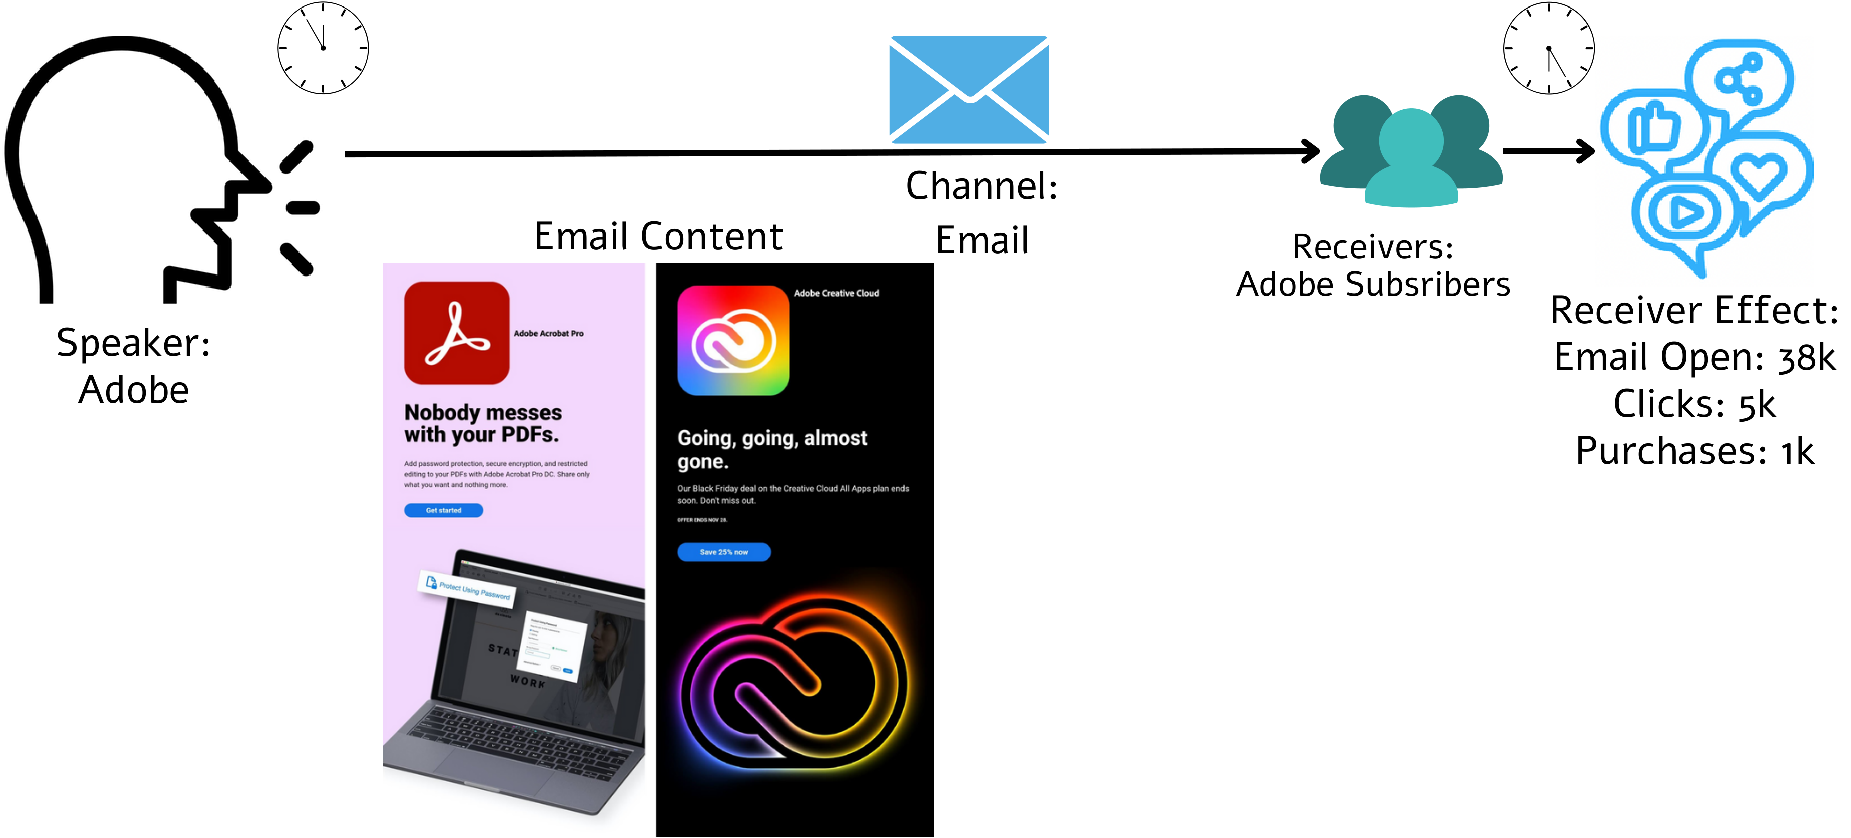
\includegraphics[width=1.0\textwidth]{images/factors of communication.pdf}
  \caption{Communication process can be defined by seven factors: Communicator, Message, Time of message, Channel, Receiver, Time of effect, and Effect. Any message is created to serve an end goal. For marketers, the end goal is to bring in the desired receiver effect (behavior) (like clicks, purchases, likes, and customer retention). The figure presents the key elements in the communication pipeline - the marketer, message, channel, receivers, and finally, the receiver effect.   \label{fig:factors-of-communication}}
\end{figure*}

Historically, social scientists have sought explanations of human behavior that can provide interpretable causal mechanisms behind human functioning. A few prominent examples are Milgram's \cite{milgram1978obedience} and Asch's \cite{asch1948doctrine} experiments on persuasion, explaining the causal mechanism of obedience to authority. The approach of theorizing has worked in physical sciences where the data is plentiful, and theories make unambiguous predictions but have not been too successful in \textit{predicting} social outcomes in behavioral sciences \cite{open2015estimating,tetlock2017expert,forecasting2023insights}. In fact, many studies have shown that expert human opinions fare similar to non-experts (\textit{e.g.}, predicting economic and political trends \cite{tetlock2017expert} and societal change: \cite{forecasting2023insights}), and the opinion of non-expert population is roughly the same as a random coin toss in predicting behavior (\textit{e.g.}, predicting cascades \cite{tan2014effect} or image memorability \cite{isola2013makes}). At the same time, causal mechanisms have their own merits; most notably, they help decision-makers (often humans) to make intuitive sense of the situation and make their next decision based on it. 


In parallel, due to the availability of human behavior data at scale, researchers in machine learning are showing a growing interest in traditionally social scientific topics, such as messaging strategies leading to persuasion \cite{habernal2016makes,kumar2023persuasion,luu2019measuring,bhattacharyya-etal-2023-video}, information diffusion \cite{cheng2014can,martin2016exploring}, and most importantly, prediction and predictability of human behavior \cite{choi2012predicting,song2010limits}. Machine learning approaches bring with them the culture of (training and) testing their models on large real-world datasets and pushing the state-of-the-art in terms of predictive accuracies; at the same time, often, ML approaches can only be operated as black boxes with no direct mechanism to explain predictions \cite{salganik2019bit,singla2022audio}.



In the prediction community, different subfields have emerged dealing with the different parts of the problem of optimization of human behavior. For instance, advertisement personalization studies how to optimize (choose) \textit{receiver} for a given message \cite{chandra2022personalization}, and recommendation systems study how to \textit{choose content} from a set of pre-decided contents for a given receiver to elicit a certain effect \cite{herlocker2004evaluating}. A popular problem within the prediction community is the effect prediction problems, for example, clickthrough (CTR) prediction \cite{mcmahan2013ad}, Twitter cascade prediction \cite{cheng2014can,martin2016exploring}, sales prediction \cite{choi2012predicting,pryzant2017predicting}, content memorability prediction \cite{isola2011makes,khosla2015understanding,si2023long}, \textit{etc}. There are also works to optimize the time of the message to elicit certain effect \cite{newstead2010cost,si2023long}. Therefore, we see that all the factors of communication are studied independently in their own light with the aim of achieving the desired effect. 


%Notably, this is the forward path of communication in which, as time progresses, a message originates, travels in a channel, is received by the subscribers, and finally generates an effect. 
Effect (or behavior) over a content can also enable us to understand about the content, the communicator, the receiver, or the time. Therefore, efforts have also been made to extract information about the content itself from the behavior it generates. For instance, using keystroke movements \cite{plank2016keystroke} and eye movements to improve natural language processing \cite{klerke2016improving,khurana-etal-2023-synthesizing}. Similarly, the fields of human alignment and reinforcement learning with human feedback (RLHF) try to use human behavioral signals of likes, upvotes, downloads, and annotations of a response's helpfulness to improve content generation - both text \cite{kreutzer2018can,stiennon2020learning,ziegler2019fine,nakano2021webgpt,si2023long} and images \cite{lee2023aligning,pressman2023simulacra,wu2023better,khurana2023behavior}.




% XXX: to be improved
In the more traditional social science and computational social science cultures, research is carried out to discover causal effects and model them. 
For instance, propaganda and mass communication studies \cite{mcquail1987mass,krippendorff2018content,lasswell1948structure,lasswell1971propaganda} try to understand the culture, time, authors, recipients in a non-invasive manner using the messages exchanged, and persuasion studies \cite{petty1981effects,chaiken1980heuristic} where the persuasion strategy present in the content is identified and correlated with (un)successful efforts of persuasion. 




A common theme that runs through both research cultures in behavioral sciences is the intent to control behavior. Explanation and prediction are intermediate steps to control and hence optimize behavior. Optimizing behavior means to fulfill the communicator's objectives by controlling the other six parts of the communication process (Fig.~\ref{fig:factors-of-communication}). Due to the problem space being large, the solution needs a general understanding of human behavior as opposed to being domain-specific. 


The characteristic that marks the digital age is the prevalence of human behavioral data in huge repositories. This data is \textit{big} (allowing to model heterogeneity), \textit{always-on} (allowing to look in the past as well as live measurements), observational (as opposed to reactive), but also \textit{incomplete} (does not capture all that is happening everywhere everytime in a single repository) and \textit{algorithmically confounded} (generated as a byproduct of an engineering process with a goal) \cite{salganik2019bit}. While the predictive culture has tried to make use of some of this data in the form of social media datasets like Twitter \cite{tumasjan2010predicting,asur2010predicting} and Instagram \cite{kim2020multimodal}, Google trends \cite{choi2012predicting,carriere2013nowcasting}, Wikipedia \cite{generous2014global,de2021general,mestyan2013early}, shopping websites \cite{krumme2013predictability,de2015unique} and other data sources \cite{brockmann2006scaling,song2010limits,miritello2013limited}, these efforts are limited, in the sense of being dependent on one or a few chosen platforms, able to answer a limited set of questions, and restricted by access to private data. We want a model that can understand (predict and explain) \textit{human behavior in general} as opposed to modeling a particular effect (retweet prediction) on a particular platform (\textit{e.g.} Twitter) for a certain type of users.
This problem carries parallels with the problem being solved in the natural language processing (NLP) community, where supervised models in NLP are limited by the amount of supervision available and being able to answer one question (for which the supervised model was trained). The problem was solved by developing Large Language Models (LLMs), which are general purpose models capable of \textit{understanding language}, and hence can solve natural language tasks like sentiment analysis, question answering, email generation, and language translation in zero-shot (\textit{i.e.} without needing any explicit training for that task) \cite{devlin2018bert,brown2020language,radford2018improving,raffel2020exploring,radford2019language}.





\begin{figure*}[h]
  \centering
  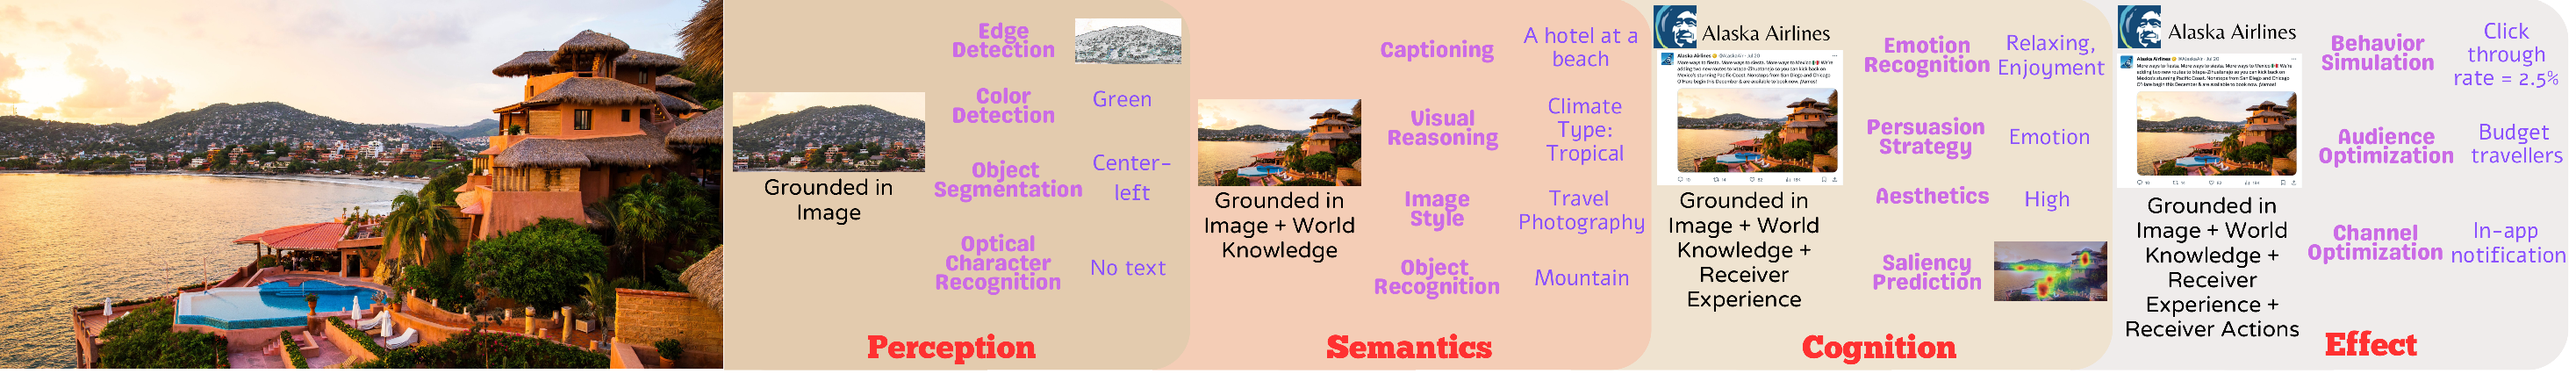
\includegraphics[width=1.0\textwidth]{images/levels of analysis.pdf}
  \caption{Levels of content analysis. The figure lists tasks and their sample outputs arranged in a hierarchy \cite{shannon-weaver-1949}. This is roughly based on levels of language. Notably, humans are good at predicting the first three levels but not the last level \cite{tetlock2017expert,forecasting2023insights,tan2014effect,isola2013makes}. 
  \label{fig:levels of content analysis}
  }
\end{figure*}


Similarly, how do we develop a model capable of understanding behavior \textit{in general}? With the intent to answer this question, we take motivation from LLMs, where the idea is to train a model on a data-rich task. The task chosen to train LLMs is the next-word prediction, and the dataset is the text collected from the entire internet. The next-word prediction task is a data-rich task that can be trained on the huge text repositories from the internet. The intuition is that two approaches have always worked for neural networks: larger model sizes and more data for training \cite{mikolov2013efficient,devlin2018bert,radford2018improving,raffel2020exploring}. Going from a few million tokens of text \cite{mikolov2013efficient,radford2018improving} to a trillion tokens \cite{touvron2023llama,brown2020language} leads to an increase in the transfer learning capability leading to performance improvements over a wide variety of natural language tasks. 


The digital revolution has provided us with huge repositories of data. We leverage the human behavior repositories available on the internet for this general-purpose human behavior model. The format of this data is the general communication model shown in Fig.~\ref{fig:factors-of-communication} consisting of communicator, message, time of message, channel, receiver, time of effect, and effect. Due to the incomplete nature of behavioral repositories, all the factors are usually not always available. However, a subset is always available, and we show that the data scale, along with a large model, helps make a general behavior understanding model \cite{khandelwal2023large}. We call this model, Large Content and Behavior Model (LCBM). We show that LCBM can predict behavior, explain it, and generate a message to bring about certain behavior \cite{khurana2023behavior,si2023long,khandelwal2023large}. 



\textit{Are general LLMs unable to solve behavioral problems?} A question that arises is whether LLMs, which already learn trillions of text tokens, are able to understand and predict behavior. We investigate that question over several large models, including GPT-3.5 \cite{brown2020language}, GPT-4 \cite{openai2023gpt4}, Llama-13 B and LLama-7B \cite{touvron2023llama}, and find that they do not seem to have any behavioral capabilities. The reason for this is that large language models only include one factor (message) out of the 7-factor communication model (Fig.~\ref{fig:factors-of-communication}) while considering other parts as ``noise'' (for instance, see \cite{biderman2022datasheet,penedo2023refinedweb}). This systematic purge of communicator, receiver, channel, time, and, most importantly, behavior causes the models not to develop any behavioral capabilities (Level-C of Shannon and Weaver \cite{shannon-weaver-1949}). As an example, Llava \cite{liu2023visual}, a recent large language and vision model (LVM) trained by connecting a vision encoder with a language model, shows that after training on a few hundred thousand instructions, the language model can now ``see'', and is able to answer questions on the images. However, the questions all lie in the first two levels of content analysis shown in Fig.~\ref{fig:levels of content analysis}. The reason is that the instructions used to align the image encoder with the downstream LLM all lie in the first two levels while ignoring the last two. 
In the upcoming chapters, we explore how we can train a general behavior model and how including back the other factors of communication in training data help in understanding human behavior.


\textit{Outline for the upcoming chapters}: Following the two traditions of social sciences, in this work, in Chapter-\ref{chatper:Explaining Behavior: Persuasion Strategies}, I start with a more traditional approach to behavior explanation, where I cover the first works on extracting persuasion strategies in advertisements (both images and videos) \cite{kumar2023persuasion,bhattacharyya-etal-2023-video}. The contributions of these works include constructing the largest set of generic persuasion strategies based on theoretical and empirical studies in marketing, social psychology, and machine learning literature and releasing the first datasets to enable the study and model development for the same. These works have been deployed to understand the correlation between the kinds of marketing campaigns and customer behavior measured by clicks, views, and other marketing key performance indicators (KPIs). 

Following this, in Chapter-\ref{chatper:Content and Behavior Models}, I delve into the more modern approach of behavior prediction and leveraging the huge repositories of behavior data available. First, we propose models to integrate behavior with relatively smaller language models like BERT \cite{devlin2018bert}, and show that the resultant models can understand content better than the base models \cite{khurana-etal-2023-synthesizing}. Then, we propose an approach to integrate behavior and content together as part of a single model. We call these models Large Content and Behavior Models (LCBM) \cite{khandelwal2023large}. We show that these models can predict and explain behavior. Next, in Chapter-\ref{chatper:Generating Content Leading to Optimal Behavior}, we show that using these models we can generate messages to elicit certain behavior resulting in behavior optimization. We show this both for the domain of text, by taking the illustrative case of memorability and generating content that is more memorable in long-term \cite{si2023long}, and images, by generating images that are more performant, \textit{i.e.}, can result in more likes and downloads \cite{khurana2023behavior}.



\begin{comment}
    They mentioned that the broad problem of communication can be studied at three levels: technical, semantic, and effectiveness. 
    \textbf{Level A: Technical.} How accurately can the symbols of communication be transmitted?
    
    \textbf{Level B: Semantic.} How precisely do the transmitted symbols convey the desired meaning?
    
    \textbf{Level C: Effectiveness.} How well does the received meaning induce the desired conduct in the receiver?
    
    These three levels build on top of each other. Thus, solving the problem at Level C necessarily requires solving the corresponding problems at Levels A and B.
    
    Since the publication of this seminal paper, the tremendous growth in the field of telecommunications, particularly the advent of the Internet and mobile devices, has led to affordable, wide-scale solutions for Level A.
    With the recent advances in large language models (LLMs) such as BERT \citep{devlin2018bert}, GPT-3 and 4 \citep{brown2020language,openai2023gpt4}, T5 \citep{raffel2020exploring}, and many more, we have witnessed a significant improvement in the performance of various Natural Language Processing (NLP) tasks. LLMs in zero- or few-shot settings can easily handle tasks such as question answering, summarization, translation, and many more. This has helped us progress towards solving Level B to a large extent. However, there has been limited progress in Level C, the effectiveness problem. 
    
    
    
    Effectiveness refers to communicating to fulfill the communicator's objectives.
\end{comment}


%%%%%%%%%%%%%%%%%%%%%%%%%%%%%%%%%%%%%%%%
%%%%%%%%%%%%%%%%%%%%%%%%%%%%%%%%%%%%%%%%
%%%%%%%%%%%%%%%%%%%%%%%%%%%%%%%%%%%%%%%%
%%%%%%%%%%%%%%%%%%%%%%%%%%%%%%%%%%%%%%%%

\chapter{Explaining Behavior: Persuasion Strategies}
\label{chatper:Explaining Behavior: Persuasion Strategies}


\begin{figure}[t]
    % \vspace{-38mm}
    \centering
    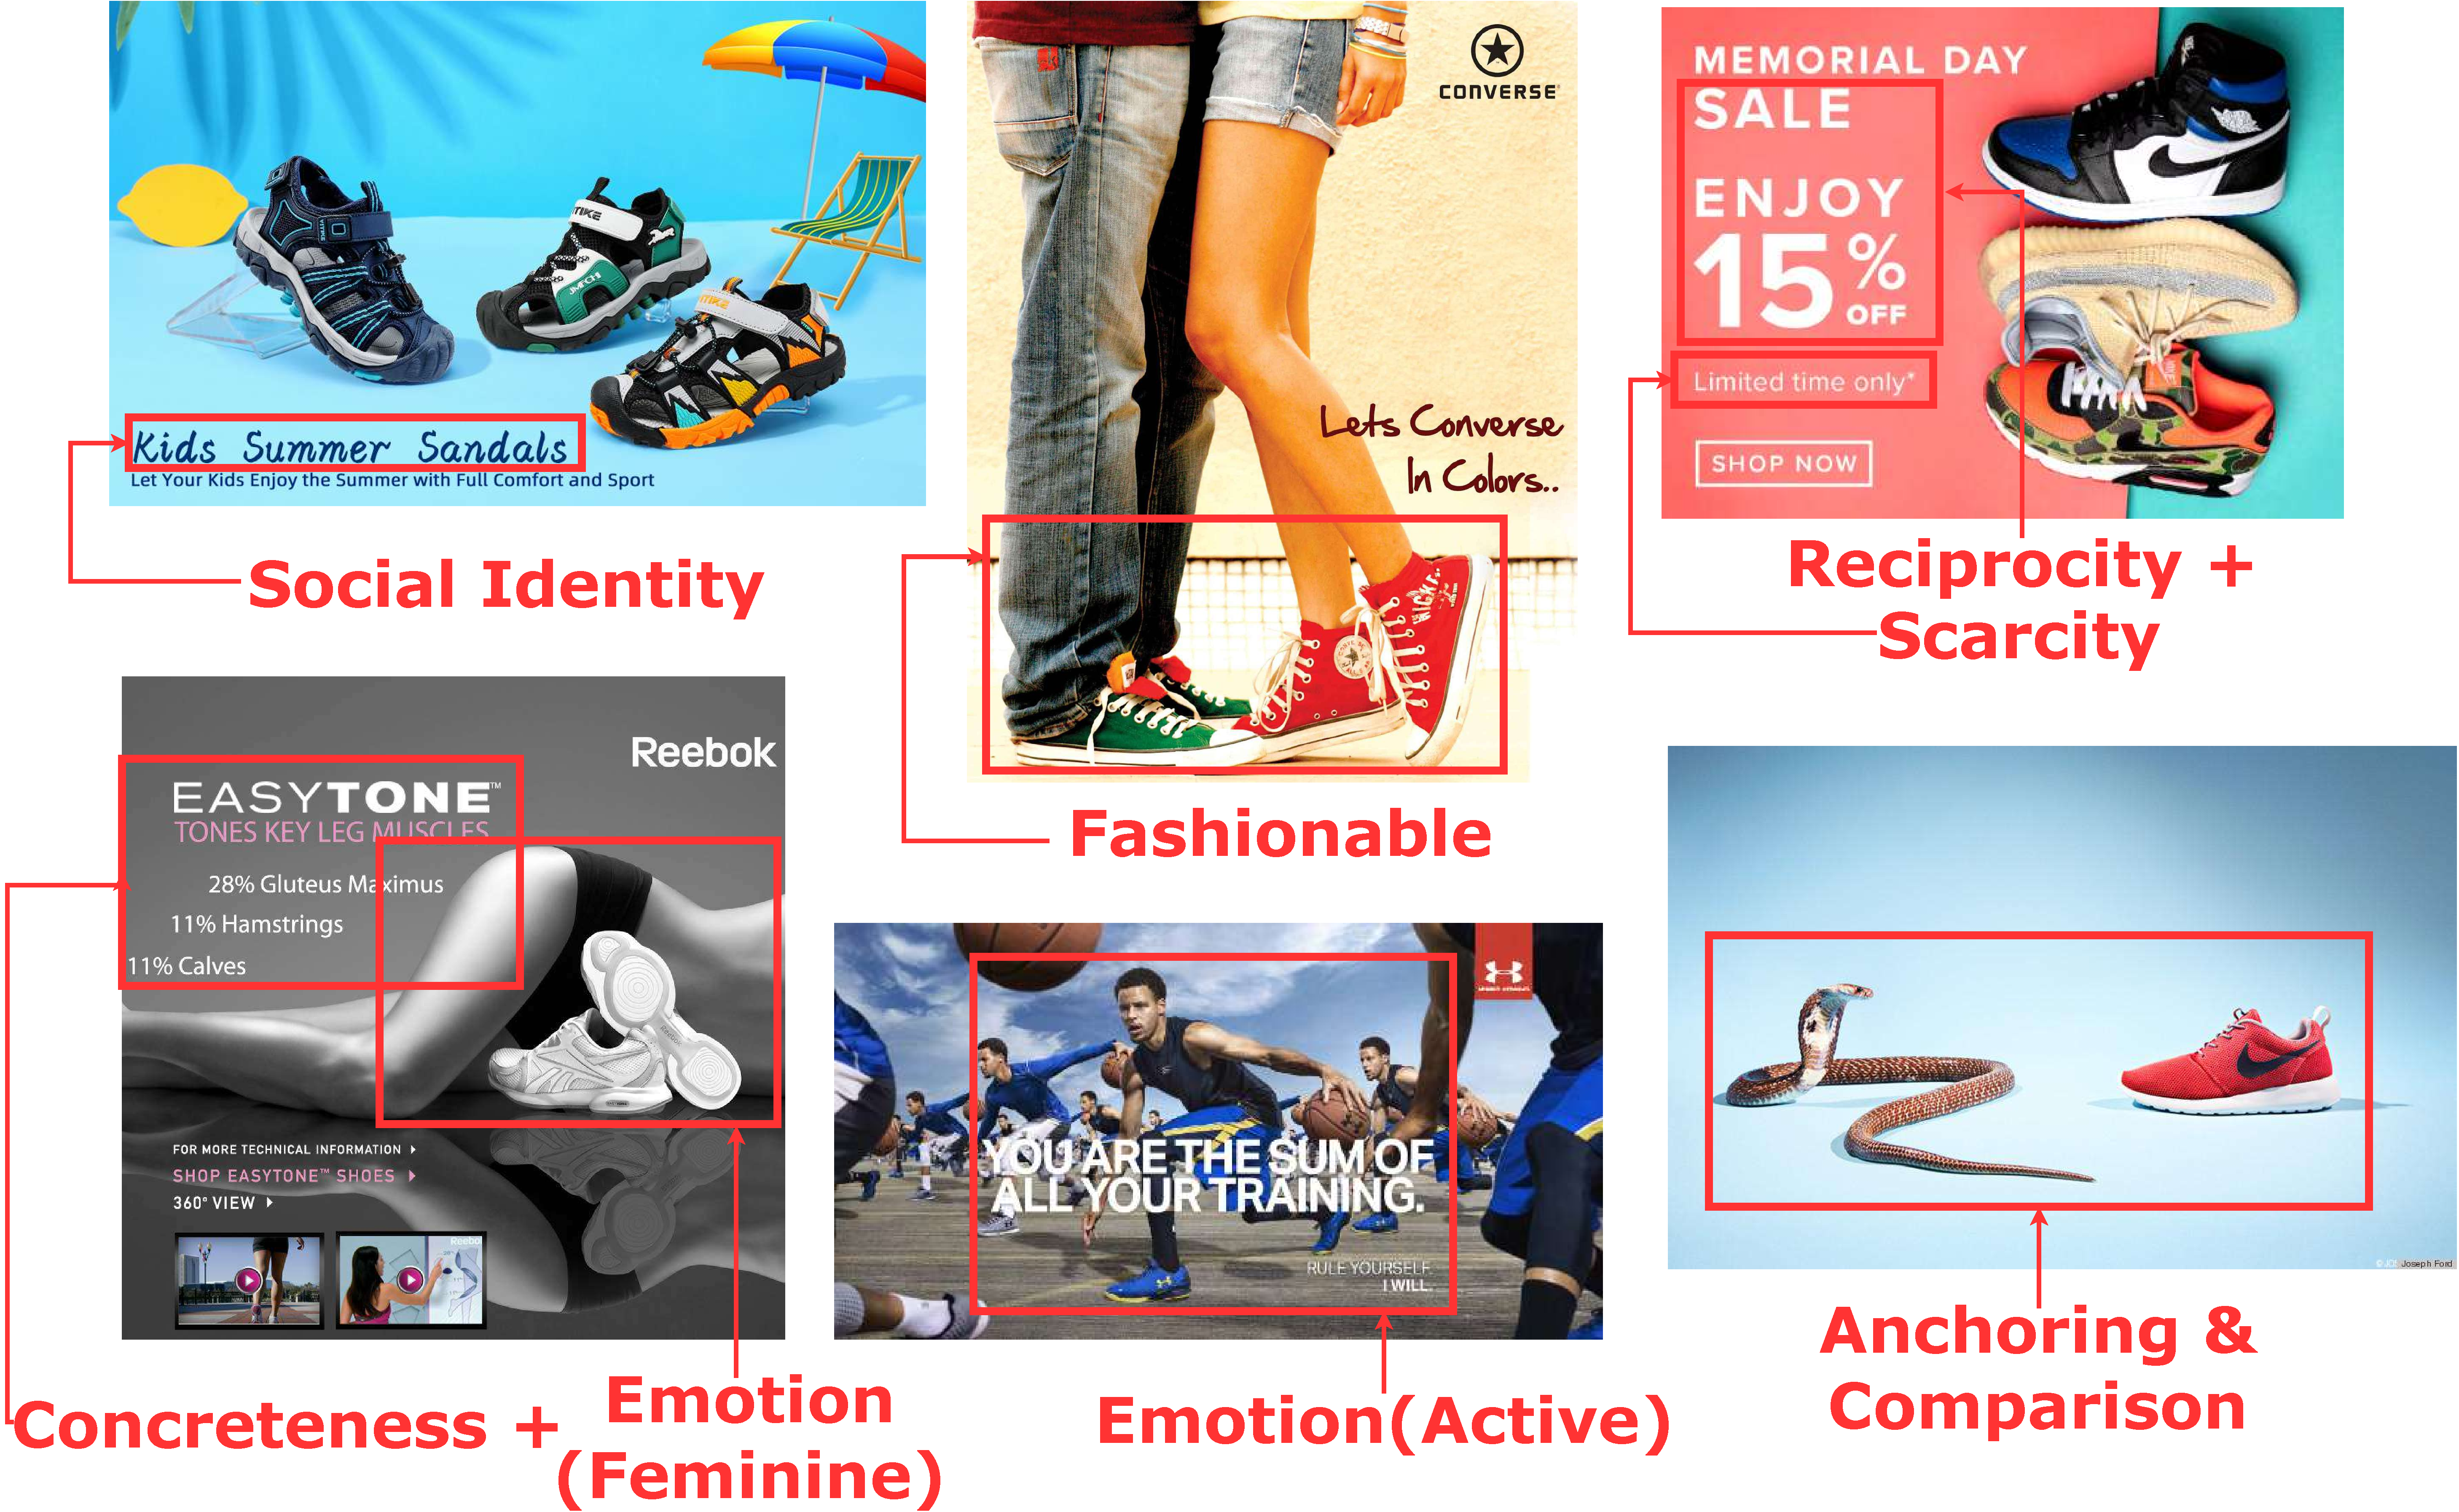
\includegraphics[scale=0.08]{images/footwear-strategies.pdf}
    \caption{Different persuasion strategies are used for marketing the same product (footwear in this example). The strategies are in red words and to be defined by us in the paper.}
    \label{fig:footwear-strategies}
    % \vspace*{-4mm}
\end{figure}


\begin{figure*}[!ht]
    \centering
    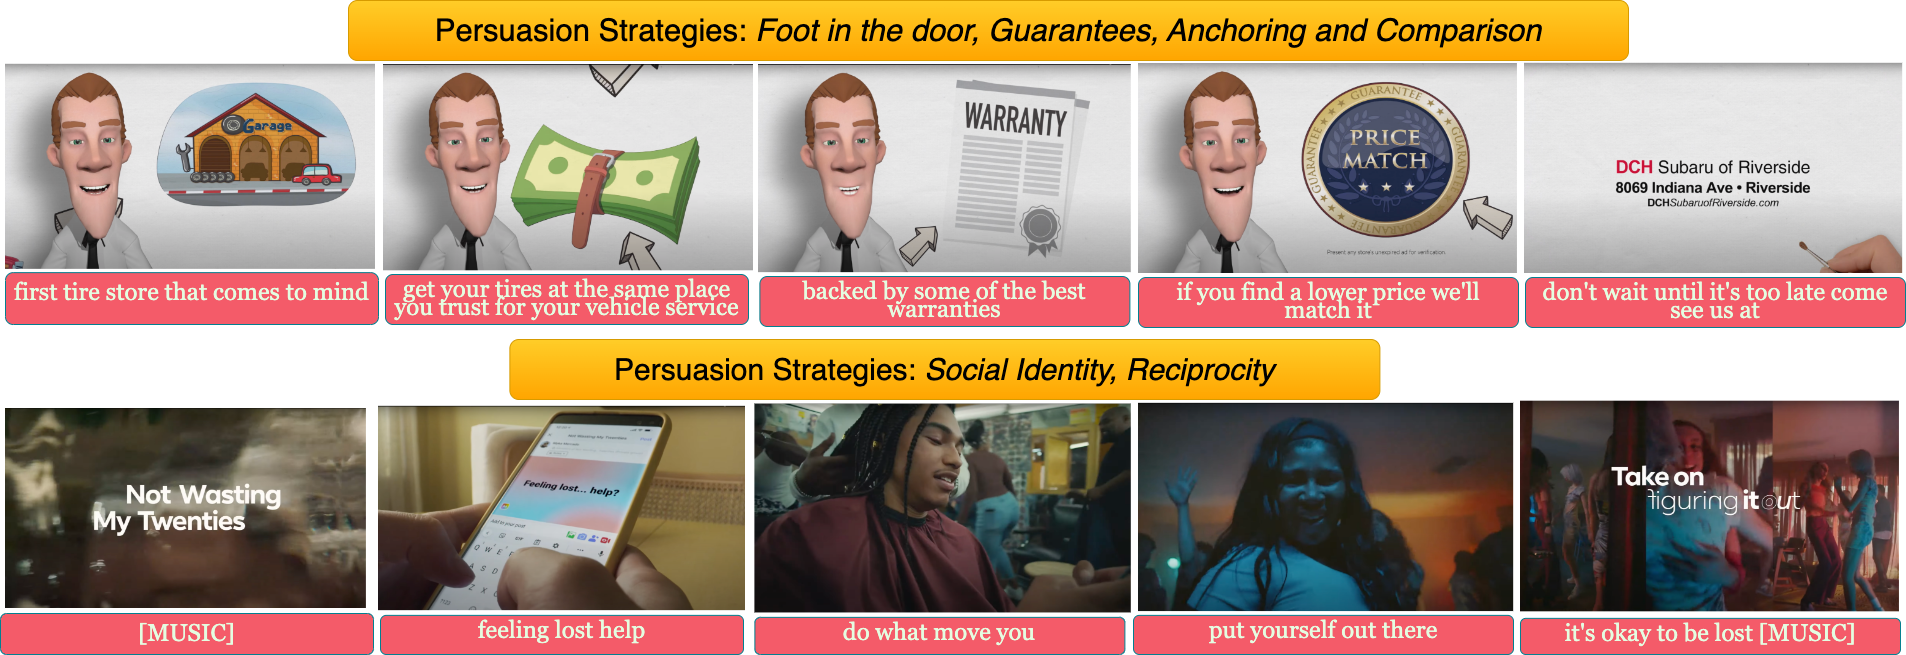
\includegraphics[width=\textwidth]{images/persuasion-strategies-videos.png}
    \caption{Examples of videos with their annotated persuasion strategies. Relevant keyframes and ASR captions are shown in the figure, along with the annotated strategies. These two videos can be watched at 
    \url{https://bit.ly/3Ie3JG0}, \url{https://bit.ly/3OgtLwj}
    .}
    \label{fig:persuasion-strategy-dataset-examples}
\end{figure*}



 Modeling what makes an advertisement persuasive, \textit{i.e.}, eliciting the desired response from consumer, is critical to the study of propaganda, social psychology, and marketing. Despite its importance, computational modeling of persuasion in computer vision is still in its infancy, primarily due to the lack of benchmark datasets that can provide persuasion-strategy labels associated with ads. Motivated by persuasion literature in social psychology and marketing, we introduce an extensive vocabulary of persuasion strategies and build the first ad corpus (both image and video) annotated with persuasion strategies. We then formulate the task of persuasion strategy prediction with multi-modal learning. The image dataset also provides image segmentation masks, which labels persuasion strategies in the corresponding ad images on the test split. We publicly release our code and dataset at \url{https://midas-research.github.io/persuasion-advertisements/}. This chapter is based on two papers I published along with collaborators \cite{kumar2023persuasion,bhattacharyya-etal-2023-video}.




Marketing communications is the mode by which companies and governments inform, remind, and persuade their consumers about the products they sell. They are the primary means of connecting brands with consumers through which the consumer can know what the product is about, what it stands for, who makes it, and can be motivated to try it out. To introduce meaning into their communication, marketers use various rhetorical devices in the form of persuasion strategies such as \textbf{emotions} ({\it e.g.}, Oreo's ``Celebrate the Kid Inside'', humor by showing Ronald McDonald sneaking into the competitor Burger King's store to buy a burger), \textbf{reasoning} ({\it e.g.}, ``One glass of Florida orange juice contains 75\% of your daily vitamin C needs''), \textbf{social identity} ({\it e.g.}, Old Spice's ``Smell like a Man''), and \textbf{impact} ({\it e.g.}, Airbnb showing a mother with her child with the headline ``My home is funding her future'') (Refer to Fig.~\ref{fig:rhetoric-strategies-ads} to see these ads). Similarly, even for marketing the same product, marketers use different persuasion strategies to target different demographies (see Fig.~\ref{fig:footwear-strategies}). Therefore, recognizing and understanding persuasion strategies in ad campaigns is vitally important to decipher viral marketing campaigns, propaganda, and enable ad-recommendation. 




\begin{figure*}
    \centering
    \begin{subfigure}[b]{0.22\textwidth}
         \centering
         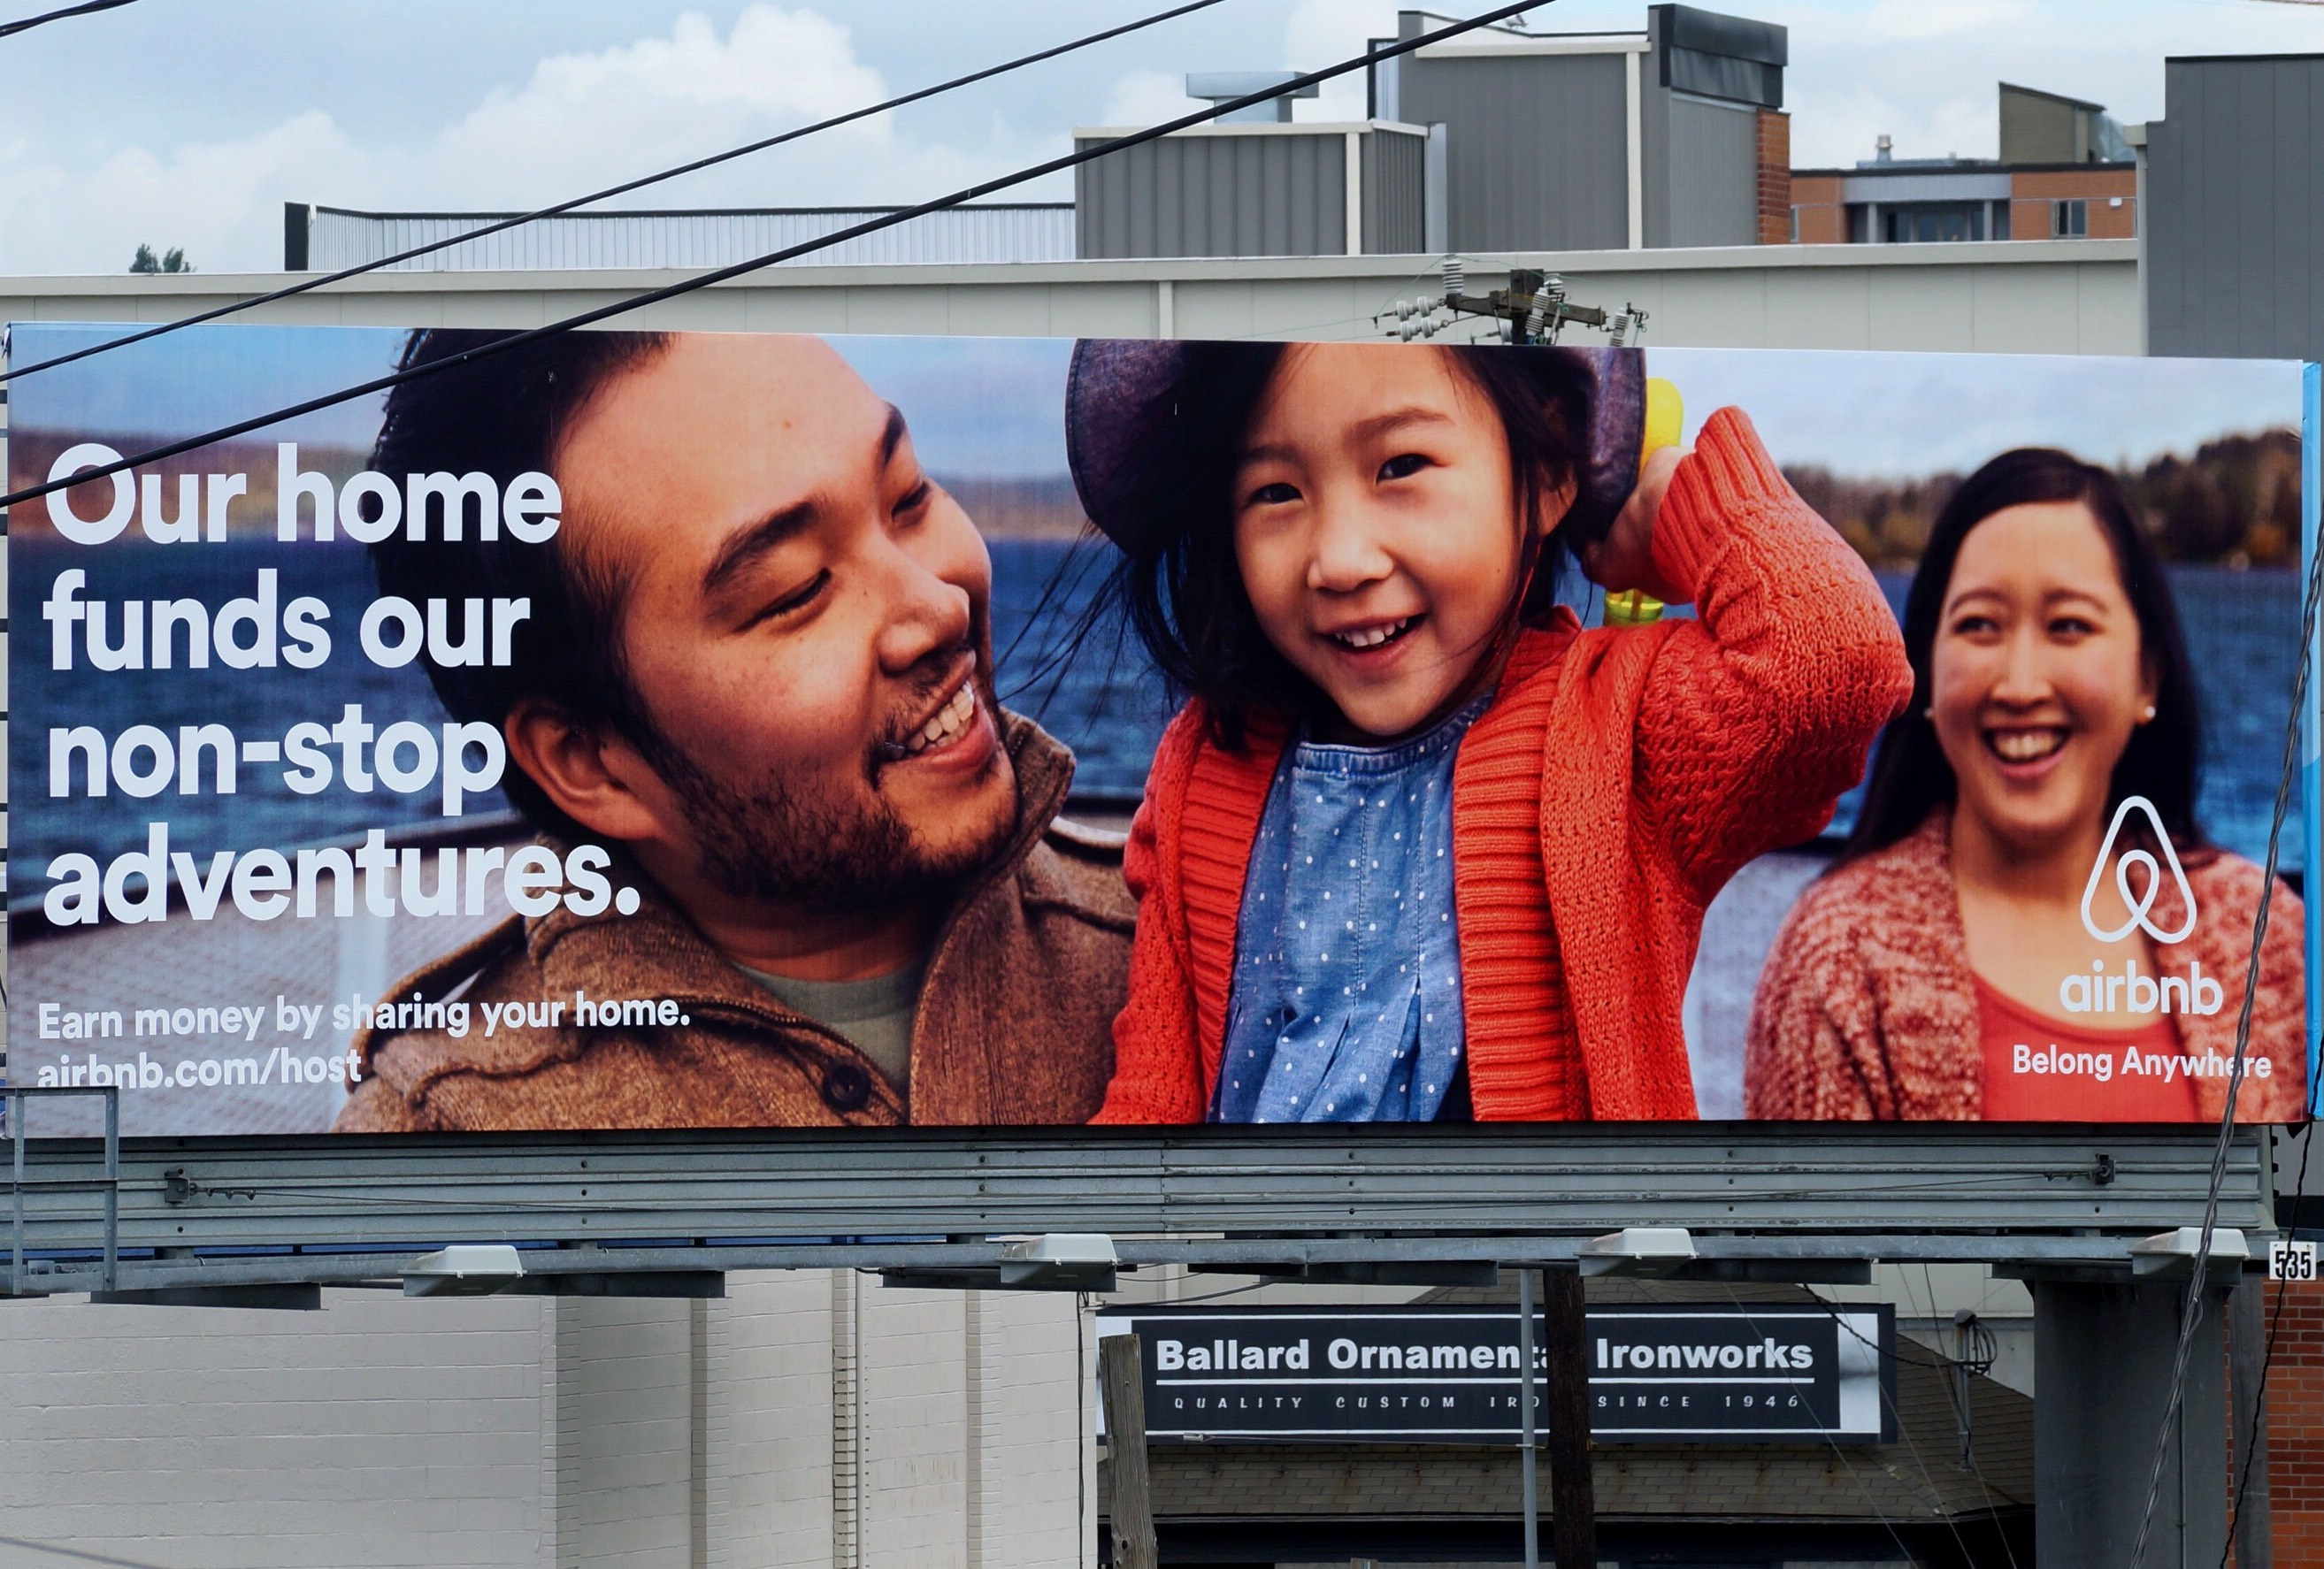
\includegraphics[width=\textwidth,scale=0.6]{images/airbnb.jpeg}
         \caption{}
         \label{fig:Airbib}
     \end{subfigure}
     \begin{subfigure}[b]{0.2\textwidth}
         \centering
         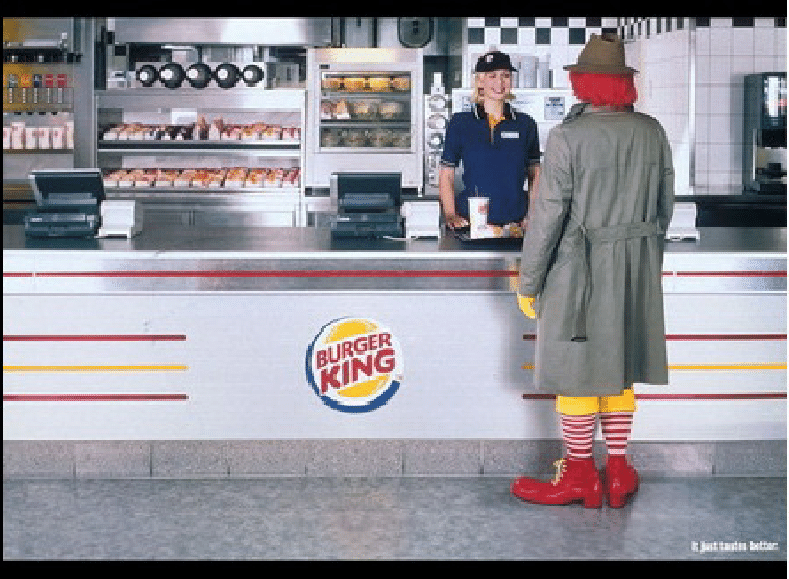
\includegraphics[width=\textwidth,scale=0.5]{images/Burger-King-vs-McDonalds-comparative-ad.png}
         \caption{}
         \label{fig:mcdonald}
     \end{subfigure}
     \begin{subfigure}[b]{0.27\textwidth}
         \centering
         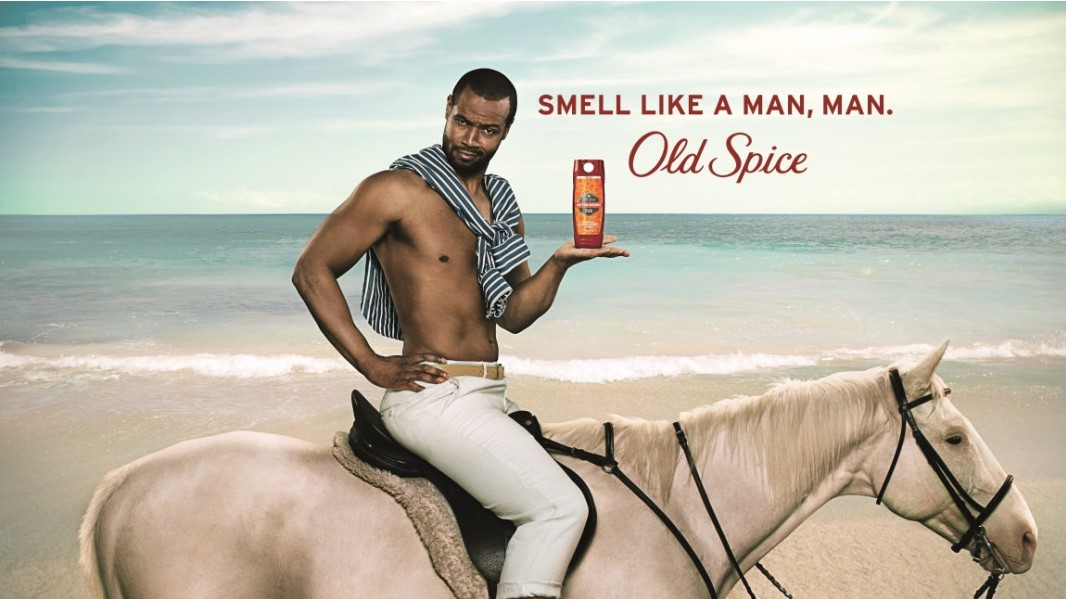
\includegraphics[width=\textwidth,scale=1.0]{images/old-spice.jpeg}
         \caption{}
         \label{fig:old-spice}
     \end{subfigure}
     \begin{subfigure}[b]{0.12\textwidth}
         \centering
         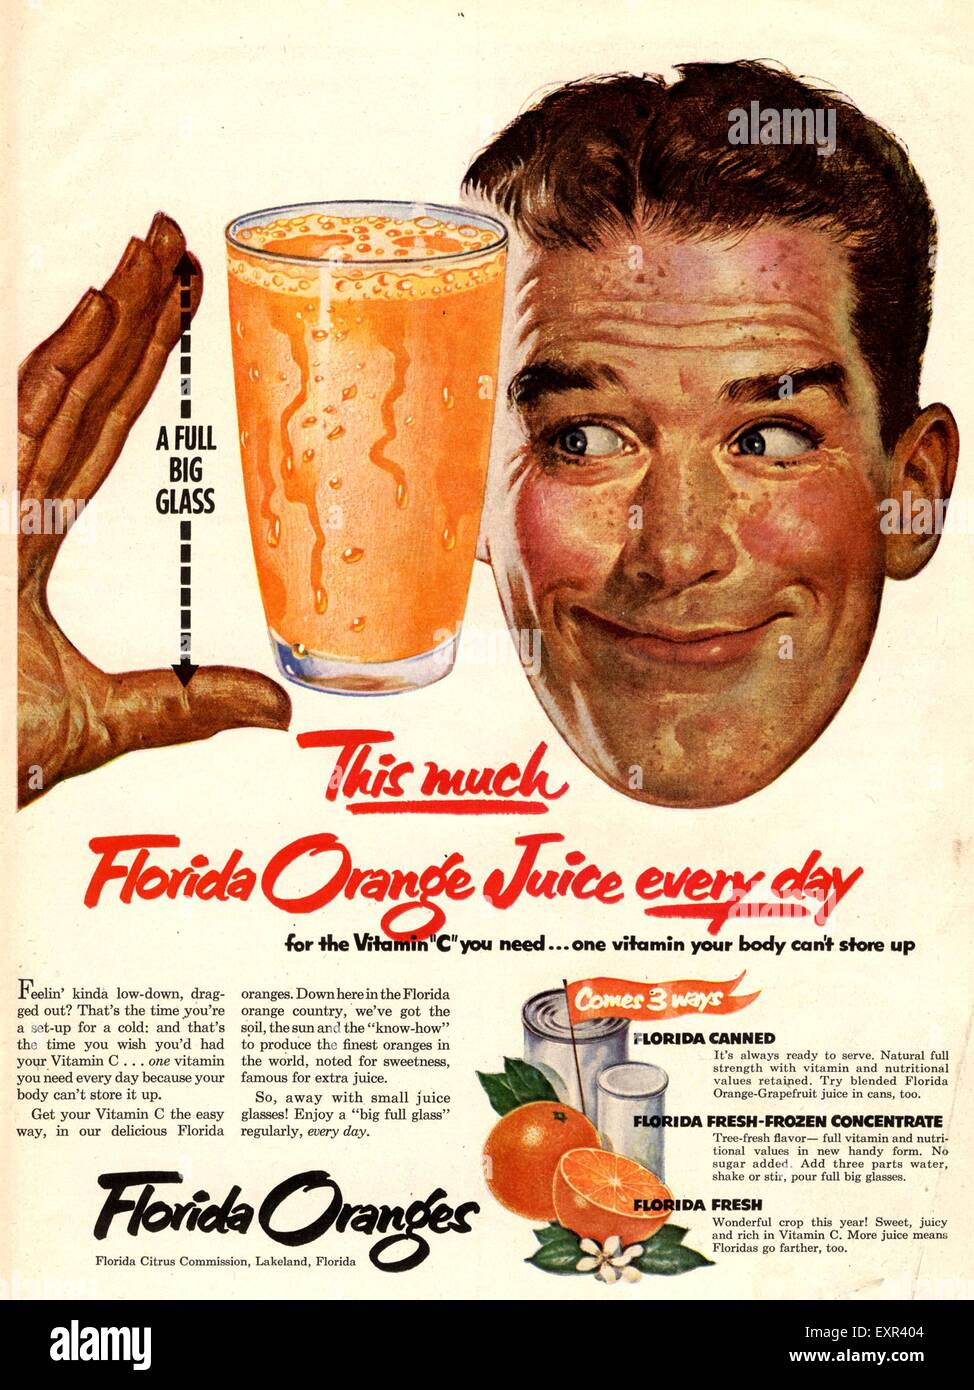
\includegraphics[width=\textwidth,scale=0.68]{images/1950s-usa-florida-orange-juice-magazine-advert-EXR404.jpeg}
         \caption{}
         \label{fig:florida-juice}
     \end{subfigure}
     \begin{subfigure}[b]{0.12\textwidth}
         \centering
         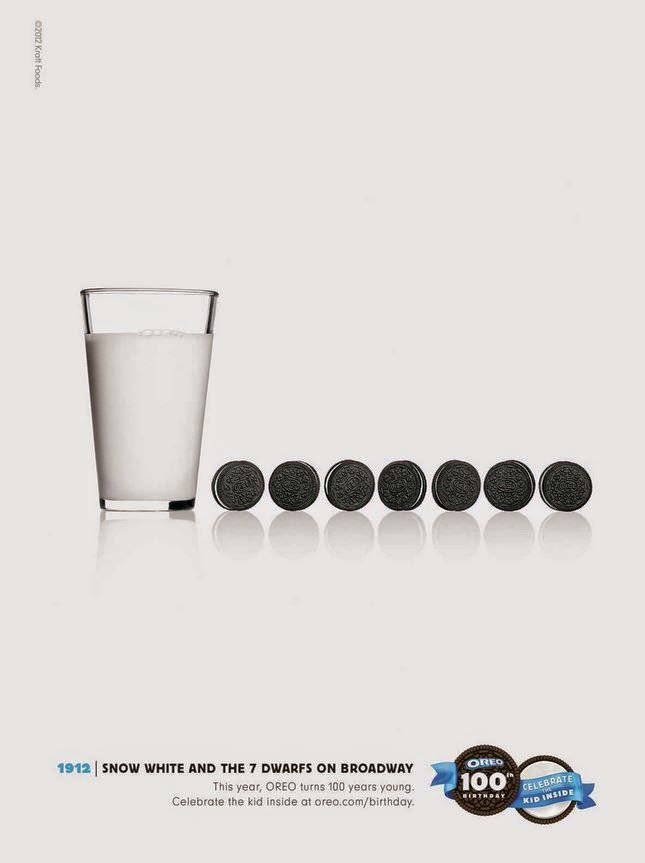
\includegraphics[width=\textwidth,scale=0.68]{images/Oreo_SnowWhite.jpeg}
         \caption{}
         \label{fig:oreo}
     \end{subfigure}
     
     
    \caption{Various rhetoric strategies used in advertisements}
    \label{fig:rhetoric-strategies-ads}
\end{figure*}




Studying rhetorics of this form of communication is an essential part of understanding visual communication in marketing. Aristotle, in his seminal work on rhetoric, underlining the importance of persuasion, equated studying rhetorics with the study of persuasion\footnote{``Rhetoric may be defined as the faculty of discovering in any particular case all of the available means of \textit{persuasion}'' \cite{rapp2002aristotle}} \cite{rapp2002aristotle}. While persuasion is studied extensively in social science fields, including marketing \cite{meyers1999consumers,keller2003affect} and psychology \cite{hovland1953communication,petty1986elaboration}, computational modeling of persuasion in computer vision is still in its infancy, primarily due to the lack of benchmark datasets that can provide representative corpus to facilitate this line of research. In the limited work that has happened on persuasion in computer vision, researchers have tried to address the question of which image is more persuasive \cite{bai2021m2p2} or extracted low-level features (such as emotion, gestures, and facial displays), which indirectly help in identifying persuasion strategies without explicitly extracting the strategies themselves \cite{joo2014visual}. On the other hand, decoding persuasion in textual content has been extensively studied in natural language processing from both extractive, and generative contexts \cite{habernal2016makes,ChenYang2021,luu2019measuring}. This forms the motivation of our work, where we aim to identify the persuasion strategies used in visual content such as advertisements.




%In the limited work which has happened in computer vision domain for studying advertisements, researchers have investigated topics, sentiments, action-reason (containing \textit{what} the viewer should do and \textit{why} they should do it, according to the ad) statements \cite{hussain2017automatic,ye2018advise,ye2019interpreting}, or other features such as emotion, gestures, and facial display types in ads \cite{huang2016inferring,joo2014visual,DBLPconfbmvc0004K18}. While the prior computer vision work was important for finding the lower-level content properties of advertisements, studying advertisement rhetoric involves integrating the above lower-level elements to form \textit{persuasive message appeals}. %atkinson2019gets,carlile2018give,stab2014annotating,althoff2014ask,iyer2019unsupervised,rosenthal2017detecting,yang2019let,stab2017parsing,tan2016winning,wang-etal-2019-persuasion,zhang2016inferring,duerr2021persuasive,anand2011believe,chen2021weakly,hidey2017analyzing,he2018decoupling,durmus-cardie-2018-exploring,wachsmuth2017computational,longpre2019persuasion,shaikh-etal-2020-examining} use cases, and in  %




The systematic study of persuasion began in the 1920s with the media-effects research by Lasswell \cite{lasswell1971propaganda}, which was used as the basis for developing popular models of persuasion, like the Elaboration Likelihood Model (ELM) \cite{petty1986elaboration}, Heuristic Systematic Model (HSM) \cite{chaiken1980heuristic}, and Hovland's attitude change approach \cite{hovland1953communication}. %Amongst these, the most widely accepted model of persuasion theory is the Elaboration Likelihood Model (ELM). 
Laswell in this research broke down communication into five factors by defining communication as an act of \textit{who} said it, \textit{what} was said, in \textit{what} channel it was said, to \textit{whom} it was said, and with what \textit{effect} it was said. Later, this model was used as the basis for developing popular models of persuasion, like Elaboration Likelihood Model \cite{petty1986elaboration}, Heuristic Systematic Model \cite{chaiken1980heuristic}, and Hovland's attitude change approach \cite{hovland1953communication}. Amongst these, the most widely accepted model of persuasion theory is the Elaboration Likelihood Model (ELM). 

These models of persuasion posit a dual process theory that explains attitude and behavior change (persuasion) in terms of the following major factors: stimuli (messages), personal motivation (the desire to process the message), capability of critical evaluation, and cognitive busyness. These factors could be divided into cognitive, behavioral, and affective processes of attitude change. 
Thus, a person may begin liking a new political candidate because she just donated \$100 to the campaign (behavior-initiated change), because the theme music in a recently heard commercial induced a general pleasantness (affect-initiated change), or because the person was impressed with the candidate’s issue positions (cognitive initiated change). Similarly, if a person already likes a political candidate he may agree to donate money to the campaign (behavioral influence), may feel happiness upon meeting the candidate (affective influence), and may selectively encode the candidate’s issue positions (cognitive influence) \cite{petty1986elaboration}.

ELM posits that when facing a message from a persuader, the persuadee reacts by using the two information processing channels: central processing or peripheral processing. When the persuadee processes information centrally, the cognitive responses, or elaborations, will be much more relevant to the information, whereas when processing peripherally, the individual may rely on heuristics and other rules of thumb when elaborating on a message. The factors which influence how and how much one will elaborate the persuasive message is given by the message type, personal motivation, and other factors presented in the ELM. Being at the high end of the elaboration continuum, people assess object-relevant information in relation to schemas that they already possess, and arrive at a reasoned attitude that is supported by information \cite{van2011handbook}. 

In this chapter, we build on these psychological insights from persuasion models in sociology and marketing and study the message strategies that lead to persuasion. We codify, extend, and unify persuasion strategies studied in the psychology and marketing literature into a set of 20 strategies divided into 9 groups (see Fig.~\ref{fig:persuasion-strategies-headline-image}, Table~\ref{tab:persuasive-strategies-list}): \textit{Authority and Credibility}, \textit{Social Identity and Proof}, where cognitive indirection in the form of group decisioning and expert authority is used for decisions, \textit{Value and Impact Formulation} where logic is used to explain details and comparisons are made, \textit{Reciprocity}, \textit{Foot in the door}, \textit{Overcoming Resistance} where social and cognitive consistency norms are harnessed to aid decision-making, \textit{Scarcity}, \textit{Anthropomorphism} and \textit{Emotion} where information is evaluated from the lenses of feelings and emotions. In addition to introducing the most extensive vocabulary for persuasion strategies, we make a superset of persuasion strategies presented in the prior NLP works, which introduced text and domain-specific
persuasion tactics, thus making large-scale understanding of persuasion across multiple contexts comparable and replicable.


Constructing a large-scale dataset containing persuasion strategies labels is time-consuming and expensive. We leverage active learning to mitigate the cost of labeling fine-grained persuasion strategies in advertisements. We first introduce an attention-fusion model trained in a multi-task fashion over modalities such as text, image, and symbolism. We use the action-reason task from the Pitts Ads dataset \cite{hussain2017automatic} to train the model and then annotate the raw ad images from the same dataset for persuasion strategies based on an entropy based active learning technique.


%As an interesting use case, we extract 1600 raw ad images of Fortune-500 companies using the Facebook Ads API\footnote{\url{https://www.facebook.com/ads/library/api/}}. Then, using the model trained for persuasion strategies, we labelled and analyzed the advertisement campaigns on different companies and industry segments. We find that (\S\ref{sec:Case Study}).


To sum up, our contributions include:\\
1. We construct the largest set of generic persuasion strategies based on theoretical and empirical studies in marketing, social psychology, and machine learning literature. \\
2. We introduce the first dataset for studying persuasion strategies in advertisements. This enables initial progress on the challenging task of automatically understanding the messaging strategies conveyed through visual advertisements. We also construct a prototypical dataset containing image segmentation masks annotating persuasion strategies in different segments of an image.\\
3. We formulate the task of predicting persuasion strategies with a multi-task attention fusion model.\\
4. We conduct extensive experiments on the released corpus,
showing the effect of different modalities on identifying persuasion
strategies, correlation between strategies and topics
and objects with different strategies.\\

\begin{figure*}[t]
% \vspace*{-12mm}
        \centering
        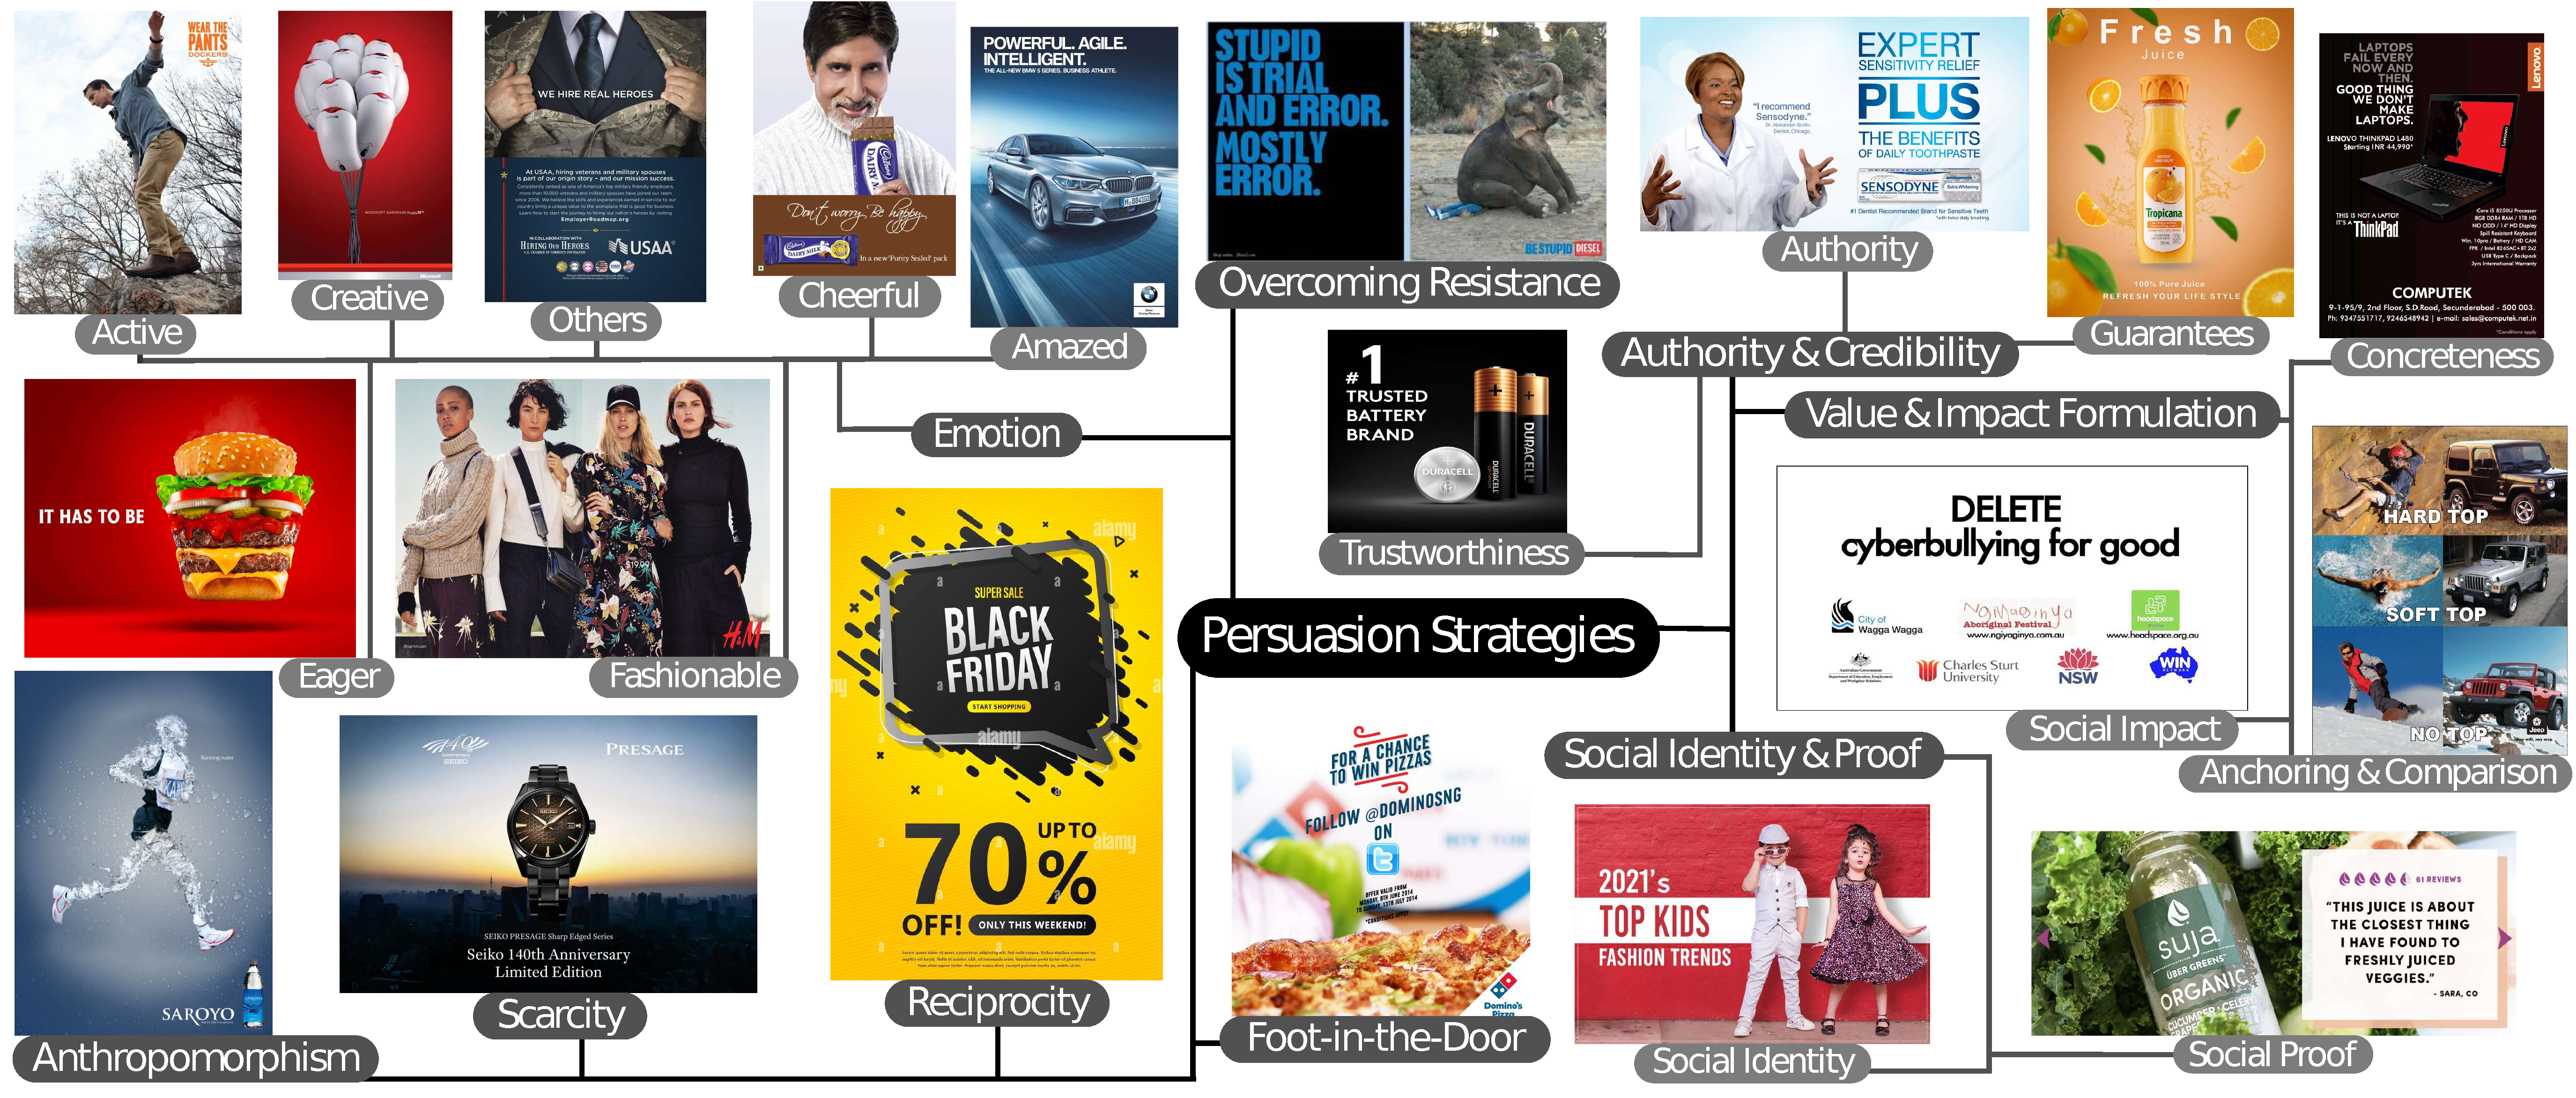
\includegraphics[width=\textwidth]{images/flowchart.pdf}
        \caption{\small \looseness=-1 Persuasion strategies in advertisements. Marketers use both text and vision modalities to create ads containing different messaging strategies. Different persuasion strategies are constituted by using various rhetorical devices such as slogans, symbolism, colors, emotions, allusion.}
        \label{fig:persuasion-strategies-headline-image}
% \vspace*{-4mm}
\end{figure*}

\section{Related Work}
\label{sec:related work}


\textit{How do messages change people's beliefs and actions?} The systematic study of persuasion has captured researchers’ interest since the advent of mass influence mechanisms such as radio, television, and advertising. Work in persuasion spans across multiple fields, including psychology, marketing, and machine learning. 


\textbf{Persuasion in Marketing and Social Psychology:} Sociology and communication science has studied persuasion for centuries now starting from the seminal work of Aristotle on rhetoric. Researchers have tried to construct and validate models of persuasion. Due to space constraints, while we cannot cover a complete list of literature, in Section~\ref{tab:persuasive-strategies-list}, we list the primary studies which originally identified the presence and effect of various persuasion tactics on persuadees. We build on almost a century of this research and crystallize them into the persuasion strategies we use for annotation and modeling. %Using both expenditure and income calculations, \citet{mccloskey1995one} calculate that roughly one quarter of the US GDP in 1994 was due to persuasion. 
Any instance of (successful) persuasion is composed of two events: (a) an attempt by the persuader, which we term as the persuasion strategies, and (b) subsequent uptake and response by the persuadee \cite{anand2011believe,vakratsas1999advertising}. In this work, we study (a) only while leaving (b) for future work. Throughout the rest of the paper, when we say persuasion strategy, we mean the former without considering whether the persuasion was successful or not. 



\textbf{Persuasion in Machine Learning:} Despite extensive work in social psychology and marketing on persuasion, most of the work is qualitative, where researchers have looked at a small set of messages with various persuasion strategies to determine their effect on participants. Computational modeling of persuasion is still largely lacking. In the limited work in computational modeling of persuasion, almost all of it is concentrated in the NLP literature, with only very few works in computer vision.
Research on persuasion in NLP under the umbrella of argumentation mining is broadly carried out from three perspectives: extracting persuasion tactics, studying the effect of constituent factors on persuasion, and measurement of persuasiveness nature of content. A few examples of research studies that annotate persuasive strategies in various forms of persuader-persuadee interactions like discussion forums, social media, blogs, academic essays, and debates are \cite{anand2011believe,tan2016winning,chen2021weakly}. We use these and other studies listed in Section~\ref{tab:persuasive-strategies-list} to construct our vocabulary of persuasion strategies in advertisements. 

Other studies focus on factors such as argument ordering \cite{shaikh-etal-2020-examining,li-etal-2020-exploring-role}, target audience \cite{lukin-etal-2017-argument}, and prior beliefs \cite{el-baff-etal-2020-analyzing} for their effect in bringing about persuasion. Studies such as \cite{althoff2014ask,wei2016post} also try to measure persuasiveness and generate persuasive content. The generation of persuasive (textual) messages has been studied \cite{donadello2020explaining} and, in particular, a novel ML method for learning user model tailored persuasion strategy has also been proposed \cite{hadoux2021strategic, donadello2022machine}.



As one of the first works in the limited work in the computer vision domain, Joo \textit{et al.} \cite{joo2014visual} introduced syntactical and intent features such as facial displays, gestures, emotion, and personality, which result in persuasive images. Their analysis was done on human images, particularly politicians, during their campaigns. %\citet{huang2016inferring} built on top of their dataset to improve their results by using finetuned CNNs. 
Their work on political campaigners is more restrictive than general product and public-service advertisements. Moreover, they deal with low-level features such as gestures and personality traits depicted through the face, which are important for detecting persuasion strategies but are not persuasion strategies themselves. Recently, Bai \textit{et al.} \cite{bai2021m2p2} studied persuasion in debate videos where they proposed two tasks: debate outcome prediction and intensity of persuasion prediction. Through these tasks, they predict the persuasiveness of a debate speech, which is orthogonal to the task of predicting the strategy used by the debater. Other similar works which discuss persuasiveness of images and videos are \cite{joo2015automated,siddiquie2015exploiting}.


%\noindent \textbf{Active Learning} tackles the problem of selecting samples from unlabeled sets to be annotated by an oracle. In the last decade, several active learning strategies have been proposed and applied to several research fields, including speech recognition \cite{hakkani2002active}, natural language processing \cite{thompson1999active}, chemistry \cite{duros2017human}. We refer the reader to the survey of \citet{settles2009active} for an extensive review of active learning methods. Many studies including \citet{collins2008towards,miller_linder_mebane_2020,mullapudi2021learning} have practically applied active learning to annotate datasets and shown substantial improvement in labelling budget and time. 




\section{Generic Taxonomy of Persuasion Strategies}
\label{tab:persuasive-strategies-list}
This section introduces the generic taxonomy of persuasive strategies, their definitions, examples, and connections with prior work. Representative literature from a)~\texttt{SPM}: Social Psychology and Marketing, b)~\texttt{ML}: Machine Learning

\begin{enumerate}
    \item Authority and Credibility: \texttt{SPM}:\cite{aronson1963communicator,milgram1978obedience,cialdini2007influence,milgram1963behavioral,mcginnies1980better,giffin1967contribution,petty1986elaboration} \texttt{ML}:\cite{anand2011believe,iyer2019unsupervised,wachsmuth2017computational,ChenYang2021,durmus-cardie-2018-exploring}
    \begin{enumerate}
        \item \textbf{Guarantees}: Guarantees reduce risk and people try out such products more often. 

        \item \textbf{Authority}: Authority indicated through expertise, source of power, third-party approval, credentials, and awards
    
        \item \textbf{Trustworthiness}: Trustworthiness indicated honesty and integrity of the source through tropes like years of experience, ``trusted brand'', numbers and statistics
    \end{enumerate}

    \item Social Identity and Proof: \texttt{SPM}:\cite{deutsch1955study,petty1997attitudes,wood2000attitude,cialdini2004social,levesque2020human} \texttt{ML}: \cite{anand2011believe,iyer2019unsupervised,rosenthal2017detecting,yang2019let,zhang2016inferring,stab2017parsing,althoff2014ask,hidey2017analyzing,durmus-cardie-2018-exploring}

    \begin{enumerate}
        \item \textbf{Social Identity}: \textit{Normative} influence, which involves conformity with the positive expectations of ``another'', who could be ``another person, a group, or one's self'' (includes self-persuasion, fleeting attraction, alter-casting, and exclusivity)

        \item \textbf{Social Proof}: \textit{Informational influence} by accepting information obtained from others as evidence about reality, \textit{e.g.}, customer reviews and ratings 
    \end{enumerate}

    \item  Reciprocity: \texttt{SPM}:\cite{regan1971effects,cialdini2007influence,clark1984record,clark1979interpersonal,clark1986keeping} \texttt{ML}:\cite{anand2011believe,iyer2019unsupervised,althoff2014ask,ChenYang2021,shaikh-etal-2020-examining}
    \begin{enumerate}
        \item \textbf{Reciprocity}: By \textit{obligating} the recipient of an act to repayment in the future, the rule for reciprocation begets a sense of future obligation, often unequal in nature
    \end{enumerate}

    \item Foot in the door: \texttt{SPM}: \cite{freedman1966compliance,burger1999foot,cialdini2007influence} \texttt{ML}:\cite{chen2021weakly,wang-etal-2019-persuasion,vargheese2020exploring}
    \begin{enumerate}
        \item \textbf{Foot in the door}: Starting with small requests followed by larger requests to facilitate compliance while maintaining \textit{cognitive coherence}.
    \end{enumerate}

    \item  Overcoming Resistance: \texttt{SPM}:\cite{mcguire1961relative,knowles2004resistance,mcguire1964inducing} \texttt{ML}:\{None\}
    \begin{enumerate}
        \item \textbf{Overcoming Resistance}: Overcoming resistance (reactance) by postponing consequences to the future, by focusing resistance on realistic concerns, by forewarning that a message will be coming, by acknowledging resistance, by raising self-esteem and a sense of efficacy. 
    \end{enumerate}


    \item  Value and Impact Formulation: \texttt{SPM}:\cite{lee2010value,furnham2011literature,wegener2001implications,tversky1974judgment,strack1997explaining,bhattacharya2003consumer} \texttt{ML}:\cite{zhang2017characterizing,longpre2019persuasion}
    \begin{enumerate}
        \item \textbf{Concreteness}: Using concrete facts, evidence, and statistics to appeal to the logic of consumers 

        \item \textbf{Anchoring and Comparison}: A product's value is strongly influenced by what it is compared to.

        \item \textbf{Social Impact}: Emphasizes the importance or bigger (societal) impact of a product 
    \end{enumerate}

    \item Scarcity: \texttt{SPM}: \cite{brehm1966theory,lynn1991scarcity,rothman1999systematic,tversky1985framing} \texttt{ML}:\cite{yang2019let,ChenYang2021,shaikh-etal-2020-examining}
    \begin{enumerate}
        \item \textbf{Scarcity}: People assign more value to opportunities when they are less available. This happens due to psychological reactance of losing freedom of choice when things are less available or they use availability as a cognitive shortcut for gauging quality. 
    \end{enumerate}

    \item Anthropomorphism: \texttt{SPM}:\cite{fournier1998consumers,levesque2020human,epley2007seeing} \texttt{ML}:\{None\}
    \begin{enumerate}
        \item \textbf{Anthropomorphism}: When a brand or product is seen as human-like, people will like it more and feel closer to it.
    \end{enumerate}

    \item Emotion: Aesthetics, feeling and other non-cognitively demanding features used for persuading consumers \texttt{SPM}:\cite{hibbert2007guilt,petty1986elaboration,petty1983central}\\\texttt{ML}:\cite{yang2019let,tan2016winning,hidey2017analyzing,he2018decoupling,durmus-cardie-2018-exploring,zhang2017characterizing,wachsmuth2017computational}
    \begin{enumerate}
        \item \textbf{Amazed}
        \item \textbf{Fashionable}
        \item \textbf{Active, Eager}
        \item \textbf{Feminine}
        \item \textbf{Creative}
        \item \textbf{Cheerful}
        \item \textbf{Further Minor}
    \end{enumerate}

    \item \textbf{Unclear}: If the ad strategy is unclear     
\end{enumerate}

%%%%%%%%%%%%%%%%%%%%%%%%%%%%%%%%%%%%%%%%%%%%%%%%%%%%
%%%%%%%%%%%%%%%%%%%%%%%%%%%%%%%%%%%%%%%%%%%%%%%%%%%%
%%%%%%%%%%%%%%%%%%%%%%%%%%%%%%%%%%%%%%%%%%%%%%
%%%%%%%%%%%%%%%%%%%%%%%%%%%%%%%%%%%%%%%%%%%%%%


% \vspace{-2mm}
\section{Persuasion Strategy Corpus Creation}
\label{sec:Persuasion Strategy Corpus Creation}

\begin{figure}[t]
% \vspace{-10mm}
        \centering
        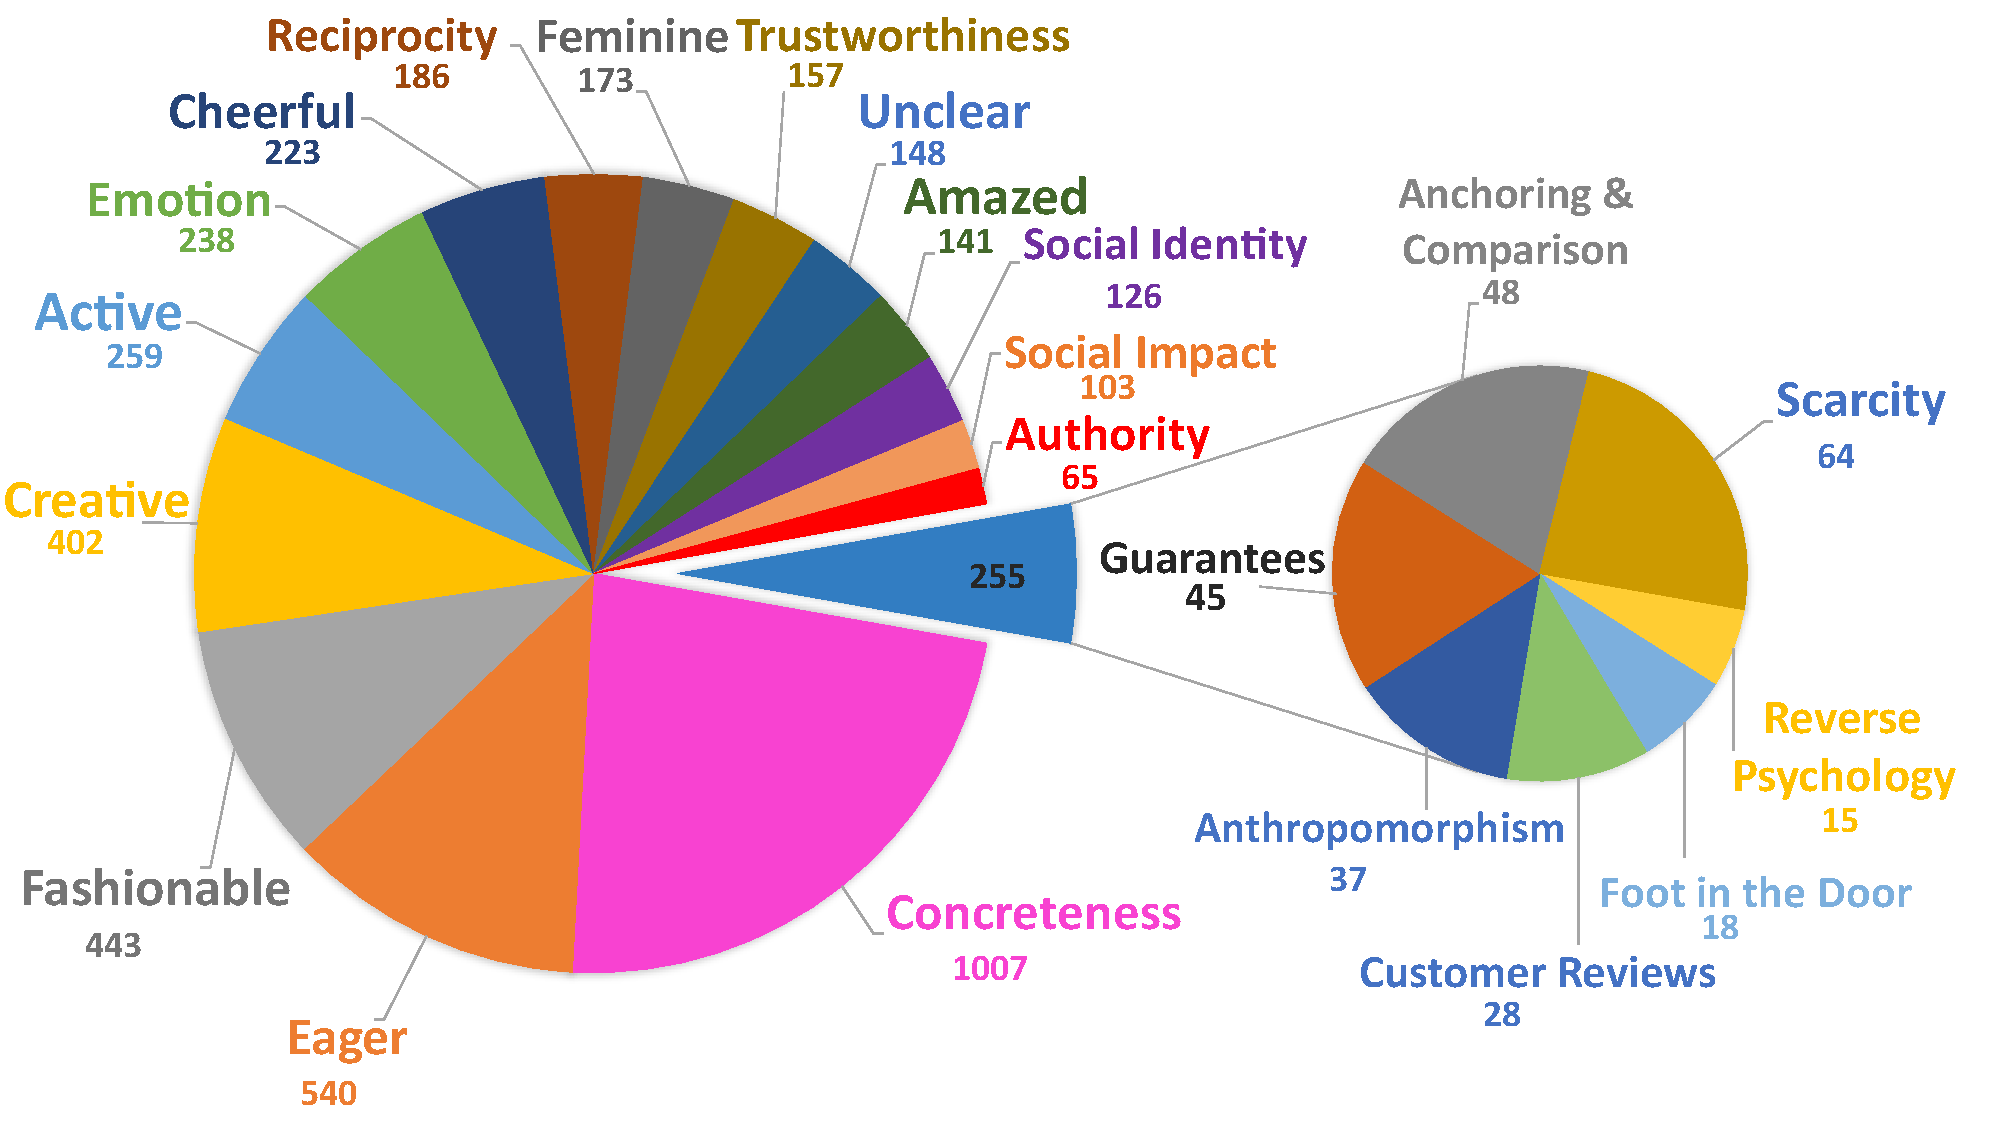
\includegraphics[scale=0.3]{images/pie_chart.pdf}
        \caption{Distribution of Persuasion Strategies in the image persuasion strategy dataset. The top-3 strategies are Concreteness, Eager, and Fashionable. \small}
        \label{fig:persuasion-strategies-distribution}
        % \vspace{-4mm}
    \end{figure}


\subsection{Persuasion Strategy Dataset For Image Advertisements}

To annotate persuasion strategies on image advertisements, we leverage raw images from the Pitts Ads dataset. It contains 64,832 image ads with labels of topics, sentiments, symbolic references (\textit{e.g.} dove symbolizing peace), and reasoning the ad provides to its viewers (see Fig~\ref{fig:preds-sup} for a few examples). The dataset had ads spanning multiple industries, products, services, and also contained public service announcements. Through this, they presented an initial work for the task of understanding visual rhetoric in ads. Since the dataset already had a few types of labels associated with the ad images, we used active learning on a model trained in a multi-task learning fashion over the reasoning task introduced in their paper. We explain the model and then the annotation strategy followed in \S\ref{sec:Persuasion Strategy Prediction Model}. 







To commence training, we initially annotated a batch of $250$ randomly selected ad images with persuasion strategies defined in Section~\ref{tab:persuasive-strategies-list}. We recruited four research assistants to label persuasion strategies for each advertisement. Definitions and examples of different persuasion strategies were provided, together with a training session where we asked annotators to annotate a number of example images and walked them through any disagreed annotations. To assess the reliability of the annotated labels, we then asked them to annotate the same 500 images and computed Cohen's Kappa statistic to measure inter-rater reliability. We obtained an average score of 0.55. The theoretical maximum of Kappa, given the unequal distribution, is 0.76. In such cases, Cohen \cite{cohen1960coefficient} suggested that one should divide kappa by its maximum value $\mathbf{k}/\mathbf{k_{max}}$, which comes out to be 0.72. This is a \textit{substantial} agreement. Further, to maintain labeling consistency, each image was double annotated, with all discrepancies resolved by an intervention of the third annotator using a majority vote. 


The assistants were asked to label each image with no more than 3 strategies. If an image had more than 3 strategies, they were asked to list the top 3 strategies according to the area covered by the pixels depicting that strategy. In total, we label 3000 ad-images with their persuasion strategies; and the number of samples in train, val, and test split are 2500, 250, and 250, respectively\footnote{Table~\ref{table:strategy-train-test-val-stats} shows the detailed distribution of the number of strategies in ads}. Fig.~\ref{fig:persuasion-strategies-distribution} presents the distribution of persuasion strategies in the dataset. It is observed that concreteness is the most used strategy in the dataset, followed by eagerness and fashion. The average number of strategies in an ad is 1.49, and the standard deviation is 0.592. We find that scarcity (92.2\%), guarantees (91.1\%), reciprocity (84.4\%), social identity (83.3\%), and cheerful (83\%), %and anchoring and comparison (77.1\%), trustworthiness (75.8\%), social proof (75\%),  amazed (73.1\%) and concreteness (70.3\%) 
are the top 5 strategies, which occur in groups of 2 or 3. We observe that the co-occurrence of these strategies is due to the fact that many of them cover only a single modality (\textit{i.e.}, text or visual), leaving the other modality free for a different strategy. For example, concreteness is often indicated by illustrating points in text, while the visual modality is free for depicting, say, emotion. See Fig.~\ref{fig:segmented image} for an example, where the image depicting \textit{Authority} also has concreteness strategy in it. Similarly, feminine emotion is also depicted in Fig.~\ref{fig:footwear-strategies}, along with concreteness.


\begin{figure*}[!h]
    % \vspace{-4mm}
    \centering
    \begin{subfigure}[b]{0.4\textwidth}
        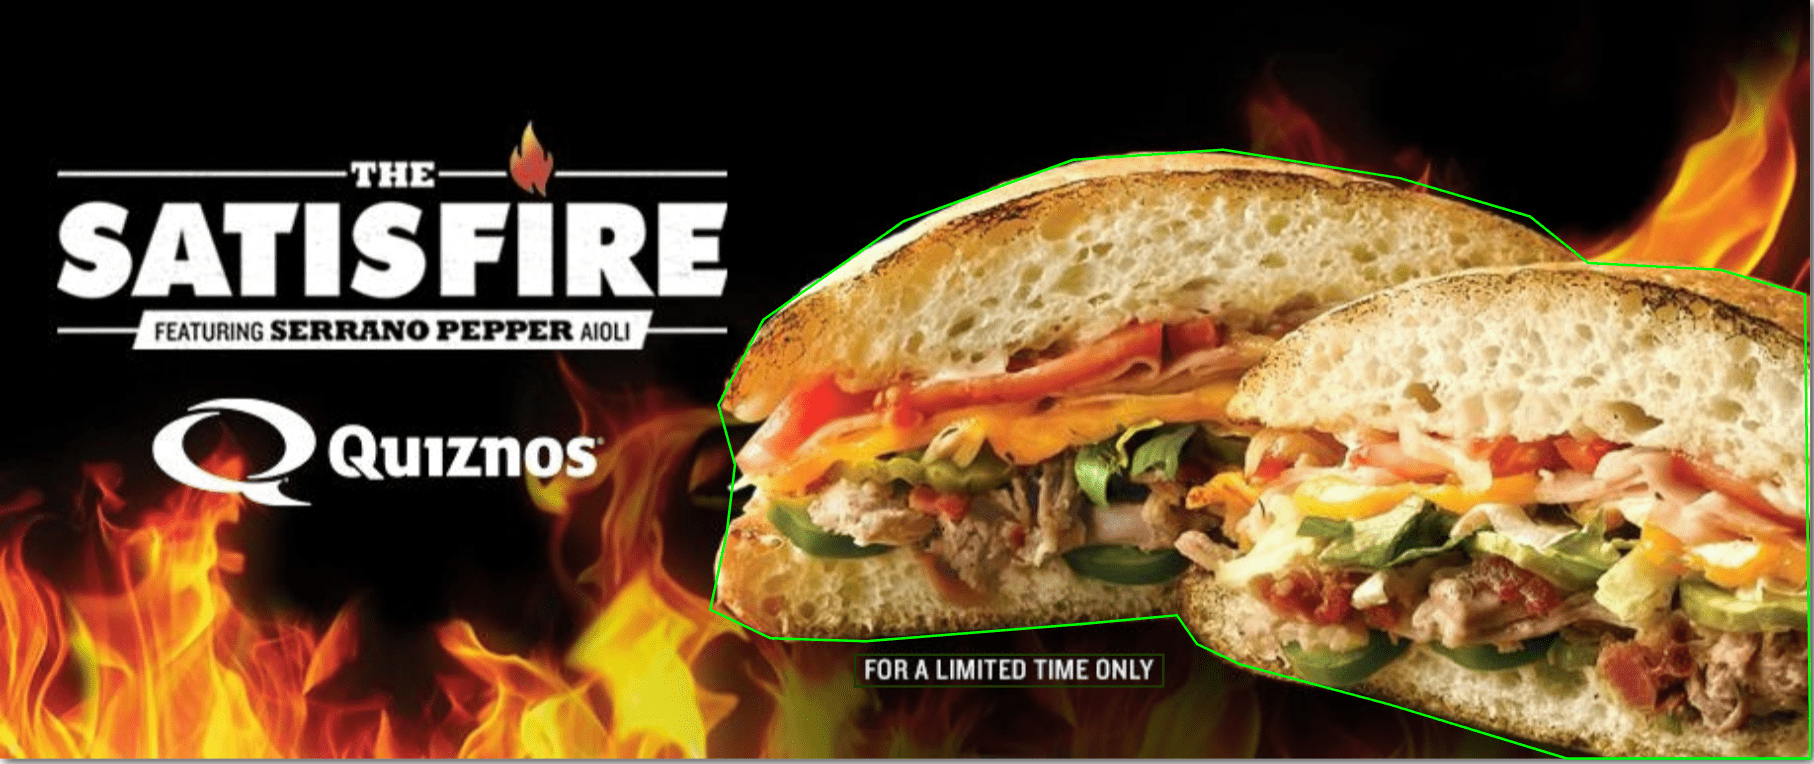
\includegraphics[scale=0.2]{images/Image1.png}
    \end{subfigure}
    \begin{subfigure}[b]{0.4\textwidth}
        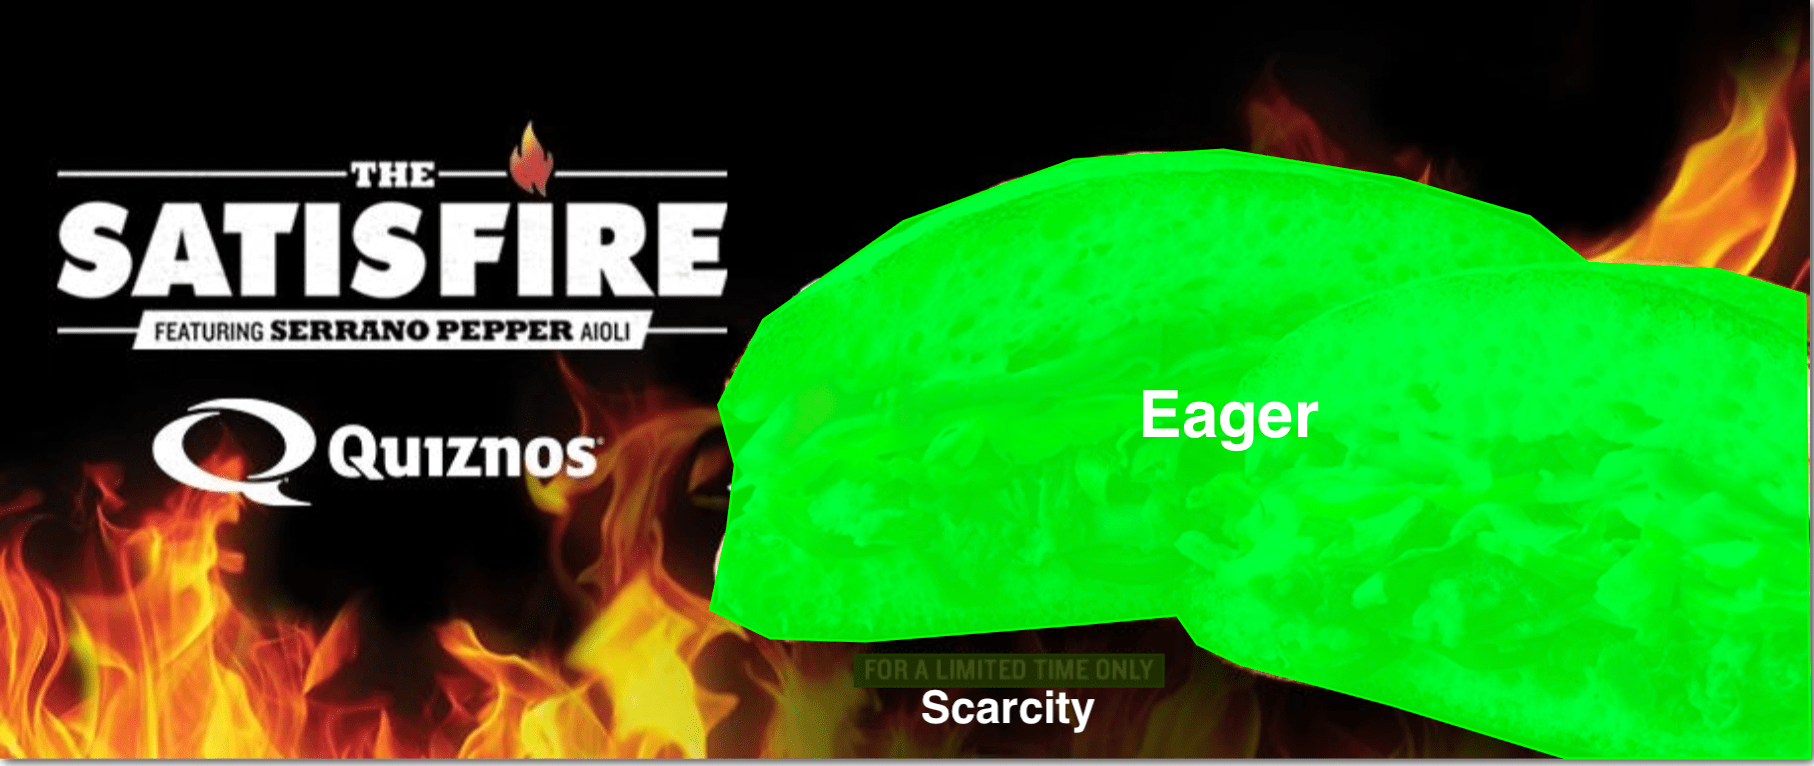
\includegraphics[scale=0.2]{images/Image1_Segment.png}



    \end{subfigure}
     \begin{subfigure}[b]{0.245\textwidth}
         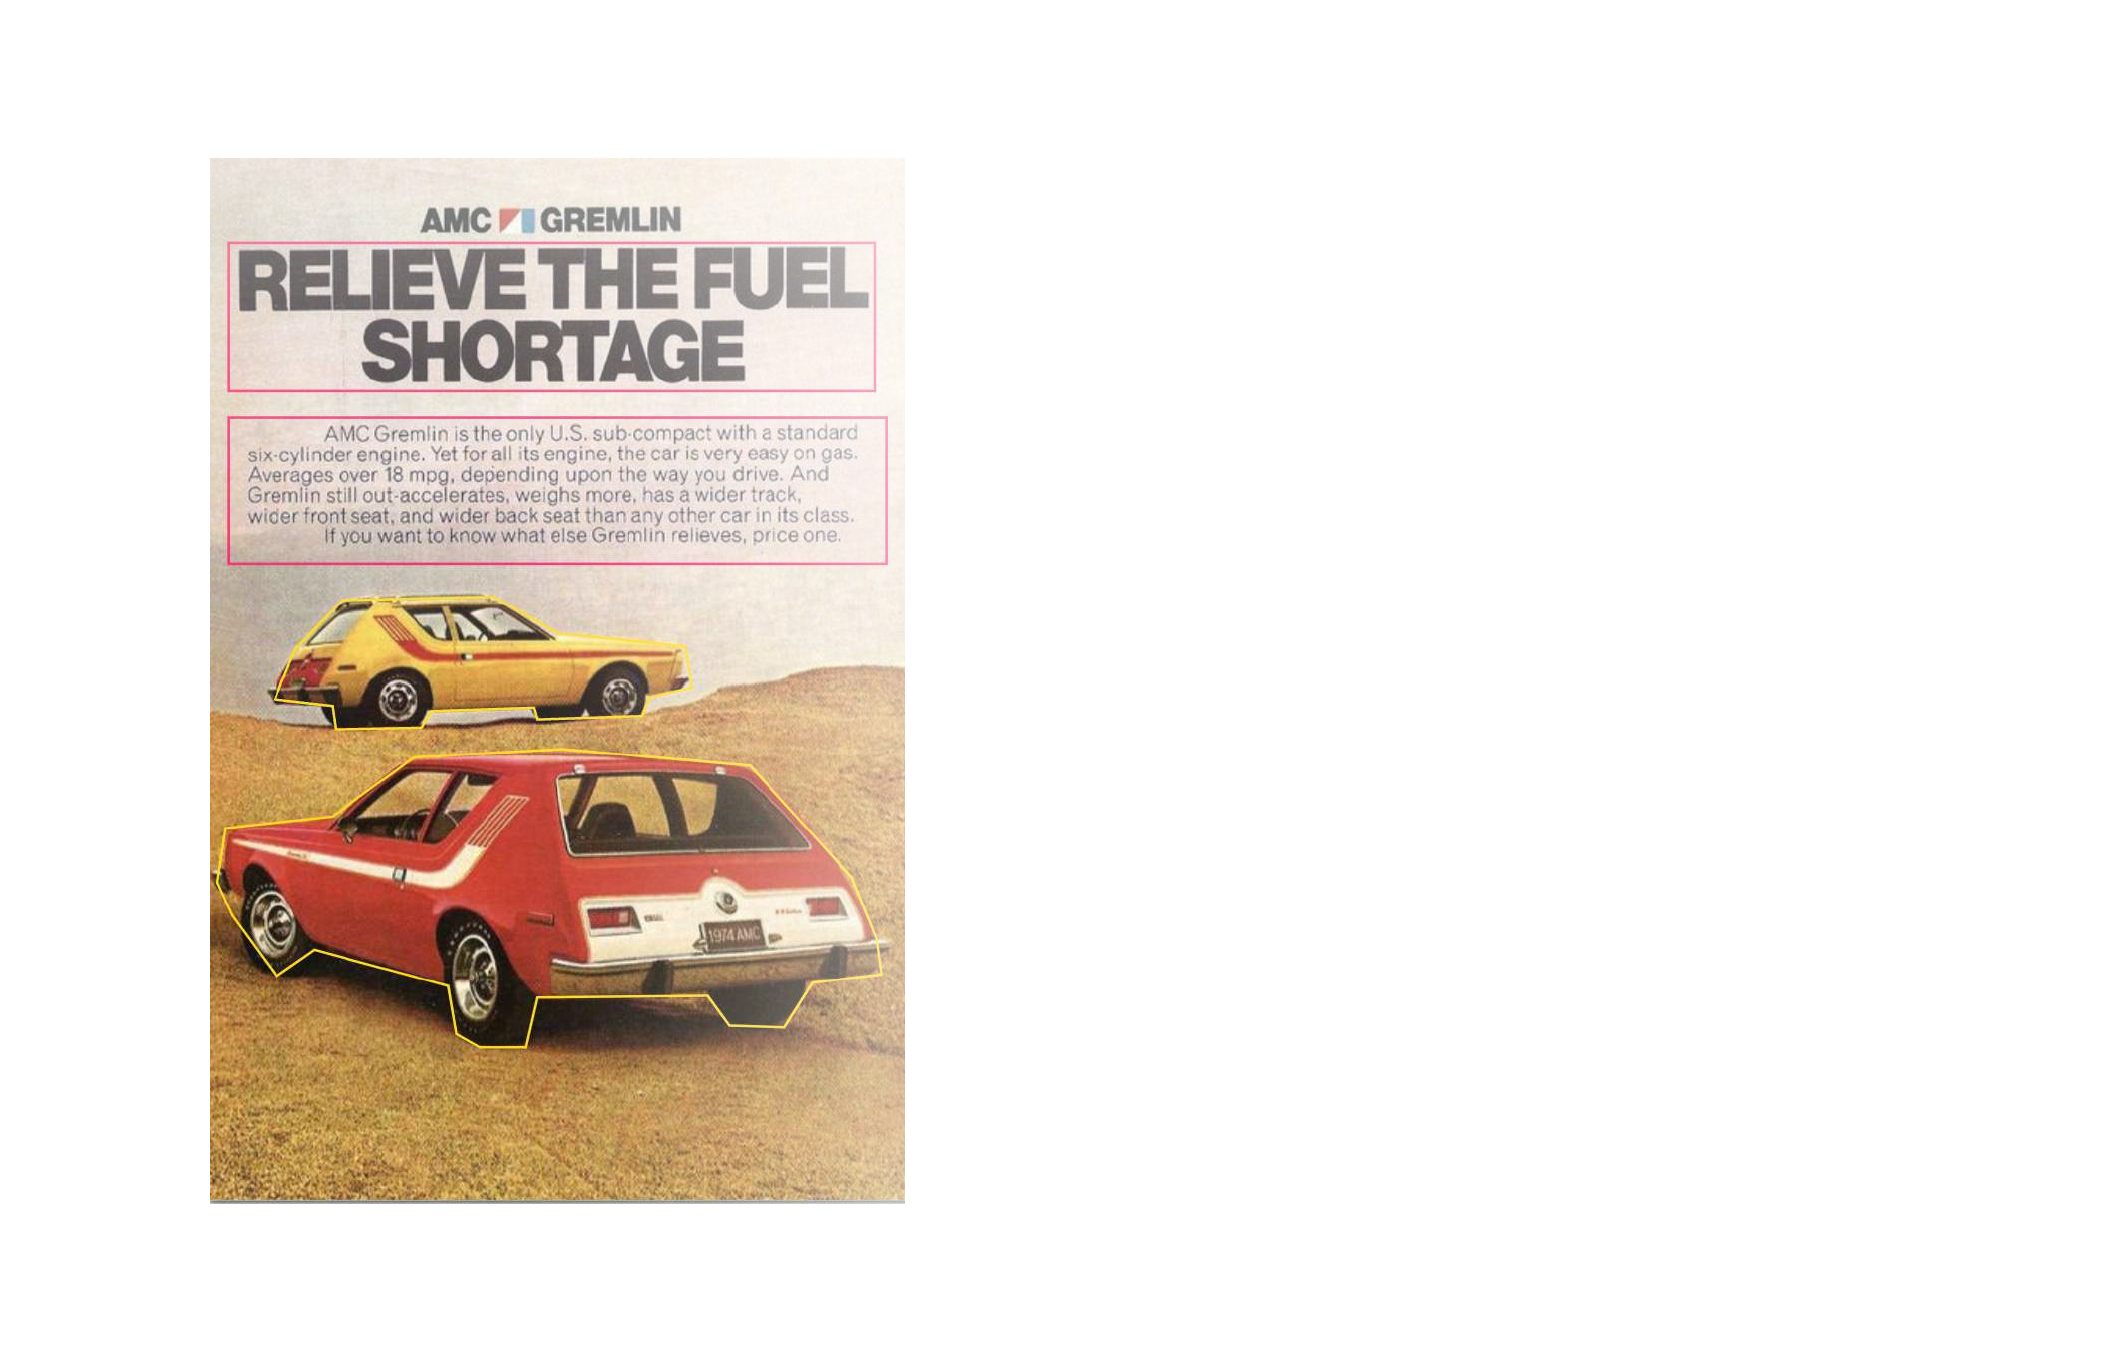
\includegraphics[scale=0.22]{images/fuel-shortage-original.pdf}
     \end{subfigure}
     \begin{subfigure}[b]{0.245\textwidth}
         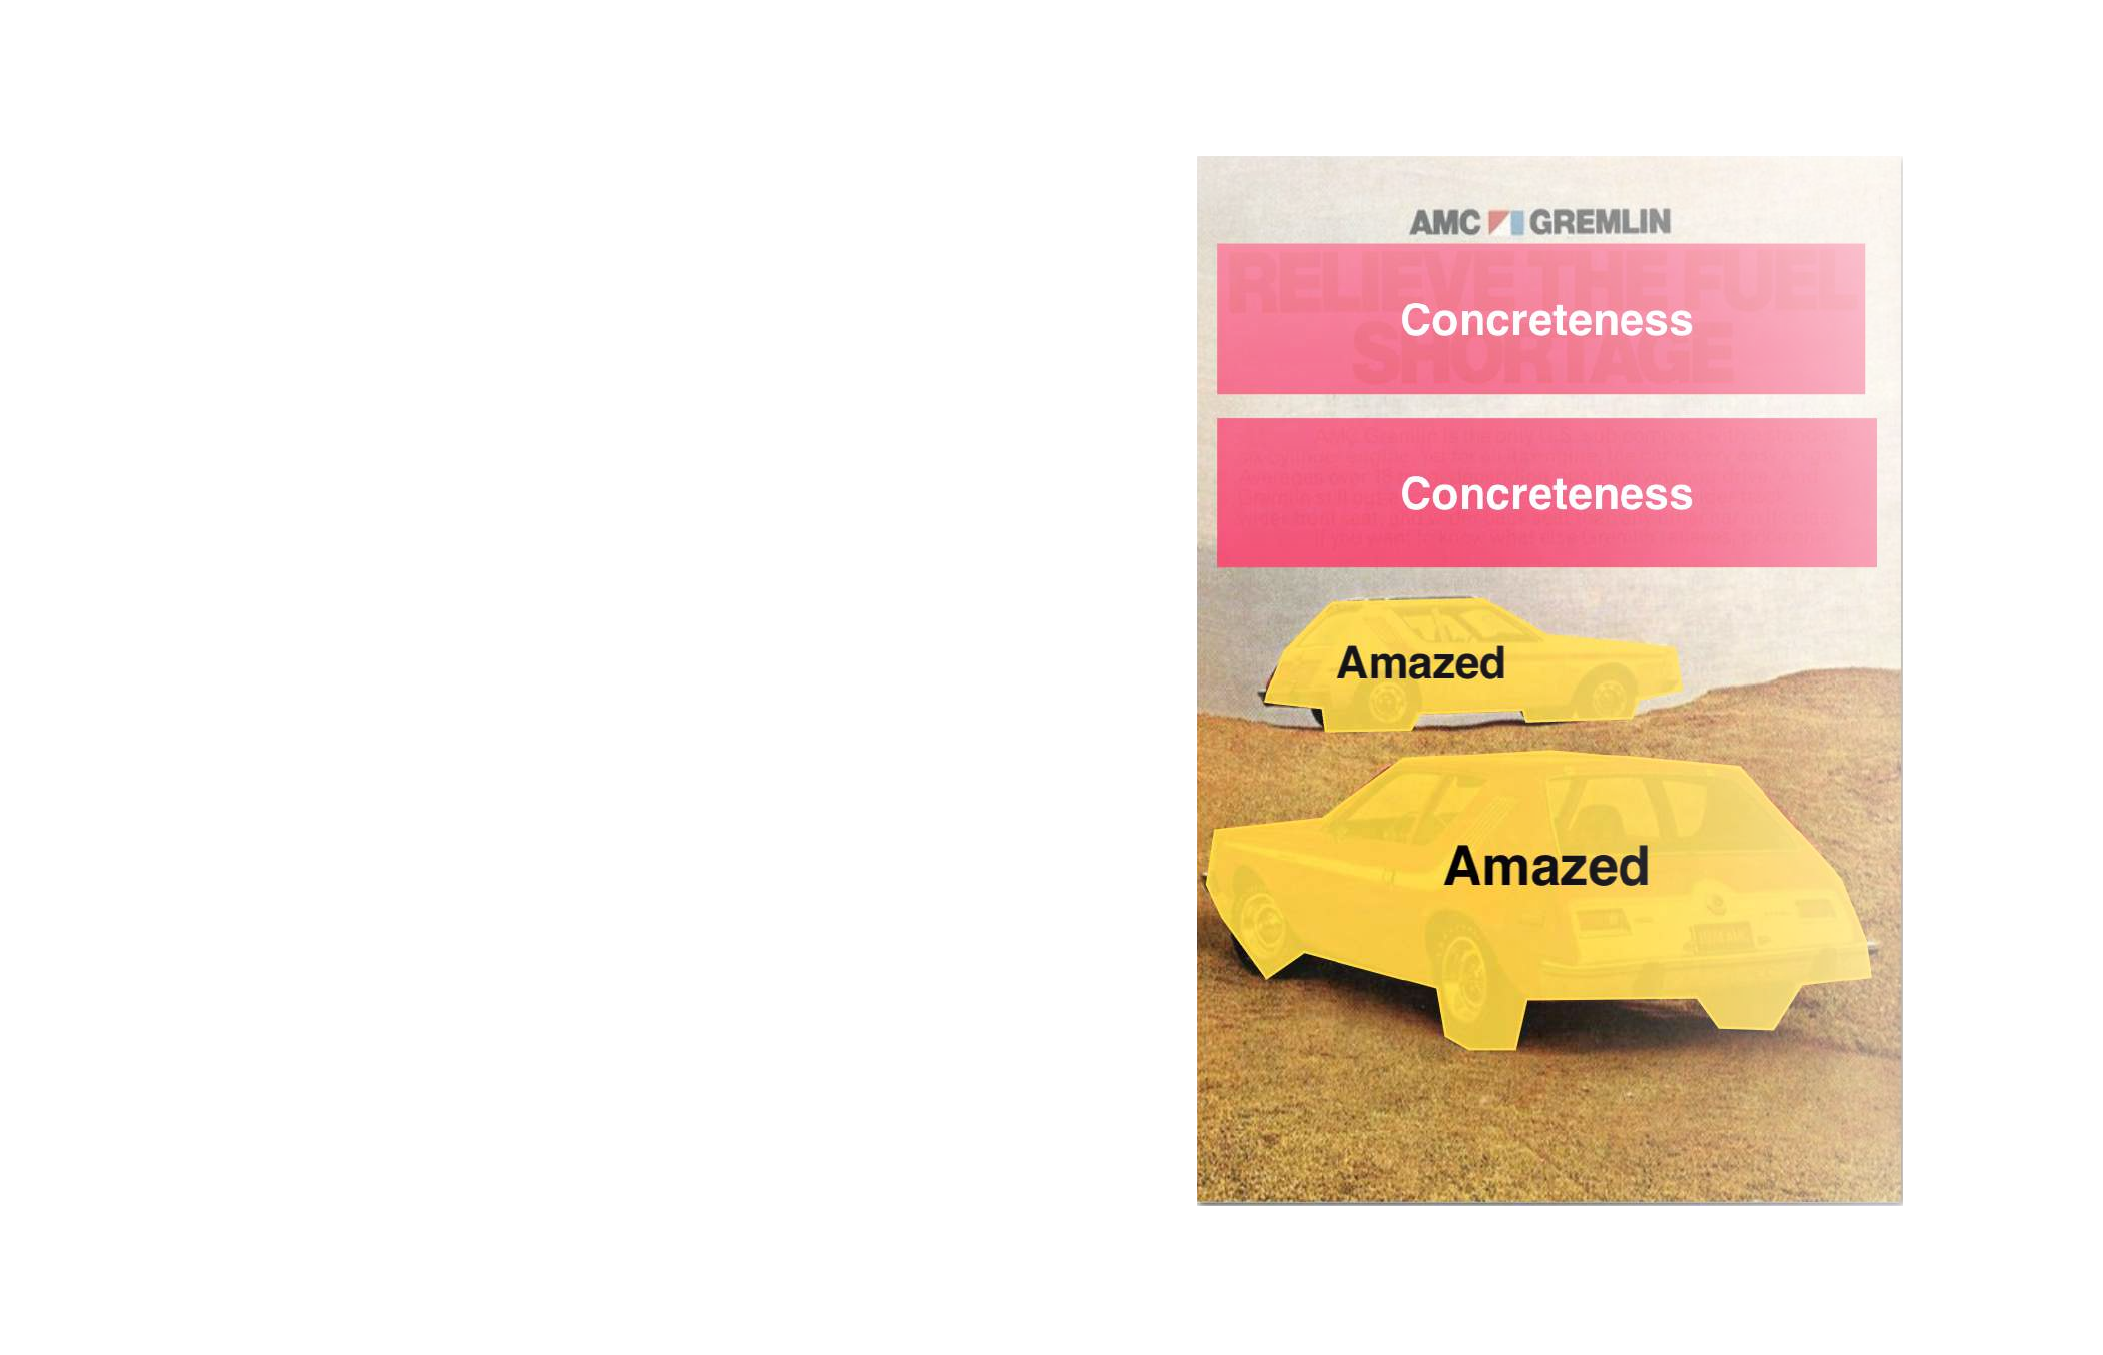
\includegraphics[scale=0.22]{images/fuel-shortage-segmented.pdf}
     \end{subfigure}
     \begin{subfigure}[b]{0.24\textwidth}
         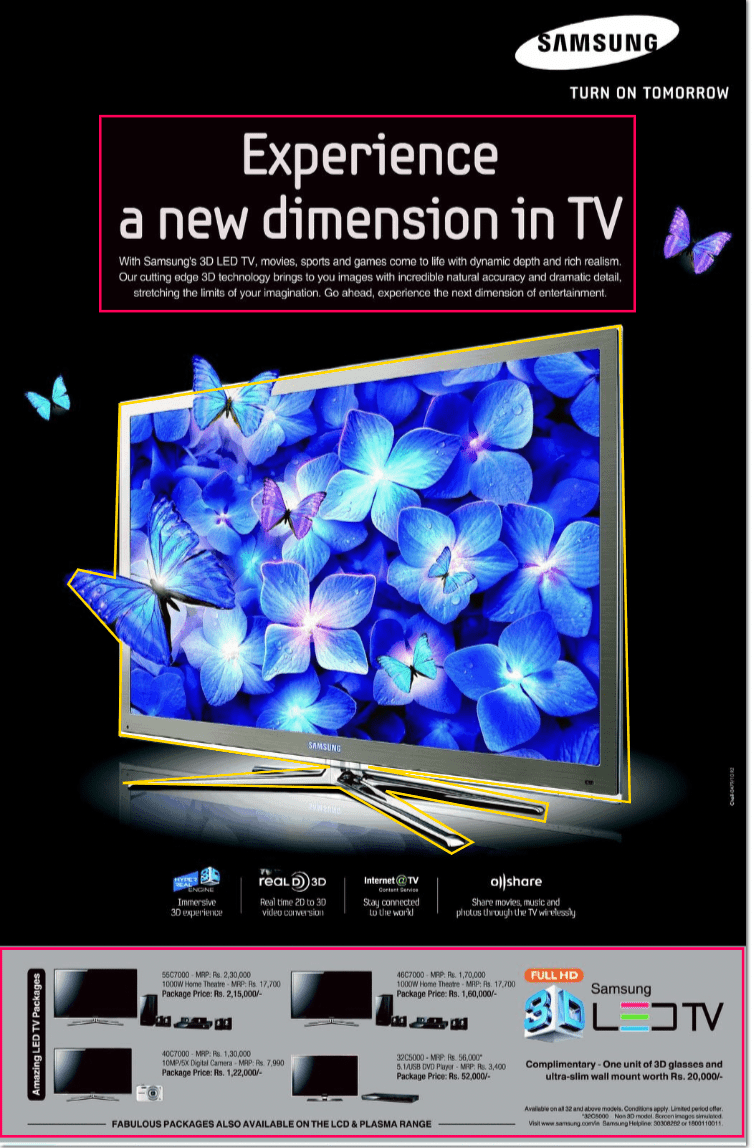
\includegraphics[scale=0.22]{images/Image2.png}
     \end{subfigure}
     \begin{subfigure}[b]{0.24\textwidth}
         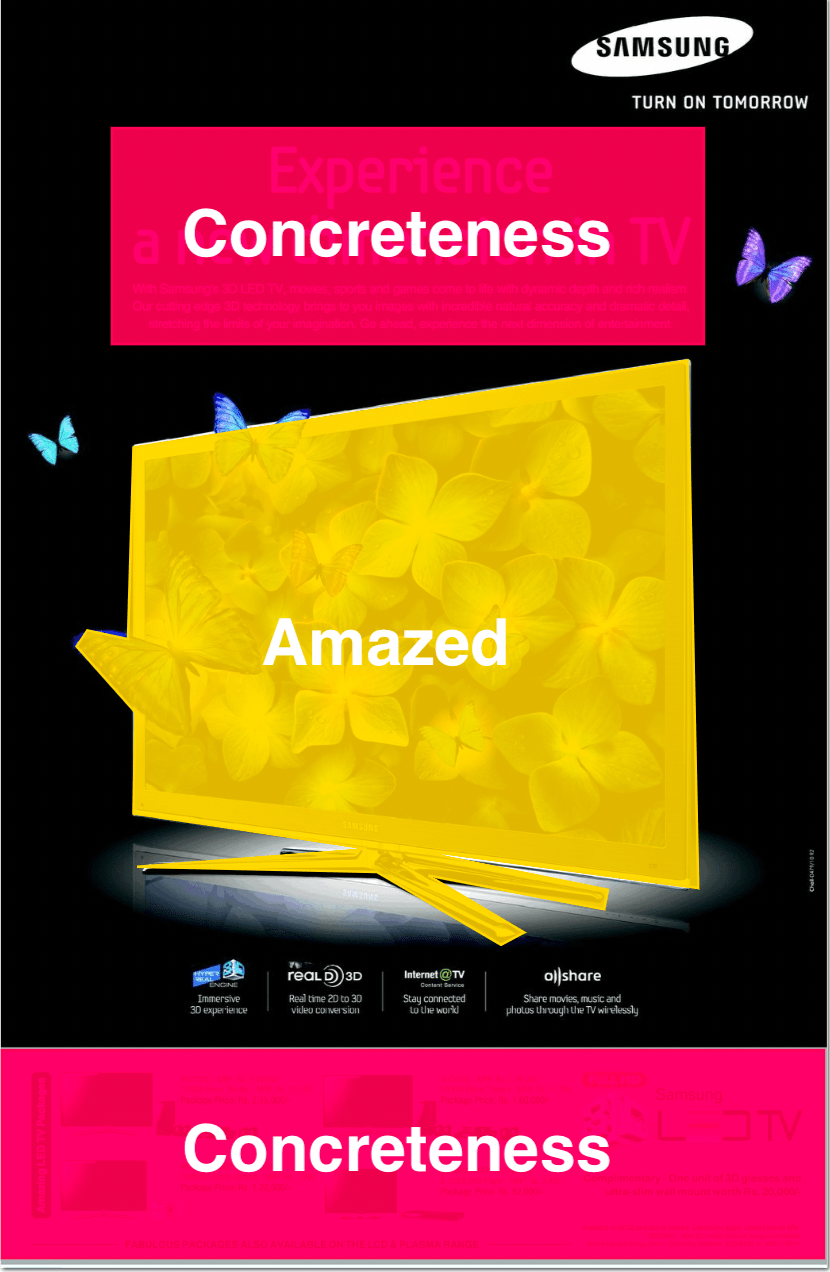
\includegraphics[scale=0.22]{images/Image2_Segment.png}
     \end{subfigure}


    \begin{subfigure}[b]{0.24\textwidth}
        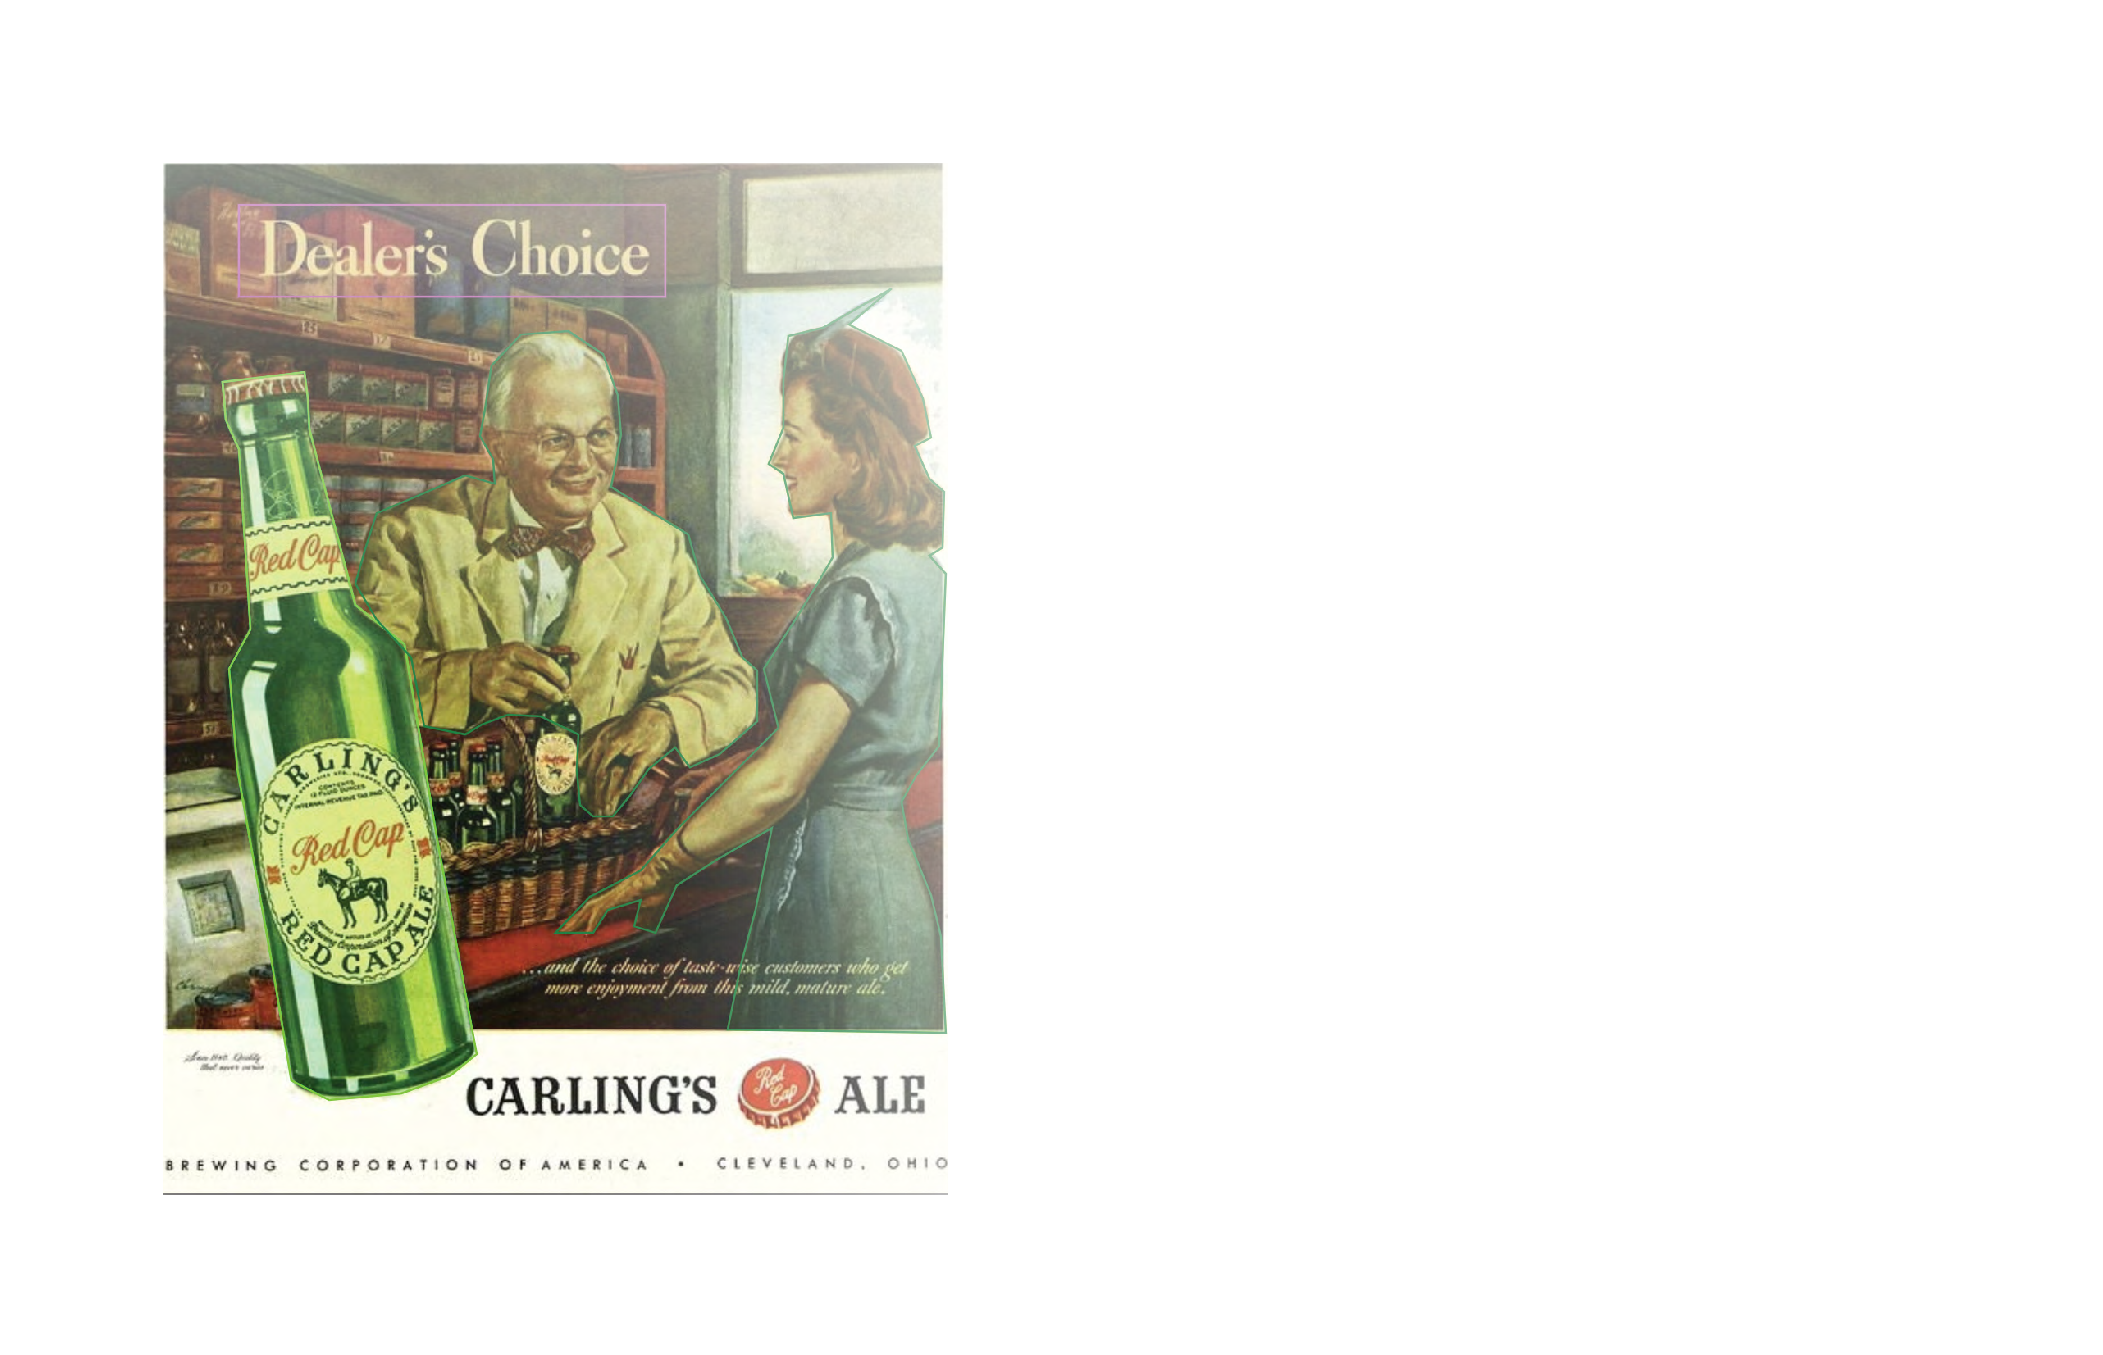
\includegraphics[scale=0.22]{images/dealer-choice-original.pdf}
    \end{subfigure}
    \begin{subfigure}[b]{0.24\textwidth}
        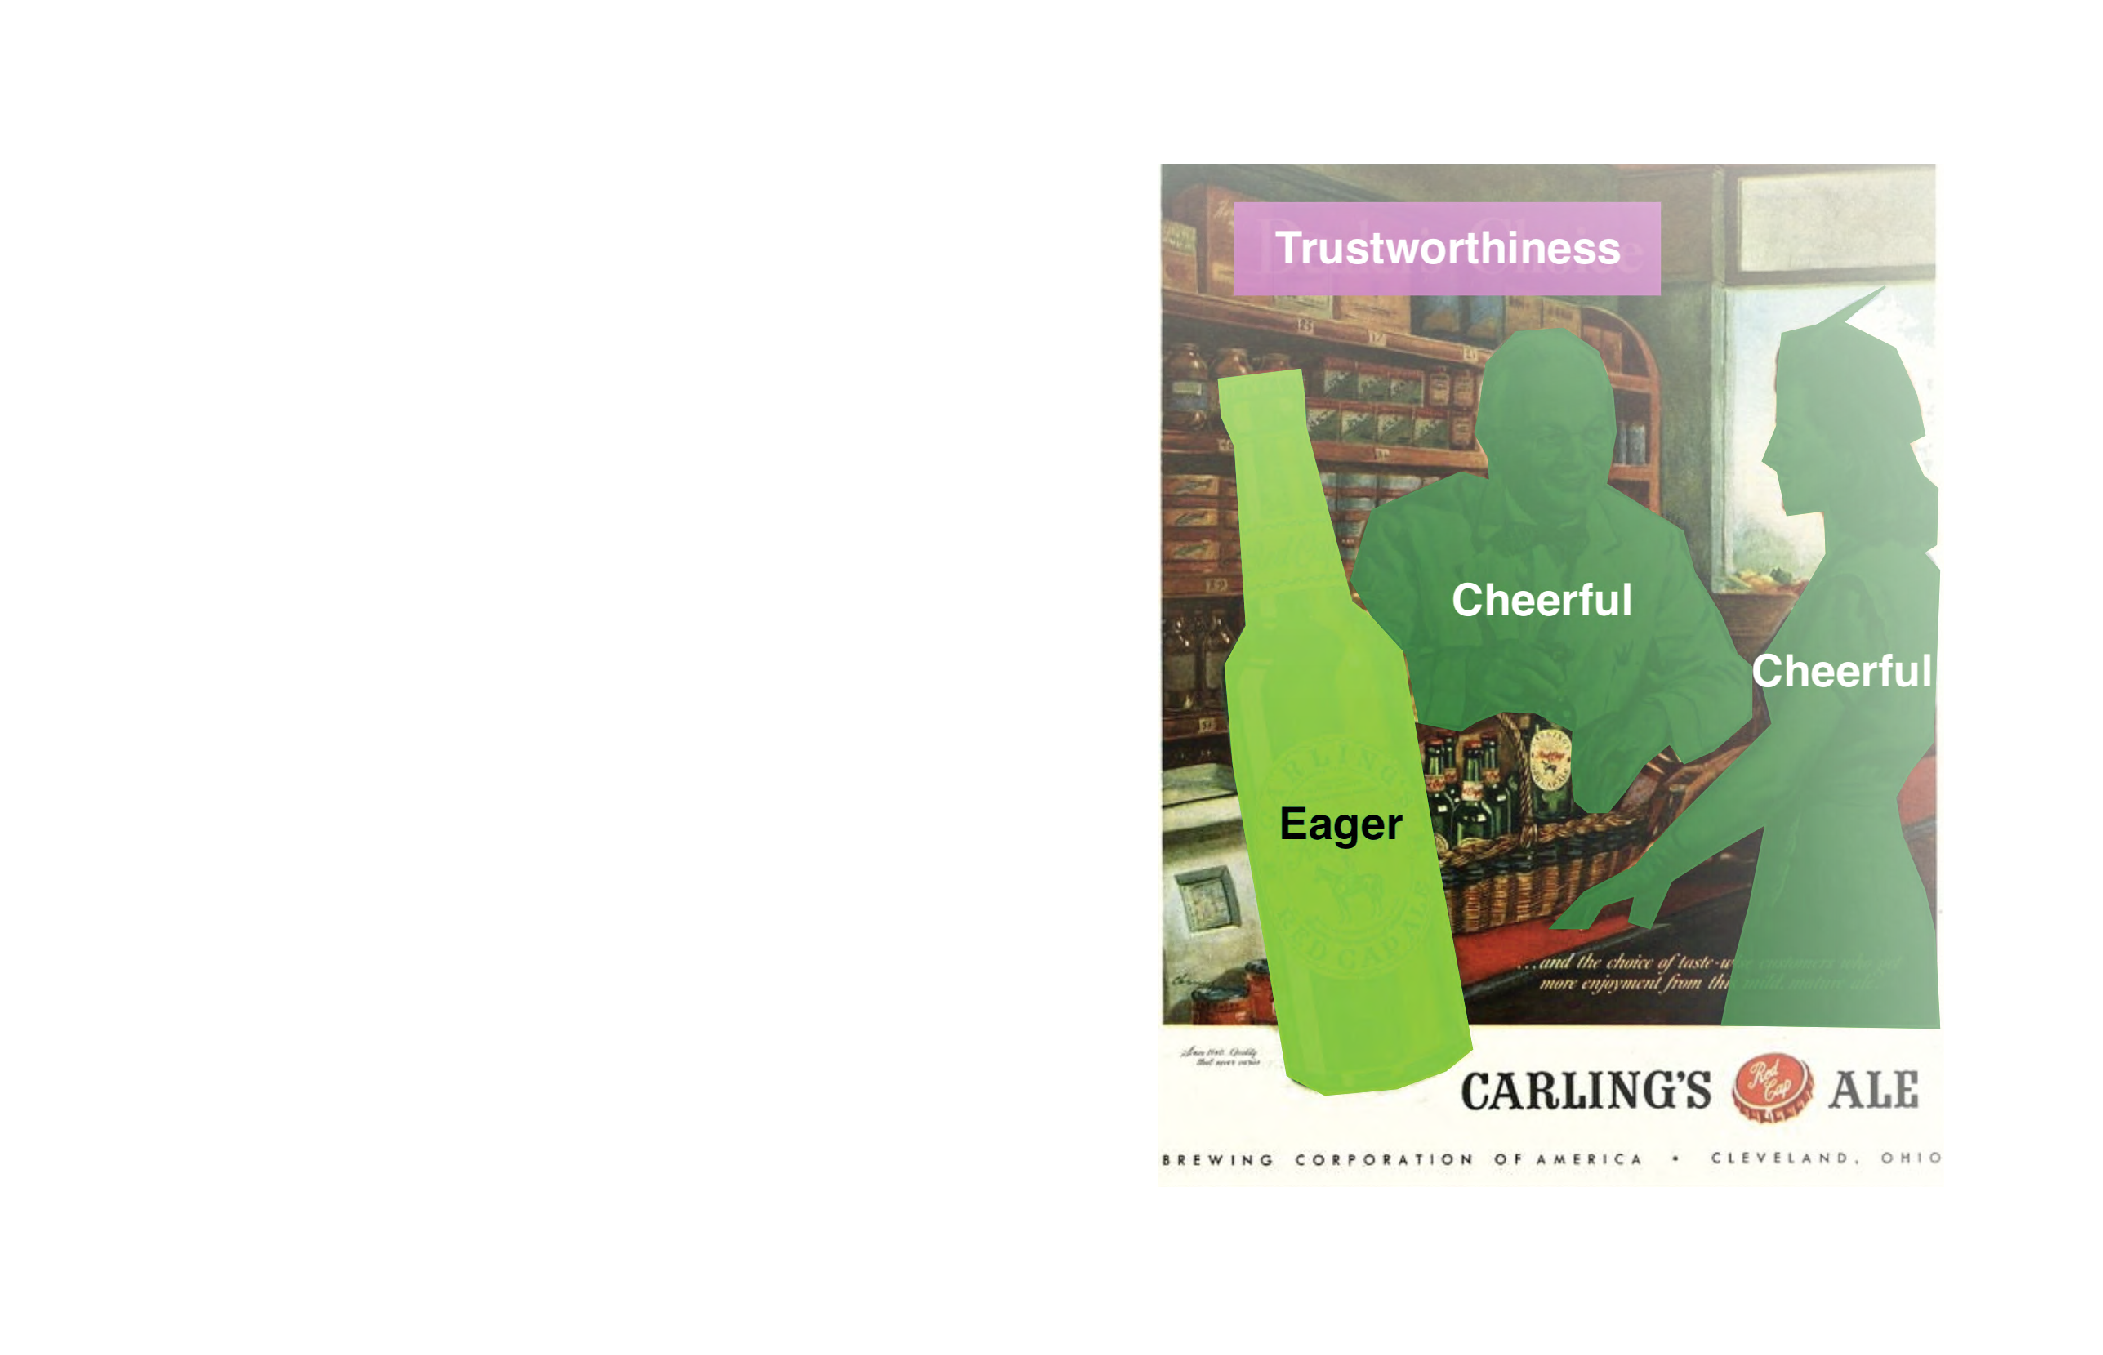
\includegraphics[scale=0.22]{images/dealer-choice-segmented.pdf}
    \end{subfigure}
     \begin{subfigure}[b]{0.24\textwidth}
         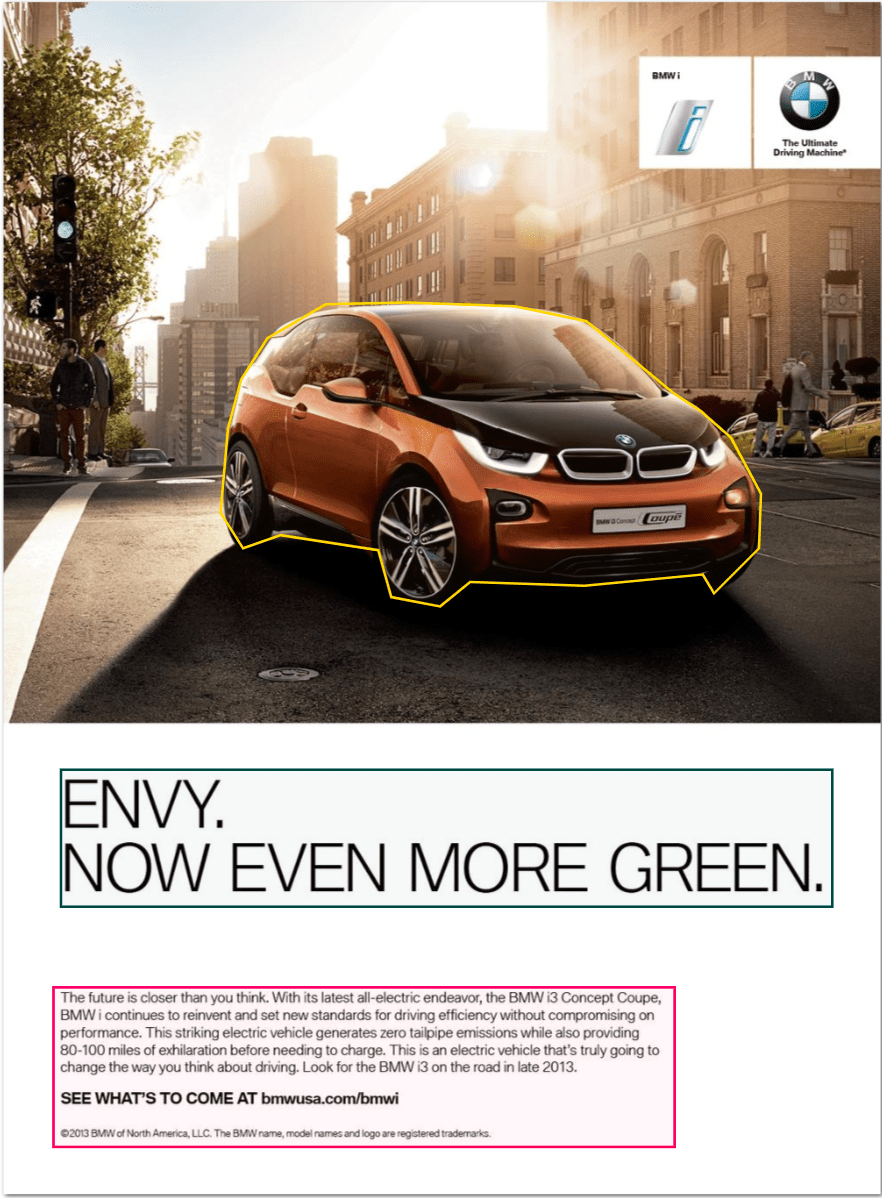
\includegraphics[scale=0.22]{images/Image3.png}
     \end{subfigure}
     \begin{subfigure}[b]{0.24\textwidth}
         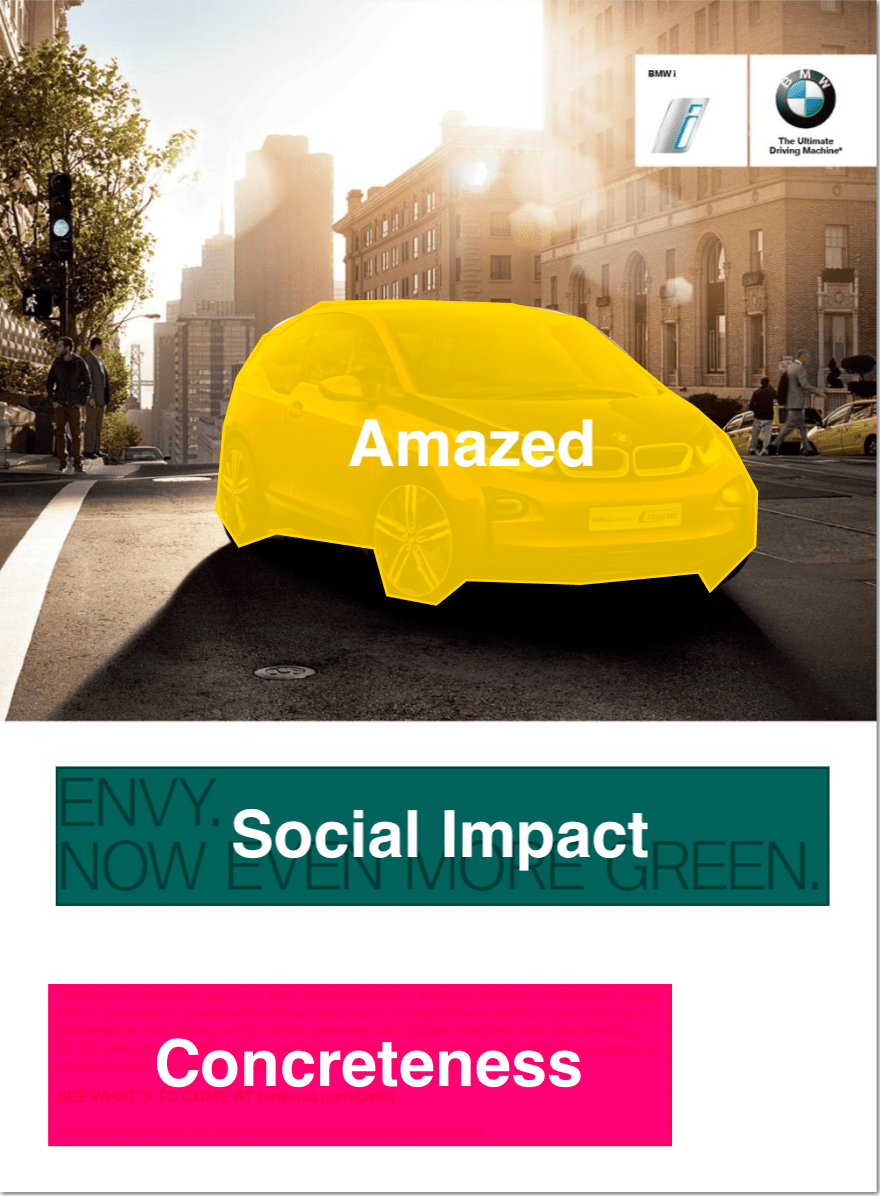
\includegraphics[scale=0.22]{images/Image3_Segment.png}
     \end{subfigure}
     
     \begin{subfigure}[b]{0.4\textwidth}
         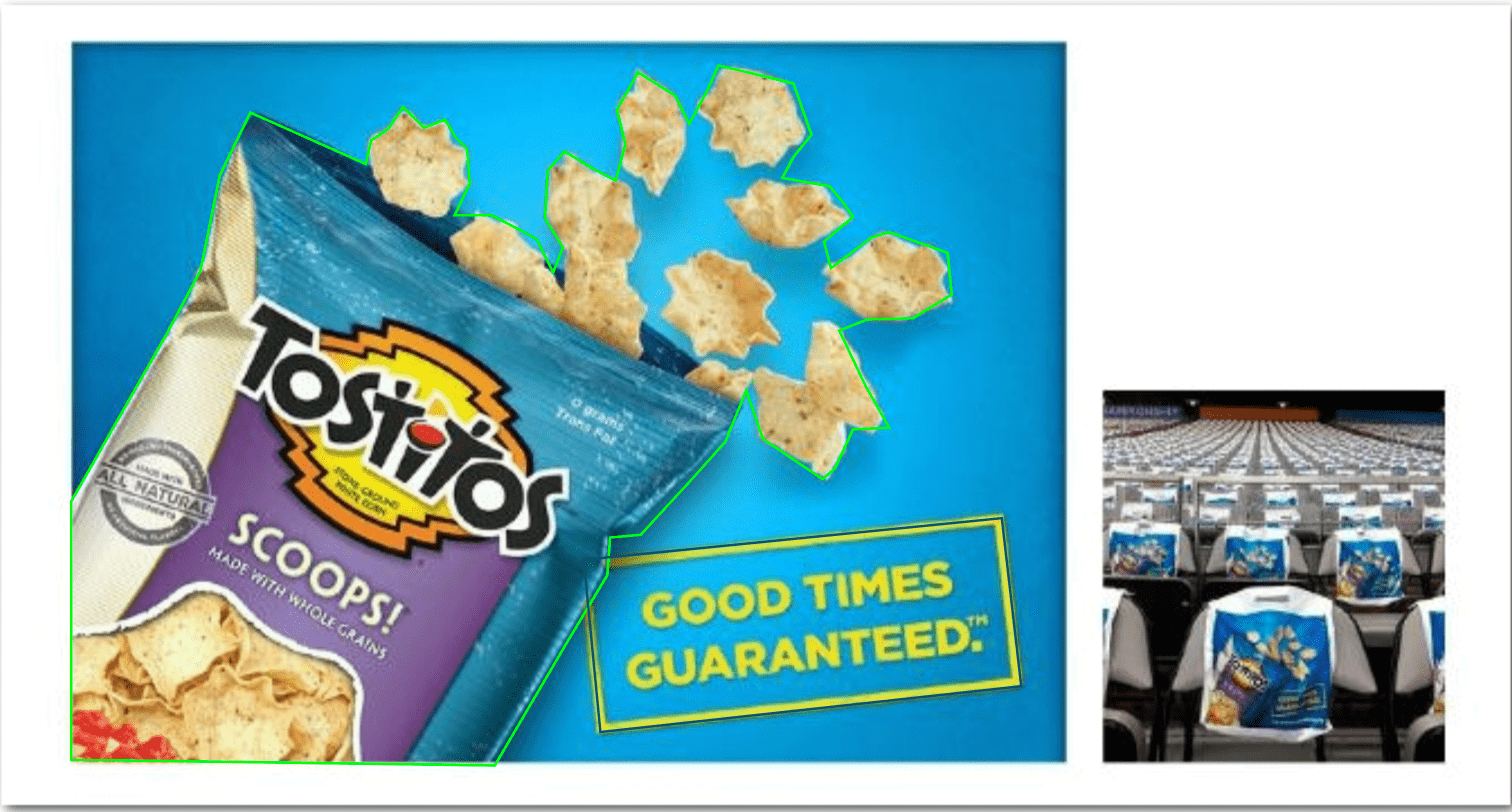
\includegraphics[scale=0.22]{images/Image4.png}
     \end{subfigure}
     \begin{subfigure}[b]{0.4\textwidth}
         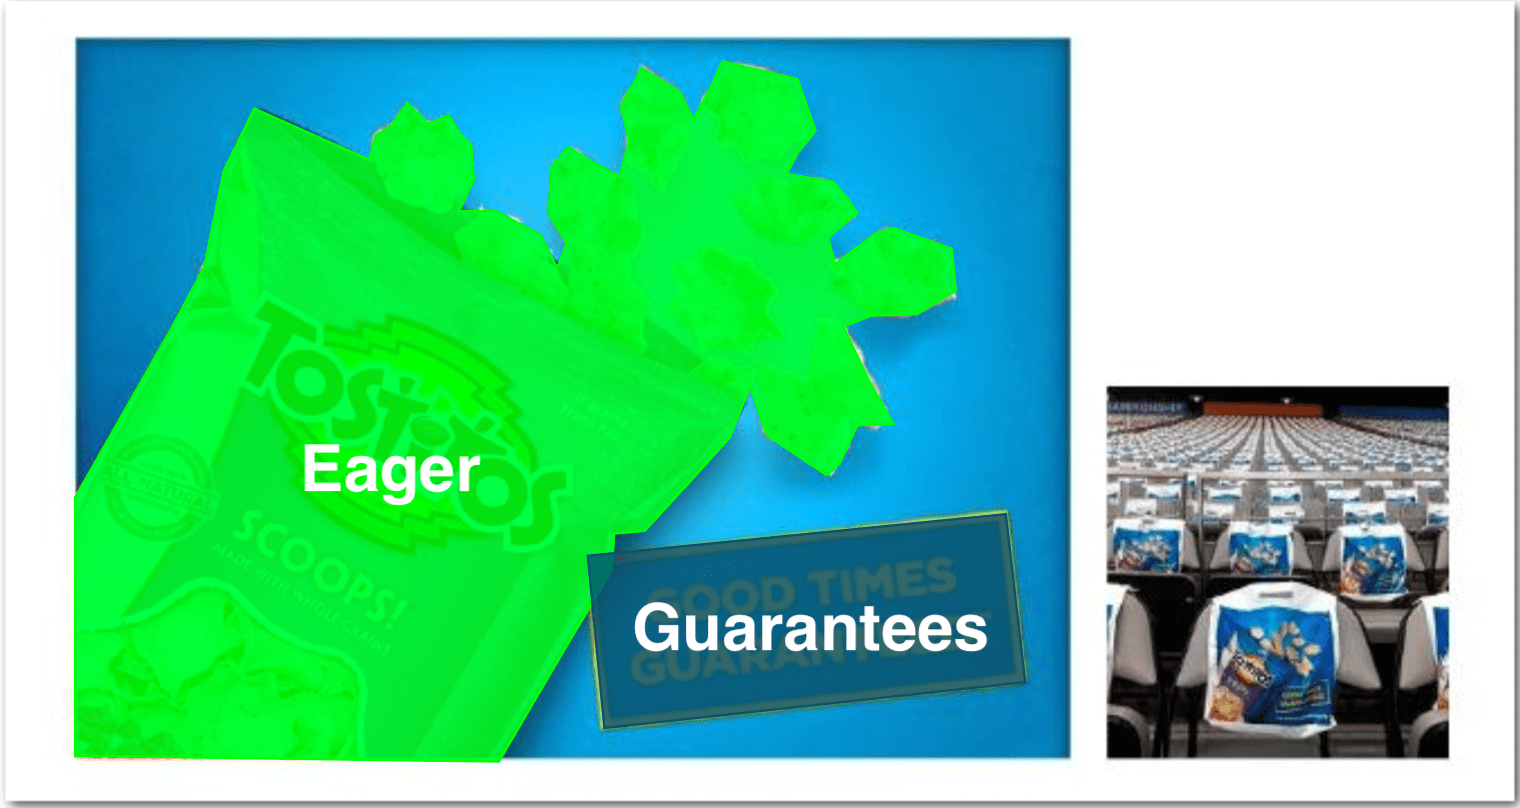
\includegraphics[scale=0.22]{images/Image4_Segment.png}
     \end{subfigure}
     
    \caption{\small \label{fig:segmented image} Image with a segmentation mask depicting the strategies \textit{Emotion:Cheerful}, \textit{Emotion:Eager} and \textit{Trustworthiness}.}
    % \vspace{-4mm}
\end{figure*}







Next, we calculate the Dice correlation coefficient\footnote{The Dice Coefficient is defined as: \; \(2*|X \cap Y|\: / \:(|X|+|Y|)\), where X and Y are two sets; a set with vertical bars on either side refers to the cardinality of the set, i.e. the number of elements in that set; and \(\cap\)  refers to the intersection of two sets.} statistics for pairs of co-occurring persuasion strategies. The top-5 pairs are eager-concreteness (0.27), scarcity-reciprocity (0.25), eager-cheerful (0.19), amazed-concreteness (0.17), and eager-reciprocity (0.17). We find that these correlation values are not particularly high since marketers seldom use \textit{common pairings} of messaging strategies to market their products. The visual part mostly shows eager strategy in ads; therefore, we find that the text modality becomes free to show other strategies. That is why primarily text-based concreteness, cheerfulness, and reciprocity strategies are present with the visual-based eager strategy in the text modality. Also, primarily vision-based amazement, eagerness, and scarcity (short-text) strategies co-occur with text-based reciprocity and concreteness (\textit{e.g.}, Fig.~\ref{fig:footwear-strategies}).


\begin{figure*}
    \centering
    \begin{subfigure}[b]{0.3\textwidth}
         \centering
         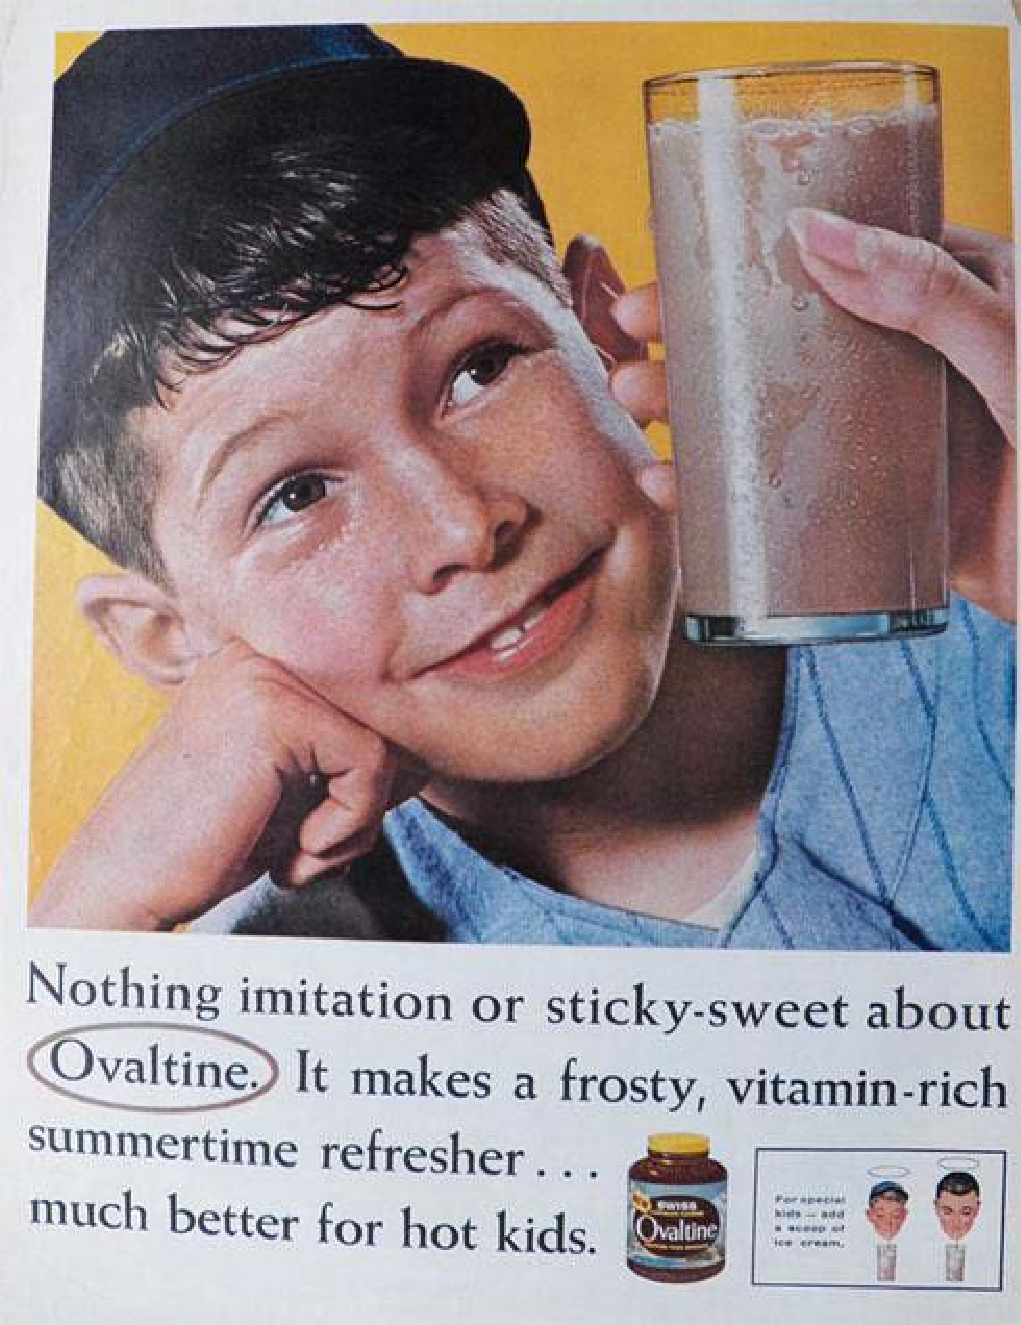
\includegraphics[width=\textwidth,scale=0.6]{images/humans_concreteness_img1.pdf}
         \caption{}
         
     \end{subfigure}
     \begin{subfigure}[b]{0.3\textwidth}
         \centering
         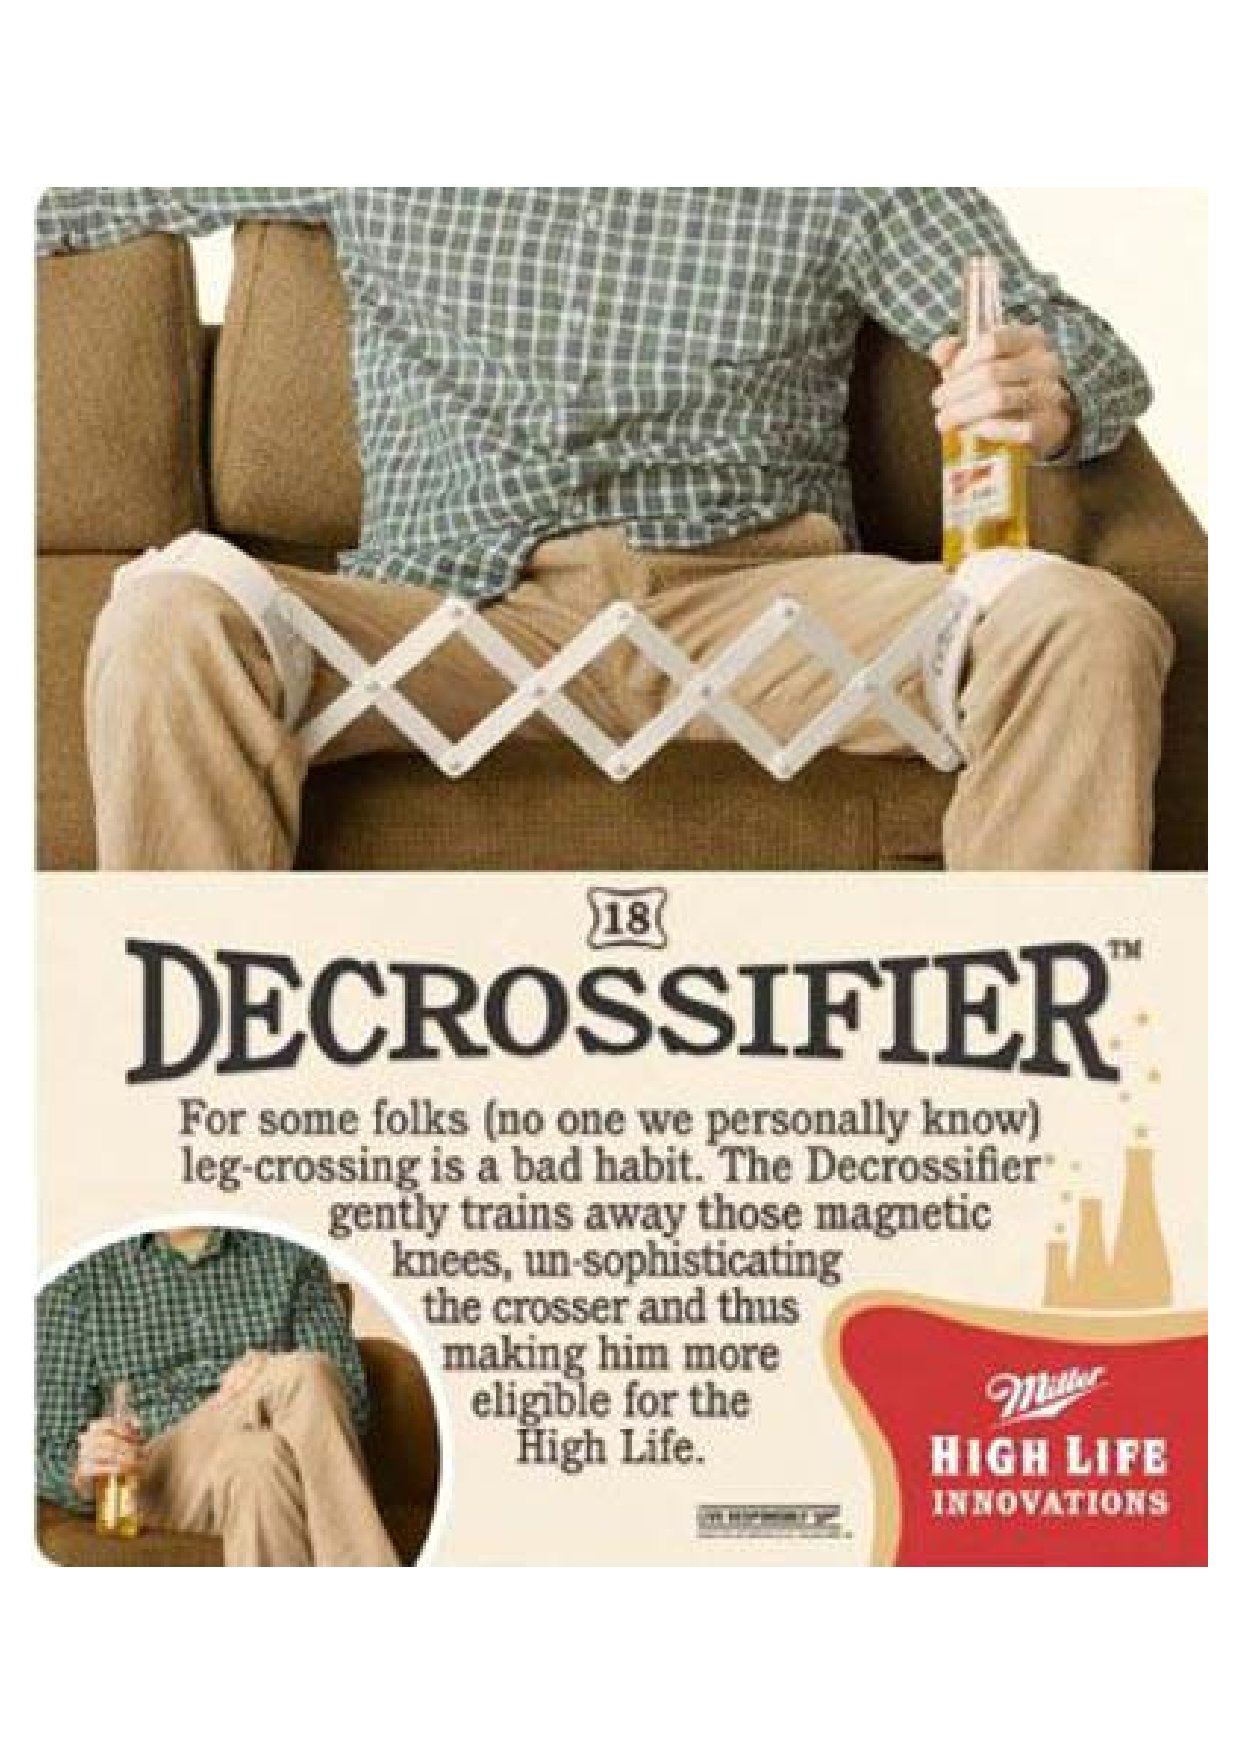
\includegraphics[width=\textwidth,scale=0.5]{images/humans_concreteness_img2.pdf}
         \caption{}
         
     \end{subfigure}
     \begin{subfigure}[b]{0.3\textwidth}
         \centering
         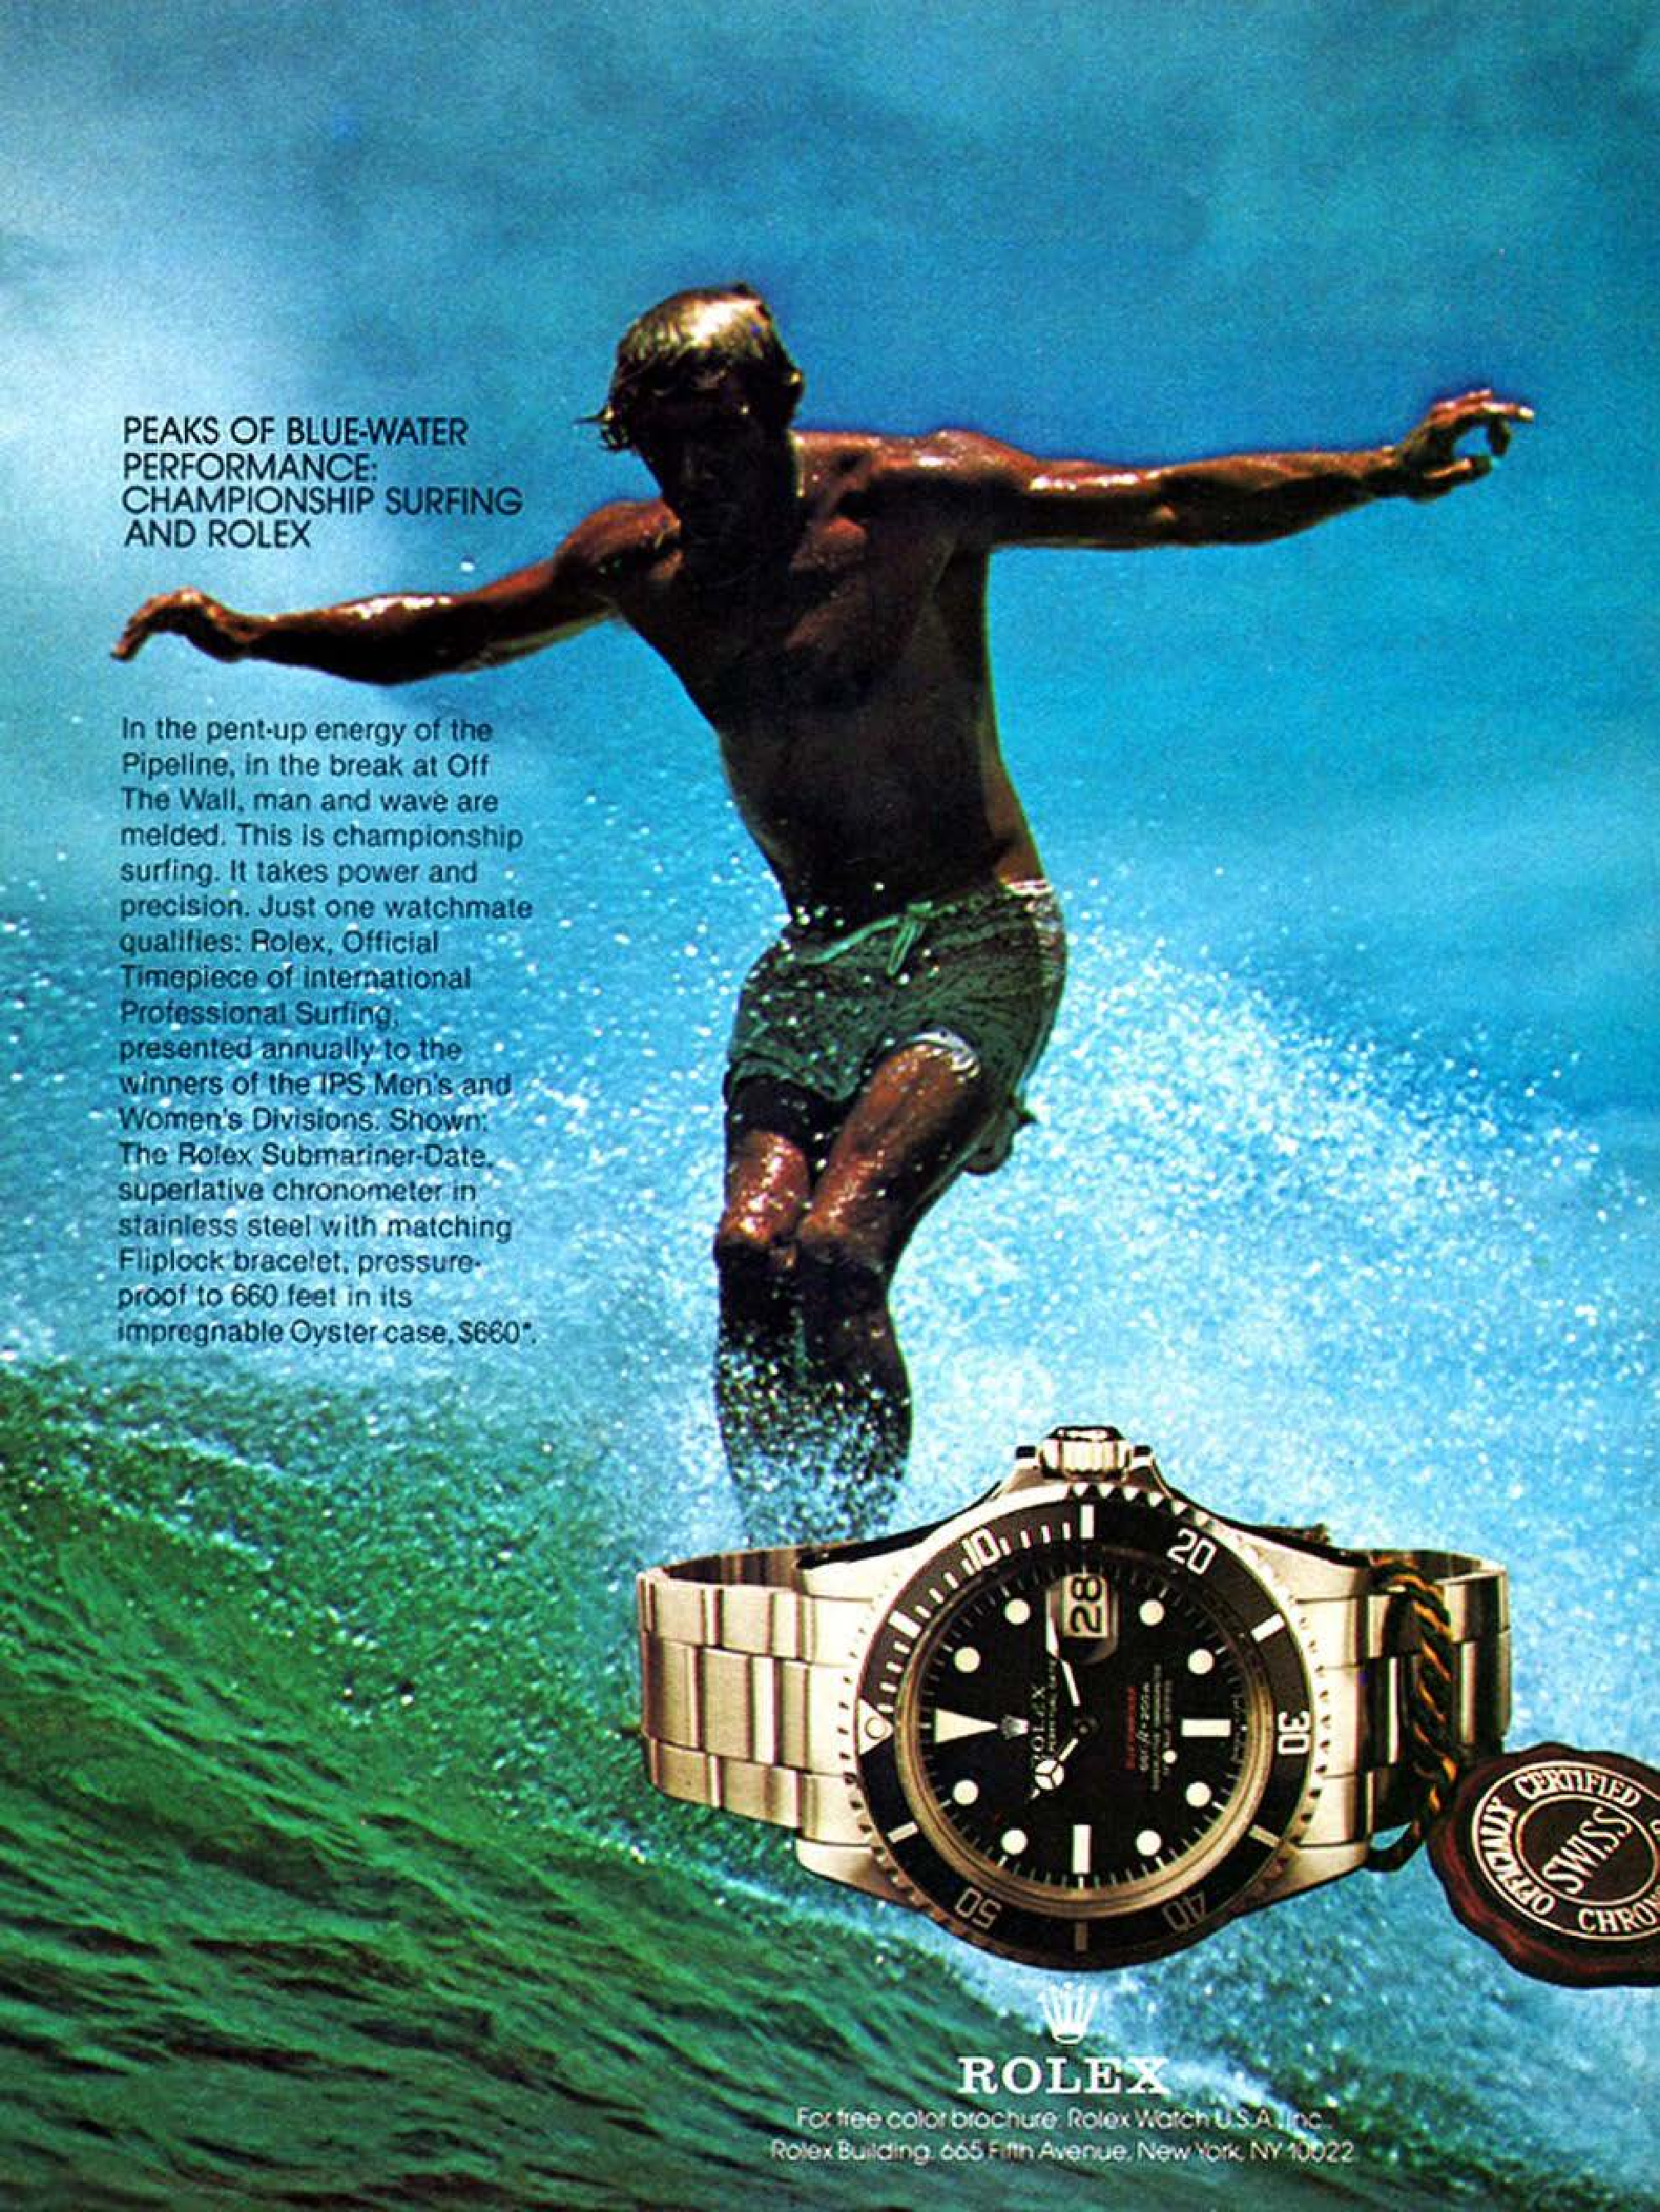
\includegraphics[width=\textwidth,scale=1.0]{images/humans_concreteness_img3.pdf}
         \caption{}
         
     \end{subfigure}
    \caption{Advertisements containing humans and concreteness}
    \label{fig:humans_concreteness-ads}
\end{figure*}




\begin{figure}[h]
        \centering
        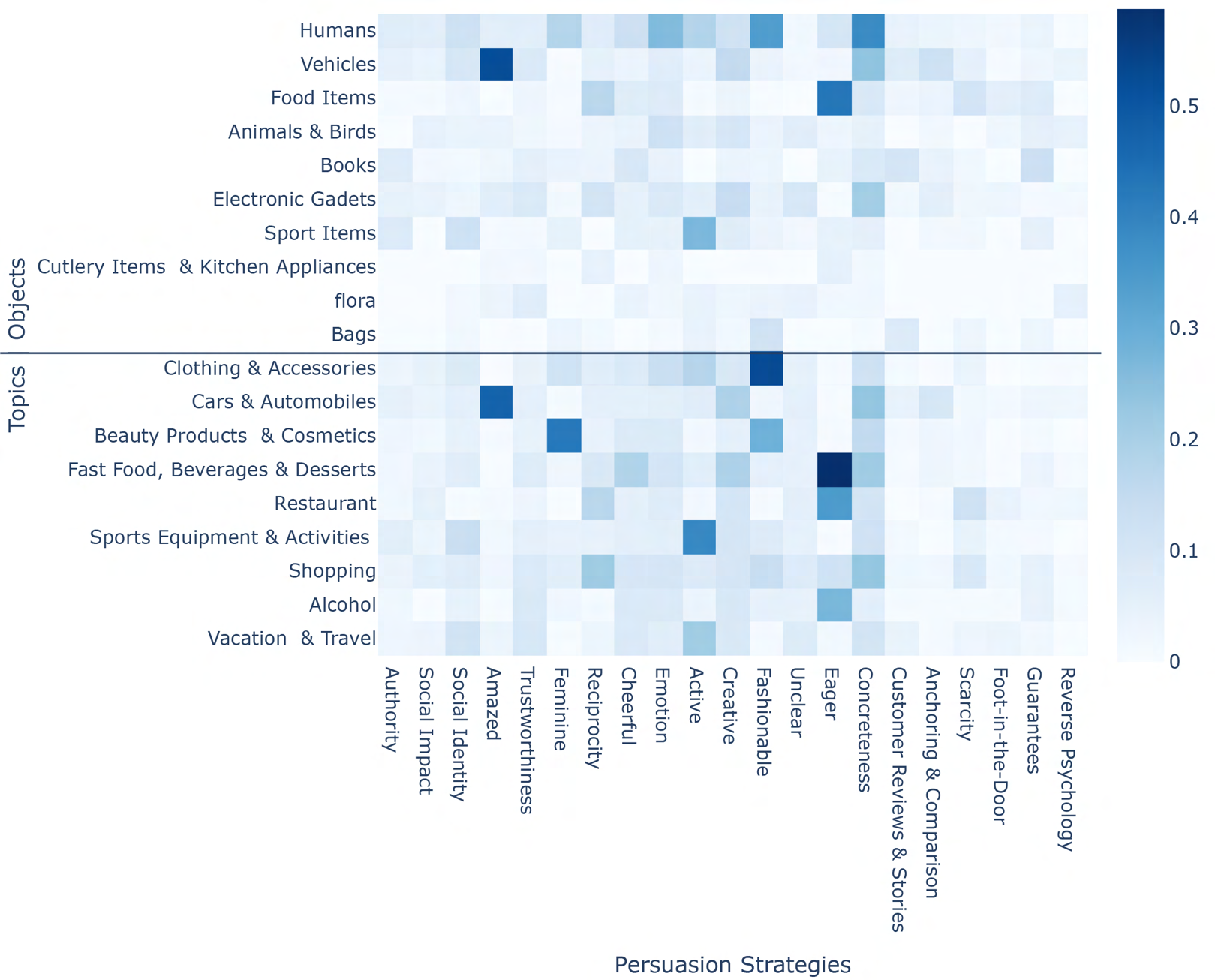
\includegraphics[scale=0.55]{images/objects_topics.pdf}
        \caption{Dice correlation between topics and strategies. Topics are taken from the Pitts Ad dataset and further similar topics are combined to get these values.}
        \label{fig:correlation-between-topics-and-strategies}
        % \vspace*{-3mm}
    \end{figure}

Next, we calculate the correlation between image topics and objects present with persuasion strategies. We see that the emotion:feminine and emotion:fashionable strategies are most often associated with beauty products and cosmetics (corr=0.4256, 0.2891). This is understandable since most beauty products are aimed at women. We see that the fast-food and restaurant industries often use eagerness as their messaging strategy (corr = 0.5877,0.3470). We find that the presence of humans in ads is correlated with the concreteness strategy (see Fig~\ref{fig:humans_concreteness-ads} for a few examples) (corr=0.3831). On the other hand, vehicle ads use emotion:amazed and concreteness (corr=0.5211,0.2412) (see Fig:\ref{fig:correlation-between-topics-and-strategies} for detailed correlations). 

Similar to a low correlation in co-occurring strategies, we find that product segments and their strategies are not highly correlated. This is because marketers use different strategies to market their products even within a product segment. Fig.~\ref{fig:footwear-strategies} shows an example in which the footwear industry (which is a subsegment of the apparel industry) uses different strategies to market its products. Further, for a batch of $250$ images, we also label segmented image regions corresponding to the strategies present in the image. These segment masks were also double-annotated. Fig.~\ref{fig:segmented image} presents an example of masks depicting parts of the image masked with different persuasion strategies in a drink advertisement.





\subsection{Persuasion Strategy Dataset For Video Advertisements}
For this task, we collected 2203 video advertisements from popular brands publicly available on the web. We use the following 12 strategies as our target persuasion strategy set: \textit{Social Identity, Concreteness, Anchoring and Comparison, Overcoming Reactance, Reciprocity, Foot-in-the-Door, Authority, Social Impact, Anthropomorphism, Scarcity, Social Proof,} and \textit{Unclear}. We use non-experts human annotators to label this dataset (as compared to expert humans for the image ads dataset). In order to make the class labels easier to understand for non-expert human annotators, we make a list of 15 yes/no type-questions containing questions like ``\textit{Was there any expert (person or company) (not celebrity) encouraging to use the product/brand? Was the company showcasing any awards (e.g., industrial or government)? Did the video show any customer reviews or testimonials?}'' (complete list in Table~\ref{table:persuasion strategy questions}). 

Each human annotator watches 15 videos such that each video gets viewed by at least two annotators and answers these questions for each video. Based on all the responses for a video, we assign labels to that video. We remove videos with an inter-annotator score of less than 60\%. After removing those, we get a dataset with 1002 videos, with an average length of 33 secs and a distribution as shown in Fig.~\ref{fig:persuasion-strategy-dataset-distribution}. This dataset is then used for the persuasion strategy identification task. 


\begin{figure}[!h]
    \centering
    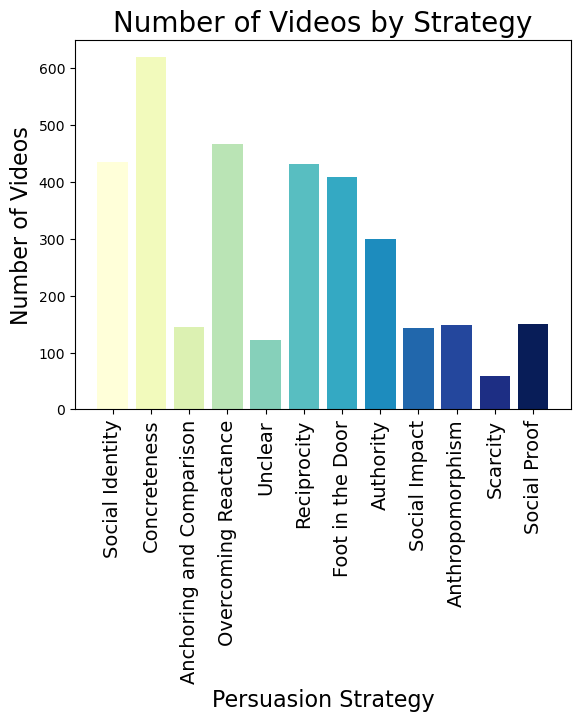
\includegraphics[width=0.5\textwidth]{images/video_strategies.png}
    \caption{Distribution of persuasion strategies in our video persuasion strategy dataset}
    \label{fig:persuasion-strategy-dataset-distribution}
\end{figure}


\begin{table*}[!hp]
  \centering
  \begin{tabular}{|p{3.5cm}|p{2.3cm}|p{3.5cm}|p{2.3cm}|}
    \hline
    \textbf{Question} & \textbf{Strategy} & \textbf{Question} & \textbf{Strategy} \\
    \hline
    Was there any expert (person or company) (not celebrity) encouraging to use the product/brand? & Authority & Did the video show any normal customers (non-expert, non-celebrity) using the product? & Social Identity \\
    \hline
    Did the video showcase any awards or long usage history of the product/brand? & Authority & Did the video show any customer reviews or testimonials? & Social Proof \\
    \hline
    Was the product/brand comparing itself with other competitors or existing solutions? & Anchoring and Comparison & Were any number/statistics mentioned? & Concreteness \\
    \hline
    Did the video talk about any specific features or provide information about the product/brand? & Concreteness & Were there any mention of any offers on the brand/product? & Reciprocity \\
    \hline
    Were the offers limited or available for a short period of time? & Scarcity & Was the product/brand told to be free or available on a discount? & Foot in the Door, Reciprocity \\
    \hline
    Was the brand/product described as simple, easy to use, or can start using with minimal resistance? & Overcoming Reactance, Foot in the Door & Was the brand/product talking about bigger societal impact? & Social Impact \\
    \hline
    Did the brand provide any guarantees that might help reduce the risk of people trying out the product? & Overcoming Reactance & Did the video provide any resources, tips, guides, or tools related to the product? & Reciprocity \\
    \hline
    Is the brand or product portrayed as human-like? & \makecell{Anthropo-\\morphism} & & \\
    \hline
  \end{tabular}
  \caption{The questions we asked to the non-expert annotators to help them identify persuasion strategy contained in the video advertisement. \label{table:persuasion strategy questions}}
\end{table*}





% \vspace{-2mm}
\section{Modeling: Persuasion Strategy Prediction}
\label{sec:Persuasion Strategy Prediction Model}


\begin{figure}[!h]
    \centering
    \begin{subfigure}[b]{0.49\textwidth}
         \centering
         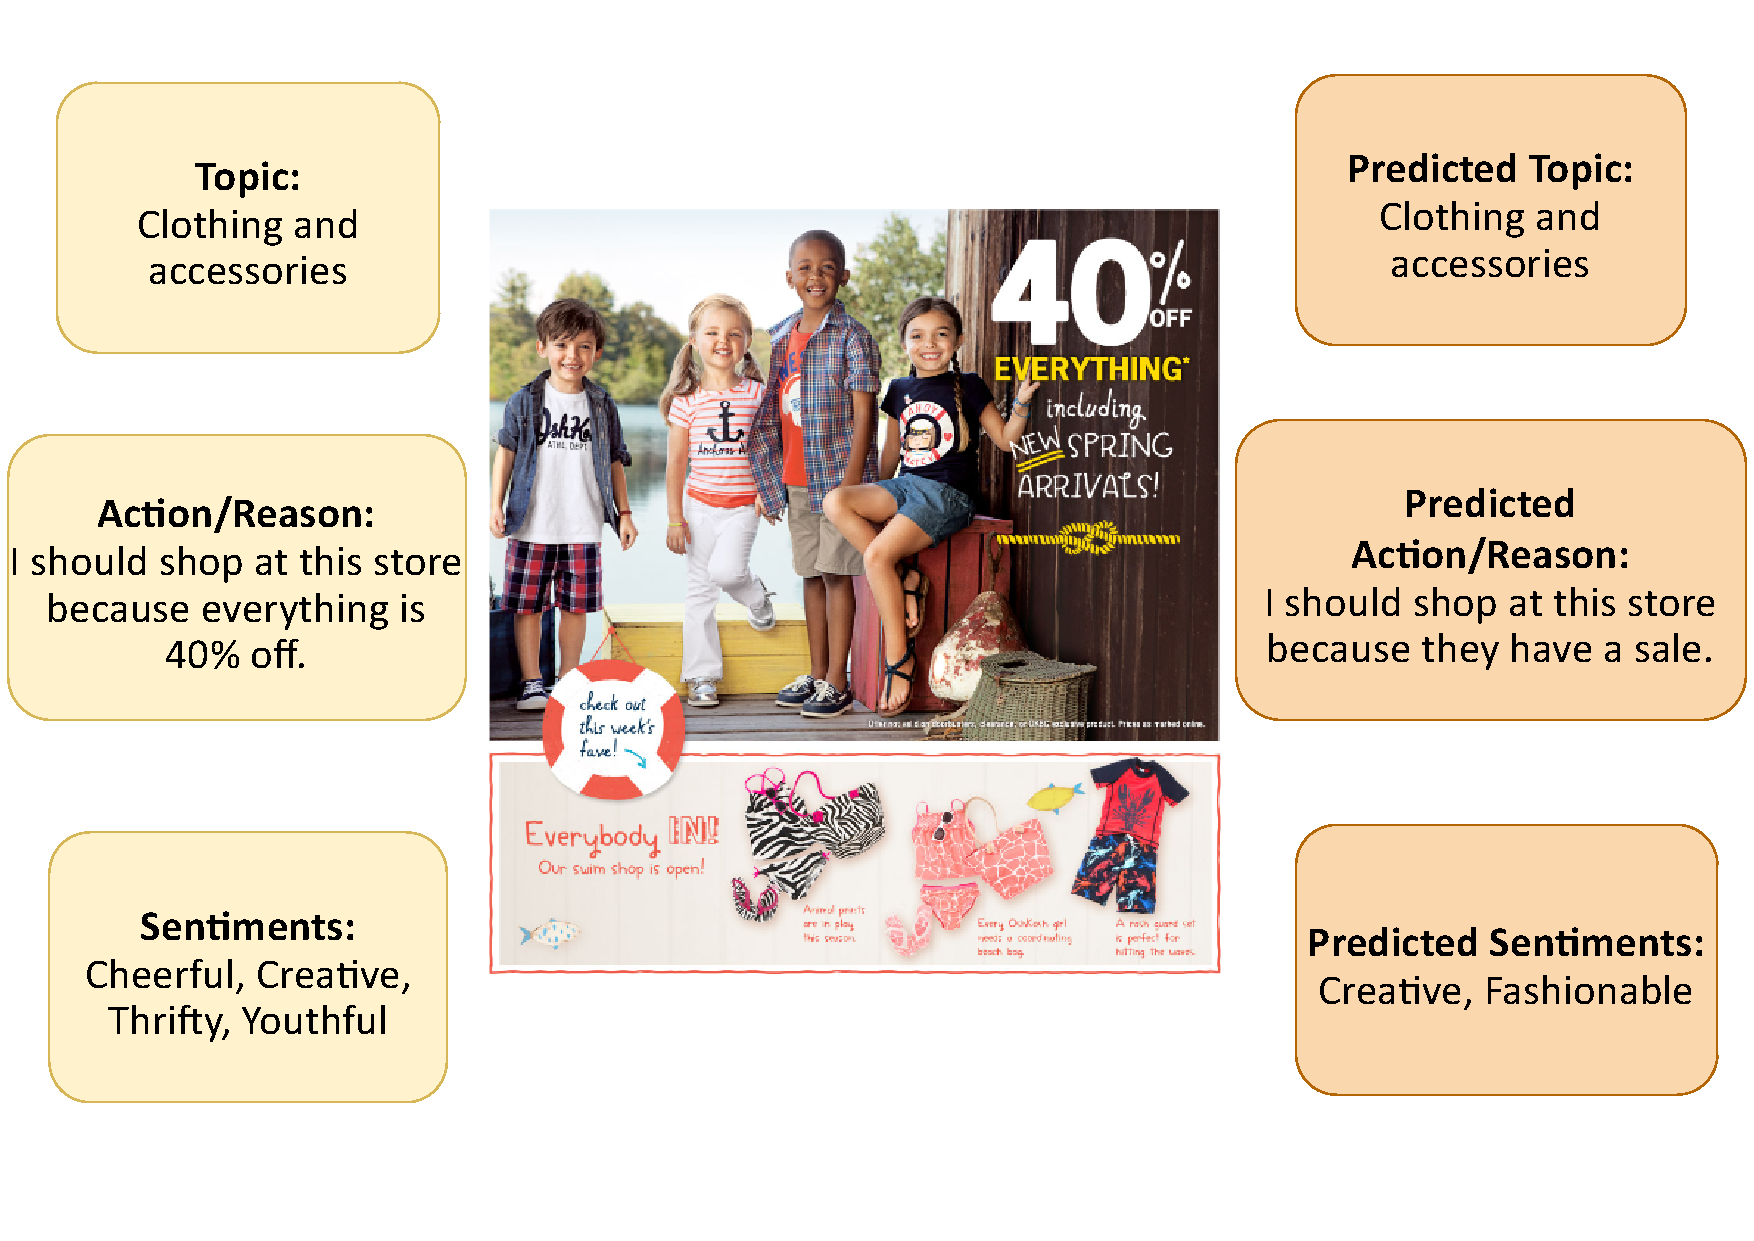
\includegraphics[width=\textwidth,scale=0.68]{images/preds_sup_1.pdf}
         \caption{}
         \label{fig:preds-sup-1}
        %  \vspace{-3pt}
     \end{subfigure}
     \begin{subfigure}[b]{0.49\textwidth}
         \centering
         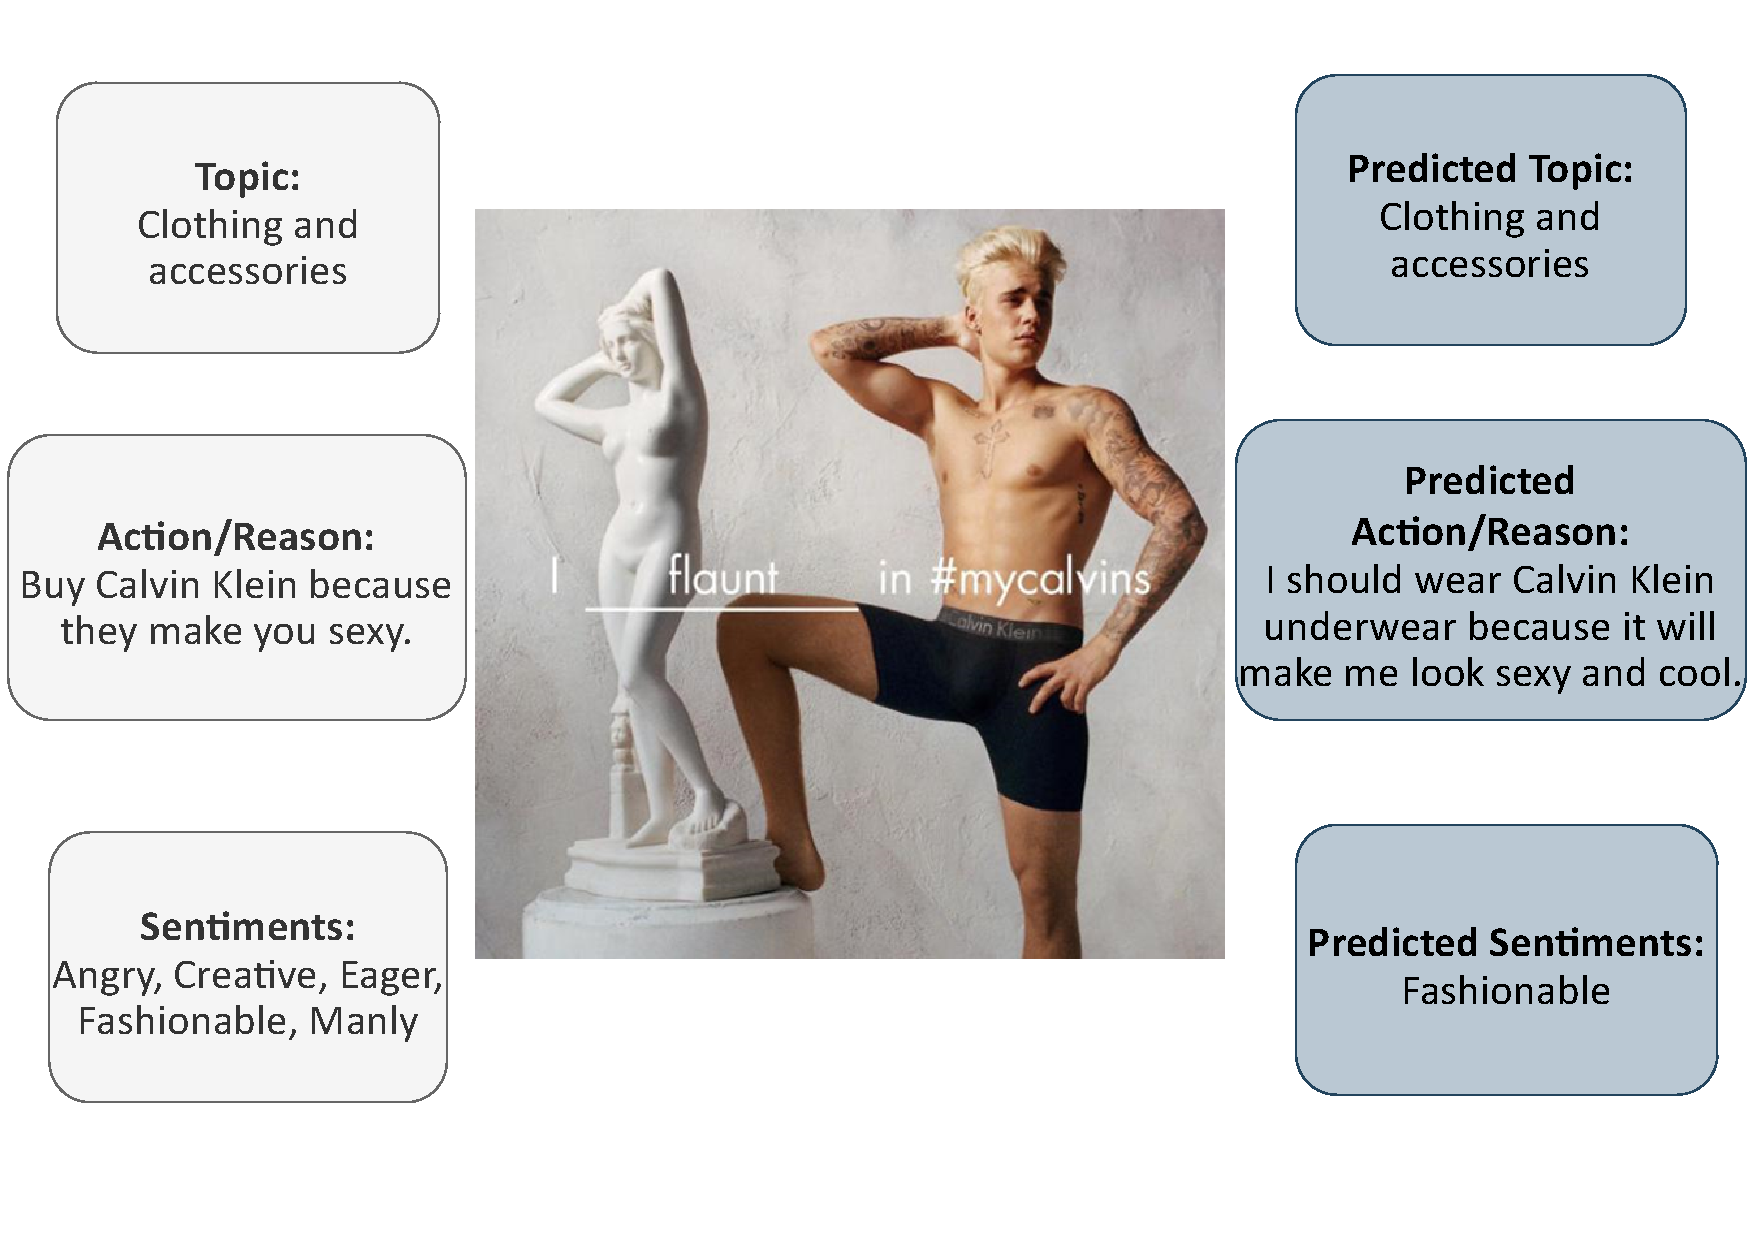
\includegraphics[width=\textwidth,scale=0.68]{images/preds_sup_2.pdf}
         \caption{}
         \label{fig:preds-sup-2}
        %  \vspace{-3pt}
     \end{subfigure}
    %  \begin{subfigure}[b]{0.49\textwidth}
    %      \centering
    %      \includegraphics[width=0.8\textwidth,scale=0.68]{LaTeX/images/preds_sup_5.pdf}
    %      \caption{}
    %      \label{fig:preds-sup-5}
    %      \vspace{-10pt}
    %  \end{subfigure}
     \begin{subfigure}[b]{0.49\textwidth}
         \centering
         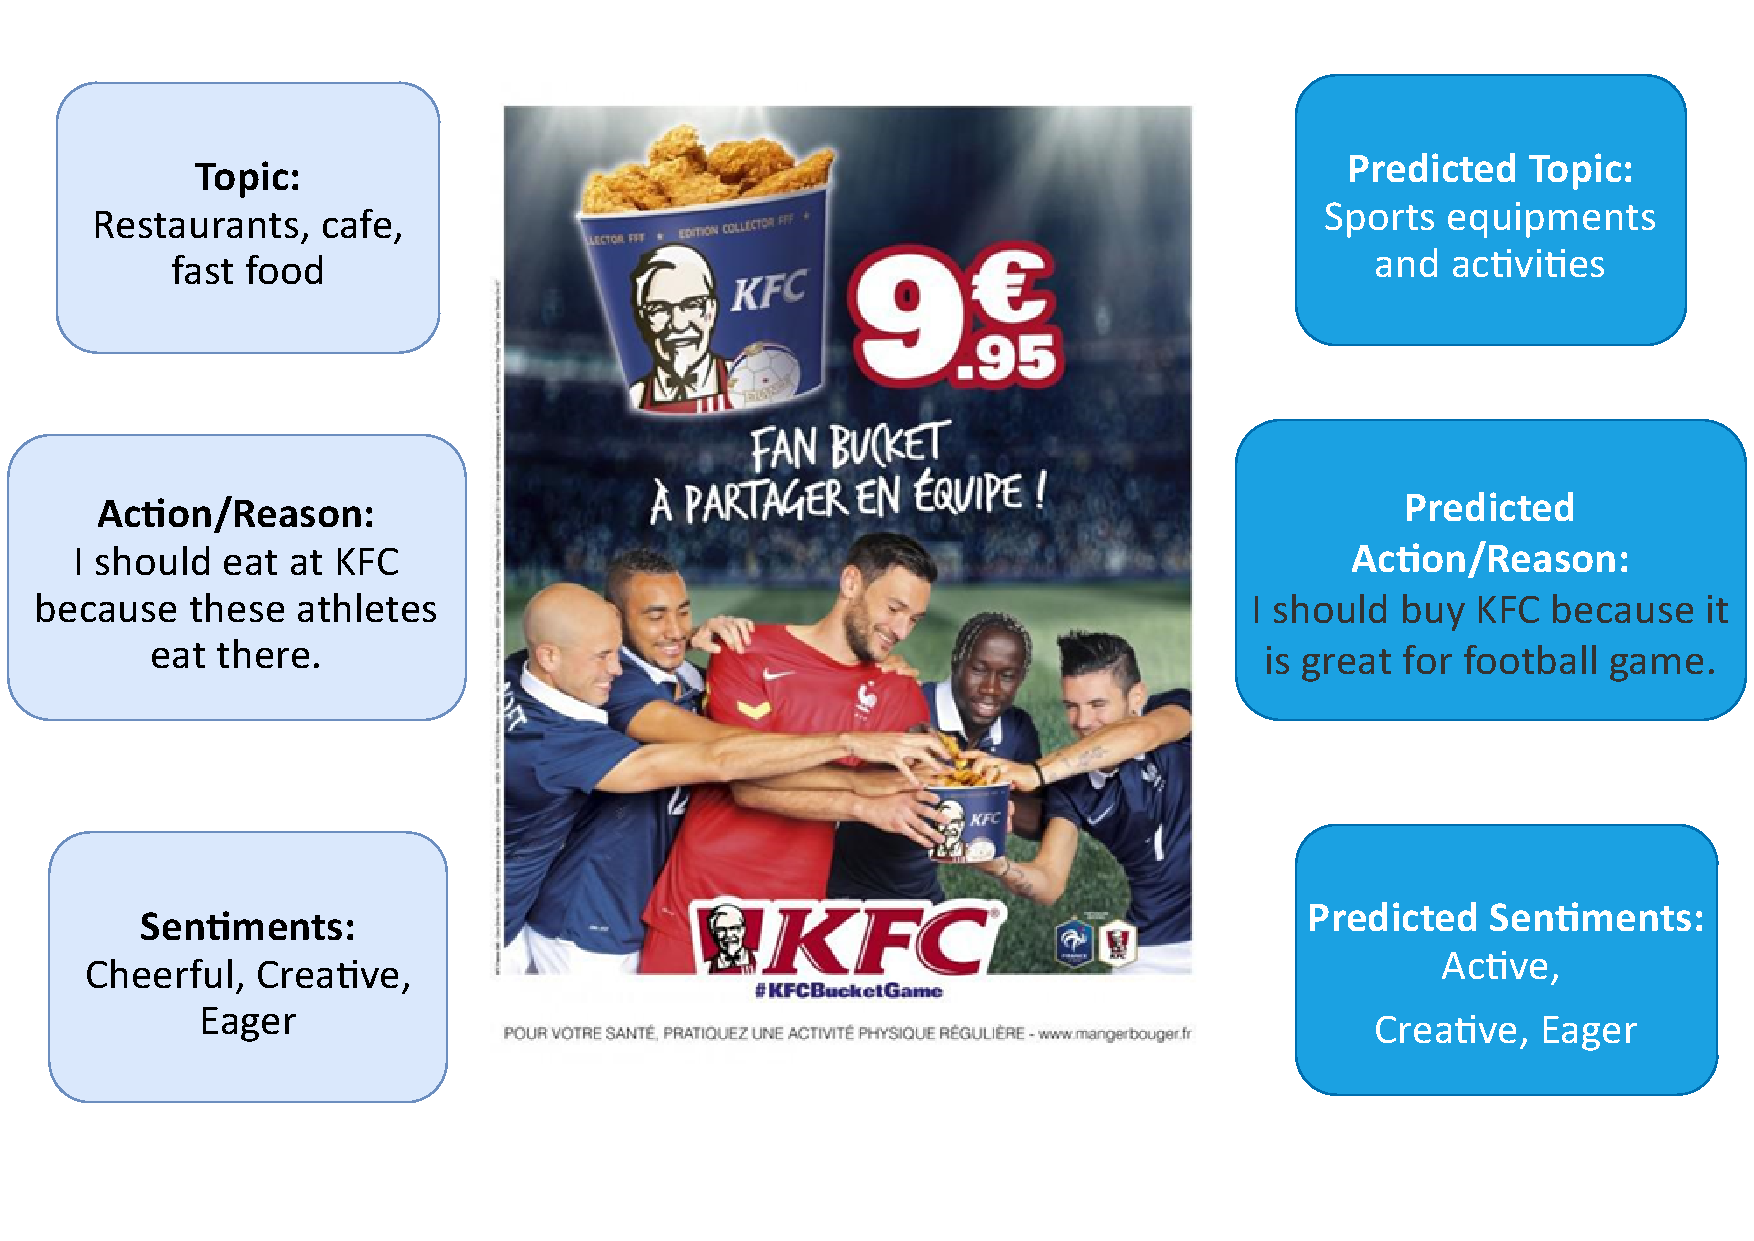
\includegraphics[width=\textwidth,scale=0.68]{images/preds_sup_8.pdf}
         \caption{}
         \label{fig:preds-sup-8}
            % \vspace{-10pt}
     \end{subfigure}
    \caption{Some samples from the Pitts Ads dataset along with the ground truth and predicted action-reason statement, topic and sentiments.}
    \label{fig:preds-sup}
\end{figure}


\subsection{Modelling Persuasion Strategy For Image Advertisements}
The proposed Ads dataset $\mathcal{D}$ annotated with the persuasion strategies comprises of samples where each sample advertisement $a_i$ is annotated with a set of annotation strategies $S_i$ such that $1\le|{S_i}|\le3$. The unique set of the proposed persuasion strategies $\mathcal{P}$ is defined in Table~\ref{tab:persuasive-strategies-list}. Given $a_i$, the task of the modeling is to predict the persuasion strategies present in the input ad. As we observe from Fig.~\ref{fig:persuasion-strategies-headline-image}, advertisements use various rhetoric devices to form their messaging strategy. The strategies thus are in the form of multi-modalities, including images, text and symbolism. To jointly model the modalities, we design an attention fusion multi-modal framework, which fuses multimodal features extracted from the ad, {\it e.g.}, the ad image, text present in the ad extracted through the OCR (Optical Character Recognition), regions of interest (ROIs) extracted using an object detector, and embeddings of captions obtained through an image captioning model (see Fig.~\ref{fig:arch_diag}). The information obtained through these modalities are firstly embedded independently through their modality specific encoders followed by a transformer-based cross-attention module to fuse the extracted features from different modalities. The fused embeddings from the attention module are then used as input for a classifier that predicts a probability score for each strategy $p \in \mathcal{P}$. The overall architecture of the proposed model is illustrated in Fig.\ref{fig:arch_diag}. In the following, we describe each step in the prediction pipeline in detail.






\iffalse
{\small%
\begin{table}[]
\small
      \resizebox{0.8\columnwidth}{!}{%
      \begin{tabular}{ll}
            \toprule
             \textbf{Strategies} & \textbf{Corr}\\ \midrule
              Eager-Concreteness & 0.268 \\\midrule
             Scarcity-Reciprocity & 0.253 \\\midrule
             Eager-Cheerful  & 0.187 \\\midrule
             Amazed-Concreteness & 0.174 \\\midrule
             Eager-Reciprocity & 0.165 \\\bottomrule
        \end{tabular}}
        \caption{\looseness=-1 Top-5 Dice Correlated Persuasion Strategies. In general, we observe that persuasion strategies are not heavily correlated with each other. This means that the marketers are using unique combinations of messaging strategies to market their products.}
        \label{tab:top-5-correlated strategies}
    \end{table}}
\fi

\begin{figure*}[h]
% \vspace*{-11mm}
        \centering
        % \includegraphics[scale=0.28]{images/Model_Architecture.pdf}
        % \includegraphics[scale=0.185]{images/Persuasion Arch Diag - Copy of Model_Architecture-Page-2.drawio.png}
        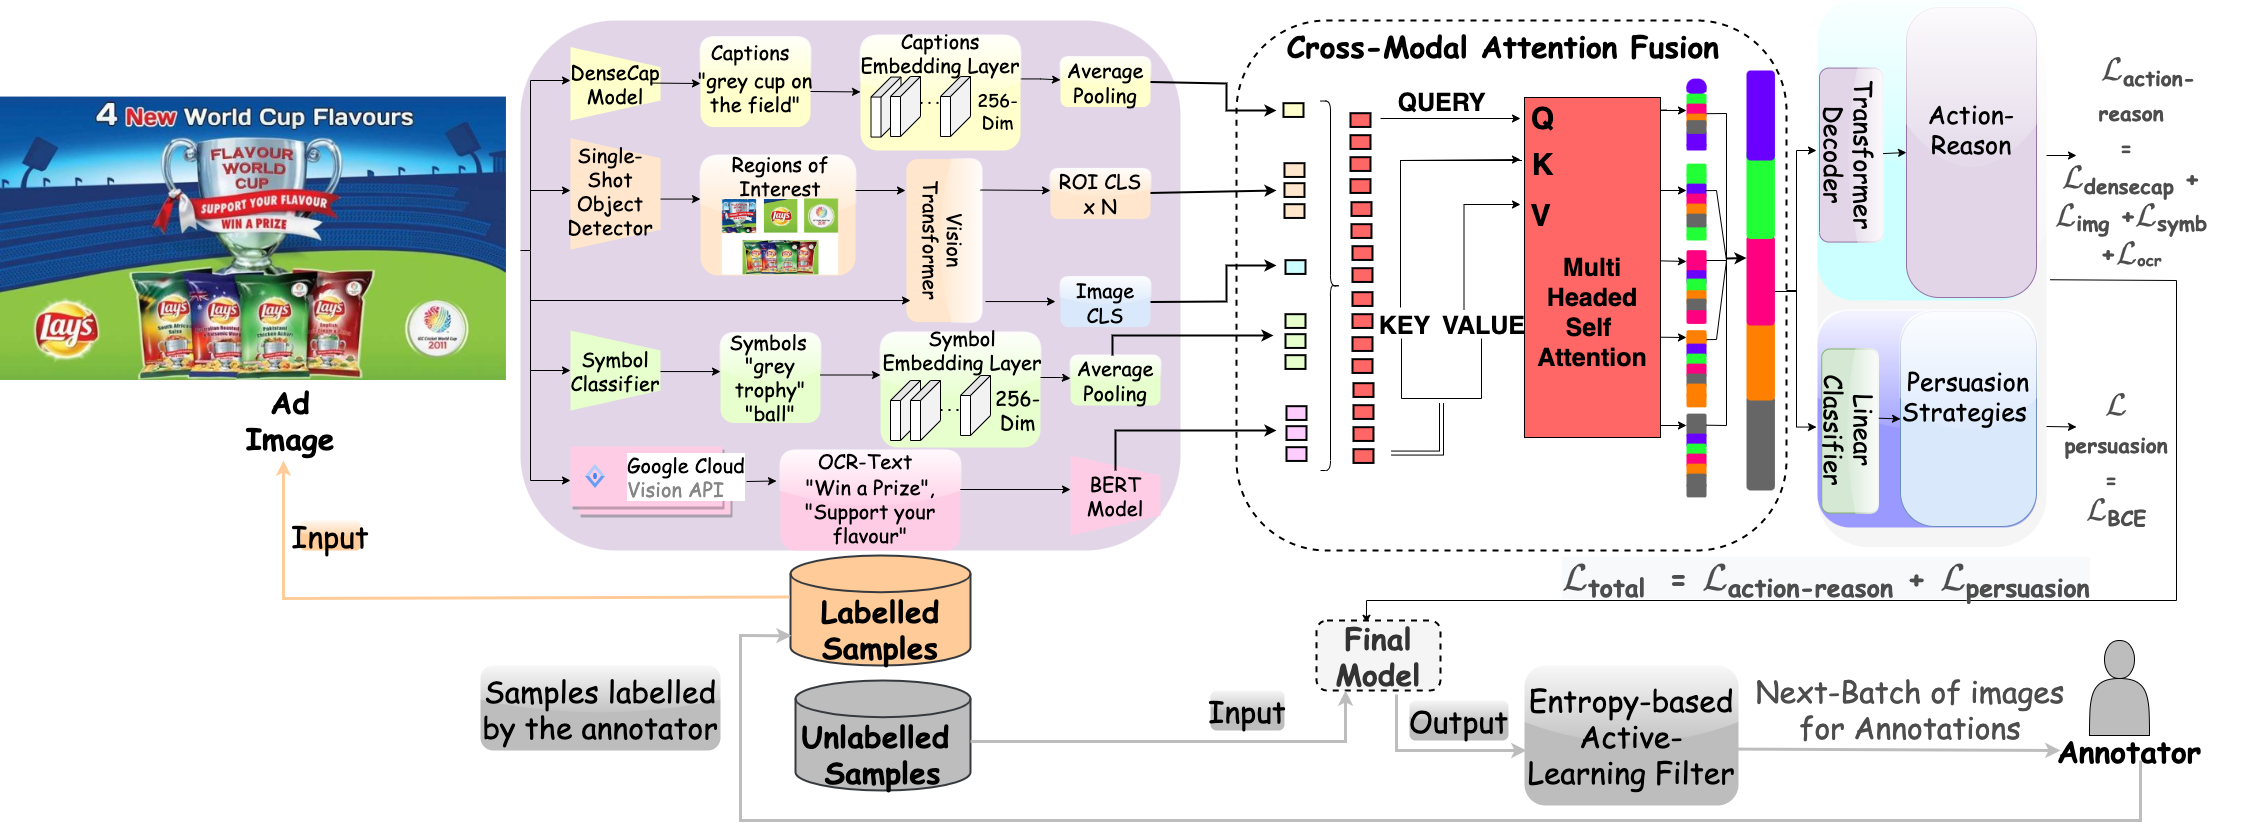
\includegraphics[width=\textwidth]{images/Persuasion-Arch-Diag-Copy-of-Model_Architecture-Page-2.drawio.png}
        % \vspace*{-2mm}
        \caption{\small Architecture of the Persuasion Strategy Prediction model. To capture the different rhetoric devices, we extract features for the image, text, and symbolism modalities and then apply cross-modal attention fusion to leverage the interdependence of the different devices. Further, the model trains over two tasks: persuasion strategies and the reasoning task of action-reason prediction.}
        % \label{fig:persuasion-strategies-headline-image}
% \vspace*{-4mm}
\label{fig:arch_diag}
\end{figure*}




\subsubsection{Feature Extractors} 

In order to capture different rhetoric devices, we extract features from the image, text, and symbolism modalities.

\textbf{Image Feature:} We use the Vision Transformer \cite{dosovitskiy2020image} (ViT) model for extracting image features from the entire input image. The model resizes the input image to size $224 \times 224$ and divides it into patches of size $16 \times 16$. The model used has been pre-trained on the ImageNet 21k dataset. We only use the first output embedding, which is the CLS token embedding, a $768$ dimension tensor, as we only need a representation of the entire image. Then, a fully connected layer is used to reduce the size of the embedding, resulting in a tensor of dimension $256$.




\textbf{Regions of Interest (RoIs) from Detected Objects and Captions:} %The major difference between creative and natural images is the presence of composing elements \cite{zitnick2013bringing,zitnick2014adopting}. 
Ad images contain elements that the creator deliberately chooses to create \textit{intentional impact} and deliver some \textit{message} in addition to the ones that occur \textit{naturally} in the environment. Therefore, it is important to identify the composing elements of an advertisement to understand the creator's intention and the ad's message to the viewer. We detect and extract objects as regions of interest (RoIs) from the advertisement images. We get the RoIs by training the single-shot object detector model \cite{liu2016ssd} on the COCO dataset \cite{lin2014microsoft}. We compare it with the recent YOLOv5 model \cite{redmon2016you}. We also extract caption embeddings to detect the most important activity from the image using a caption generation mode. We compare DenseCap \cite{yang2017dense} and the more recent BLIP \cite{li2022blip} for caption generation.





\textbf{OCR Text:} The text present in an ad presents valuable information about the brand, such as product details, statistics, reasons to buy the product, and creative information in the form of slogans and jingles that the company wants its customers to remember and thus making it helpful in decoding various persuasion strategies. Therefore, we extract the text from the ads and use it as a feature in our model. We use the Google Cloud Vision API for this purpose. All the extracted text is concatenated, and the size is restricted to $100$ words. We pass the text through a BERT model and concatenate the embeddings for those 100 words. Similar to image embeddings, an FC layer is used to convert embeddings to 256 dimensions. The final embedding of the OCR is a tensor of dimension $100 \times 256$. 


\textbf{Symbolism:} While the names of the detected objects convey the names or literal meaning of the objects, creative images often also use objects for their symbolic and figurative meanings. For example, an upward-going arrow represents growth or the north direction or movement towards the upward direction depending on the context; similarly, a person with both hands pointing upward could mean danger (\textit{e.g.}, when a gun is pointed) or joy (\textit{e.g.}, during dancing). In Fig.~\ref{fig:persuasion-strategies-headline-image}, in the creative Microsoft ad, a symbol of a balloon is created by grouping multiple mice together. Therefore, we generate symbol embeddings to capture the symbolism behind the most prominent visual objects present in an ad. We use the symbol classifier by Hussain \textit{et al.} \cite{hussain2017automatic} on ad images to find the distribution of the symbolic elements present and then convert this to a $256$ dimension tensor. %Finally we get a $2 \times 256$ dimension tensor.


\subsubsection{Cross-Modal Attention} 
To capture the inter-dependency of multiple modalities for richer embeddings, we apply a cross-modal attention (CMA) layer~\cite{frank2021vision} to the features extracted in the previous steps. Cross-modal attention is a fusion mechanism where the attention masks from one modality (\textit{e.g.} text) are used to highlight the extracted features in another modality (\textit{e.g.} symbolism). It helps to link and extract common features in two or more modalities since common elements exist across multiple modalities, which complete and reinforce the message conveyed in the ad. For example, the pictures of the silver cup, stadium, and ball, words like ``Australian'', ``Pakistani'', and ``World Cup'' present in the chips ad shown in Fig.~\ref{fig:arch_diag} link the idea of buying \textit{Lays} with supporting one's country's team in the World Cup. Cross attention can also generate effective representations in the case of missing or noisy data or annotations in one or more modalities \cite{frank2021vision}. This is helpful in our case since marketing data often uses implicit associations and relations to convey meaning. 

The input to the cross-modal attention layer is constructed by concatenating the image, RoI, OCR, caption, and symbol embeddings. This results in a $114 \times 256$ dimension input to our attention layer. The cross-modal attention consists of two layers of transformer encoders with a hidden dimension size of $256$. %The rest of the hyper-parameters are similar to the ones given in the original paper \cite{vaswani2017attention}. 
The output of the attention layer gives us the final combined embedding of our input ad. 
Given image embeddings $E_i$, RoI embeddings $E_r$, OCR embeddings $E_o$, caption embeddings $E_c$ and symbol embeddings $E_s$, the output of the cross-attention layer $E_{att}$ is formulated as:
\begin{align}
        \text{Enc}(X) &= \text{CMA}(\left[E_i(X),E_r(X), E_o(X),E_c(X),E_s(X)\right])\,, \nonumber
\end{align}
where $[\ldots,\ldots]$ is the concatenation operation. For the advertisement in Fig.~\ref{fig:arch_diag}, we observed that the caption ``grey cup on the field'' attends to OCR text (containing words like ``win'') and ViT features of the RoI (of ``cup'' and ``field'').

%We propose solving the following tasks for understanding advertisements: action-reason generation, topic classification, and sentiment detection. For solving these, we consider a multi-task learning framework where each task has a task-specific network built upon a common, shared multi-modal encoder. We learn the shared parameters $\thetav_s$ and a set of task-specific parameters $\{\thetav_i\}^{T}_{i=1}$ for $T$ tasks. Our goal is to learn parameters $\thetav_s \cup \{\thetav_i\}^{T}_{i=1}$ that minimize loss across all tasks. Details on different tasks and loss designs are introduced next. In our specific setting, we have $T=3$.


\subsubsection{Persuasion Strategy Predictor} 
This module is a persuasion strategy predictor, which processes the set of feature embedding \text{Enc}(X) obtained through cross-modality fusion. Specifically, \text{Enc}(X) is passed through a self-attention layer as:
\begin{align}
o_{1} = softmax(\text{Enc}(X) \otimes W_{self-attn})^\intercal \otimes \text{Enc}(X)
\end{align}
where \text{Enc}(X) is of the dimension $114\times256$,  $W_{self-attn} \in \mathcal{R}^{256 \times 1}$, $\otimes$ denote tensor multiplication and $o_1$ denotes the output of self attention layer, which is further processed through a linear layer to obtain $o_{|\mathcal{P}|}$ to represent the logits for each persuasion strategy. We apply sigmoid over each output logit such that the $i^{th}$ index of the vector after applying sigmoid denotes $p_i$ - the probability with which $i^{th}$ persuasion strategy is present in the ad image. Our choice of using sigmoid over softmax is motivated by the fact that multiple persuasion strategies can be present simultaneously in an ad image. Consequently, the entire model is trained in an end-to-end manner using binary cross-entropy loss $\mathcal{L}_{s}$ over logit for each strategy:
\begin{align}
        \mathcal{L}_{s} = \left[-y_i \log(p_i) - (1-y_i) \log(1 - p_i) \right]
\end{align}
where, $y_i$ is 1 if $i^{th}$ persuasion strategy is present in the ad and 0 otherwise. It can be observed in Table~\ref{tab:modalities} that our model achieves an accuracy of $59.2\%$, where a correct match is considered if the strategy predicted by the model is present in the set of annotated strategies for a given ad. Further, we perform several ablations where we exclude each modality while retaining all the other modalities. We note that for each modality, excluding the modality results in a noticeable decrease in accuracy, with significant decreases observed when excluding DenseCap ($\sim3.6\%$) and OCR ($\sim4.4\%$). Further, we observe that using DenseCap for obtaining caption embeddings, and SSD for object detection works better than BLIP and YOLOv5, respectively (see Table~\ref{tab:varying_cap_obj}). We also explore using focal loss~\cite{lin2017focal} in place of cross-entropy loss to handle class imbalance but observed that it led to degradation instead of improvements (top-1 acc.\footnote{\textit{Top-1 Accuracy}: It is defined as the fraction of images, where the highest predicted strategy is present in the ground-truth strategies. \textit{Top-3 Accuracy} : It is defined as the fraction of images, where any of the top-3 highest predicted strategies is present in the ground-truth strategies.} of $56.4\%$ \textit{vs} $59.2\%$ using cross-entropy). We also train the model of Hussain \textit{et al.} \cite{hussain2017automatic} for strategy prediction through a similar configuration as ours (along with action-reason generation using an LSTM branch). We find that their top-1 and top-3 accuracy is 52.4\% (vs. 59.2\% ours) and 75.7\% (vs. 84.8\% ours), which is lesser compared to our model.

\begin{table}[t]
% \vspace{-8mm}
    \small
        \centering
        %\begin{adjustbox}{width=\columnwidth,center}
        \resizebox{0.8\columnwidth}{!}{%
       \begin{tabular}{lll}%[tab1,tabularx={XYYYYY}]
             \textbf{\thead{Models}} & \textbf{\thead{Top-1  Acc.}} & \textbf{\thead{Top-3 Acc.}}\\ \midrule
             Our Model & \textbf{59.2} & \textbf{84.8} \\ \midrule
             w/o DenseCap & 55.6 & 80.8 \\ \midrule
             w/o Symbol   & 58.8 & 81.6 \\ \midrule
           w/o DenseCap \& Symbol & 55.2 & 80.8 \\ \midrule
            w/o OCR & 54.8 & 82 \\ \midrule
            w/o Symbol,\\OCR \& DenseCap & 58 & 78.8 \\ \midrule
                %  With Topic & 43.2 & 67.2 \\ \bottomrule
            w/o Action-Reason Task & 56.4 & 80.4\\ \midrule
            Random Guess & 6.25 &  18.75\\\bottomrule
        \end{tabular}}
        \caption{\small Effect of different Modalities and Tasks on the accuracy and performance of the strategy prediction task.}
        % \vspace{-3mm}
        %\end{adjustbox}
        \label{tab:modalities}
    \end{table}

\subsubsection{Multi Task Learning}
One of the key opportunities for our persuasion strategies data labeling and modeling task was the presence of additional labels already given in the base Pitts Ads dataset. In that, authors had given labels about the reasoning task. For the reasoning task, the annotators were asked to provide answers in the form ``I should [Action] because [Reason]." for each ad. In other words, they asked the annotators to describe \textit{what the viewer should do and why}, according to
the ad. Similar to the reasoning task, persuasion strategies provide various cognitive, behavioral, and affective reasons to try to elicit the motivation of the ad viewers towards their products or services. Therefore, we hypothesize that these natural language descriptions of \textit{why the viewers should follow} the ad will be informative in inferring the ad's persuasion strategy.

We formulate obtaining action-reason statement as a sequence generation task where the model learns to generate a sentence $Y^g=(y^g_1, \ldots, y^g_T)$ of length $T$ conditioned on advertisement $X$ by generating the sequence of tokens present in the action-reason statement. To achieve this, we use a transformer decoder module that attends on the features $\text{Enc}(X)$ as shown in Fig.~\ref{fig:arch_diag}. The annotated action-reason statement is used to train the transformer decoder as an auxiliary task to strategy prediction through the standard teacher forcing technique used in Seq2Seq framework. Please refer to the Supplementary for more architectural details about the action-reason generation branch. As shown in Table~\ref{tab:modalities}, generating action-reason as an auxiliary task improves the strategy prediction accuracy by $2.8\%$. We evaluate the performance on action-reason generation on following metrics: BLEU-1, BLEU-2, BLEU-3, BLEU-4, METEOR, ROUGE, CIDER, SPICE and observed a score of 53.6, 42.0, 33.1, 25.7, 26.3, 48.4, 42.8, 8.9 respectively.


% task Ti dataset Di consisting  of ni training  samples,  i.e.,Di={xij,yij}nij=1,  where xij∈Rdi is the jth training instance in Ti and yi ji s its label. We denote byXithe  training  data  matrix  forTi,  i.e.,Xi= (xi1,...,xini)

% \vspace{-1mm}

\begin{table}[!t]
        \small
        \centering
        % \vspace{-8mm}

        %\begin{adjustbox}{width=\columnwidth,center}
        \resizebox{0.8\columnwidth}{!}{%
       \begin{tabular}{llllll}%[tab1,tabularx={XYYYYY}]
                \textbf{\thead{Model Used}} & \textbf{\thead{Top-1 \\Accuracy}} & \textbf{\thead{Top-3 \\Accuracy}} &  \textbf{Recall} \\ \midrule
                 Model with \\DenseCap \& SSD & 59.2 & 84.8 & 74.59\\ \midrule
                 Model with \\BLIP \& YOLOv5 & 58.4 &  83.8 & 71.58 \\ \midrule
        \end{tabular}}
        \caption{\small Comparison of caption and object detection models. We noticed that BLIP while being more recent and trained on a larger dataset, generates more informatory captions for background objects which DenseCap successfully ignores.}
        % \vspace{-3mm}
        %\end{adjustbox}
        \label{tab:varying_cap_obj}
    \end{table}
        \begin{figure}[h]
        \centering
        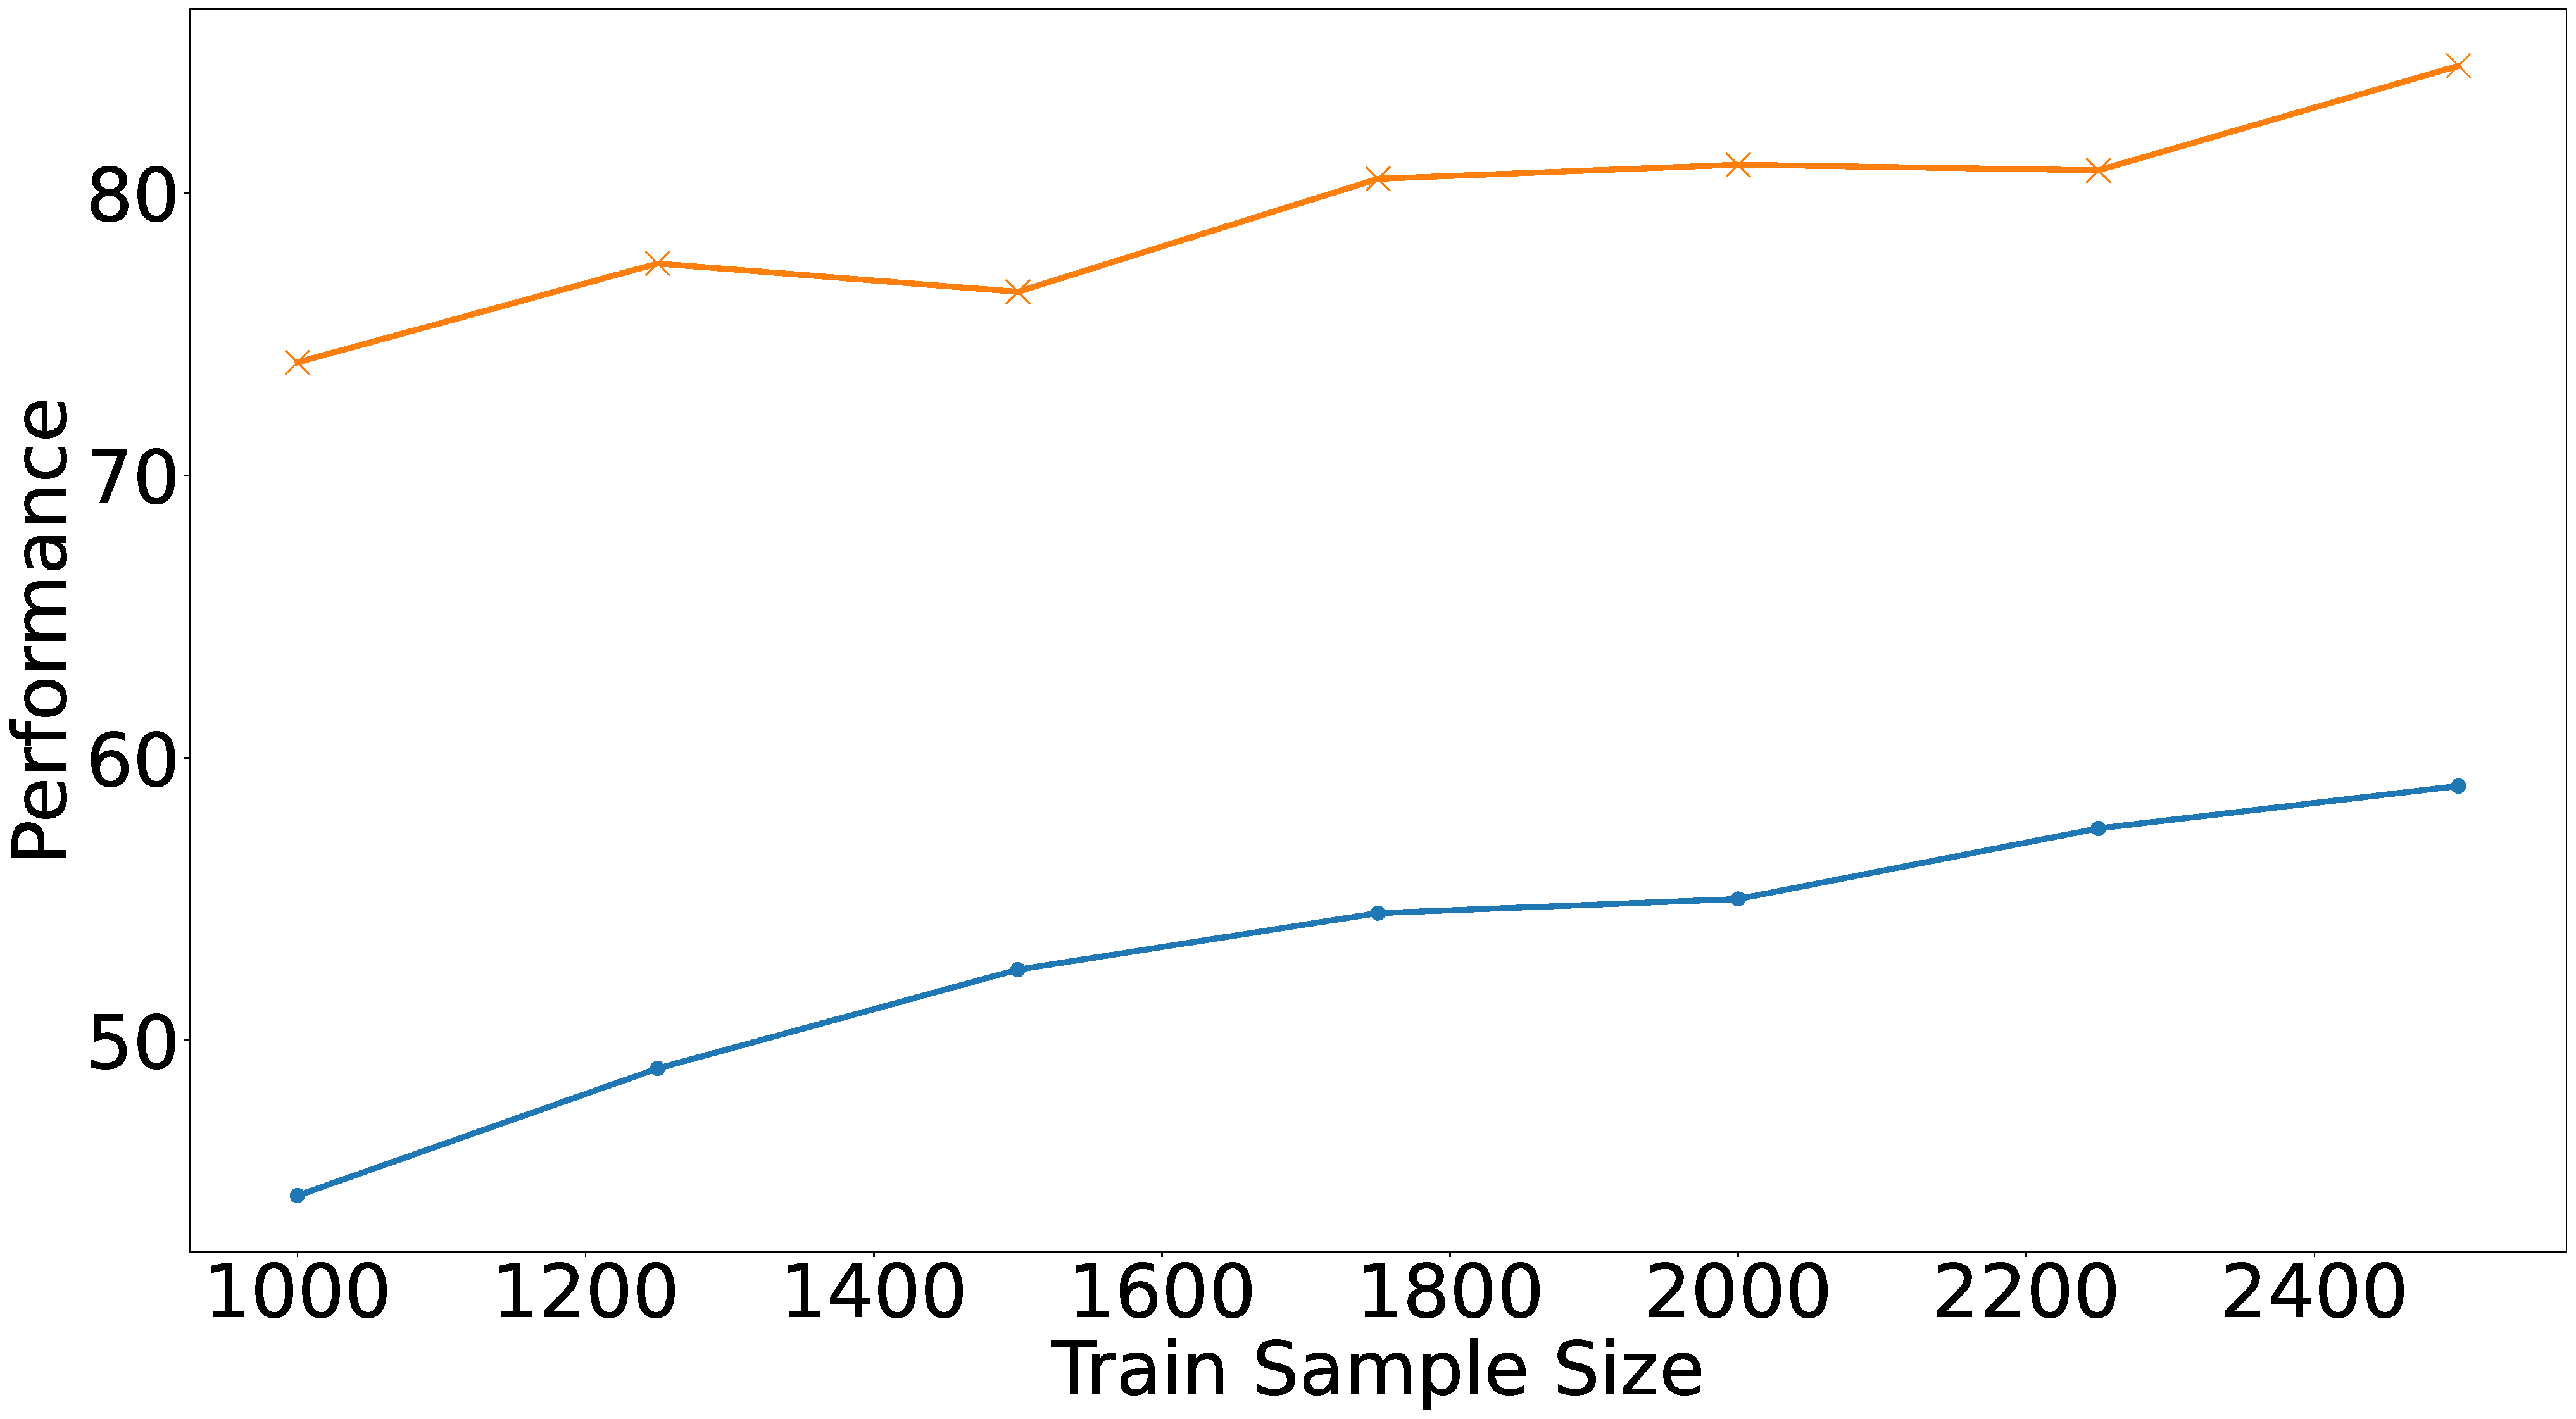
\includegraphics[scale=0.12]{images/active_learning.pdf}
        \caption{\small Incremental effect of introducing new data through active learning; Results for prediction of persuasion strategies on the test set}
        % \vspace{-4mm}
        \label{fig:AL_batch_test}
    \end{figure}


\begin{table}[]
    \small
        \centering
        %\begin{adjustbox}{width=\columnwidth,center}
        \resizebox{\textwidth}{!}{%
       \begin{tabular}{llllll}%[tab1,tabularx={XYYYYY}]
             & \textbf{\thead{\#ads with \\1 strategy}} & \textbf{\thead{\#ads with \\2 strategies}} & \textbf{\thead{\#ads with \\3 strategies}} & \textbf{\thead{Avg.\\strategies}} & \textbf{\thead{Std.\\Dev.}}\\ \midrule
             Train-Set & 1440 & 905 & 155 & 1.486 & 0.612 \\\midrule
             Val-Set & 132 & 98 & 20 & 1.552  & 0.639 \\\midrule
             Test-Set & 147 & 93 & 10 & 1.452 &0.574\\\midrule\midrule
             Total & 1719 & 1096 & 185 & 1.49 & 0.592 \\\bottomrule
        \end{tabular}}
        \caption{\small Distribution of test, train, validation, and the total dataset}
        \label{table:strategy-train-test-val-stats}
        % \vspace*{-3mm}
        %\end{adjustbox}
    \end{table}



\subsubsection{Active Learning}
We use an active learning method to ease the large-scale label dependence when constructing the dataset. As in every active learning setting, our goal is to develop a learner that selects samples from unlabeled sets to be annotated by an oracle. Similar to traditional active learners \cite{gilad2005query,lewis1994heterogeneous}, we use uncertainty sampling to perform the sample selection. In doing so, such function learns to score the unlabeled samples based on the expected performance gain they are likely to produce and used to update the current version of the localization model being trained. To evaluate each learner, we measure the performance improvements, assessed on a labeled test set at different training dataset sizes.


At every learning step $t$, a set of labeled samples $L_t$ is first used to train a model
$f_t$. Then, from an unlabeled pool $U_t=D-L_t$, an image instance $a$ is chosen by a selection function $g$. Afterwards, an oracle provides temporal ground-truth for the selected instance, and the labeled set $L_t$ is augmented with this new annotation. This process repeats until the desired performance is reached or the set $U_t$ is empty.

In our implementation, we instantiate the active learning selection function as the entropy of the probability distribution predicted by the model over the set of persuasion strategies for a given ad image instance $a$. Formally, $g = -\sum_{i=1}^{|\mathcal{P}|}p^{n}_{i}*\log(p^{n}_i)$, where $p^{n}_i$ denotes the normalized probability with which $i^{th}$ persuasion strategy is present in $a$ as per the model prediction. The normalized probability $p^{n}_{i}$ is estimated as $p_i/\sum_{j=1}^{|\mathcal{P}|}p_j$. Intuitively, ad samples with high entropy selection values indicate that the model trained on limited data has a higher degree of confusion while predicting the persuasion strategy since it is not decisively confident about predicting few strategies. Hence, we rank the unlabeled ad images in the decreasing order of difficulty according to the corresponding values of the entropy selection function and select the top-k ads in the subsequent batch for annotation followed by training. As shown in Fig.~\ref{fig:AL_batch_test}, we set k to be 250 and analyze the effect of incrementally introducing new samples selected through active learning. It can be seen that both top-1 and top-3 accuracy increases with the addition of new training data. We stop at the point when 2500 training samples are used since the model performs reasonably well with a top-1 and top-3 strategy prediction accuracy of 59.2\% and 84.8\% (see Fig.~\ref{fig:AL_batch_test}). 



%%%%%%%%%%%%%%%%%%%%%%%%%%%%%%%%%%%%%%%%%%%%%%%%%%%%%%%%%%%%%%%%%%%%
%%%%%%%%%%%%%%%%%%%%%%%%%%%%%%%%%%%%%%%%%%%%%%%%%%%%%%%%%%%%%%%%%%%%



\subsection{Modelling Persuasion Strategy For Video Advertisements}
Large Language Models (LLMs) have been demonstrated to perform well for downstream classification tasks in the text domain. This powerful ability has been widely verified on natural language tasks, including text classification, semantic parsing, mathematical reasoning, \textit{etc}. Inspired by these advances of LLMs, we aim to explore whether they could tackle reasoning tasks on multimodal data (\textit{i.e.} videos). Therefore, we propose a storytelling framework, which leverages the power of LLMs to verbalize videos in terms of a text-based story and then performs downstream video understanding tasks on the generated story instead of the original video. Our pipeline can be used to verbalize videos and understand videos to perform complex downstream tasks such as emotion, topic, and persuasion strategy detection. 


We show the performance of our framework on fifteen distinct tasks across five datasets. Firstly, we employ a video story dataset to evaluate the story generation task. Secondly, we utilize a video advertisements dataset to assess topic and emotion classification, as well as action and reason generation. Then, the persuasion strategy dataset to evaluate the task of understanding persuasion strategies within stories, and finally, HVU and LVU for concept, user engagement, and attribute prediction. These diverse datasets allow us to evaluate the performance and capabilities of our framework thoroughly.


\textbf{1.~The Video story dataset} \cite{Li_2020} contains 105 videos, from four types of common and complex events (\textit{i.e.} birthday, camping, Christmas, and wedding) and corresponding stories written by annotators. It has longer videos (average length 12.4 mins) and longer descriptions (162.6 words on average).
Moreover, the sentences in the dataset are more sparsely distributed across the video (55.77 sec per sentence).
\textit{Metrics}: Following \cite{Li_2020}, we use several NLP metrics, \textit{viz.}, BLEU-N, ROUGE-L, METEOR and CIDEr to measure the similarity between the story generated by the model and ground truth.


\textbf{2.~The Image and Video Advertisements} \cite{hussain2017automatic} contains 3,477 video advertisements and the corresponding annotations for emotion and topic tags and action-reason statements for each video. There are a total of 38 topics and 30 unique emotion tags per video. Further, we have 5 action-reason statements for each video for the action-reason generation task. For our experiment, we use 1785 videos, due to other videos being unavailable/privated from Youtube.

\textit{Metrics}: Following \cite{hussain2017automatic}, for the topic and emotion classification task, we evaluate our pipeline using top-1 accuracy as the evaluation metric. Further, since \cite{hussain2017automatic} did not use any fixed set of vocabulary for annotations, rather they relied on annotator-provided labels, the labels are often very close (like cheerful, excited, and happy). Therefore, based on nearness in Plutchik's \cite{PLUTCHIK19803} wheel of emotions, we club nearby emotions and use these seven main categories: joy, trust, fear, anger, disgust, anticipation, and unclear. For the action-reason task, following \cite{hussain2017automatic}, we evaluate our accuracy on the action and reason retrieval tasks where 29 random options along with 1 ground truth are provided to the model to find which one is the ground truth. Further, we also generate action and reason statements and evaluate the generation's faithfulness with the ground truth using metrics like ROUGE, BLEU, CIDEr, and METEOR.


\textbf{3.~Persuasion strategy dataset}: This is the dataset we contribute for understanding persuasion strategies.

\textit{Metrics}: We evaluate the performance using top-1 accuracy metric. Videos have a varied number of strategies, therefore, we consider a response to be correct if the predicted strategy is present among the list of ground-truth strategies.


\textbf{4.~Long-Form Video Understanding (LVU)}: We \textit{et al.} \cite{wu2021towards} released a benchmark comprising of 9 diverse tasks for long video understanding and consisting of over 1000 hours of video. The various tasks consist of content understanding (`relationship', `speaking style', `scene/place'), user engagement prediction (`YouTube like ratio', `YouTube popularity'), and movie metadata prediction (`director', `genre', `writer', `movie release year'). We \textit{et al.} \cite{wu2021towards} use top-1 classification accuracy for content understanding and metadata prediction tasks and MSE for user engagement prediction tasks.


\textbf{5.~Holistic Video Understanding (HVU)}: 
HVU \cite{diba2020large} is the largest long video understanding dataset consisting of 476k, 31k, and 65k samples in train, val, and test sets, respectively. A comprehensive spectrum includes the identification of various semantic elements within videos, consisting of classifications of scenes, objects, actions, events, attributes, and concepts. To measure performance on HVU tasks, similar to the original paper, we use the mean average precision (mAP) metric on the validation set.




\begin{figure*}[!t]
  \includegraphics[width=0.99\textwidth]{images/verbalizing-marketing-graphics.pdf}
  \caption{The overview of our framework to generate a story from a video and perform downstream video-understanding tasks. First, we sample keyframes from the video which are verbalized using BLIP-2. We also extract OCR from all the frames. Next, using the channel name and ID, we query Wikidata to get company and product information. Next, we obtain automatically generated captions from Youtube videos using the Youtube API. All of these are concatenated as a single prompt and given as input to an LLM and ask it to generate the story of the advertisement. Using the generated story, we then perform the downstream tasks of emotion and topic classification and persuasion strategy identification. This video can be watched at \url{https://youtu.be/ZBLkTALi1CI}.
  %\url{https://github.com/Aanisha/persuasion-advertisements/blob/main/videos/ZBLkTALi1CI.mp4}.
  }
  \label{fig:story-generation-pipeline}
\end{figure*}



Next, we explain our pipeline to solve these tasks.

\subsubsection{Video Verbalization} 
To obtain a verbal representation of a video, we employ a series of modules that extract unimodal information from the multimodal video. This information is then used to prompt a generative language model (such as GPT-3.5 \cite{brown2020language} and Flan-t5 \cite{chung2022scaling}) to generate a coherent narrative from the video. The overall pipeline is depicted in Fig.~\ref{fig:story-generation-pipeline}. In the following, we delve into each component of the framework in details.

\noindent \textbf{1. Video Metadata:} Understanding the context of a story is crucial, and we achieve this by gathering information about the communicator (brand). We leverage the publicly available video title and channel name from the web. Additionally, we utilize Wikidata \cite{10.1145/2629489}, a collaborative knowledge base that provides comprehensive data for Wikipedia, to obtain further details such as the company name, product line, and description. This information helps us comprehend the story elements and establish connections with the brand's business context. For non-advertisement videos, we skip this step and retrieve only the video title.

\noindent \textbf{2. Text Representation of Video Frames:} We extract two types of textual information from video frames. Firstly, we capture the literal text present on the frames. Secondly, we analyze the scene depicted in each frame to gain a deeper understanding. In the upcoming sections, we will elaborate on both of these aspects.


\begin{table*}[!h]\centering
% \scriptsize
\begin{adjustbox}{width =\textwidth}
\begin{tabular}{llccccccc}\toprule[1.5pt]
\textbf{Method} &\textbf{Frame Extraction} &\textbf{METEOR} & \textbf{CIDEr} &\textbf{Rougle-l} &\textbf{BLEU-1}&\textbf{BLEU-2}&\textbf{BLEU-3}&\textbf{BLEU-4}\\\toprule[0.5pt]
GPT-3.5 & Uniform Sampling & 24.8 & 102.4 & 24.3 & 63.8 & 56.4 & 47.2 & 38.6 \\
GPT-3.5 & Pyscenedetect & 24.17 & 67.8 & 21.17 & 54.59 & 49.05 & 41.54 & 33.88 \\\bottomrule[1.5pt]
\end{tabular}
\end{adjustbox}
\caption{Comparison of Pyscenedetect \cite{breakthrough-pyscenedetect} with uniform sampling of choosing video frames. Based on downstream performance, we can see that uniform sampling works better than Pyscenedetect  \label{tab:ablation-sampling}}
\end{table*}

\textit{a. Visual and Scenic Elements in Frames:} For videos with a duration shorter than 120 seconds, we employ an optical flow-based heuristic using the GMFlow model \cite{xu2022gmflow} to extract keyframes. In shorter advertisement videos, scene changes often indicate transitions in the story, resulting in keyframes with higher optical flow values. The GMFlow model effectively captures these story transitions. We select frames with an optical flow greater than 50 and prioritize frames with maximum pixel velocity. However, for longer videos, this approach yields a large number of frames that are difficult to accommodate within a limited context. To address this, we sample frames at a uniform rate based on the native frames-per-second (fps) of the video (see Table~\ref{tab:ablation-sampling} for a comparison between uniform sampling and Pyscenedetect). Additionally, we discard frames that are completely dark or white, as they may have high optical flow but lack informative content.

Using either of these methods, we obtain a set of frames that represent the events in the video. These frames are then processed by a pretrained BLIP-2 model \cite{li2023blip2}. The BLIP model facilitates scene understanding and verbalizes the scene by capturing its most salient aspects. We utilize two different prompts to extract salient information from the frames. The first prompt, ``\textit{Caption this image}", is used to generate a caption that describes what is happening in the image, providing an understanding of the scene. The second prompt, ``\textit{Can you tell the objects that are present in the image?}", helps identify and gather information about the objects depicted in each frame.


\begin{figure*}[!t]
    \centering
    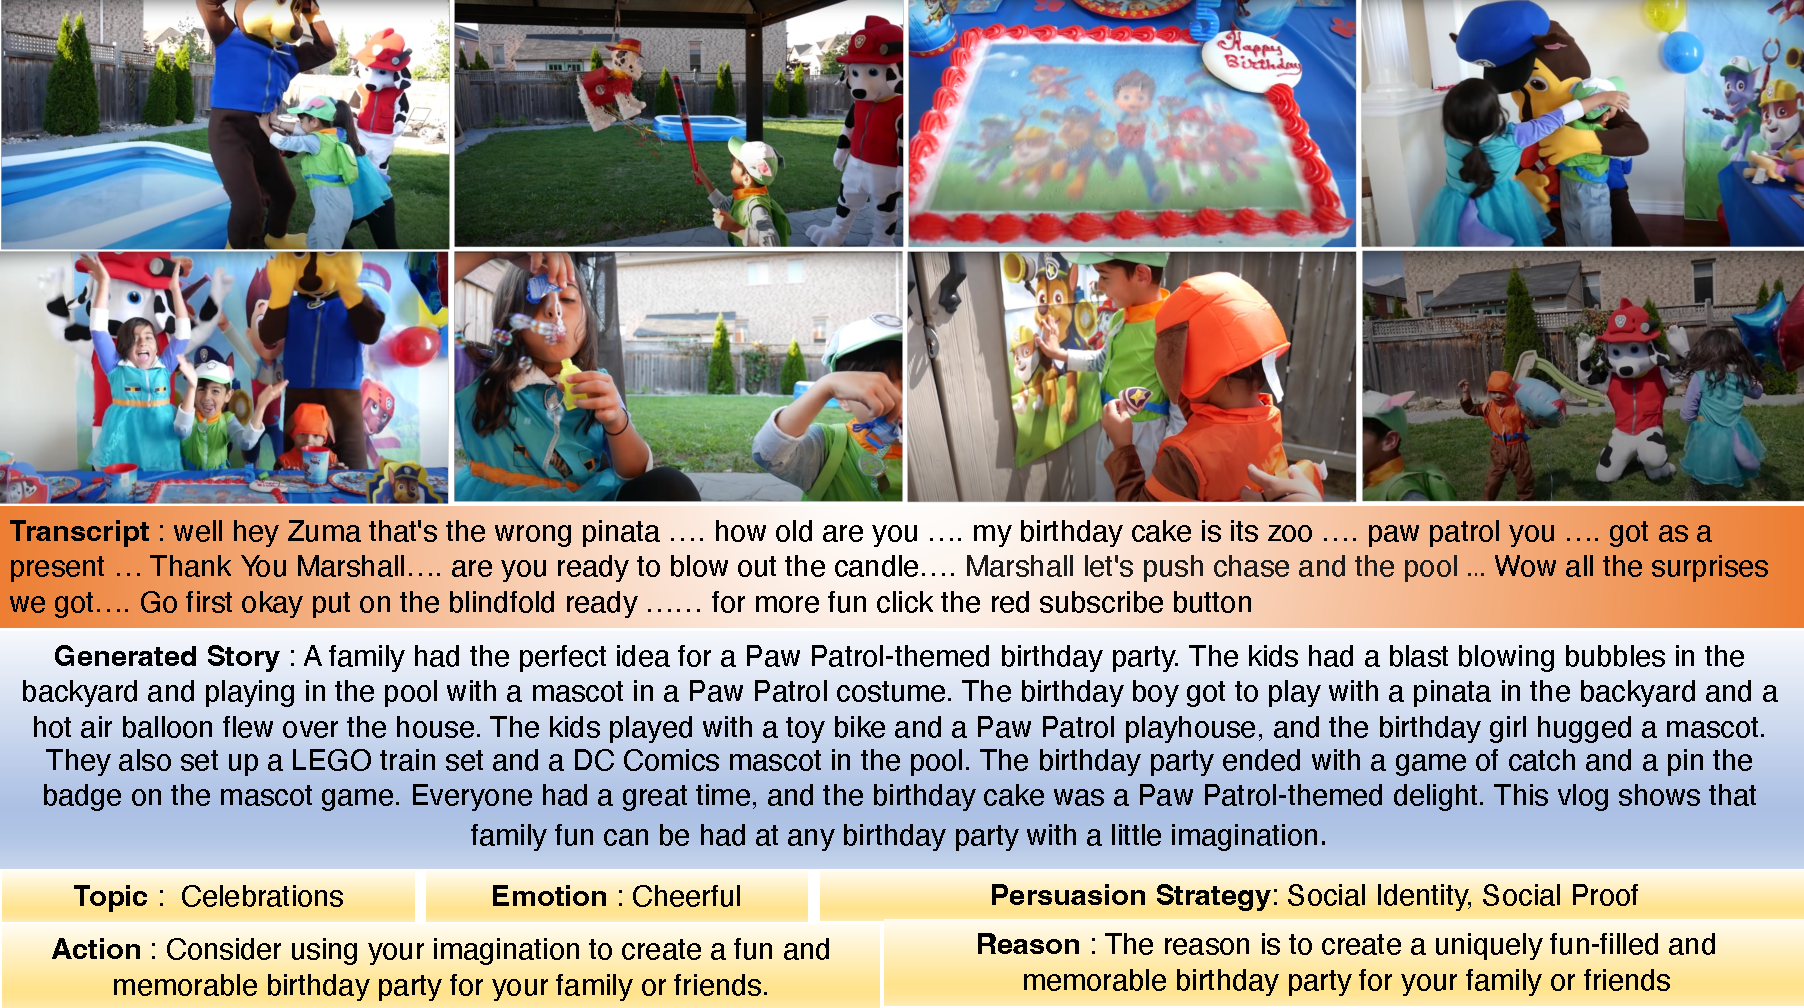
\includegraphics[width=\textwidth]{images/example-stories.pdf}
    \caption{An example of a story generated by the proposed pipeline along with the predicted outputs of the video-understanding tasks on the generated story. The generated story captures information across scenes, characters, event sequences, dialogues, emotions, and the environment. This helps the downstream models to get adequate information about the video to reason about it correctly. The original video can be watched at \url{https://youtu.be/_amwPjAcoC8}.}
    \label{fig:example-story}
\end{figure*}


\textit{b. Textual elements in frames:} We also extract the textual information present in the frames, as text often reinforces the message present in a scene and can also inform viewers on what to expect next \cite{9578608}. 
For the OCR module, we sample every 10th frame extracted at the native frames-per-second of the video, and these frames are sent to PP-OCR \cite{10.1145/2629489}. We filter the OCR text and use only the unique words for further processing.

\noindent \textbf{3. Text Representation of Audio:} The next modality we utilize from the video is the audio content extracted from it. We employ an Automatic Speech Recognition (ASR) module to extract transcripts from the audio. Since the datasets we worked with involved YouTube videos, we utilized the YouTube API to extract the closed caption transcripts associated with those videos.

\noindent \textbf{4. Prompting:} We employ the aforementioned modules to extract textual representations of various modalities present in a video. This ensures that we capture the audio, visual, text, and outside knowledge aspects of the video. Once the raw text is collected and processed, we utilize it to prompt a generative language model in order to generate a coherent story that represents the video. To optimize the prompting process and enable the generation of more detailed stories, we remove similar frame captions and optical character recognition (OCR) outputs, thereby reducing the overall prompt size. %\cy{Do we simply concantenate all the text as the prompt? in what order?}

The prompt template is given in Section~\ref{sec:prompt-format}. Through experimentation, we discovered that using concise, succinct instructions and appending the text input signals (such as frame captions, OCR, and automatic speech recognition) at the end significantly enhances the quality of video story generation. For shorter videos (up to 120 seconds), we utilize all available information to prompt the LLM for story generation. However, for longer videos, we limit the prompts to closed captions and sampled frame captions. The entire prompting pipeline is zero-shot and relies on pre-trained LLMs. In our story generation experiments, we employ GPT-3.5 \cite{brown2020language}, Flan-t5 \cite{chung2022scaling}, and Vicuna \cite{vicuna2023}. A temperature of 0.75 is used for LLM generation. The average length of the generated stories is 231.67 words. Subsequently, these generated stories are utilized for performing video understanding tasks.



\subsubsection{Prompt format} 
\label{sec:prompt-format}
 For verbalization, a template prompt format has been used, including all the data components as objects, captions, asr, ocr, meta-data. 

\textit{``Please write a coherent story based on the following video advertisement. Use only the information provided and make sure the story feels like a continuous narrative and at the end include one sentence about what product the advertisement was about. Do not include any details not mentioned in the prompt.Use the elements given below to create a coherent narrative,but don't use them as it is.The advertisement for the company \{company\_name\} The video is titled \{title\}, with captions that include \{caption\}, voice-over : \{transcripts\}, and object recognition descriptions : \{ocr\}. The following objects are present in the advertisement and should be used to help create the story: \{objects\} Please exclude any empty or stop words from the final text.''}

For downstream tasks, a template prompt format with an instruction about the specific task,the previous generated verbalization and vocabulary for the downstream task is prompted to the LLM. Here is the example for the topic detection task, for other tasks context and vocab were changed accordingly.

\textit{``Given \{topics\} identify the most relevant topic from the dictionary keys from topic\_vocab related to the story of the video advertisement given below.Consider the definitions given with topics in the topic\_vocab dictionary, to identify which topic is most relevant, don't add any extra topics that are not given in dictionary keys and answer with just the most relevant topic. Story : \{verbalization\}''}


\begin{table*}[!h]\centering
% \scriptsize
\begin{adjustbox}{width=\textwidth}
\begin{tabular}{llccccccc}\toprule[1.5pt]
\multirow{2}{*}{\textbf{Training}} & \multirow{2}{*}{\textbf{Model}} &\textbf{Topic} &\multicolumn{2}{c}{\textbf{Emotion}} & \textbf{Persuasion} &\textbf{Action} &\textbf{Reason}\\\cmidrule{4-5}
& & & \textbf{All labels} & \textbf{Clubbed} \\ \midrule[0.5pt]
Random & Random & 2.63 & 3.37 & 14.3 & 8.37 & 3.34 & 3.34 \\\hline
Finetuned & VideoMAE \cite{tong2022videomae} & 24.72 & 29.72 & \valgood{85.55}  & 11.17  & - & - \\
& Hussain \textit{et al.} \cite{hussain2017automatic} & 35.1 & 32.8 & -  & - & - & 48.45 \\
\ & Intern-Video \cite{wang2022internvideo} & 57.47 & \valbest{36.08} & \valbest{86.59} & 5.47 & 6.8 & 7.1 \\\hline
Zero-shot & VideoChat \cite{li2023videochat} & 9.07 & 3.09 & 5.1 &  10.28 & - & - \\

\hline
\textbf{Our Framework} & \makecell{GPT-3.5 Generated Story +\\GPT-3.5 Classifier} & 51.6 & 11.68 & 79.69 &  35.02 &  66.27 & 59.59 \\
Zero-shot & \makecell{GPT-3.5 Generated Story +\\Flan-t5-xxl Classifier} & \valgood{60.5} & 10.8 & 79.10 &  \valgood{33.41} &  \valbest{79.22} & \valbest{81.72} \\
& \makecell{GPT-3.5 Generated Story +\\Vicuna Classifier} & 22.92 & 10.8 & 67.35 & 29.6 & 21.39 & 20.89 \\
& \makecell{Vicuna Generated Story +\\GPT-3.5 Classifier} & 46.7 & 5.9 & 80.33 & 27.54 & 61.88 & 55.44 \\
& \makecell{Vicuna Generated Story +\\Flan-t5-xxl Classifier} & 57.38 & 9.8 & 76.60 & 30.11 & \valgood{77.38} & \valgood{80.66}  \\
& \makecell{Vicuna Generated Story +\\Vicuna Classifier} & 11.75 & 10.5 & 68.13 & 26.59 & 20.72 & 21.00  \\\cmidrule{2-8}
Finetuned & \makecell{Generated Story +\\Roberta Classifier} & \valbest{71.3} & \valgood{33.02} & 84.20 & \valbest{64.67} & 42.96\footnotemark[1] & 39.09\footnotemark[1] \\
% & BLIP-2 Captions + Flant-t5-xl & 32.2 & 7.4 & 43.11 &  32.1 & 52.98 & 76.26 \\
% & BLIP-2 Captions + GPT-3.5 & 32.7 & 7.9 & 76.3 & 30.1 & 49.91 & 58.71 \\

\bottomrule[1.5pt]
\end{tabular}
\end{adjustbox}
\caption{Comparison of all the models across topic, emotion, and persuasion strategy detection tasks. We see that our framework, despite being zero-shot, outperforms finetuned video-based models on the topic classification, persuasion strategy detection and action and reason classification tasks and comes close on the emotion classification task. Further, the Roberta classifier trained on generated stories outperforms both finetuned and zero-shot models on most tasks. Best models are denoted in \valbest{green} and runner-ups in \valgood{blue}.\label{tab:topic-sentiment}}
\end{table*}



\begin{table*}[!th]
  \centering
  % \begin{tabular}{cccccccccc}
  \begin{adjustbox}{width=\textwidth}
  \begin{tabular}{cccccccccc}
    \toprule
    & Method & Model Type & METEOR & CIDEr & ROUGE-L & BLEU-1 & BLEU-2 & BLEU-3 & BLEU-4 \\
    \midrule
    
    Random & Random  & Retrieval  & 13.1 & 30.2 & 21.4 & 43.1 & 23.1 & 10.0 & 4.8 \\\hline
    %\textbf{Finetuned} & CCA \cite{5540112} & Retrieval & 16.5 & 71.8 & 26.7 & 60.1 & 34.7 & 11.8 & 10.1 \\
    %& Uniform \cite{Li_2020}  & Retrieval & 18.3 &  89.9 & 28.0 & 65.7 & 40.6 & 23.2 & 13.2 \\
    %& SeqDPP \cite{NIPS2014_0eec27c4}  & Retrieval & 18.3 & 91.6 & 28.3 & 66.3 & 41.0 & 23.6 & 13.1 \\
    %& Submodular \cite{7298928} & Retrieval & 18.4 & 92.0 & 28.1 & 66.4 & 41.0 & 23.8 & 13.3 \\
    %& vsLSTM \cite{zhang2016video} & Retrieval & 18.2 & 92.4 & 28.2 & 66.6 & 41.5 & 24.1 & 13.6 \\
    %\textbf{Finetuned} & Narrator IoU \cite{Li_2020} & Retrieval & 18.6 & 93.7 & 28.2 & 67.9 & 42.1 & 24.7 & 14.1 \\
    %& Narrator w/o x \cite{Li_2020} & Retrieval & 18.5 & 93.4 & 28.3 & 67.3 & 41.6 & 24.5 & 14.2 \\
    %\textbf{Finetuned} & Narrator w/o f\_(l) \cite{Li_2020} & Retrieval & 19.0 & 96.1 & 29.1 & 68.6 & 42.9 & 25.2 & 14.5 \\
    \textbf{Finetuned} & Narrator \cite{Li_2020} & Retrieval & 19.6 & 98.4 & 29.5 & 69.1 & 43.0 & 25.3 & 15.0 \\
    %& \citet{xu2015show} & Retrieval & 17.7 & 79.5 & 28.0 & 61.7 & 36.4 & 20.2 & 11.5 \\
    %& m-RNN \cite{10.5555/2886521.2886647} & Retrieval & 18.0 & 81.3 & 28.5 & 61.9 & 37.0 & 21.1 & 11.8 \\
    & EMB \cite{Li_2020} & Retrieval & 19.1 & 88.8 & 28.9 & 64.5 & 39.3 & 22.7 & 13.4 \\
    & BRNN \cite{Li_2020} & Retrieval & 18.1 & 81.0 & 28.3 & 61.4 & 36.6 & 20.3 & 11.3 \\
    & ResBRNN \cite{Li_2020} & Retrieval & 19.6 & 94.3 & 29.7 & 66.0 & 41.7 & 24.3 & 14.7 \\
    & \makecell{Pseudo-GT+\\ResBRNN-kNN \cite{Li_2020}} & Retrieval & 20.1 & 103.6 & 29.9 & 69.1 & 43.5 & 26.1 & 15.6 \\
    & GVMF \cite{https://doi.org/10.1049/ell2.12525} & Retrieval & 20.7 & \valgood{107.7} & \valbest{30.8} & \valbest{70.5} & 44.3 & 26.9 & 15.9 \\    \hline
    %& S2VT \cite{venugopalan2015sequence}  & Generative & 14.3 & 64.0 & 28.6 & 63.3 & 40.6 & 24.6 & 15.4 \\
    %& H-RNN \cite{yu2017hierarchicallyattentive} & Generative & 15.5 & 64.6 & \valgood{28.8} & 61.6 & 41.4 & 26.3 & 16.1 \\
    \textbf{Zero-shot} & VideoChat \cite{li2023videochat} & Generative & 15.49 & 42.9 & 17.88 & 50.00 & 43.30 & 34.76 & 27.21 \\\hline
    
   \textbf{\makecell{Zero-shot}} & GPT-3.5 & Generative & \valbest{24.8} & 102.4 & 24.3 & \valgood{63.8} & \valgood{56.4} & \valgood{47.2} & \valbest{38.6} \\
    Our Framework & Vicuna & Generative & 17.4 & 73.9 & 20.9 & \valbest{70.49 }& \valbest{60.0} & \valbest{48.25} & \valgood{38.20} \\
    & Flant-t5-xxl & Generative & 4.8 & 34.6 & 10.58 & 7.9 & 6.8 & 5.4 & 4.3 \\
    & \makecell{Uniformly Sampled\\BLIP-2 Captions} & Generative & \valgood{21.7} & \valbest{108.9} & 24.04 & 55.19 & 48.5 & 40.7 & 33.76 \\%\cline{2-10}

    \bottomrule
  \end{tabular}
  \end{adjustbox}
  \caption{Comparison on story generation task on the video-story dataset. We see that our framework despite being zero-shot outperforms all the fine-tuned generative prior art on all metrics. Further, it also outperforms fine-tuned retrieval models, which choose from a fixed set of frame descriptions on most metrics. Best models are denoted in \valbest{green} and runner-ups in \valgood{blue}. \label{tab:story-generation}}
\end{table*}




\begin{table*}[!h]
\centering
% \begin{tabular}{cccccccccc}
\begin{adjustbox}{max width=\textwidth}
\begin{tabular}{ccccccccc}
\toprule
Task & Model & METEOR & CIDEr & ROUGE-L & BLEU-1 & BLEU-2 & BLEU-3 & BLEU-4 \\
\midrule
Action & GPT-3.5  & \valbest{20.46} & 41.7 & 9.5 & 18.7 & 14.8 & 11.8 & 9.4 \\
Action & Flan-t5-xxl & 15.75 & \valbest{61.5} & \valbest{13.6} & \valbest{50.0} & \valbest{34.8} & \valbest{26.9} & \valbest{21.8} \\
Action & Vicuna & 21.20 & 42.6 & 7.6 & 16.8 & 13.08 & 10.08 & 7.7 \\
\hline
Reason & GPT-3.5 & 13.34 & 16.7 & \valbest{7.8} & 27.1 & 20.8 & 14.7 & 10.4 \\
Reason & Flan-t5-xxl & 8.35 & 24.9 & 5.9 & \valbest{39.4} & \valbest{24.7} & \valbest{16.7} & \valbest{12.0 }\\
Reason & Vicuna & \valbest{15.82} & \valbest{27.9} & 7.75 & 24.6 & 19.3 & 14.1 & 10.3 \\
\hline
Reason given action & GPT-3.5 & \valbest{13.77} & \valbest{29.4} & \valbest{8.7} & \valbest{33.5} & \valbest{24.9} & \valbest{17.9} & \valbest{13.2} \\
Reason given action & Flan-t5-xxl & 4.29 & 19.0 & 7.6 & 23.2 & 15.0 & 10.2 & 7.5 \\
Reason given action & Vicuna & 13.62 & 24.4 & 7.61 & 22.6 & 17.7 & 12.8 & 9.2 \\

\bottomrule
\end{tabular}
\end{adjustbox}
\caption{Comparison of the different zero-shot models on the action and reason generation tasks. Note that there are no fine-tuned generative models in the literature for this task and the number of annotated videos is too small to train a generative model. Best models are denoted in \valbest{green}. \label{tab:action-reason-generation}}
\end{table*}




\begin{table*}[!tp]
\centering
\begin{adjustbox}{max width=1.0\textwidth}
\begin{tabular}{llccccccccc}
\toprule[1.5pt]
\textbf{Training} & \textbf{Model} & \textbf{relationship} & \textbf{way\_speaking} & \textbf{scene} & \textbf{like\_ratio} & \textbf{view\_count} & \textbf{director} & \textbf{genre} & \textbf{writer} & \textbf{year} \\
\midrule[0.5pt]
Trained & R101-slowfast+NL \cite{wu2021towards} & 52.4 & 35.8 & 54.7 & 0.386 & \valgood{3.77} & 44.9 & 53.0 & 36.3 & 52.5 \\
Trained & VideoBert \cite{sun2019videobert} & 52.8 & 37.9 & 54.9 & 0.320 & 4.46 & 47.3 & 51.9 & 38.5 & 36.1 \\
Trained & Xiao \textit{et al.} \cite{xiao2022hierarchical} & 50.95 & 34.07 & 44.19 & 0.353 & 4.886 & 40.19 & 48.11 & 31.43 & 29.65 \\
Trained & Qian \textit{et al.} \cite{qian2021spatiotemporal} & 50.95 & 32.86 & 32.56 & 0.444 & 4.600 & 37.76 & 48.17 & 27.26 & 25.31 \\
Trained & Object Transformers \citep{wu2021towards} & 53.1 & \valbest{39.4} & 56.9 & 0.230 & \valbest{3.55} & 51.2 & \valgood{54.6} & 34.5 & 39.1 \\ 
\hline
\makecell{Zero-shot\\(Ours)} & \makecell{GPT-3.5 generated\\story + Flan-t5-xxl} & \valgood{64.1} & \valgood{39.07} & \valgood{60.2} & 0.061 & 12.84 & \valgood{69.9} & \valbest{58.1} & \valbest{52.4} & \valgood{75.6} \\
\makecell{Zero-shot\\(Ours)} & \makecell{GPT-3.5 generated\\story + GPT-3.5 classifier} & \valbest{68.42} & 32.95 & 54.54 & \valbest{0.031} & 12.69 & \valbest{75.26} & 50.84 & 32.16 & \valbest{75.96} \\
\hline
\makecell{Trained\\(Ours)} & \makecell{GPT-3.5 generated\\story + Roberta} & 62.16 &  38.41 &  \valbest{68.65} &\valgood{0.054} & 11.84 & 45.34 & 39.27 & \valgood{35.93} & 7.826 \\
\bottomrule[1.5pt]
\end{tabular}
\end{adjustbox}
\caption{Comparison of various models on the LVU benchmark. We see that our framework, despite being zero-shot, outperforms fine-tuned video-based models on 8/9 tasks. Best models are denoted in \valbest{green} and runner-ups in \valgood{blue}.}
\label{table:lvu-results}
\end{table*}
\begin{table*}[!tp]
\centering
\begin{adjustbox}{max width=1.0\textwidth}
\begin{tabular}{llcccccccc}
\toprule[1.5pt]
\textbf{Training} & \textbf{Model} & \textbf{Scene} & \textbf{Object} & \textbf{Action} & \textbf{Event} & \textbf{Attribute} & \textbf{Concept} & \textbf{Overall} \\
\midrule[0.5pt]
Trained & 3D-Resnet & 50.6 & 28.6 & 48.2 & 35.9 & 29 & 22.5 & 35.8 \\
Trained & 3D-STCNet & 51.9 & 30.1 & 50.3 & 35.8 & 29.9 & 22.7 & 36.7 \\
Trained & HATNet & 55.8 & 34.2 & 51.8 & 38.5 & 33.6 & 26.1 & 40 \\
Trained & 3D-Resnet (Multitask) & 51.7 & 29.6 & 48.9 & 36.6 & 31.1 & 24.1 & 37 \\
Trained & HATNet (Multitask) & 57.2 & 35.1 & 53.5 & \valgood{39.8} & 34.9 & 27.3 & 41.3 \\
\hline
\makecell{Zero-shot\\(Ours)} & \makecell{GPT-3.5 generated story\\ + Flan-t5-xxl classifier}  & \valgood{59.66} & \valgood{98.89} & \valbest{98.96} & 38.42 & \valbest{67.76} & \valgood{86.99} & \valgood{75.12} \\
\makecell{Zero-shot\\(Ours)} & \makecell{GPT-3.5 generated story\\ + GPT-3.5 classifier} & \valbest{60.2} & \valbest{99.16} & \valgood{98.72} & \valbest{40.79} & \valgood{67.17} & \valbest{88.6} & \valbest{75.77} \\
\bottomrule[1.5pt]
\end{tabular}
\end{adjustbox}
\caption{Comparison of various models on the HVU benchmark \cite{diba2020large}. The models scores are as reported in \cite{diba2020large}. We see that our framework, despite being zero-shot, outperforms fine-tuned video-based models on all the tasks. Best models are denoted in \valbest{green} and runner-ups in \valgood{blue}.}
\label{table:hvu-benchmark}
\end{table*}


\subsubsection{Results}


\textbf{Video Storytelling:} The performance comparison between our pipeline and existing methods is presented in Table~\ref{tab:story-generation}. We evaluate multiple generative and retrieval-based approaches and find that our pipeline achieves state-of-the-art results. It is important to note that as our method is entirely generative, the ROUGE-L score is lower compared to retrieval-based methods due to less overlap with ground truth reference video stories. However, overall metrics indicate that our generated stories exhibit a higher level of similarity to the reference stories and effectively capture the meaning of the source video.


\textbf{Video Understanding:} The performance comparison between our pipeline and other existing methods across six tasks (topic, emotion, and persuasion strategy classification, as well as action and reason retrieval and generation) is presented in Tables~\ref{tab:topic-sentiment} and \ref{tab:action-reason-generation}. Notably, our zero-shot model outperforms finetuned video-based baselines in all tasks except emotion classification. Further, our text-based finetuned model outperforms all other baselines on most of the tasks.

Unlike the story generation task, there are limited baselines available for video understanding tasks. Moreover, insufficient samples hinder training models from scratch. To address this, we utilize state-of-the-art video understanding models, VideoMAE and InternVideo. InternVideo shows strong performance on many downstream tasks. 
%We enhance them by adding two linear classification layers and a pooling layer on top and train it with a sampling rate of 2 frames per second.
Analyzing the results, we observe that while GPT-3.5 and Vicuna perform similarly for story generation (Table~\ref{tab:story-generation}), GPT-3.5 and Flan-t5 excel in downstream tasks (Table~\ref{tab:topic-sentiment}). Interestingly, although GPT-3.5 and Vicuna-generated stories yield comparable results, GPT-3.5 exhibits higher performance across most tasks. Vicuna-generated stories closely follow GPT-3.5 in terms of downstream task performance.


Next, we compare the best models (as in Table~\ref{tab:topic-sentiment}) on the LVU and HVU benchmarks with respect to the state-of-the-art models reported in the literature. Tables~\ref{table:lvu-results} and \ref{table:hvu-benchmark} report the results for the comparisons. As can be noted, the zero-shot models outperform most other baselines. For LVU, the zero-shot models work better than the trained Roberta-based classifier model. For HVU, we convert the classification task to a retrieval task, where in a zero-shot way, we input the verbalization of a video along with 30 randomly chosen tags containing an equal number of tags for each category (scene, object, action, event, attribute, and concept). The model is then prompted to pick the top 5 tags that seem most relevant to the video. These tags are mapped back to the main category tags, which are treated as the predicted labels. 


Furthermore, as a comparative and ablation study of our approach, we evaluate the performance using only the BLIP-2 captions and audio transcriptions (Table~\ref{tab:ablation-topic-sentiment}). Our findings highlight that generated stories leveraging both audio and visual signals outperform those using vision or audio inputs alone. This emphasizes the significance of verbalizing a video in enhancing video understanding.



\subsubsection{Ablation}
Among the different components of information input present in the prompt, the LLM utilizes them differently while constructing the verbalization for the videos.For this experiement we use a subset of \cite{hussain2017automatic} dataset, considering videos that have spoken audio present.

We use ROUGE-l to get the longest common subsequence (LCS) between the generated verbalization and the individual components,which captures the overlapping content, providing an indication of their semantic similarity.

As generated verbalizations are abstractive as compared to extractive, we also use cosine similarity between the Roberta embeddings of the generated verbalization and the individual components.

We find that despite the order of the components in the prompt, the LLMs tend to utilize the audio components in the videos, in an extractive way. 



\begin{table*}[!tp]\centering
% \scriptsize
\begin{adjustbox}{max width =\textwidth}
\begin{tabular}{llcccccc}\toprule[1.5pt]
\multirow{2}{*} & \multirow{2}{*}{\textbf{Model}} &\textbf{Topic} &\multicolumn{2}{c}{\textbf{Emotion}} & \textbf{Persuasion} &\textbf{Action} &\textbf{Reason}\\\cmidrule{4-5}
& & & \textbf{All labels} & \textbf{Clubbed} \\ \midrule[0.5pt]
& BLIP-2 Captions + Flant-t5-xxl & 32.2 & 7.4 & 43.11 &  32.1 & 52.98 & 76.26 \\
& BLIP-2 Captions + GPT-3.5 & 32.7 & 7.9 & 76.69 & 30.1 & 49.91 & 58.71 \\
& Audio Transcription + Flant-t5-xxl &  49.37 & 10.1 & 63.56 &  21.9 & 66.17 & 79.68 \\
& Audio Transcription + GPT-3.5 & 32.88 & 6.4 & 75.97 & 32.25 & 64.98 & 61.78 \\

\bottomrule[1.5pt]
\end{tabular}
\end{adjustbox}
\caption{Ablation study of using only visual (caption) or audio (transcripts) and LLMs for downstream tasks. It can be noted that the overall model does not perform as well (compared to Table~\ref{tab:topic-sentiment}) when using only audio or scene description without generating story. \label{tab:ablation-topic-sentiment}}
\end{table*}


\begin{table*}[!h]
\centering
\begin{adjustbox}{max width=0.8\textwidth}
\begin{tabular}{ccc}
\toprule
Model & Top-5 Accuracy & mAP \\
\midrule
VideoMAE & 25.57 & 24.79 \\
InternVideo & 7.477 & 15.62 \\
GPT-3.5 Generated Story + GPT-3.5 & 34.2 & 27.53 \\
Vicuna Generated Story + GPT-3.5 & 31.54 & 27.24 \\
GPT-3.5 Generated Story + Flant5 & 37 & 27.96 \\
Vicuna Generated Story + Flant5 & 31.13 & 27.32 \\
\bottomrule
\end{tabular}
\end{adjustbox}
\caption{Top-5 accuracy, and mAP for persuasion strategy detection task}
\end{table*}





\subsubsection{A few examples of the stories generated using our method}
\label{sec:examples-stories-generated}
    \noindent1.~``Cathy 30 Master'' by Grand Canyon University (\url{https://www.youtube.com/watch?v=lPdD8NvVfw0}): 
    Kathy Ames had always wanted to pursue a doctoral degree but was unsure about the time commitment. When she discovered Grand Canyon University, she knew she had found the perfect fit. Grand Canyon University offered a flexible schedule that would allow her to balance her personal and family life with her studies. She - along with other students - gathered in the classroom, excitedly listening to their coach, Scott Saunders, explain the program. Afterward, Kathy made her way to the library and settled into a chair with her laptop. 
    
    She studied diligently, surrounded by her peers and classmates. In the evenings, she met with her peers around the table to discuss the topics of the day. Everyone was always eager to help and support each other. After a long day, Kathy made her way back to her living room where she relaxed on the couch with a glass of water and a lamp providing a soothing light. 
    
    Kathy was grateful for the opportunity to pursue her dream at Grand Canyon University. She was able to learn from experienced faculty and gain real-world experience that would prepare her for success after graduation. 
    
    The advertisement for Grand Canyon University was about offering a private, Christian education at an affordable price.


    \noindent2.~``Today is the Day for Doing | The Home Depot'' by Home Depot (\url{https://www.youtube.com/watch?v=f_6QQ6IVa6E}): The woman holding the book stepped onto the patio and looked up to the sky. She was ready to take on the day. Taking out her phone, she opened the furniture catalog app, scrolling through the various designs. She quickly decided on the perfect pieces to brighten up her home. Next, she headed to The Home Depot for the supplies she needed. As she entered the store, the woman was delighted to find all the tools and materials she needed, from the Ryobi Cordless Vacuum to the Leaf Blower. She was even more excited when she spotted the Splatter an object recognition tool that allowed her to easily find the perfect paint color for her project. With her shopping done, the woman made her way to the checkout line with a cup of coffee in hand. She couldn't wait to get to work and make her home more beautiful. She knew that with the help of The Home Depot, Today was the Day for Doing. This advertisement was for The Home Depot - the one-stop-shop for all your home improvement needs. \\


    

    \noindent3.~``October 2018 Color of the Month: Shell White - Sherwin-Williams'' by Sherwin-Williams (\url{https://www.youtube.com/watch?v=PJlHiQJBDMw}): The advertisement for the company Sherwin-Williams opens on a kitchen table strewn with shells and wicker baskets, with two glasses of iced water beside them. A vase with a blue pattern sits in the foreground, and a person holds up a phone with the Sherwin-Williams logo on the screen. A girl appears from behind a white sheet, peeking out of a white tent as if to signify the timelessness and neutrality of this color. The voice-over begins, as the camera pans to a living room with a staircase, and then to a dining room with a white table, chairs, and a white vase. The words ``Color of the Month: Shell White, Sherwin-Williams" appear on the screen, as the camera zooms in on the vase. The words are followed by \"Our app makes it a snap,\" referring to Color Snap, the company's new way of painting a home. The advertisement ends with the Sherwin-Williams logo, emphasizing the company's commitment to excellence in home painting. This advertisement was promoting the company's color of the month, Shell White. \\

    \noindent4.~``Side-by-side comparison of SolidWorks w/NVIDIA Quadro FX 1700 vs. Quadro 2000'' by NVIDIA (\url{https://www.youtube.com/watch?v=CDjBIt70fp4}): The story began with a green light glowing in the dark, symbolizing the presence of a powerful technology that can change the way we work. This technology was an advanced graphics card, the NVIDIA Quadro FX 1700. It was compared side-by-side with its successor, the Quadro 2000, and it was clear that the Quadro 2000 was far more powerful. The Quadro FX 1700 had a qt - x700 vs qt - x700 capacity, while the Quadro 2000 had a green light that shone brighter and further than before. As the comparison was being made, the results were clear: the Quadro 2000 was the superior product. This advertisement for the company NVIDIA showcased the power of the Quadro 2000, and the improved performance it could bring to an organization. The advertisement concluded with a green light, signaling that NVIDIA had the answer to improving workflows. The product the advertisement was about was the NVIDIA Quadro 2000." \\

    

    \noindent5.~``Training sessions in the nature - Mary Kom | Priyanka Chopra | In Cinemas NOW'' by Viacom 18 Studios (\url{https://www.youtube.com/watch?v=SXTSJC5NrLs}): Mary Kom was training hard to make her mark as a boxer, and she had nothing but her focus and determination to help her succeed. She was a force to be reckoned with in the boxing ring and her hard work was soon paying off.But she knew that she had to take her training to the next level if she wanted to win the boxing championship. That's when she decided to take her own advice and step out of her comfort zone. She headed out to the woods, determined to make the most of her time in nature.The woods were a perfect place for Mary to challenge herself physically. She was soon standing on the rocks of a river, pushing her body to its limits with every movement. She was standing tall, her black top glinting in the sunlight, and her energy was palpable. The sun was setting, and it was the perfect time to relax and unwind.Finally, she ended her day with a yoga routine, her body twisting and turning in a beautiful display of strength and grace. It was a day of hard work and fun, and it left Mary feeling inspired and ready to take on anything. The video was an advertisement for the movie Mary Kom, released by Viacom18 Studios." \\


\subsubsection{Hallucinations Present In the Automatically Generated Stories}

The current large language models , do hallucinate or produce imaginary outputs. However, they are able to capture the gist of the videos, helping improve on downstream tasks. Some examples are shown below:

\begin{enumerate}
    \item ``The Fundamentals Of Caring | Clip: "Perverts" | Netflix'' by Netflix (\url{https://youtu.be/_Usyxm9S_Jg})
    \begin{enumerate}
        \item Story: The woman in the advertisement is standing in front of a red background, smiling brightly. She and a man sitting at a table look content, as if they've just come from a conversation. The Netflix logo is visible, indicating that the advertisement is for the company and its products. The voice-over for the advertisement introduces Selena Gomez as the star of the trailer for the popular Twilight Saga. Her popularity has made her a perfect choice to promote Netflix's products. The voice-over then informs viewers that the company's streaming service is not available. The man and woman in the advertisement seem to have a strong connection, and we can infer that they are friends. Perhaps they share an understanding of each other's struggles, since they both seem to be comfortable and happy with each other. The advertisement ends with the Netflix logo, leaving viewers with the knowledge that they can find solace and understanding in the company's products, no matter what they are going through. The advertisement was for Netflix."

        \item Hallucinations: The story falsely attributes ``Selena Gomez'' to ``Twilight Saga". The LLMs often confuse named entity linkages.
    \end{enumerate}

    \item ``Back-to-School 2016'' by Academy Sports + Outdoors (\url{https://youtu.be/SZwWT5lnHf8}) 
    \begin{enumerate}
        \item Story: A young girl is walking through her bedroom when she notices a man running up the stairs in his sneakers. She is intrigued and follows him, curious to see where he is going. Arriving at the top of the stairs, she finds a young man standing with his backpack. Across the room, she sees a girl in a dress standing in front of a mirror. The girl smiles and looks content. At that moment, the voice-over of the Academy Sports + Outdoors ad can be heard: "Academy Sports and Outdoors is the place to get all the best brands in thousands of combinations for back to school. Right stuff, low price, every day." Suddenly, a black cat can be seen flying in the sky and the girl in the tank top is now standing in front of the mirror. The man is wearing blue pants and sneakers, and the shoes, rug, and sneakers of the apartment are visible. The girl smiles and looks content. The scene shifts to the bedroom where the bed, dresser, and mirror are present, along with a sign for Academy Sportswear. This advertisement for Academy Sports + Outdoors was about the company's back-to-school collection of products. It showcased how Academy Sports + Outdoors provides the right stuff, at a low price, every day, for students to get ready for school.

        \item The scene with a black cat is hallucinated though not mentioned in the prompt

    \end{enumerate}
    
    \item ``Many Worlds, One Home l Anime 2019 l NX'' By Netflix (\url{https://youtu.be/B63ubKGNqos}) 
    \begin{enumerate}
        \item Story: The advertisement by Netflix, titled "Many Worlds, One Home", is a stunning vision of many different universes. We see a man standing on a red moon, a desert landscape, and a live performance by Adam Sandler. Purple backgrounds with the word "worlds" convey the idea of many possibilities, while a boy playing with a ball in front of a statue shows a more peaceful and homely side to this. As the night falls, a man is standing on a car, and the Ultraman. There are also glimpses of Tse Seeds, Devilman Crybaby, Saint Seiya: Knights of the Zodiac, Eden Vs. Eden, Carole and Tuesday, Aggretsuko, Seis Manos, Godzilla, Castlevania, B: The Beginning, Baki, Cannon Busters, Rilakkuma and Kaoru, Beastars, and Ultramarine Magmell. We see a teddy bear, knights of the zodiac, a character walking in the water, a man in a snowy area, a pair of shoes, a man running away from the fire, the moon, a man wearing a suit with a green light, eyes being the only thing that can be seen, birds flying in the sky, a red and black background with a red light, bats and castles, the eyes, a man holding a gun, a man flying in the air, a face, a girl with long hair, and two hands. All of this culminates to signify the many different worlds that one can find "home", and the advertisement concludes with the Netflix logo. This advertisement for Netflix captures the idea of many possibilities and of being at home in a single place.
        
        \item Hallucination: Blip2 hallucinates entities such as ``Adam Sandler'' who is not associated with the advertisement. But it causes the generated story to have the same association.
    \end{enumerate}
    
    

    \item ``African Cats: Herding Cats - Clip'' by Walt Disney Studios (\url{https://youtu.be/WCIEmrN8ot4}) 
    \begin{enumerate}
        \item Story: The sun shone brightly in the savanna as the cheetah cub frolicked in the grass. Suddenly, a cheetah emerged from the shadows. The cheetah and it's cub plan to chase the gazzeles. Despite the presence of death, life in the wild continued on, just as it had for centuries. This story is featured in the advertisement for Walt Disney Studios, which captures the beauty and unpredictable nature of life in the African savanna. This advertisement ultimately serves to promote the film African Cats, which tells the story of a cheetah family as they strive to protect their respective prides against a variety of obstacles in the wild.
        
        \item Hallucination: The generated caption ``a fox cub is playing in the grass cheetah eats in the wild" was insufficient to capture the overall information of the video, however, due to the presence of ASR and world knowledge of the LLM. The LLM is able to generate a coherent story. 
    \end{enumerate}

        \item ``Bright \& Dreamy: Pastel Tint| Ulta Beauty'' by ultabeauty (\url{https://youtu.be/Lh5n4HcLvCU}) 
        \begin{enumerate}
            \item Story: The woman in the Ulta Beauty advertisement skillfully applied makeup to her face, creating a beautiful pastel tint. With each brush stroke, her look became brighter and more dreamy. She beamed with confidence and joy, her face glowing with beauty. As the advertisement continued, she highlighted her eyes and cheeks with subtle pastel shades, adding to the stunning effect. With each addition, her face lit up with a vibrant luminosity. When she was finished, her face was a work of art, the perfect combination of bright and dreamy. The Ulta Beauty advertisement showcased the power of a perfect pastel tint, and how it can enhance any look. This advertisement was for Ulta Beauty.

            \item Hallucination: The video contains only music. However, the generated verbalization can pick the advertisement's gist. 
        \end{enumerate}
        
        \item ``Round Brilliant Diamond Hoop Earrings 14kt White Gold'' by Costco \url{https://youtu.be/VdhRmVnbqQo} 
        \begin{enumerate}
            \item Story: Jackie had been wanting diamond hoop earrings for what seemed like forever. She had been dreaming of the perfect pair that she could wear on special occasions and that would bring out the best in her. One day Jackie happened to come across an advertisement for Costco, which featured a pair of Round Brilliant Diamond Hoop Earrings in 14kt White Gold. She immediately knew this was the perfect pair for her. The advertisement had a voice-over that said, “These earrings sparkle with glamour and sophistication." Jackie was mesmerized by the sparkle of the diamonds, and she was sure anyone who saw them would also be taken in by their beauty. Jackie quickly decided to purchase the earrings. She was sure they would make the perfect accessory for any special occasion. From date nights to family gatherings, she knew these earrings would make her look simply stunning. The advertisement for the Costco Round Brilliant Diamond Hoop Earrings in 14kt White Gold proved to be the perfect choice for Jackie. They not only added a touch of glamour and sophistication to her wardrobe, but made her feel extra special when she wore them. The advertisement for the company Costco was for a pair of Round Brilliant Diamond Hoop Earrings in 14kt White Gold.
            
            \item Hallucination: The video has no audio transcription, and minimal visual information. However the LLM hallucinates a story, maintaining the essence of the advertisement. It also attributes a false voice-over which is not present in the video.
        \end{enumerate}


    
\end{enumerate}



        
       

\section{Conclusion}
\textit{What does an advertisement say that makes people change their beliefs and actions?} With limited works, the computational study of rhetoric of this all-pervasive form of marketing communication is still in its infancy. In this chapter, based on the well-developed social psychology and marketing literature, we develop and release the largest vocabulary of persuasion strategies and labeled dataset. We develop several models for predicting persuasion strategies for video and image based ads. Further, we show the performance of these models on several other advertisement-understanding related tasks, including topic, emotion, and question-answering.





% \begin{figure}[t]
%         \centering
%         \includegraphics[scale =0.4]{images/company_sector-strategies.pdf}
%         \caption{Dice correlation between company sectors and strategies. Companies are taken from the Meta advertisement data and further these companies are labeled according to which sector they belong.}
%         \label{fig:correlation-between-company-sector-and-strategies}
%         % \vspace*{-3mm}
%     \end{figure}
    

% \begin{figure}[t]
%         \centering
%         \includegraphics[scale =0.5
%         ]{images/strategies-age_group.pdf}
%         \caption{correlation between age-group and top 6 strategies on the basis of frequency. Age-groups are taken from the Meta advertisement data.}
%         \label{fig:correlation-between-age-strategies}
%         % \vspace*{-3mm}
%     \end{figure}
    

% \begin{figure}[t]
%         \centering
%         \includegraphics[scale =0.55]{images/strategies-gender.pdf}
%         \caption{correlation between Gender and strategies.}
%         \label{fig:correlation-between-gender-and-strategies}
%         % \vspace*{-3mm}
%     \end{figure}

\begin{comment}
    \begin{figure}[t]
            \centering
            \includegraphics[scale =0.5]{images/correlation_sector_strategies.pdf}
            \caption{Dice correlation between company sectors and strategies.}
            \label{fig:correlation-between-company-sector-and-strategies}
            % \vspace*{-3mm}
    \end{figure}
\end{comment}

    
% \begin{figure*}
%         \centering
%         \begin{subfigure}[b]{0.75\textwidth}\centering
%         \includegraphics[scale=0.8]{images/us_heatmap_1.pdf}
%         \caption{US Heat Maps}
%         \end{subfigure}
%         % \vspace*{-3mm}
%     \end{figure*}
%     \begin{figure*}\ContinuedFloat
%         \centering
%         \begin{subfigure}[b]{0.75\textwidth}\centering
%         \includegraphics[scale=0.8]{images/us_heatmap_2.pdf}
%         \caption{US Heat-Maps}
%         \end{subfigure}
%         % \vspace*{-3mm}
%         \label{fig:us-heatmaps}
%     \end{figure*}

% \begin{table}[]
%         \centering
%         \begin{tcolorbox}[tab1,tabularx={YYYYY}]
%                 \toprule
%                 \textbf{\thead{Train \\Sample\\size}} & \textbf{\thead{Top-1 \\Accuracy}} & \textbf{\thead{Top-3 \\Accuracy}} &  \textbf{Recall} & \textbf{Precision} \\ \midrule
%                  1000 & 49.6 & 70.4 & 57.42 & \\ \midrule
%                  1250 & 50 &  73.2 & 59.07 & \\ \midrule
%                  1500 & 50.8 & 74.4 & 60.71 & \\ \midrule
%                  1750 & 50.8 & 76.4 & 62.36 & \\ \midrule
%                  2000 & 50 & 78 & 63.74 & \\ \midrule
%                  2250 & 50 & 75.6 & 63.74 & \\ \midrule
%                  2500 & 50.9 & 73.6 & 61.54 & \\\midrule
%         \end{tcolorbox}
%         \caption{Strategy prediction results on validation set}
%         \label{tab:my_label}
%     \end{table}
    
% \begin{table}[]
%         \centering
%         \begin{tcolorbox}[tab1,tabularx={YYYYY}]
%                 \toprule
%                  \textbf{\thead{Train \\Sample\\size}} & \textbf{\thead{Top-1 \\Accuracy}} & \textbf{\thead{Top-3 \\Accuracy}} &  \textbf{Recall} & \textbf{Precision} \\ \midrule
%                  1000 & 44 & 74.4 & 61.69 & 35.6 \\ \midrule
%                  1250 & 48.8 & 77.6 & 62.35 & 34.9\\ \midrule
%                  1500 & 52 & 76.4 & 62.00& 36.7 \\ \midrule
%                  1750 & 54.4 & 80.4 & 65.32 & 38.08 \\ \midrule
%                  2000 & 55.2 & 80.8 & 69.88 & 38.7\\ \midrule
%                  2250 & 58 & 80.8 & 72.06&40.00 \\ \midrule
%                  2500 & 59.2 & 84.8 & 74.59 &40.88 \\\bottomrule
%         \end{tcolorbox}
%         \caption{Strategy prediction results on test set}
%         \label{tab:my_label}
%     \end{table}
    


% \begin{table}[]
%     \small
%         \centering
%         \toprule
%         %\begin{adjustbox}{width=\columnwidth,center}
%         \resizebox{\columnwidth}{!}{%
%       \begin{tabular}{lll}%[tab1,tabularx={XYYYYY}]
%              \textbf{\thead{Models}} & \textbf{\thead{Top-1  Accuracy}} & \textbf{\thead{Top-3 Accuracy}}\\ \midrule
%              Our Model & 59.2 & 84.8 \\ \midrule
%              Without DenseCap & 55.6 & 80.8 \\ \midrule
%              Without Symbol   & 58.8 & 81.6 \\ \midrule
%           Without DenseCap\\\& Symbol & 55.2 & 80.8 \\ \midrule
%             Without OCR & 54.8 & 82 \\ \midrule
%             Without Symbol,\\OCR \& DenseCap & 58 & 78.8 \\ \midrule
%                  With Topic & 43.2 & 67.2 \\ \bottomrule
%         \end{tabular}}
%         \caption{\small  Effect of excluding different Modalities}
%         \vspace*{-3mm}
%         %\end{adjustbox}
%     \end{table}

%\begin{figure}[t]
%        \centering
%        \includegraphics[scale =0.2]{images/RandomSelection_vs_ActiveLearning.pdf}
%        \caption{Active Learning vs Random Selection}        \label{fig:AL_batch_test_discard}
%    \end{figure}





%%%%%%%%%%%%%%%%%%%%%%%%%%%%%%%%%%%%%%%%
%%%%%%%%%%%%%%%%%%%%%%%%%%%%%%%%%%%%%%%%
%%%%%%%%%%%%%%%%%%%%%%%%%%%%%%%%%%%%%%%%
%%%%%%%%%%%%%%%%%%%%%%%%%%%%%%%%%%%%%%%%
%%%%%%%%%%%%%%%%%%%%%%%%%%%%%%%%%%%%%%%%
%%%%%%%%%%%%%%%%%%%%%%%%%%%%%%%%%%%%%%%%
%%%%%%%%%%%%%%%%%%%%%%%%%%%%%%%%%%%%%%%%
%%%%%%%%%%%%%%%%%%%%%%%%%%%%%%%%%%%%%%%%
%%%%%%%%%%%%%%%%%%%%%%%%%%%%%%%%%%%%%%%%
%%%%%%%%%%%%%%%%%%%%%%%%%%%%%%%%%%%%%%%%
%%%%%%%%%%%%%%%%%%%%%%%%%%%%%%%%%%%%%%%%
%%%%%%%%%%%%%%%%%%%%%%%%%%%%%%%%%%%%%%%%
%%%%%%%%%%%%%%%%%%%%%%%%%%%%%%%%%%%%%%%%
%%%%%%%%%%%%%%%%%%%%%%%%%%%%%%%%%%%%%%%%
%%%%%%%%%%%%%%%%%%%%%%%%%%%%%%%%%%%%%%%%
%%%%%%%%%%%%%%%%%%%%%%%%%%%%%%%%%%%%%%%%
%%%%%%%%%%%%%%%%%%%%%%%%%%%%%%%%%%%%%%%%
%%%%%%%%%%%%%%%%%%%%%%%%%%%%%%%%%%%%%%%%




%%%%%%%%%%%%%%%%%%%%%%%%%%%%%%%%%%%%%%%%
%%%%%%%%%%%%%%%%%%%%%%%%%%%%%%%%%%%%%%%%
%%%%%%%%%%%%%%%%%%%%%%%%%%%%%%%%%%%%%%%%
%%%%%%%%%%%%%%%%%%%%%%%%%%%%%%%%%%%%%%%%
%%%%%%%%%%%%%%%%%%%%%%%%%%%%%%%%%%%%%%%%
%%%%%%%%%%%%%%%%%%%%%%%%%%%%%%%%%%%%%%%%
%%%%%%%%%%%%%%%%%%%%%%%%%%%%%%%%%%%%%%%%
%%%%%%%%%%%%%%%%%%%%%%%%%%%%%%%%%%%%%%%%
%%%%%%%%%%%%%%%%%%%%%%%%%%%%%%%%%%%%%%%%
%%%%%%%%%%%%%%%%%%%%%%%%%%%%%%%%%%%%%%%%
%%%%%%%%%%%%%%%%%%%%%%%%%%%%%%%%%%%%%%%%
%%%%%%%%%%%%%%%%%%%%%%%%%%%%%%%%%%%%%%%%
%%%%%%%%%%%%%%%%%%%%%%%%%%%%%%%%%%%%%%%%
%%%%%%%%%%%%%%%%%%%%%%%%%%%%%%%%%%%%%%%%
%%%%%%%%%%%%%%%%%%%%%%%%%%%%%%%%%%%%%%%%
%%%%%%%%%%%%%%%%%%%%%%%%%%%%%%%%%%%%%%%%
%%%%%%%%%%%%%%%%%%%%%%%%%%%%%%%%%%%%%%%%
%%%%%%%%%%%%%%%%%%%%%%%%%%%%%%%%%%%%%%%%
%%%%%%%%%%%%%%%%%%%%%%%%%%%%%%%%%%%%%%%%
%%%%%%%%%%%%%%%%%%%%%%%%%%%%%%%%%%%%%%%%

\newcommand{\companyName}{in-house~}

\chapter{Large Content and Behavior Models To Predict, Understand, and Generate Content and Human Behavior}
\label{chatper:Content and Behavior Models}

\begin{comment}
    Communication has 7 parts
    
    Language models were trained on the message part
    
    How can behavior data help?
    
    What kind of behaviors can help?
     - Explicit behavior
     - Implicit behavior
    
     - Real vs synthetic
    
    
    How to integrate?
     - encoder
     - text to text framework
    
\end{comment}

In the previous chapter, we dealt with the first culture of social science, explanation, and how to enable it at scale by using machine learning techniques of computer vision and NLP. Marketers make many decisions on a regular basis: what marketing campaign to launch, who to target, what the message should be, which channel it should be sent on, when it should be sent, and how frequently. Extraction of information about advertisements (for example, emotion, persuasion strategy, topic, and question answering) and correlating them with key performance indicators (KPIs) helps decision-makers (in this case, human marketers) to understand and execute campaigns better. Now, in this chapter, we turn to the question of how to encode the complete communication pipeline to enable better and possibly completely automated decision-making. 


Thanks to the digitization of various aspects of life, humanity has been collecting a lot of data over the last two decades. For example, let's take the case of email marketing, one of the first marketing tools leveraging Internet technology. Say a Walmart marketer sends a Black Friday offer about a price drop on Apple devices to John, a 27-year-old male grad student living in Buffalo. The email was received at 09:57 AM and opened at 02:00 PM. Upon opening the email, email content consisting of a carousel of four images and three lines is dynamically fetched from the backend. John takes 5 seconds to scan the email quickly, scrolling halfway through, before deciding to click on a photo. During this single macro-transaction, a series of micro-transactions are recorded and a host of machine learning and software systems are required to function together to make a sequence of decisions. 

Amongst all the recorded transactions and algorithms, let's discuss the most prominent ones that are important for our use case. Much before sending the email, depending on business needs, the marketer decides to launch a particular campaign. The business need, for example, in this case, could be precipitated by an upcoming event or festival (Black Friday) or a rising inventory of Apple products. The next step is the creative process, where the marketer designs the email pods consisting of text and images by herself or with a team of creatives. The marketer has to decide the target segments (of which John will be a part). Next, an algorithm has to decide when to send the email and the subject line. Post this, a series of software technologies helps to send the email to the right people on time. When John decides to open the email, an event gets recorded in the backend recording \texttt{(customer ID, transaction ID, email ID, time of opening the email, device, email client, [other metadata])}. A personalization system then dynamically selects the email content and sends it to John's device. Those get recorded with the transaction ID. Scrolling on the email also generates transactions recording which images and text were sent to John's device. Further, when John decides to click on one link, another transaction gets recorded of the type \texttt{(transaction ID, customer ID, link, time of click, email client, device, [other metadata])}. On an abstract level, all of these transactions can be represented by the seven factors of communication: \texttt{(communicator, message, time of message, channel, receiver, time of effect, effect)}. 

If this email were sent to a million subscribers, one email message would result in several hundred thousand transactions getting recorded. These transactions capture behavior data of the subscribers in response to a single email sent by the communicator, Walmart. This example illustrates the size and nature of behavioral data that gets captured. Notice that for a message, it is always the case that there is one sender and multiple receivers (an invariance noticed as early as 1950s \cite{meier1959measurement}). Therefore, the scale of behavioral transactions generated is several orders higher than the number of unique pieces of content. 


Given the magnitude of behavioral data collected, the natural question is can all that data be used to answer questions related to human behavior prediction, explanation, and optimization. Therefore, the research questions that we investigate in this chapter follow this natural line of inquiry:
\begin{enumerate}
    \item How can behavior data help? Can behavior data help us to achieve the following goals:
        \begin{enumerate}
            \item Behavior Prediction
            \item Behavior Explanation
            \item Behavior Optimization?
        \end{enumerate}
    
    \item How should we encode behavior data? 

    \item What kind of behavior can help?
    \begin{enumerate}
        \item How can implicit (like eye movements) and explicit (like clicks, likes, and views) behaviors help? 
        \item Can synthetically generated behavior data help?
    \end{enumerate}
    
\end{enumerate}


To solve the behavior problems listed before, we can take inspiration from how the problem of learning natural language is being solved in the domain of large language models (LLMs). Raffel \textit{et al.} \cite{raffel2020exploring}, in their seminal work on T5, mention that the basic idea underlying large language models is to treat every text processing problem as a ``text-to-text'' problem, \textit{i.e.}, taking the text as input and producing new text as output. This framework allows for a direct application of the same model, objective, training procedure, and decoding process to every task we consider. Further, this allows us to pre-train a model on a data-rich task like the next-word prediction, which can then be transferred to downstream tasks. Notably, thanks to the Internet, the next-word prediction task has huge amounts of available data. Consider the Common Crawl project (https://commoncrawl.org), one common source of data included in most language models. It produces more than 20TB of text per month sampled from random web pages across the internet. 



T5 and other language models like GPT-3, Pythia \cite{biderman2023pythia}, and Llama \cite{touvron2023llama} can solve a wide variety of tasks, including the ones for which they were not explicitly trained. For instance, language models trained on the next word prediction task showed generalization capabilities across a wide variety of tasks like question-answering, summarization, natural language inference, and translation \cite{brown2020language}. Recently, a series of papers have shown that this generalized ``world understanding'' captured in LLMs can be leveraged to enable them to ``see'' \cite{liu2023visual,li2023videochat,li2023blip2,zhu2023minigpt,ge2023planting,zhang2023video,bhattacharyya-etal-2023-video}. This is a significant capability enhancement since a model trained in language only settings can be made to reason about images and videos. These papers follow the same transfer learning approach advocated by T5, where they convert visual information to language space to leverage the ``text-to-text'' framework. They show that it is possible to teach a large language model, the new modality of vision, without needing to pre-train the model from scratch. Rather, using only a few million tokens, it is possible to scale LLMs' abilities to vision as well. Following this chain of thought, it could be possible to solve the effectiveness problem by posing it as a ``text-to-text'' problem. This is one of the paradigms we explore in this work. We show behavior generalization using several different types of behaviors.

\begin{figure*}[!t]
  \centering
  \includegraphics[width=1.0\textwidth]{images/factors of communication.pdf}
  \caption{Communication process can be defined by seven factors: Communicator, Message, Time of message, Channel, Receiver, Time of effect, and Effect. Any message is created to serve an end goal. For marketers, the end goal is to bring in the desired receiver effect (behavior) (like clicks, purchases, likes, and customer retention). The figure presents the key elements in the communication pipeline - the marketer, message, channel, receivers, and finally, the receiver effect. \label{fig:factors-of-communication-chapter-lcbm}}
\end{figure*}


Another possible way to integrate behavior with text is an encoder approach, which we will detail next. While behavior is a downstream effect of content, behavior contains signals about the content sent to the receiver and can help improve content-understanding and natural language processing. For instance,  integration of human gaze data into neural network architectures has been explored for a range of computer vision tasks such as image captioning, visual question answering, and tagging \cite{karessli2017gaze,yu2017supervising,he2019human,boyd2022human}. In language processing, tracking a reader's eye movements provides information about the cognitive processes of text comprehension \cite{RaynerReadingComp, Just1980}. Hence, recent research has utilized features gleaned from readers' eye movement to improve the performance of complex NLP tasks such as sentiment analysis \cite{long-etal-2017-cognition, mishra-etal-2016-leveraging}, sarcasm detection \cite{mishra-etal-2016-harnessing}, part-of-speech tagging \cite{barrett-etal-2016-cross}, NER \cite{hollenstein-zhang-2019-entity}, and text difficulty \cite{ScanPathApp1}. While these studies show promise that behavior can be used to extract information about content, these are done in relatively small-scale lab settings needing real-time behavior to infer about content. Given these limitations, these approaches are not possible to scale. Scale helped LLMs to learn language. We therefore explore the paradigm of synthetic behavior generated over content and then scale it over to fine-tune a large language model to understand the possibilities of this paradigm better. We cover both the approaches next.





%%%%%%%%%%%%%%%%%%%%%%%%%%%%%%%%%%%
%%%%%%%%%%%%%%%%%%%%%%%%%%%%%%%%%%%

\section{Large Content and Behavior Models (LCBM)}
\label{sec:Large Content and Behavior Models (LCBM)}
In this work, we explore the paradigm of the effectiveness problem as a text-to-text problem. The problem of effect is to know what the receiver does after receiving the message \cite{shannon-weaver-1949}. In general, for a piece of content, other than the content itself, we often have information about \textit{who} consumes the content and what his \textit{action} is on consuming the content. The latter is the effect described in Shannon's three levels of communication. For instance, an email, as a message from the communicator to the receiver, elicits certain actions from the receiver like link-clicks, replies, and read-time. While LLMs are trained on trillions of tokens of content, the training does not include the receiver effect. For instance, Enron Email \cite{klimt2004enron} is a popular corpus that is included in the training of LLMs like Pythia \cite{biderman2023pythia}. It contains 600K email content sourced from the Enron corporation, which LLMs use to learn how to write emails. However, it does not contain data about the receivers' activities, such as whether they opened the email, how long they kept it open (read-time), and what their reply was. Similarly, while major text corpora include a large number of public blogs and user forums to train LLMs like CommonCrawl, they are stripped of receiver behavior on forum messages, such as the number of likes, shares, and replies, before including them in LLM training (for instance, see \cite{biderman2022datasheet,penedo2023refinedweb}). 
To pose the effectiveness problem as a text-to-text problem, we can include these \textit{behavior tokens} in the text along with content tokens and train the LLM to model both of those in the same space. This might help the LLM simulate the receiver effect, optimize for it, and reason about it. 





\begin{figure*}[!ht]
    \centering
    \includegraphics[width=\textwidth]{images/fig1-lcbm.pdf}
    \caption{Encoding and predicting content (images, videos, and text) and behavior in the language space. Large Content Behavior Models (LCBMs), once trained, can enable a host of different applications, including behavior simulation, content understanding, content-behavior optimization, and content-behavior understanding.}
    \label{fig:figure-1-lcbm}
\end{figure*}

\begin{figure*}[!t]
\centering
\makebox[\textwidth]{%
\resizebox{1.0\textwidth}{!}{%
\begin{subfigure}[b]{0.4\textwidth}
\includegraphics[width=1.15\textwidth]{images/r2_score.png}\caption{}    
\end{subfigure}
\begin{subfigure}[b]{0.4\textwidth}
\includegraphics[width=1.15\textwidth]{images/accuracy_2.png}\caption{}    
\end{subfigure}
%\includegraphics[width=0.25\textwidth]{images/behavior-simulation-2-radar-plot.pdf}\caption{}
\begin{subfigure}[b]{0.4\textwidth}
    \includegraphics[width=1.15\textwidth]{images/content_simulation_2.png}
    \caption{}
\end{subfigure}
\begin{subfigure}[b]{0.4\textwidth}
    \includegraphics[width=1.15\textwidth]{images/understanding_2.png}
    \caption{}
\end{subfigure}
\iffalse
\begin{subfigure}[b]{0.25\textwidth}
\includegraphics[width=1\textwidth]{images/rmse_scores_final.pdf}\caption{}    
\end{subfigure}
\begin{subfigure}[b]{0.25\textwidth}
\includegraphics[width=1\textwidth]{images/accuracy_scores_final.pdf}\caption{}    
\end{subfigure}
%\includegraphics[width=0.25\textwidth]{images/behavior-simulation-2-radar-plot.pdf}\caption{}
\begin{subfigure}[b]{0.25\textwidth}
    \includegraphics[width=1\textwidth]{images/content_simulation_scores.pdf}
    \caption{}
\end{subfigure}
\begin{subfigure}[b]{0.24\textwidth}
    \includegraphics[width=1\textwidth]{images/content_understanding_scores.pdf}
    \caption{}
\end{subfigure}
\fi
}}
    \caption{
    \label{fig:capabilities-radarplot}
    Comparison of GPT-3.5, GPT-4, Vicuna-13B, and LCBM-13B on ((a),(b))~Behavior Simulation on two types of behaviors: replay value prediction and likes/views prediction. The task is, given the video content and channel information, to predict replay values corresponding to each scene and the ratio of likes to views. (a)~is the negative RMSE scores, and (b)~is the accuracy.
    (c)~Content simulation and behavior understanding tasks. The task for content simulation is, given the channel information and scene-level behavior, to predict the scene content. Given information on the video platform and the video content, the task of behavior understanding is to predict and explain the sentiments of the viewers and the commenters. %The predicted sentiment is compared with the average ground truth sentiment of all the YouTube comments. 
    Six evaluators scored the models' explanations between 0-5 to get the predicted sentiment and explanation scores by comparing the ratings and reasons with the user comments. The annotators did not know which model gave the reasoning.
    (d)~Content understanding tasks. We evaluate four tasks: emotion, topic, and persuasion strategy prediction, and action-and-reason understanding. It can be noted that on the behavior simulation, content simulation, and behavior understanding tasks, LCBM performs better than 3-shot GPT-3.5 and 10-shot GPT-4 (covering a larger area. On the content understanding tasks, while LCBM outperforms similar-sized Vicuna models, GPT-3.5 performs better. However, we also note that GPT-3.5 and GPT-4 are at least 12 times larger than LCBM-13B. Further, we show the behavior domain adaptation results in Table~\ref{table:behavior-domain-adaptation}.
    %Keeping a cutoff R2 Score of -1.25, GPT-3.5 was excluded due to its, poor performance, (c)
    }
\end{figure*}







%This makes LLM unable to simulate behavior and optimize content for a particular audience effect. Therefore, the natural next step is to include behavior tokens in LLM training to teach it the behavior modality\footnote{Here, we take the view of modality as defined as by \citet{lahat2015multimodal}, where they define it as phenomena captured using multiple independent sensors and each sensor output can be termed as a modality \cite{ramachandram2017deep}.}. However, training an LLM from scratch is expensive. 

%Communication as defined by the communication theorist, Harold Lasswell, is  by five factors: who (\textit{i.e.}, communicator) says what (\textit{i.e.}, message) through which medium to whom (\textit{i.e.}, the receiver) and with what effect (\textit{i.e.}, behavior) \cite{}. Therefore, to capture communication in its entirety, we need to model all five factors of communication. However, large language models are trained only on (at most) three factors among the five factors: communicator, message, and receiver. The behavior modality additionally defines how the receiver will act while interacting with the content, and what attitude and action changes are observed in the receiver after that. 

%Recently, a few studies have shown that instruction fine-tuning makes it possible to teach LLMs a new modality. They rely on the assumption that language semantics can play a wider role: a universal interface representing all modalities in the language space. Examples like GPT-4 \cite{openai2023gpt4}, BLIP \cite{li2023blip}, Llava \cite{liu2023visual}, and Video4096 \cite{bhattacharya2023video} demonstrate this power of LLMs. Therefore, following them, we teach an LLM the behavior modality using instruction fine-tuning, thus helping it learn to solve the Level C proposed by \citet{shannon-weaver-1949}. We call this instruction fine-tuning, behavior tuning of the model.

%As per Laswell's model of communication, these modalities represent the message and aspects of the channel, but miss out on a crucial modality, the behavior modality. A model trained on all the five factors will be able to simulate a receiver's behavior, would be able to help the communicator optimize its message to elicit certain receiver behavior, and also explain the reason for receiver's behavior. 



In this work, we show initial experiments to integrate behavior as a new modality to increase the scope of multimodal LLMs from only content to both content and behavior. We call this new type of model a Large Content Behavior Model (LCBM). This class of models shows promise in enabling the LLMs to not only reason about content but also reason about and predict human behavior over that content. Further, LCBMs have the potential for behavior domain adaptation where models trained on one type of behavior can generalize on another behavior type (Fig.~\ref{fig:capabilities-radarplot}). Behavior simulation can enable many real-world applications, such as content recommendation, customer journey optimization, and A/B testing. To build LCBM, we introduce behavior instruction tuning (\S\ref{sec:behavior-instruction-tuning}), an attempt to extend the instruction tuning paradigm to behavior space, bringing all seven communication factors (communicator, message, channel, receiver, send time, receive time, and effect) into the same space (Fig.~\ref{fig:factors-of-communication-chapter-lcbm}). Similar to \cite{brown2020language,raffel2020exploring,liu2023visual,ge2023planting}, we do not design best-in-class predictors for any of the downstream tasks. Rather, we show a model which shows generalization capabilities across a wide variety of content- and behavior-related tasks. To summarize, we make the following two contributions:

\begin{itemize}[leftmargin=*]
    \item\textbf{Large Content Behavior Model (LCBM).} We develop a large multimodal model that shows capabilities of behavior simulation (given content), content simulation (given behavior), content understanding, and behavior understanding (Fig.~\ref{fig:figure-1-lcbm}). Following the text-to-text framework, we connect the Vicuna LLM \cite{touvron2023llama,vicuna2023} with an open-set visual encoder of EVA-CLIP \cite{sun2023eva} and instruction fine-tune it end-to-end on behavior instruction data. EVA-CLIP and QFormer \cite{li2023blip2} help the model to understand visual content in the language space, making it a Vision Language Model (VLM). During behavior instruction tuning, we teach the model to predict behavior given content and content given behavior using various instruction tasks (\S\ref{sec:behavior-instruction-tuning}). This helps us teach behavior modality to the VLM while grounding it in the natural language space. We use three datasets to show the performance of LCBM: a dataset consisting of YouTube videos as the content and the corresponding retention graph, likes, the number of views, and comment sentiment as receiver behavior; a dataset consisting of Twitter posts (text, images, and videos) and corresponding human behavior (like counts) extracted from 168 million tweets across 10135 enterprise Twitter accounts from 2007 to 2023; and an internal dataset of \companyName Marketing Emails\footnote[6]{We obtain \companyName Marketing Emails dataset by collaborating with the \companyName team.} (content) and the click-through rate corresponding to each segment they were sent to (behavior). We observe that teaching the LCBM behavior and content simulation improves its capabilities on them (expected), but the model also shows signs of domain-adaptation in behavior modality (few-shot capability, \textit{unexpected}) (Tables~\ref{table:behavior-domain-adaptation}, \ref{table:behavior-simulation-like-simulation-twitter}, \ref{table:content-simulation-twitter}) and improvements in behavior understanding (Figs.~\ref{fig:comment-explains}, \ref{fig:replay-explains}, \S\ref{sec:results}) (zero-shot capability, \textit{unexpected}) \cite{brown2020language}. See Fig.~\ref{fig:capabilities-radarplot} for a radar plot of all the capabilities and comparisons of performances across LCBM and state-of-the-art LLMs: GPT-3.5 and GPT-4.

    \item\textbf{Dataset and Test Benchmark.} To spur research on the topic of large content and behavior models, we release our generated behavior instruction fine-tuning data from over 40,000 public-domain YouTube videos and 168 million Twitter posts. The data contains: 1)~YouTube video links, automatically extracted key scenes, scene verbalizations, replay graph data, video views, likes, comments, channel name, and subscriber count at the time of collection, and 2)~Twitter extracted account names, tweet text, associated media (image and video) verbalizations (including image captions, keywords, colors, and tones), tweet timestamps, and like counts. We also release a benchmark to test performance on the joint content behavior space (\S\ref{sec:test benchmark}), introducing two types of tasks in this space: predictive and descriptive. In the predictive benchmark, we test the model's ability to predict behavior given the content and predict content given the behavior. In the descriptive benchmark, we validate its explanation of human behavior by comparing it with ground-truth annotations we obtain from human annotators that try to explain human behavior. See Figs.~\ref{fig:comment-explains}, \ref{fig:replay-explains} for a few examples.
\end{itemize}



%To the best of our knowledge, ours is the first effort in the LLM space to bring content and behavior into the same space. 
%Our empirical results validate the effectiveness of using content-behavior data for LLM instruction tuning and suggest practical tips for building a model which can model both content and human behavior in the same space. Concretely, we model content and behavior modalities together for image and video datasets across four different types of behavior metrics across four tasks in the benchmark tested across three LLMs.
%Teaching an LLM to use its world knowledge to reason about content and simulate behavior can enable many applications, including content optimization (for \textit{e.g.}, forecasting the number of clicks for marketing emails before they are released), A/B testing (for \textit{e.g.}, and testing which variant of a video will get more likes and views).


%\item 

%\end{itemize}




\subsection{Setup}
\label{sec:Setup}
In this section, we introduce our approach to model content and behavior together as a text-to-text problem. Since most publicly available corpora strip off receiver behavior from content, we first introduce our dataset, ``The Content Behavior Corpus (CBC)'', a dataset consisting of content and the corresponding receiver behavior. Next, we introduce our methodology to convert the content and behavior into text and our approach to model it using an LLM. Then, we cover the tasks through which we test various capabilities of LCBM (Fig.~\ref{fig:figure-1-lcbm}): content-understanding, behavior understanding, content simulation, behavior simulation, and behavior domain adaptation. 


\begin{figure*}[!t]
\centering
    \includegraphics[width=\textwidth]{images/content-behavior-architecture.pdf}
    \caption{Encoding and predicting content (images, videos, and text) and behavior in the language space. Strategy to behavior instruction fine-tune (BFT) LLMs to create LCBMs. We capture visual concepts through the visual encoder (EVA-CLIP), and world knowledge is through an LLM (Llama). To leverage the rich knowledge of LLMs, we use GMHRA and QFormer to convert visual tokens of ViT to language tokens that Llama can understand. Further, we find that verbalizing the visual stimulus helps Llama to gather information more explicitly than what is provided by ViT+QFormer. We fine-tune the combined model end-to-end to predict 1)~behavior given content and 2)~content given behavior. Snowflake and fire symbols denote the frozen and unfrozen parts of the architecture. \cy{What is the frozen value of the query input to QFormer?}}
    \label{fig:lcbm-architecture}
\end{figure*}



\subsection{The Content Behavior Corpus (CBC)}
\label{sec:content behavior corpus}
The availability of large-scale unlabeled text data for unsupervised learning has fueled much of the progress of LLMs. In this work, we are interested in modeling content and the corresponding receiver behavior in the same space. While available datasets contain trillions of content tokens (text, images, audio, and videos), they unfortunately do not contain the receiver effect. To address this, we utilize YouTube and Twitter, two large publicly available sources of content-behavior data, consisting of (a)~account name, account description, and number of subscribers and followers (\textit{communicator data}), (b)~rich content in the form of videos, images, creator-provided captions, titles, and descriptions (\textit{message}), (c)~behavior in the form of likes, views, user comments, and replay graph (\textit{receiver effect}). This covers all the seven factors of communication (Fig.~\ref{fig:factors-of-communication-chapter-lcbm}), with the channel being fixed (as YouTube or Twitter) and receivers being average channel followers and viewers of the communicator. Since content data is multimodal in the form of a combination of images, videos, and text, and behavior data is in the form of numbers, to model it using a text-to-text paradigm, we \textit{verbalize} both of them following the methodology we detail next.


\textit{Verbalization:} For the video $V$, YouTube provides us with 100 average viewer retention values $r_i \text{ for } i\in[0..100)$, corresponding to the entire video. The sampling rate of 100 is constant and independent of video length ($T$). Replay value $r_i$ corresponds to video frames between the timestamps $(T/100\times i, T/100\times(i+1))$, which denotes how often these frames were replayed compared to the most replayed frames. The metric has a value between 0 and 1 that identifies the video's relative retention performance at a given point in the video. To accommodate longer video lengths, we merge replay values until $T/100\times(i+j)-T/100\times i > 1 \text{ second with } j\in\{i+1,100\}$. We choose the replay value for this merged group of scenes as $max(r_i,..., r_j)$. Using this logic, we get replay values $R_i$ for $i \in[0..m]$, where $m=\lfloor 100/(\lceil 100/T \rceil) \rfloor$.
Next, we sample two frames randomly corresponding to each $i \in [0..m]$. We caption the frames using BLIP \cite{li2023blip2}. We also obtain the automatic speech recognition for the speech for the video between the timestamps corresponding to replay value $R_i$ using Whisper \cite{radford2023robust}. The ASR and BLIP captions are content for scenes, and replay values are the behavior corresponding to them. We include the scene content and behavior in the video verbalization (Listing~\ref{lcbm:verbalization}) with the sampling for both scene content and behavior as described above. %\cy{How many scene is that for each video and how to decide that?}
%Let's define a scene $S_i$, consisting of video frames from time $t_i^s,t_i^e$.
%For the scene $S_i$, therefore, the corresponding retention values are $R_i$.  We extract automatic speech recognition (ASR) from the video and BLIP \cite{li2023blip2} generated captions for scenes $S$. Therefore, for a scene $S_i$ spanning time $t_i^s,t_i^e$, we have the following content: scene's ASR, BLIP generated caption, and replay value.

We also include video content by encoding video frames through EVA-CLIP \cite{sun2023eva} (explained in \S\ref{sec:model}). Other than video embeddings, we include the video title and description as part of the video content. Corresponding to the overall video content, we verbalize overall video behavior metrics like video views and the ratio of likes and views. Finally, we append it with communicator information on the video channel and the subscriber count. The Listing~\ref{lcbm:verbalization} presents the overall verbalization for video and frame level content and behavior. The verbalization for Twitter posts is similar and is given in Listing~\ref{listing-twitter-behavior-simulation}.

\begin{lstlisting}[caption={Verbalization pattern for inputting content and behavior in the same space},frame=single,label={lcbm:verbalization},basicstyle=\scriptsize]
Input: <video> ..[Video Tokens] .. </video> 
The video has the following scenes:
Scene 1: {ASR: Welcome to a quick tutorial, OCR: Adobe Premiere Pro, Captions: A desktop interface, Replays: 60}, 
Scene 2: {ASR: on using Premiere Pro to edit, Captions: A computer interface, with an image of a white horse. Objects - Horse, Grass, Fence., Replays: 53}, 
... 
It was posted by Adobe with the title 'Using Premiere Pro like a Pro' on Aug 15 2022. Adobe has 100k subscribers. This video was viewed by 346 thousand people and liked (as a percentage of likes/views) by 2.3% people. 
\end{lstlisting}

\begin{figure}[!t]
\begin{minipage}{\textwidth}
    \centering
    \includegraphics[width=0.7\textwidth]{images/email-ex-logo-redacted.pdf}
    \caption{The \companyName marketing emails used in the Email dataset look similar to the ones shown here.}
    \label{fig:figure-email-example}
\end{minipage}
\hfill
\begin{minipage}{\textwidth}\hspace{4pt}
\centering
\begin{adjustbox}{max width = 1.0\textwidth}\scriptsize
%\begin{tabular}{ll}\toprule[1.5pt]
\begin{tabularx}{0.7\textwidth}{XX}\toprule[1.5pt]
\textbf{Date Range} & April 1, 2022 to June 12, 2023 \\
\textbf{Number of Countries} & 225 \\
\textbf{Target Products} & Top Products used by millions of users\\ %Photoshop, Premiere Pro, Acrobat Professional, InDesign, XD, After Effects, Express, Creative Cloud, ... \\
\textbf{Customers Segmented on the basis of} & Type of use, user expertise, frequency of use, and others\\
\bottomrule[1.5pt]
\end{tabularx}
\end{adjustbox}
\caption{Details of the \companyName Marketing Email dataset used to evaluate behavior generalization capabilities of the LCBM
\label{table:email dataset}}
%\end{table*}
\end{minipage}
\end{figure}   


\subsection{Model}
\label{sec:model}
To understand both visual and textual contents, we follow a similar approach as was taken by recent models like BLIP, Llava, VideoLlama, and others \cite{liu2023visual,ge2023planting,li2023blip2,zhu2023minigpt}, we use visual encoders to encode visual knowledge and an LLM to encode text and world knowledge. Fig.~\ref{fig:lcbm-architecture} shows our architecture to encode visual content into the language space. We include video content by encoding video frames through EVA-CLIP \cite{sun2023eva} and Global Multi-Head Relation Aggregator (GMHRA) from Uniformer \cite{li2021uniformer}. GMHRA helps aggregate the information better across the time dimension. The combination of ViT and GMHRA gives us a good representation of the visual content. Next, to effectively leverage the LLM’s rich language representations, we use Q-Former from BLIP-2 \cite{li2023blip2} with an extra linear layer and additional query tokens to convert from visual tokens to language tokens. Further, similar to \cite{bhattacharyya-etal-2023-video}, we find that while encoding visual tokens is powerful, converting visual content to text adds to the downstream performance. Therefore, we include the BLIP caption for each scene along with the scene replay graph. 


We use the Llama-based Vicuna-13B LLM \cite{touvron2023llama,vicuna2023} as our base LLM. Similar to prior works \cite{liu2023visual,ge2023planting,li2023blip2,zhu2023minigpt}, we follow a two-stage training paradigm where in the first stage, we utilize the WebVid \cite{bain2021frozen}, COCO caption \cite{chen2015microsoft}, Visual Genome \cite{krishna2017dense}, CC3M \cite{sharma2018conceptual}, and CC12M \cite{changpinyo2021conceptual} datasets to align the visual encoder embeddings with LLM. In the second stage, we train the model with behavior instructions prepared by following the approach described in \S\ref{sec:behavior-instruction-tuning}. In summary, LCBM takes concatenated inputs of visual tokens, scene ASR, caption, scene behavior of replays, channel information, and video title and behavior metrics of views and a ratio of likes to views. Based on the instruction, we test LCBM's abilities on various tasks we cover in the next paragraphs.


%%%%%%%%%%%%%%%%%%%%%%%%%%%%%%%%%%%%%%%%%%%%%%%%%%%%%%%%%%%%%%%%%%%%%%
%%%%%%%%%%%%%%%%%%%%%%%%%%%%%%%%%%%%%%%%%%%%%%%%%%%%%%%%%%%%%%%%%%%%%%

\begin{center}
\begin{table*}[tbp]
\centering
\scriptsize
\begin{adjustbox}{width=\textwidth}\begin{tabular}{lcccccccccccc}\toprule[1.5pt]
\textbf{Model} & \textbf{\#Params} & \textbf{Training} & \multicolumn{2}{c}{\textbf{Past}} & \multicolumn{2}{c}{\textbf{Future}} & \multicolumn{4}{c}{\textbf{Random}} & \multicolumn{2}{c}{\textbf{All Masked}}\\
 &  & & & & & & \multicolumn{4}{c}{\textbf{Window Size}} & &\\\cmidrule{8-11}
 & & & & & & & \multicolumn{2}{c}{\textbf{5}} & \multicolumn{2}{c}{\textbf{7}}\\
 & & & \textbf{RMSE} & \textbf{Accuracy} & \textbf{RMSE} & \textbf{Accuracy} & \textbf{RMSE} & \textbf{Accuracy} & \textbf{RMSE} & \textbf{Accuracy} & \textbf{RMSE} & \textbf{Accuracy} \\ \hline
\textbf{LCBM} & \multirow{4}{*}{13B} & 3-BFT & \valbest{8.12} & \valbest{55.10} & \valgood{15.05} & 42.42 & \valgood{8.55} & \valgood{61.41} & \valgood{9.91} & \valgood{55.10} & - & -\\
\textbf{LCBM} & & 5-BFT & \valgood{11.53} & \valgood{52.06} & \valbest{12.02} & \valbest{53.06}  & \valbest{8.13} & \valbest{64.83} & \valbest{9.22} & \valbest{60.26} & \valbest{31.34} & \valbest{17.16}\\
\textbf{LCBM} & & 7-BFT & 16.17 & 35.61 & 15.14 & \valgood{44.11} & 9.02 & 59.22 & 10.47 & 53.84 & - & -\\
\textbf{LCBM} & & 11-BFT & 18.25 & 30.95 & \valgood{15.05} & 41.44 & 10.01 & 55.15 & 10.49 & 52.61& - & -\\ \hline
\textbf{GPT-4} & \multirow{2}{*}{$>$100B\footnotemark[2]} &  10-shot-ICL & 34.45 & 20.55 & 19.51 & 36.08 & 22.99 & 26.99 & 27.25 & 17.27 & 38.52 & 14.26\\
\textbf{GPT-4} & & 2-shot-ICL & 35.05 & 19.34 & 18.07 & 39.33 & 17.42 & 38.10 & 21.26 & 28.05 & 37.60 & 13.73 \\\hline
% GPT-4 & 0-shot & 81.50 & 12.36 & 246.87 & 25.88 & 165.59 & 23.60 & & \\\hline
\textbf{GPT-3.5} & \multirow{2}{*}{175B} & 3-shot-ICL & 34.10 & 19.06 & 24.71 & 27.14 & 24.52 & 24.81 & 26.30 & 18.74 & 38.77 & 13.47\\
\textbf{GPT-3.5} & &  2-shot-ICL & 33.36 & 18.02 & 26.44 & 25.42 & 23.35 & 25.35 & 24.68 & 21.24 & 37.16 & 13.39 \\\hline
% GPT-3.5 & 1-shot & 37.06 & 15.49 & 18.22 & 31.85 & 22.03 & 25.00 & 22.46 & 22.09\\\hline
% GPT-3.5 & 0-shot & 40.80 & 15.44 & 38.45 & 14.40 & 32.22 & 18.31 & & \\\hline
\textbf{Random} & - & - & 34.10 & 10.00 & 34.10 & 10.00 & 34.10 & 10.00 & 34.10 & 10.00 & 34.10 & 10.00\\\hline
\bottomrule[1.5pt]

\end{tabular}
\end{adjustbox}


\iffalse
    \begin{center}
    \begin{adjustbox}{max width=0.8\textwidth}\begin{tabular}{lccc}\toprule[1.5pt]
    \textbf{LLM} & \textbf{Training} & \multicolumn{2}{c}{\textbf{All Masked}}\\
     & & \textbf{RMSE} & \textbf{Accuracy} \\\hline
    \textbf{LCBM} & SFT & \valbest{31.34} & \valbest{17.16}\\\hline
    GPT-4 & 10-shot & 38.52 & 14.26\\
    GPT-4 & 2-shot & 37.60 & 13.73\\\hline
    GPT-3.5 & 3-shot & 38.77 & 13.47\\
    GPT-3.5 & 2-shot & 37.16 & 13.39\\\hline
    % GPT-3.5 & 1-shot & 37.99 & 5.75\\\hline
    Random & - & 34.10 & 10.00\\\hline
    \bottomrule[1.5pt]
    
    \end{tabular}
    \end{adjustbox}
    \end{center}
\fi
    
\caption{\textbf{Behavior Simulation.} Mean RMSE and accuracy scores for scene-by-scene predictions of video replay values. Replay values are the normalized replay scores of each scene as provided by YouTube. The normalized scores are considered to 2 decimal places and multiplied by hundred to convert the score to an integer score in the range 0-100. RMSE is calculated for each video in the test set and the mean is calculated for this score and reported. The model is said to classify correctly if the absolute error between the predicted and ground truth value is less than or equal to 5. The scores are calculated in four regimes: past, future, random, and all-masked. In the past (future) regimes, first (last) 5-20\% scenes are masked; in the random setting, 5-20\% scenes are masked randomly, and in all masked setting, everything is masked. LCBM was behavior-fine-tuned (BFT) with 3,5,7,11 context window masking strategy, while GPT was compared with an in-context learning (ICL) setting.  We note that behavior fine-tuned LCBM, while being at least 10x smaller than other models, performs the best. Best models are denoted in \valbest{green} and runner-ups in \valgood{blue}. \label{table:behavior-simulation-replay-values}}
\end{table*}
\end{center}






\subsection{Content Behavior Test Benchmark}
\label{sec:downstream tasks}
\label{sec:test benchmark}
We test the capabilities of large content-behavior models on predictive and descriptive abilities on content and behavior, as illustrated in Fig:~\ref{fig:figure-1-lcbm}. We design the following five tasks to test these capabilities: behavior simulation, content simulation, content understanding, behavior understanding, and behavior domain adaptation.
We cover each of these tasks next.


\begin{enumerate}[leftmargin=*]
    \item\textbf{Behavior Simulation.} We test simulation capability on four behaviors across two datasets: YouTube replay values, the ratio of YouTube likes to views, Twitter likes, and the number of views of the YouTube video. The common task amongst all of them is to predict the behavior given the content and content attributes like captions, scene-by-scene descriptions for videos, and sender characteristics like account and subscriber count and date of posting. The behavior to be predicted is masked and asked as a question to the LLM. Listings~\ref{listing:behavior-simulation-video-verbalization} and \ref{listing-twitter-behavior-simulation} lists the verbalization pattern for this task. For replay value prediction, we test the masked behavior in three settings: \textit{Masked Past} (all replay values of the first 5-20\% scenes are masked), \textit{Masked Future} (all replay values of last 5-20\% scenes are masked), and \textit{Random Masks} (random masking of replay values for 5-20\% scenes).

    
    % \item Image Content: Given the image content, ground truth caption, objects present in the image, object locations, image visual complexity, and date of publication, predict the number of downloads and number of licenses purchased. The template for this is presented in Listing~\ref{listing:behavior-simulation-image-verbalization}.

    \item\textbf{Content Simulation.} Here, the task is to predict content given receiver behavior (Listings~\ref{listing-video-content-simulation}, \ref{table:content-simulation-twitter}). For YouTube, given the video content in terms of scene-by-scene descriptions with the content of one group of five consecutive scenes content being masked, behavior values of all scenes, and channel information, the task is to choose the masked scene speech from a list of 25 options, chosen randomly from the entire test set. For YouTube, we chose to model this task as a discriminative task instead of a generative one since videos are generally long, and there could be multiple possible contents for a given behavior, whereas the ground truth is available only for one specific characterization of the content for a given behavior. For Twitter, we model this task as content generation. The Listing~\ref{listing-twitter-content-simulation} presents the format for this task.
    
    \item\textbf{Behavior Understanding.} The goal of this task is to check if the model can reason about observed or unobserved receiver behavior. For this task, we could ask the model to explain any behaviors given the content. However, only the YouTube receiver comments have ground truth available with the video. Without ground truth, we found that other behaviors, such as replay values, likes, and views, are difficult to explain by non-experts. Therefore, we ask the model to simulate the sentiment of the receivers' comments and describe its reasoning. To evaluate, we asked six annotators to annotate the reasons provided by the model on a scale of 0-5, with 0 implying the LLMs provided no sentiment or reasoning and 5 implying perfect reasoning. The annotators were free to rate the LLMs as they seemed fit. The annotators were asked to review the video content and the comments to help them evaluate the reasons. We average the ratings of three annotators to get an average rating for every video. Similarly, to review the sentiment correctness, we asked the annotators to judge the predicted sentiment rating with respect to user comments.
    
    \item\textbf{Content Understanding.} To check if a model trained on both content and behavior tokens does not forget its original content understanding capabilities, we test the content understanding tasks on YouTube videos, following \cite{bhattacharyya-etal-2023-video}. They use the following tasks for video-understanding: topic, emotion, persuasion, and action-reason classification. For topic, emotion, and action-reason classification tasks, they use the advertisements dataset by \cite{hussain2017automatic}, which contains 3,477 video advertisements and the corresponding annotations for emotion and topic tags and action-reason statements for each video. There are a total of 38 topics and 30 unique emotion tags per video. Further, we have 5 action-reason statements for each video for the action-reason generation task. For our experiment, we use the subset of 1,785 public videos.  Following \cite{bhattacharyya-etal-2023-video}, for the topic and emotion classification task, we evaluate our pipeline using top-1 accuracy as the evaluation metric. Further, we evaluate emotion classification on clubbed emotion labels as well. For action and reason prediction, we evaluate our accuracy on the action and reason retrieval tasks where 29 random options along with 1 ground truth are provided to the model to find which one is the ground truth.
    In the persuasion strategy classification, we use the 1002 persuasion strategy videos and corresponding labels released by \cite{bhattacharyya-etal-2023-video}. Given the video, the model has to predict which persuasion strategy the video conveys. Persuasion strategy classification could be an important task for evaluating LCBM since the concept of persuasion in psychology views human communication as the means to change the receiver's beliefs and actions (\textit{i.e.}, to persuade) \cite{kumar2023persuasion}, and understanding the different strategies present in communication may help understand human behavior better. We evaluate the top-1 accuracy of the model on this task.
    
    \item\textbf{Behavior Domain Adaptation.} In the past work, we have observed strong generalization capabilities from LLMs \cite{openai2023gpt4,ouyang2022training,raffel2020exploring}. While training on next token prediction, LLMs show generalization across tasks, including question answering, natural language inference, and sentiment analysis. Given this, the natural question is, does LCBM, too, show this kind of generalization, where a model trained on one kind of behavior, can show performance on another behavior? To understand this, we test the model on a different dataset and task than what it was originally trained for. We do this over three datasets, LVU \cite{wu2021towards}, \companyName Email Marketing\footnotemark[6], and generalization between Twitter and YouTube likes.
    
    \begin{itemize}
        \item\textbf{LVU Benchmark.} Wu \textit{et al.} \cite{wu2021towards} released a benchmark for long video understanding with over 1000 hours of video. In the benchmark, they have two behavior related tasks: ratio of likes to likes+dislikes and view prediction. YouTube has discontinued the dislike count, therefore, our corpus does not contain the dislike count. We use the LVU test benchmark to check if a model trained on other available behaviors (views, likes, and replay graphs) is able to predict the like ratio.
        
        \item\textbf{\companyName Email Marketing.} In this task, we ask the model to predict the click-through rate for a given target segment of an email, given the email content, subject, and verbalized descriptions of the images in the email. We use the emails sent by \companyName marketing team to its subscribers. The emails were sent from April 1, 2022 to June 12, 2023 and covered many of the premiere products %of Adobe, including Photoshop, Premiere Pro, Acrobat, and Indesign. 
        The emails were sent to many customer segments (as defined by the marketing team) across 225 countries (Fig.~\ref{table:email dataset}). Listing~\ref{listing-email-content-behavior-simulation} lists the verbalization format to verbalize emails to input to the LCBM. 
    \end{itemize}
\end{enumerate}







\begin{center}
\begin{table*}[tbp]
\begin{center}
\begin{adjustbox}{max width=\textwidth}\footnotesize\begin{tabular}{lcccccc}\toprule[1.5pt]
\textbf{Model} & \textbf{\#Params} & \textbf{Training type} & \textbf{Training} & \textbf{RMSE} & \textbf{R$^2$} & \textbf{Accuracy} \\\hline
%\multicolumn{3}{c}{\textbf{Past}} & \multicolumn{3}{c}{\textbf{Future}} & \multicolumn{6}{c}{\textbf{Random}}\\
% & & & & & & & & \multicolumn{6}{c}{\textbf{Window Size}}\\\cmidrule{9-14}
% & & & & & & & & \multicolumn{3}{c}{\textbf{5}} & \multicolumn{3}{c}{\textbf{7}} \\
% & & \textbf{RMSE} & \textbf{R$^2$} & \textbf{Accuracy} \\\hline% & \textbf{RMSE} & \textbf{R$^2$} & \textbf{Accuracy} & \textbf{RMS}E & \textbf{R$^2$} & \textbf{Accuracy} & \textbf{RMSE} & \textbf{R$^2$} & \textbf{Accuracy} \\\hline
\textbf{LCBM}& \multirow{4}{*}{13B} & BFT & Replay values 3-masked & \valbest{1.31} & \valbest{0.87} & \valgood{15.89} \\
%\valgood{1.36} & \valbest{0.86} & \valgood{14.04} & 1.45 & \valgood{0.84} & \valgood{15.30} & \valbest{1.31} & \valbest{0.87} & \valgood{15.89} & \valgood{1.39} & \valgood{0.86} & \valgood{15.60}\\ 
\textbf{LCBM} & & BFT & Replay values 5-masked & \valgood{1.48} & \valgood{0.82} & \valbest{19.93}\\
%1.48 & 0.82 & \valbest{19.93} & \valgood{1.44} & \valgood{0.84} & \valbest{18.69} & \valgood{1.38} & \valgood{0.85} & \valbest{18.13} & 1.47 & 0.83 & \valbest{19.02}\\
\textbf{LCBM} & & BFT & Replay values 7-masked & 1.71 & 0.78 & 15.20\\
%1.53 & \valgood{0.82} & 11.21 & 1.71 & 0.78 & 15.20 & 1.61 & 0.81 & 12.38 & \valbest{1.36} & \valbest{0.87} & 13.94\\
\textbf{LCBM} & & BFT & Replay values 11-masked & 1.55 & \valgood{0.82} & 13.94\\\hline
%\valbest{1.35} & \valbest{0.86} & 12.38 & \valbest{1.43} & \valbest{0.85} & 13.26 & 1.55 & 0.82 & 13.94 & 1.51 & 0.83 & 13.74 \\ \hline
% GPT-4 & 10-shot & 1.97 & 0.76 & 1.69 & 3.46 & 0.11 & 7.66 & 4.00 & 0.07 & 2.59 & 2.53 & 0.62 & 3.27 & 2.06 & 0.75 & 0.62\\\hline
\textbf{GPT-4} &\multirow{2}{*}{$>$100B\footnotemark[2]} & ICL & 10-shot & 3.50 & -0.01 & 7.84\\
%& 3.61 & 0.09 & 5.66 & 3.50 & -0.01 & 7.84 & 5.75 & -1.20 & 5.37 & 3.88 & -0.01 & 7.69\\
% GPT-4 & 2-shot & 5.29 & -1.26 & 3.06 & 5.73 & -1.46 & 4.86 & 16.12 & -19.38 & 3.86 & 3.41 & 0.16 & 4.89 & 11.49 & -9.10 & 4.66\\\hline
\textbf{GPT-4}& & ICL & 2-shot & 3.58 & -0.03 & 5.39\\\hline
%5.97 & -2.22 & 3.91 & 5.78 & -1.77 & 4.95 & 16.95 & -24.00 & 4.27 & 3.58 & -0.03 & 5.39\\\hline
% GPT-4 & 0-shot & 3.51 & -0.05 & 5.26 & 5.82 & -1.84 & 5.48 & 4.72 & -0.90 & 4.89 & & &\\\hline
% GPT-3.5 & 3-shot & 26.06 & -55.92 & 0.10 & 73.11 & -473.69 & 0.60 & 25.78 & -34.81 & 0.40 & 18.49 & -15.13 & 0.01 & 4.76 & -3.88 & 4.05\\\hline
\textbf{GPT-3.5}& \multirow{2}{*}{175B} & ICL & 3-shot & 64.40 & -256.96 & 2.48\\
%64.58 & -385.57 & 0.62 & 77.13 & -583.33 & 0.67 & 64.40 & -256.96 & 2.48 & 70.03 & -251.73 & 0.0\\
% GPT-3.5 & 2-shot & 34.55 & -105.97 & 0.40 & 71.36 & -362.56 & 0.01 & 27.12 & -92.21 & 0.00 & 15.98 & -14.17 & 0.00 & 4.76 & -3.88 & 4.05\\\hline
\textbf{GPT-3.5} & & ICL & 2-shot & 64.88 & -375.83 & 1.27\\\hline
%64.88 & -375.83 & 1.27 & 78.12 & -487.44 & 0.12 & 76.52 & -839.52 & 0.00 & 67.39 & -303.53 & 0.00\\\hline
% GPT-3.5 & 1-shot & 13.07 & -15.74 & 0.09 & 17.86 & -21.58 & 0.60 & 13.69 & -9.33 & 3.53 & 1.99 & 0.60 & 0.91 & 4.76 & -3.88 & 4.05\\\hline
% GPT-3.5 & 0-shot & 4.64 & -0.52 & 3.87 & 5.45 & -1.28 & 2.36 & 3.87 & -0.29 & 1.87 & & & \\\hline
\textbf{Random} & - & - & - & 4.67 & 0 & 3.94 \\\hline
%& 4.67 & 0 & 3.94 & 4.67 & 0 & 3.94 & 4.67 & 0 & 3.94\\\hline
\bottomrule[1.5pt]
\end{tabular}
\end{adjustbox}
\end{center}
\caption{\textbf{Behavior Simulation.} RMSE, R$^2$, and accuracy scores for like/view ratio prediction task. To calculate accuracy, the model is said to classify correctly if the absolute error between the predicted and ground truth likes/views is less than or equal to 10\%. BFT denotes behavior fine-tuning, and ICL stands for in-context learning. Replay values $k$-masked means a model which is trained by masking $k$ consecutive values of the replay graph while doing BFT. We note that LCBM while being at least 10x smaller than the other models, performs the best. The best results over four runs are reported for all models. Best models are denoted in \valbest{green} and runner-ups in \valgood{blue}. \label{table:behavior-simulation-like-simulation}}
\end{table*}
\end{center}
\footnotetext[2]{The exact size of GPT-4 is unknown.}





%%%%%%%%%%%%%%%%%%%%%%%%%%%%%%%%%%%%%%%%%%%%%%%%%%%%%%%%%%%%%%%%%%%%%%
%%%%%%%%%%%%%%%%%%%%%%%%%%%%%%%%%%%%%%%%%%%%%%%%%%%%%%%%%%%%%%%%%%%%%%

\subsection{Behavior Instruction Fine-Tuning (BFT)}
\label{sec:behavior-instruction-tuning}
To teach an LLM the behavior modality over multimodal content, we convert both the visual tokens and behavior modality in the text format and instruction fine-tune the LLM end to end. This follows a two-stage approach: first, we teach the LLM the visual modality (\S\ref{sec:model}), and next, we teach the LLM the behavior modality. We call the latter ``Behavior Instruction Fine-Tuning (BFT)'' inspired by instruction fine-tuning (IFT) and its variants like visual instruction tuning \cite{liu2023visual}.


%We use the instruction fine-tuned LLM, VideoChat, to teach it the behavior modality. VideoChat is a vision language model (VLM) that combines video and image foundation models and large language models (LLMs) through a learnable neural interface. VideoChat follows a two-stage training: one where it aligns a video- and image-encoder embedding space with the text encoder embedding space and a second step where it instruction-tunes the LLM using a video- and image-language instruction dataset. This results in a VLM, which now understands spatiotemporal perception and reasoning on vision and language data. We base our content-behavior model on VideoChat. We further instruction-fine-tune VideoChat on content aligned behavior data to teach it the behavior modality. We expand on that next.


We prepare the content-behavior instruction datasets as explained next.

\textbf{Teaching behavior in the forward direction} (predict behavior given content): In this instruction tuning task, we teach the model to predict behavior given the message sent by the communicator. Essentially, this teaches the model to predict behavior in the forward direction (as in Fig.~\ref{fig:factors-of-communication-chapter-lcbm}). Concretely, we include the following information as part of verbalization - image and video embedding converted to the text space (using EvaCLiP \cite{sun2023eva}), scene-by-scene verbalization covering automatic speech recognition, scene captions, video/post caption and description, receiver behavior covering replay rates, views, and likes, and communicator information covering account name and follower count. The verbalisation pattern for this task is the same as given in the Listing~\ref{listing:behavior-simulation-video-verbalization}.
%We observed that VideoChat's hallucinations increase substantially when the video length increases. Therefore, we choose videos with a length between 10 and 100 seconds.

\textbf{Teaching behavior in the reverse direction} (predict content given behavior): This task teaches the model to learn about behavior in the reverse direction (Fig.~\ref{fig:factors-of-communication-chapter-lcbm}). Here, the model learns to simulate content given behavior. The instruction for this task is given in Listing~\ref{listing-content-simulation-verbalization}.


% 2. Adobe Stock Images: For an image $I$ from Adobe Stock, we have the following receiver behavior: downloads and all-time licenses. Further, we verbalize images by including objects detected using recognize anything model \cite{zhang2023recognize,huang2023tag2text}, object positions using segment anything model \cite{liu2023grounding,kirillov2023segany}, visual complexity using \cite{feng2023ic9600}, ground truth user-provided image captions, and date of posting the image online\footnote{Notably, we do not have information about the receiver in either YouTube or Adobe Stock. Correspondingly, we have average receiver behavior for both datasets.}. 



Using the prepared content and behavior instruction datasets consisting of pairs of content and behavior tokens, we treat the content tokens ($\mathbf{X}_C$) as input and behavior tokens ($\mathbf{X}_B, x_i\in\mathbf{X}_B$) as output of the language model. We then perform instruction-tuning of the LLM on the prediction tokens, using its original auto-regressive training objective. Specifically, for a sequence of length L, we compute the probability of generating target answers ($\mathbf{X}_B$) by:
\begin{equation}
    p(\mathbf{X}_B | \mathbf{X}_C) = \prod_{i=1}^{L} p_{\theta}(x_i | \mathbf{X}_C, \mathbf{X}_{B, <i})
\end{equation}
For the behavior instruction tuning, we keep the visual encoder weights frozen and continue to update the pre-trained weights of the LLM in LCBM. 




%%%%%%%%%%%%%%%%%%%%%%%%%%%%%%%%%%%%%%
%%%%%%%%%%%%%%%%%%%%%%%%%%%%%%%%%%%%%%


\begin{center}
\begin{table}[tbp]
\begin{minipage}{\linewidth}
\begin{center}
\begin{adjustbox}{max width=\columnwidth}\footnotesize\begin{tabular}{lcc}\toprule[1.5pt]
\textbf{Model} & \textbf{\#Params} & \textbf{Accuracy} \\\hline
Vicuna & 13B & 19.30\% \\
LCBM & 13B& \valbest{48.68\%} \\
GPT-3.5 & 175B & \valgood{34.98\%}  \\
Random & - & 4\%\\
\bottomrule[1.5pt]
\end{tabular}
\end{adjustbox}
\end{center}
\caption{\textbf{Content Simulation.} In this task, the models have to choose the speech segment from a list of 25 options given the video description, non-masked scenes. and replay behavior. We see that despite being similar to masked language modeling (which is a content-only task), LCBM performs better than both Vicuna and GPT-3.5. Best models are denoted in \valbest{green} and runner-ups in \valgood{blue}. \label{table:content-simulation}}
\end{minipage}
\hspace{4pt}
\begin{minipage}{\linewidth}
\begin{center}
\begin{adjustbox}{max width=1.0\columnwidth}
\scriptsize\begin{tabular}{lccc}\toprule[1.5pt]
\textbf{Model} & \textbf{\#Params} & \textbf{Sentiment Accuracy} & \textbf{Reasoning Score} \\\hline
\textbf{Vicuna} & 13B & \valgood{65.66\%} & \valgood{2.23} \\
\textbf{LCBM} & 13B & \valbest{72.73\%} & \valbest{4.00} \\
\textbf{GPT-3.5} & 175B & 61.62\% & 1.67 \\
\bottomrule[1.5pt]
\end{tabular}
\end{adjustbox}
\end{center}
\caption{\textbf{Behavior Understanding.} In this task, the models have to simulate the sentiment of comments that a video would get by looking at only the video. Further, they also have to explain the reason for such sentiment. The responses were annotated by humans on a scale of 0-5 for the reason, with 0 being no response provided and 5 being the response matches exactly with the (ground truth) comments received on the video. Best models are denoted in \valbest{green} and runner-ups in \valgood{blue}. \label{table:behavior-understanding}}
\end{minipage}
\end{table}
\end{center}




\begin{table*}[!tp]
\centering
\scriptsize
\begin{minipage}{\linewidth}
\centering
\begin{adjustbox}{max width = 1.0\textwidth}
\begin{tabular}{llcccccccc}\toprule[1.5pt]
\multirow{2}{*}{\textbf{Training}} & \multirow{2}{*}{\textbf{Model}} & \textbf{\#Params} &\textbf{Topic} &\multicolumn{2}{c}{\textbf{Emotion}} & \textbf{Persuasion} &\textbf{Action} &\textbf{Reason}\\\cmidrule{4-5}
& & & \textbf{All labels} & \textbf{Clubbed} \\ \midrule[0.5pt]
\textbf{Random} & \textbf{Random} &- & 2.63 & 3.37 & 14.3 & 8.37 & 3.34 & 3.34 \\\hline
% Fine-Tuned & VideoMAE \cite{tong2022videomae} & 24.72 & 29.72 & \valgood{85.55}  & 11.17  & - & - \\
% & \citet{hussain2017automatic} & 35.1 & 32.8 & -  & - & - & 48.45 \\
% \ & Intern-Video \cite{wang2022internvideo} & 57.47 & \valbest{36.08} & \valbest{86.59} & 5.47 & 6.8 & 7.1 \\\hline
\textbf{Zero-shot} & \textbf{GPT-3.5} & 175B & \valbest{51.6} & \valbest{11.68} & \valbest{79.69} & \valbest{35.02} & \valbest{66.27} & \valbest{59.59} \\
% Zero-shot & GPT-3.5 Generated Story + Flan-t5-xxl Classifier & \valgood{60.5} & 10.8 & 79.10 &  \valgood{33.41} &  \valbest{79.22} & \valbest{81.72} \\
% & GPT-3.5 Generated Story + Vicuna Classifier & 22.92 & 10.8 & 67.35 & 29.6 & 21.39 & 20.89 \\
% & Vicuna Generated Story + GPT-3.5 Classifier & 46.7 & 5.9 & 80.33 & 27.54 & 61.88 & 55.44 \\
% & Vicuna Generated Story + Flan-t5-xxl Classifier & 57.38 & 9.8 & 76.60 & 30.11 & \valgood{77.38} & \valgood{80.66}  \\
& \textbf{Vicuna} & 13B & 11.75 & \valgood{10.5} & \valgood{68.13} & 26.59 & 20.72 & 21.00  \\
& \makecell[l]{\textbf{VideoChat}\\\cite{li2023videochat}} & 13B & 9.07 & 3.09 & 5.1 &  10.28 & - & - \\
& \textbf{LCBM} & 13B & \valgood{42.17} & 7.08 & 58.83 & \valgood{32.83} & \valgood{39.55} & \valgood{27.91}  \\\hline
% & Content-Behavior instruction fine-tuned VideoChat model + Flan-t5-xxl classifier & 58.38 & 8.52 & 78.94 & 26.22 &  &   \\\hline
\bottomrule[1.5pt]

\end{tabular}
\end{adjustbox}
\caption{\textbf{Content Understanding.} Comparison of several models, including behavior instruction tuned models before and after BFT. We compare the models across topic, emotion, and persuasion strategy detection tasks as per the framework given by \cite{bhattacharyya-etal-2023-video}. We see that our model outperforms similarly sized models (Vicuna, VideoChat) in most tasks. Best models are denoted in \valbest{green} and runner-ups in \valgood{blue}.\label{tab:content-understanding}}\end{minipage}
\end{table*}



%%%%%%%%%%%%%%%%%%%%%%%%%%%%%%%%%%%%%%
%%%%%%%%%%%%%%%%%%%%%%%%%%%%%%%%%%%%%%
\subsection{Results and Discussion}
\label{sec:results}
Here, we discuss the results for the five tasks we discuss in Section~\ref{sec:test benchmark}, namely, behavior simulation, content simulation, behavior understanding, content understanding, and behavior domain adaptation. We compare the behavior fine-tuned model discussed in \S\ref{sec:behavior-instruction-tuning} with state-of-the-art content-only models like GPT-3.5, GPT-4, and Vicuna-13B. This allows us to compare how much including behavior tokens in the training of an LLM helps in improving the LLM's understanding of behavior and joint content and behavior spaces while retaining its understanding of the content space. 

The results for the five tasks are presented in Tables~\ref{table:behavior-simulation-replay-values}, \ref{table:behavior-simulation-like-simulation}, \ref{table:content-simulation}, \ref{table:behavior-understanding}, \ref{tab:content-understanding}, \ref{table:behavior-domain-adaptation}, \ref{table:behavior-simulation-like-simulation-twitter}, and \ref{table:content-simulation-twitter}. We note a few general trends. LCBM, while being 10x smaller than GPT-3.5 and 4, performs better than them on all behavior-related tasks. Further, we see that there is no significant difference between 10-shot and 2-shot GPT-4 or between GPT-3.5 and GPT-4, indicating that unlike other tasks, it is harder to achieve good performance through in-context-learning on the behavior modality. It can be observed that often GPT-3.5 and 4 achieve performance comparable to (or worse than) random baselines. Interestingly, the performance of GPTs on the content simulation task is also substantially behind LCBM. The way we formulate the content simulation task (Listing~\ref{listing-video-content-simulation}), it can be seen that a substantial performance could be achieved by strong content knowledge, and behavior brings in little variance. We still see a substantial performance gap between the two models. All of this indicates that large models like GPT-3.5 and 4 are not trained on behavior tokens. 


For the content understanding tasks (Table~\ref{tab:content-understanding}), predictably GPT-3.5, being the largest model, achieves the best results. However, we see that BFT helps the LLM to learn most content understanding tasks better than the base LLM. LCBM gets better results than both Vicuna and VideoChat. This indicates that behavior modality might carry additional information about the content, which might help an LLM understand content better \cite{khurana-etal-2023-synthesizing,klerke-etal-2016-improving,plank2016keystroke}. 
Next, we see that LCBM also shows signs of domain adaptation in the behavior modality. We see that on five tasks: comment sentiment prediction, comment sentiment reasoning (Table~\ref{table:behavior-understanding}), email behavior simulation (Table~\ref{table:behavior-domain-adaptation}), and Twitter behavior (Table~\ref{table:behavior-simulation-like-simulation-twitter}) and content simulation (Table~\ref{table:content-simulation-twitter}). We note that if the LCBM is trained on only email behavior simulation samples, it underperforms the model trained on both YouTube data and a few samples to make the model learn email format. Similarly, LCBM trained on both Twitter and YouTube performs better than the one just trained on Twitter, showing performance improvement by domain adaptation. Finally, Figs.~\ref{fig:comment-explains},\ref{fig:replay-explains} show a few samples where we query LCBM to explain replay and comment behavior and compare it with human explanations. We see that LCBM while verbose, can explain behavior well.

\begin{figure*}[!t]
    \centering
    \includegraphics[width=\textwidth]{images/comment-explains-compressed.pdf}
    \caption{A few examples showing LCBM's ability to understand and explain human behavior of audience sentiment. We also compare it against other models like Vicuna and GPT-3.5. \label{fig:comment-explains}}
\end{figure*}


\begin{figure*}[!t]
    \centering
    \includegraphics[width=\textwidth]{images/replay-explains.jpeg}
    \caption{A few examples showing LCBM's ability to understand and explain human behavior of scene replayability. We compare it against human-provided explanations of the same.    \label{fig:replay-explains}}
\end{figure*}



% \begin{center}
% \begin{table}[tbp]
% \begin{center}
% \begin{adjustbox}{max width=1.0\columnwidth}\begin{tabular}{|c|c|c|c|c|c|}
% \hline
% LLM & Task & Past & Future & \multicolumn{2}{|c|}{Random} \\
% \hline
%  & &  &  & \multicolumn{2}{|c|}{Window Size} \\
% \hline
%  & & & & 5 & 7 \\
% \hline
% Vicuna & 3 secs & 1.0 & 0.94 & 0.96 & 0.96 \\
% \hline
% Vicuna & 5 secs & 0.95 & 0.96 & 0.95 & 0.97 \\
% \hline
% Vicuna & 7 secs & 0.90 & 0.96 & 0.97 & 0.94 \\
% \hline
% Vicuna & 11 secs & 0.95 & 0.96 & 0.94 & 0.95 \\ \hline

% GPT-3.5 & few-shot & & & &  \\\hline
% GPT-4 & few-shot  & & & & \\\hline
% \end{tabular}\end{adjustbox}
% \end{center}
% \caption{Behavior-Simulation: Comparison on generation metrics. Best models are denoted in \valbest{green} and runner-ups in \valgood{blue}.}
% \end{table}
% \end{center}


% \begin{center}
% \begin{table*}[tbp]
% \begin{center}
% \begin{adjustbox}{max width=2.0\columnwidth}\begin{tabular}{|c|c|c|c|c|c|c|c|c|c|c|c|c|}\hline
% LLM & Training & \multicolumn{2}{|c|}{Past} & \multicolumn{2}{|c|}{Future} & \multicolumn{4}{|c|}{Random} & \multicolumn{2}{|c|}{All Masked} \\\hline
%  & &  &  &  & & \multicolumn{4}{|c|}{Window Size} & & \\\hline 
%  & & & & & & \multicolumn{2}{|c|}{5} & \multicolumn{2}{|c|}{7} & & \\ \hline
%  & & RMSE & Accuracy & RMSE & Accuracy & RMSE & Accuracy & RMSE & Accuracy & RMSE & Accuracy\\ \hline
% Vicuna & 3 & \valbest{7023518.62} & 4.00 & 11435377.05 & 3.70 & 10258208.91 & \valbest{4.78} & 11003562.06 & 7.41 & &\\ \hline
% Vicuna & 5 & 7879834.78 & \valbest{4.19} & 7938421.01 & \valbest{4.58} & \valgood{7145507.29} & \valgood{4.00} & 7112106.52 & 7.12 & &\\\hline
% Vicuna & 7 & 7136886.01 & 2.53 & \valbest{6955264.71} & \valgood{3.70} & 10518561.41 & 3.90 & 9339564.62 & 6.82 & &\\ \hline
% Vicuna & 11 & \valgood{7075517.42} & \valgood{4.09} & \valgood{7156476.51} & 3.02 & \valbest{7418892.39} & 3.80 & 7199697.76 & 7.02 & &  \\ \hline
% GPT-4 & 10-shot & 6489777.78 & 0.49 & 11996421.88 & 3.38 & 3286420.91 & 1.48 & 3253187.63 & 1.88 & 2413008.11 & 0.72 \\\hline
% GPT-4 & 2-shot & 6946539.13 & 2.77 & 7268828.31 & 2.88 & 6822557.00 & 2.67 & 8465614.89 & 3.39 & 10972452.02 & 3.67 \\\hline
% % GPT-4 & 0-shot & 7517653.57 & 1.29 & 7504674.31 & 3.23 & 7356172.88 & 1.91 & & & &\\\hline
% GPT-3.5 & 3-shot & 8513852.70 & 0.40 & 17909013.63 & 2.41 & 4912201.38 & .30 & 5821090.71 & 0.10 & 22552893.06 & 2.01 \\\hline
% GPT-3.5 & 2-shot & 7653262.07 & 0.80 & 13233895.01 & 2.19 & 20398391.11 & 0.30 & 3014288.88 & 0.10 & 7264192.45 & 1.71 \\\hline
% % GPT-3.5 & 1-shot & 6600450.34 & 0.69 & 7060779.97 & 1.99 & 6458306.12 & 1.31 & 6608044.67 & 0.91 & 3300625.80 & 0.85 \\\hline
% % GPT-3.5 & 0-shot & 37474454.21 & 1.07 & 88836098.13 & 1.29 & 38292314.58 & 0.94 & & & & \\\hline
% Random & - & 12023009.22 & 5.20 & 12023009.22 & 5.20 & 12023009.22 & 5.20 & 12023009.22 & 5.20 & 12023009.22 & 5.20\\\hline

% \end{tabular}
% \end{adjustbox}
% \end{center}
% \caption{Behavior Simulation: Mean RMSE and Accuracy of the views received by a video. The views are verbalised such that the tens place is given in words. For example, 40000 is provided as '40 thousand'. RMSE is calculated for each video in the test set and the mean is calculated for this score and reported. The model is said to classify correctly if the absolute error between the predicted and ground truth value is less than or equal to 10\% of the ground truth views. Best models are denoted in \valbest{green} and runner-ups in \valgood{blue}. \cy{So it is doing quite bad at predicting video views? Kind of unacceptable, maybe need to use some other metrics?}}
% \end{table*}
% \end{center}






% \begin{center}
% \begin{table}[tbp]
% \begin{center}
% \begin{adjustbox}{max width=1.0\columnwidth}\begin{tabular}{|c|c|c|c|c|c|}\hline
% LLM & Training & Topic & Emotion & Persuasion Strategy \\\hline
% Vicuna & 3 &  &  &  &  \\ \hline
% Vicuna & 5 &  &  &  &  \\ \hline
% Vicuna & 7 &  &  &  &  \\ \hline
% Vicuna & 11 &  &  &  &  \\\hline
% GPT-3.5 & few-shot &  &  &  &  \\\hline
% GPT-4 & few-shot &  &  & &  \\\hline

% \end{tabular}
% \end{adjustbox}
% \end{center}
% \caption{Content Understanding: Comparison of all the models across topic, emotion, and persuasion strategy detection tasks. Best models are denoted in \valbest{green} and runner-ups in \valgood{blue}.\label{tab:content-understanding}}
% \end{table}
% \end{center}


% \begin{table*}[tbp]
% \begin{center}
% \begin{adjustbox}{max width=2.0\columnwidth}\begin{tabular}{|c|c|c|c|c|c|c|c|c|c|c|c|c|c|c|c|}\hline
% LLM & Training & \multicolumn{3}{|c|}{Past} & \multicolumn{3}{|c|}{Future} & \multicolumn{6}{|c|}{Random}\\\hline
%  & & & & & & & & \multicolumn{6}{|c|}{Window Size} \\\hline 
%  & & & & & & & & \multicolumn{3}{|c|}{5} & \multicolumn{3}{|c|}{7} \\ \hline
%  & & BLEU1 & BLEU2 & BLEU3 & BLEU1 & BLEU2 & BLEU3 & BLEU1 & BLEU2 & BLEU3 & BLEU1 & BLEU2 & BLEU3 \\ \hline
% Vicuna & 5 & 0.18 & 0.13 & 0.09 & 0.23 & 0.18 & 0.15 & 0.32 & 0.26 & 0.23 & 0.31 & 0.24 & 0.20 \\\hline
% GPT-4 & 10-shot & 0.02 & 0.006 & 0.002 & 0.05 & 0.03 & 0.02 & 0.03 & 0.02 & 0.02 & 0.04 & 0.02 & 0.01 \\\hline
% GPT-4 & 2-shot & 0.02 & 0.004 & 0.001 & 0.04 & 0.03 & 0.02 & 0.04 & 0.02 & 0.01 & 0.03 & 0.02 & 0.008 \\\hline
% % GPT-4 & 0-shot & 0.05 & 0.02 & 0.01 & 0.04 & 0.02 & 0.02 & 0.05 & 0.03 & 0.01 & & &\\\hline
% GPT-3.5 & 3-shot & 0.03 & 0.007 & 0.003 & 0.02 & 0.016 & 0.01 & 0.04 & 0.018 & 0.01 & 0.04 & 0.016 & 0.01 \\\hline
% GPT-3.5 & 2-shot & 0.01 & 0.005 & 0.003 & 0.03 & 0.02 & 0.012 & 0.04 & 0.02 & 0.01 & 0.02 & 0.02 & 0.009 \\\hline
% % GPT-3.5 & 1-shot & 0.01 & 0.006 & 0.003 & 0.03 & 0.02 & 0.01 & 0.03 & 0.02 & 0.01 & 0.04 & 0.001 & 0.00 \\\hline
% % GPT-3.5 & 0-shot & 0.04 & 0.02 & 0.01 & 0.07 & 0.04 & 0.03 & 0.03 & 0.01 & 0.01 & & & \\\hline

% \end{tabular}
% \end{adjustbox}
% \end{center}
%\caption{Content-Behavior Simulation BLEU Scores: Given behavior, simulate what content could be present to generate that behavior. Vicuna is trained on a window-size of 5, and GPT-3.5/GPT-4 are run few-shot. Best models are denoted in \valbest{green} and runner-ups in \valgood{blue}.\label{tab:content-behavior-simulation}}

%\begin{center}
%\begin{table*}[tbp]
% \begin{center}
% \begin{adjustbox}{max width=2.0\columnwidth}\begin{tabular}{|c|c|c|c|c|c|c|c|c|c|c|c|c|c|c|c|}\hline
% LLM & Training & \multicolumn{3}{|c|}{Past} & \multicolumn{3}{|c|}{Future} & \multicolumn{6}{|c|}{Random}\\\hline
%  & & & & & & & & \multicolumn{6}{|c|}{Window Size} \\\hline 
%  & & & & & & & & \multicolumn{3}{|c|}{5} & \multicolumn{3}{|c|}{7} \\ \hline
%  & & ROUGE1 & ROUGE2 & ROUGE3 & ROUGE1 & ROUGE2 & ROUGE3 & ROUGE1 & ROUGE2 & ROUGE3 & ROUGE1 & ROUGE2 & ROUGE3 \\ \hline
% Vicuna & 5 & 0.26 & 0.13 & 0.07 & 0.33 & 0.19 & 0.13 & 0.32 & 0.19 & 0.13 & 0.31 & 0.17 & 0.12 \\\hline
% GPT-4 & 10-shot & 0.10 & 0.03 & 0.01 & 0.28 & 0.15 & 0.10 & 0.15 & 0.06 & 0.04 & 0.14 & 0.05 & 0.03\\\hline
% GPT-4 & 2-shot & 0.17 & 0.08 & 0.04 & 0.25 & 0.14 & 0.09 & 0.19 & 0.09 & 0.05 & 0.16 & 0.06 & 0.03\\\hline
% % GPT-4 & 0-shot & 0.17 & 0.07 & 0.03 & 0.21 & 0.10 & 0.05 & 0.15 & 0.04 & 0.02 & & &\\\hline
% GPT-3.5 & 3-shot & 0.10 & 0.045 & 0.021 & 0.21 & 0.097 & 0.055 & 0.11 & 0.054 & 0.035 & 0.13 & 0.063 & 0.036 \\\hline
% GPT-3.5 & 2-shot & 0.14 & 0.057 & 0.025 & 0.19 & 0.092 & 0.053 & 0.14 & 0.067 & 0.041 & 0.08 & 0.032 & 0.017 \\\hline
% GPT-3.5 & 1-shot & 0.12 & 0.05 & 0.03 & 0.20 & 0.11 & 0.07 & 0.13 & 0.06 & 0.03 & 0.005 & 0.00 & 0.00 \\\hline
% GPT-3.5 & 0-shot & 0.14 & 0.06 & 0.03 & 0.20 & 0.09 & 0.05 & 0.13 & 0.05 & 0.02 & & & \\\hline

% \end{tabular}
% \end{adjustbox}
% \end{center}
% \caption{Content-Behavior Simulation ROUGE Measure Scores: Given behavior, simulate what content could be present to generate that behavior. Vicuna is trained on a window-size of 5, and GPT-3.5/GPT-4 are run few-shot. Best models are denoted in \valbest{green} and runner-ups in \valgood{blue}.\label{tab:content-behavior-simulation}}
% \end{table*}

% \begin{table*}[tbp]
% \begin{center}
% \begin{adjustbox}{max width=2.0\columnwidth}\begin{tabular}{|c|c|c|c|c|c|c|c|c|c|}\hline
% LLM & Training & \multicolumn{2}{|c|}{Past} & \multicolumn{2}{|c|}{Future} & \multicolumn{4}{|c|}{Random}\\\hline
%  & & & & & & \multicolumn{4}{|c|}{Window Size} \\\hline 
%  & & & & & & \multicolumn{2}{|c|}{5} & \multicolumn{2}{|c|}{7} \\ \hline
%  & & CIDEr & CIDErD & CIDEr & CIDErD & CIDEr & CIDErD & CIDEr & CIDErD \\ \hline
% Vicuna & 5 & 5.336 & 2.548 & 5.412 & 2.465 & 6.104 & 2.878 & 0.32 & 0.26 \\\hline
% GPT-4 & 10-shot & 0.02 & 0.006 & 0.002 & 0.05 & 0.03 & 0.02 & 0.03 & 0.02 \\\hline
% GPT-4 & 2-shot & 0.02 & 0.004 & 0.001 & 0.04 & 0.03 & 0.02 & 0.04 & 0.02  \\\hline
% % GPT-4 & 0-shot & 0.05 & 0.02 & 0.01 & 0.04 & 0.02 & 0.02 & 0.05 & 0.03 & 0.01 & & &\\\hline
% GPT-3.5 & 1-shot & 0.01 & 0.006 & 0.003 & 0.03 & 0.02 & 0.01 & 0.03 & 0.02  \\\hline
% % GPT-3.5 & 0-shot & 0.04 & 0.02 & 0.01 & 0.07 & 0.04 & 0.03 & 0.03 & 0.01 & 0.01 & & & \\\hline

% \end{tabular}
% \end{adjustbox}
% \end{center}
% \caption{Content-Behavior Simulation CIDEr Scores: Given behavior, simulate what content could be present to generate that behavior. Vicuna is trained on a window-size of 5, and GPT-3.5/GPT-4 are run few-shot. Best models are denoted in \valbest{green} and runner-ups in \valgood{blue}.\label{tab:content-behavior-simulation}}
% \end{table*}

% \begin{center}
% \begin{table}[tbp]
% \begin{center}
% \begin{adjustbox}{max width=1.0\columnwidth}\begin{tabular}{|c|c|c|c|c|c|}\hline
% LLM & Training & RMSE & Accuracy \\\hline
%  & &  &  & \multicolumn{2}{|c|}{Window Size} \\\hline 
%  & & & & 5 & 7 \\ \hline
% Vicuna & 3 &  &  &  &  \\ \hline
% Vicuna & 5 &  &  &  &  \\ \hline
% Vicuna & 7 &  &  &  &  \\ \hline
% Vicuna & 11 &  &  &  &  \\\hline
% GPT-3.5 & few-shot &  &  &  & \\\hline
% GPT-4 & few-shot &  &  & &  \\\hline

% \end{tabular}
% \end{adjustbox}
% \end{center}
% \caption{Content-Behavior Understanding: We showed 200 videos to 50 humans and asked why certain scenes are more or less replayed and which demographics the video targets. We measure the text overlap between human and model generated reasons. Best models are denoted in \valbest{green} and runner-ups in \valgood{blue}.}
% \end{table}
% \end{center}







%\footnotetext[1]{For this setting, we model it as a retrieval problem where five random options along with one ground truth are provided to the model.}


%%%%%%%%%%%%%%%%%%%%%%%%%%%%%%%%%%%%%%%%%%%%%%%%%%
%%%%%%%%%%%%%%%%%%%%%%%%%%%%%%%%%%%%%%%%%%%%%%%%%%

%%%%%%%%%%%%%%%%%%%%




\begin{table*}[tbp]
\begin{center}
\begin{minipage}{\linewidth}
\begin{adjustbox}{width=1.0\textwidth}%
\scriptsize \begin{tabular}{lccccccc}\toprule[1.5pt]
%\begin{tabularx}{1.0\textwidth}{XXXXXXXX}%\toprule[1.5pt]
\multicolumn{8}{c}{\textbf{\companyName Email Marketing}}\\\midrule[0.05pt]
\textbf{LCBM Type} & \textbf{\makecell{Fine-tuned}} & \multicolumn{3}{c}{\textbf{Trained On}} & \textbf{Tested On} & \textbf{RMSE} & \textbf{R$^2$} \\\cmidrule[0.01pt]{3-5}
 & \textbf{\makecell{on\\YouTube?}} & \textbf{\makecell{Unique\\Emails}} & \textbf{\makecell{Unique\\Segments}} & \textbf{\makecell{Email-Segment\\Pairs}} & &  & \\\hline
\makecell{Domain-\\Adapted} & Yes & 100 & 10 & 1k & \multirow{2}{*}{\makecell{Different Segment\\(emails could\\be same)}} & \valbest{14.47} & \valbest{0.64} \\
\makecell{In-\\Domain} & No & 600 & 560k & 350k &  & \valgood{25.28} & \valgood{0.55}  \\ \hline
\makecell{Domain-\\Adapted} & Yes & 100 & 10 & 1k & \multirow{2}{*}{\makecell{Different Segments\\\& Different Emails}} & \valbest{27.28} & \valbest{0.54}  \\
\makecell{In-\\Domain} & No & 600 & 560k & 350k & & \valgood{29.28} & \valgood{0.5}  \\ \hline
\bottomrule[1.5pt]
\end{tabular}
\end{adjustbox}
\end{minipage}\hspace{5pt}
\begin{minipage}{\linewidth}
\begin{center}
\scriptsize
\begin{adjustbox}{max width = 1.0\textwidth}
\begin{tabular}{lccc}\toprule[1.5pt]
\multicolumn{4}{c}{\textbf{LVU Benchmark}} \\\midrule[0.05pt]
\textbf{Training} & \textbf{Model}& \textbf{Testing} & \textbf{MSE} \\ \midrule[0.5pt]
Trained & \makecell[l]{R101-slowfast+NL\\\cite{wu2021towards}} & Test set & 0.386 \\
Trained & \makecell[l]{VideoBERT\\\cite{sun2019videobert}} & Test set  & 0.32 \\
Trained & \makecell[l]{\cite{qian2021spatiotemporal}} & Test set  & 0.353 \\
Trained & \makecell[l]{\cite{xiao2022hierarchical}} & Test set  & 0.444 \\
Trained & \makecell[l]{Object Transformers\\\cite{wu2021towards}} & Test set  & 0.23 \\
Zero-shot & \makecell[l]{LCBM (Ours)} & Test set  & \valgood{0.14} \\
Zero-shot & \makecell[l]{GPT-3.5} & Test set  & \valbest{0.03} \\\midrule[0.05pt]
Zero-shot & \makecell[l]{Vicuna} & Complete dataset  & 0.44 \\
Zero-shot & \makecell[l]{LCBM (Ours)} & Complete dataset  & \valgood{0.30} \\
Zero-shot & \makecell[l]{GPT-3.5} & Complete dataset  & \valbest{0.02} \\
\bottomrule[1.5pt]
\end{tabular}
\end{adjustbox}
\end{center}
\end{minipage}

\caption{\textbf{Behavior Domain Adaptation.} We test the generalization capability of LCBM on two tasks: (1)~Behavior simulation on \companyName Email Marketing Data, (2)~Behavior simulation on the LVU benchmark. For (1), we train two versions of LCBM with the \companyName Email Marketing data: one was trained on YouTube videos and further BFT on a few email samples (\textit{domain-adapted}), and the other was BFT on a larger set of emails, but not including YouTube data (\textit{in-domain})\protect\footnotemark[4]. We report the RMSE and R$^2$ scores for this task. For (2), we compare LCBM with other state-of-the-art results and GPT-3. In (1), we note that the domain-adapted LCBM performs better than the in-domain LCBM in both settings. We posit that YouTube data helps LCBM understand how a company's viewers like to hear from it, giving LCBM an edge over a model trained on a small amount of the same data (600 unique emails). In (2), LCBM performs better than the existing state-of-the-art. Surprisingly, GPT-3.5 does better than LCBM on this task. From both (1) and (2), we gather that a model trained on certain YouTube behaviors performs better on other behaviors, thus showing promise of domain-adaptation in the behavior modality. Best models are denoted in \valbest{green} and runner-ups in \valgood{blue}. \label{table:behavior-domain-adaptation}}
\end{center}
\end{table*}





\begin{center}
\begin{table}[!t]

\begin{center}
\begin{adjustbox}{max width=\textwidth}\footnotesize\begin{tabular}{lccccc}\toprule[1.5pt]
\textbf{Model} & \textbf{\#Params} & \textbf{\makecell{Training\\type}} & \textbf{Training} & \textbf{\makecell{Time\\Separated}} & \textbf{\makecell{Brand\\Separated}} \\\hline
GPT-3.5 & 175B & ICL &	Few-shot &	58.84 &	64.19\\
LCBM & 13B & BFT & 	Twitter	& \valgood{74.3}	& \valbest{97.69}\\
LCBM & 13B & BFT & \makecell{Twitter and\\YouTube data}	& \valbest{76.87} & \valgood{92.19}\\
\bottomrule[1.5pt]
\end{tabular}
\end{adjustbox}
\end{center}
\caption{\textbf{Behavior Simulation and Behavior Domain Adaptation}\protect\footnotemark[3]. Two-way classification accuracies for like prediction on Twitter. Given content, channel, and time, predict behavior (High, Low). We note that LCBM trained on Twitter and YouTube performs better than the one trained only on Twitter, showing signs of performance improvement by domain adaptation. \label{table:behavior-simulation-like-simulation-twitter}}


\begin{center}
\begin{adjustbox}{max width=\textwidth}\footnotesize\begin{tabular}{lccccccc}\toprule[1.5pt]
\textbf{Model} & \textbf{Training}  & \textbf{Test} & \textbf{BLEU-1} & \textbf{BLEU-2} & \textbf{BLEU-3} & \textbf{BLEU-4} & \textbf{ROUGE-l}\\\hline
\multirow{2}{*}{GPT-3.5} & \multirow{2}{*}{ICL} & Brand Separated & 53.95	& 42.36 &	31.84	& 24.28 & 	15.24\\
& &	Time Separated	& 57.69 &	45.11 &	33.67 &	25.52 &	15.27\\\hline
\multirow{2}{*}{LCBM} & \multirow{2}{*}{\makecell{BFT on\\Twitter}} &	Brand Separated &	\valgood{62.29} &	\valgood{46.59} &	\valgood{33.98} &	\valgood{25.64} &	\valgood{14.44}\\
&  &	Time Separated &	\valgood{70} &	\valgood{54.4} &	\valgood{41.43} &	\valgood{32.48} &	\valgood{17.38}\\\hline
\multirow{2}{*}{LCBM} &	\multirow{2}{*}{\makecell{BFT on Twitter\\ + Youtube}} &	Brand Separated &	\valbest{64.28} &	\valbest{48.1} &	\valbest{35.17} &	\valbest{26.63} &	\valbest{14.83}\\
& &	Time Separated &	\valbest{70.23} &	\valbest{54.54} &	\valbest{41.52} &	\valbest{32.54} &	\valbest{17.45}\\\bottomrule[1.5pt]
\end{tabular}
\end{adjustbox}
\end{center}
\caption{\textbf{Content Simulation and Behavior Domain Adaptation}\protect\footnotemark[3]. Given behavior, channel, time, tweet media caption as prompt, predict content (tweet text). We note that LCBM trained on Twitter and YouTube performs better than the one trained only on Twitter, showing signs of performance improvement by domain adaptation. \label{table:content-simulation-twitter}}

\end{table}
\end{center}
\footnotetext[3]{Brand Separated means that the train and test set don't have any overlap in terms of brands, Time Separated means that the test set starts after the last tweet in the train set. BFT denotes behavior fine-tuning, and ICL stands for in-context learning. The best results over four runs are reported for all models. Best models are denoted in \valbest{green} and runner-ups in \valgood{blue}.}


%%%%%%%%%%%%%%%%%%%%%%%%%%%%%%%%%%%%%%%%%%%%
%%%%%%%%%%%%%%%%%%%%%%%%%%%%%%%%%%%%%%%%%%%%%%%%%%%%%%%%%%%%%%%%%%%%%%%%%%%%%%%%%%%%%%%%
%%%%%%%%%%%%%%%%%%%%%%%%%%%%%%%%%%%%%%%%%%%%
%%%%%%%%%%%%%%%%%%%%%%%%%%%%%%%%%%%%%%%%%%%%

\subsection{Related Work}

\textbf{Models of Human Communication:}
Communication is the situation in which a source transmits a message to a receiver with conscious intent to affect the latter’s behaviors \cite{osgood1957measurement,miller1966defining}. Thus, in the most general terms, communication implies a sender, a channel, a message, a receiver, a relationship between sender and receiver, an effect, a context in which communication occurs and a range of things to which 'messages' refer \cite{mcquail2015communication,lasswell1948structure}. As per this, all of the content produced by humanity is essentially communication from a sender to a receiver over some channel and with some effect. Despite much research on communication in social sciences since the 1900s, there has been little adoption of it in machine learning modeling. A prime artefact of this is that the biggest models in machine learning (LLMs) are trained only on content (messages) and ignore other factors in communication (the intended receiver, channel, and behavior) even when they are available.


\textbf{Prior Efforts To Model Behavior:} While there has been much research in ML to model human behavior, it has been disconnected from language and, sometimes, real-world data. For instance, Agent-based modeling (ABMs), a popular paradigm in Reinforcement Learning, has been employed to model behavior \cite{bankes2002agent,romero2023two,park2023generative}. Nevertheless, ABMs tend to view humans as rational economic agents who communicate primarily through their actions, neglecting the significance of content in communication. In ABMs, agents strive to maximize their rewards, whereas communication does not always aim to optimize specific, well-defined reward signals. Moreover, the scarcity of large repositories containing extensive records of human actions poses a challenge when training ABMs to learn human behavior. Consequently, existing large models trained on human behavior, such as the ABMs and decision transformer and its variants, often rely on simulated data, such as game environments, rather than real human behavior \cite{chen2021decision}. This reliance on artificially generated data introduces biases inherent to the creators of the training data, making it difficult to capture authentic human behavior. However, recent advancements have demonstrated the potential of large models trained on real-world tokens encompassing various modalities, like images, videos, audio, and text, as the basis for diverse tasks \cite{ge2023planting,li2023blip2}. Notably, LLMs, as exemplars of foundation models, have exhibited impressive performance across a range of tasks, including those they were not explicitly trained for, such as emotion recognition, named entity recognition, and complex tasks like table understanding \cite{ye2023large,bhattacharyya-etal-2023-video}.



Further, there has also been much work in modeling behavior using conventional modeling techniques, such as regression, bagging and boosting \cite{mazloom2016multimodal,villarroel2019cutting}, neural networks \cite{ding2019social,wang2018retweet,khosla2014makes}, and transformers \cite{wu2021towards,xiao2022hierarchical}. While these models can certainly model behavior, LLMs show generalization powers which extend to capabilities much beyond just behavior simulation. For instance, once trained on behavior tokens, other than behavior simulation, LLMs can now generate behavior optimized content (Table~\ref{table:content-simulation}), explain behavior (Table~\ref{table:behavior-understanding}), and domain-adapt to other behaviors (Table~\ref{table:behavior-domain-adaptation}), none of which are shown by other models. The other concurrent works which model behavior using LLMs \cite{kang2023llms} model just behavior (for example, by CTR prediction) by attaching classification or regression heads to LLMs and thereby lose out on the text-to-text paradigm where LLMs show their best performance and generalization capabilities. In addition, similar to non LLM paradigm, this method loses out on other capabilities like generating behavior optimized content and explaining behavior. 






\subsection{Verbalization Patterns}
\begin{lstlisting}[caption={Verbalization pattern of videos for the behavior understanding task:},frame=single,label={listing-behavior-understanding},basicstyle=\scriptsize]
Input: <video> .. </video>
The video has the following scenes:
Scene 1: {ASR: Welcome to a quick tutorial, OCR: Adobe Premiere Pro, Captions: A desktop interface, Replays: 60},
Scene 2: {ASR: on using Premiere Pro to edit, Captions: A computer interface, with an image of a white horse. Objects - Horse, Grass, Fence., Replays: 53},
...
It was posted by Adobe with the title 'Using Premiere Pro like a Pro' on Aug 15 2022. Adobe has 100k subscribers. This video was viewed by 346 thousand people and liked (as a percentage of likes/views) by 2.3% people. Why is the scene 23 one of the most replayed scenes?

Output: The scene shows the transformation of the image after the changes.
\end{lstlisting}


\begin{lstlisting}[caption={Verbalization pattern of emails for the behavior domain adapation task:},frame=single,label={listing-email-content-behavior-simulation},basicstyle=\scriptsize]
Input: Email with Subject: Lock it down before you send it out. 
Header: Nobody messes with your PDFs. 
Body text: Add password protection, secure encryption, and restricted editing to your PDFs with Adobe Acrobat Pro DC. Share only what you want and nothing more. A button that says 'Get started'. An image of a laptop, with window open on it. Image text: "Protect using password". 
Foreground colors: grey, blue. Background colors: lavender, white. Image Emotions: security, serious. Image keywords: laptop, protect, password, lock. Aesthetic value: low. Clutter level: medium. The email is created by a Creative Professional, for the product Adobe Acrobat Pro. It is sent to users in the United States, in the commercial market. Specifically, it is sent to Power users with the intent of Active Use.
The email was sent 109 times between 25 August, 2022 and 26 August, 2022, and had a click through rate of [MASK]%.

Output: 0.037%.
\end{lstlisting}



\begin{lstlisting}[caption={Verbalization pattern to teach behavior in the reverse direction (predicting content given behavior):},frame=single,label={listing-content-simulation-verbalization},basicstyle=\scriptsize]
Input: <video> .. </video> The video has the following scenes: Scene 1: {ASR: [MASK], Replays: 60%}, Scene 2: {ASR: with Premiere, Captions: Woman looking at screen, Replays: 34%},
...
Scene 5: {ASR: has never been, Captions: Colour Pallete, Replays: 47%},
Scene 6: {ASR: been easier, Captions: Colour Pallete, Replays: 54%},
...
It was posted by Adobe with the title 'Using Premiere Pro like a Pro' on Aug 15 2022. It is viewed 203k times and liked 1.2%. Adobe has 100k subscribers. Predict the masked ASR value for the masked scenes.

Output: Scene 1:{ASR: Welcome to a quick tutorial.}
\end{lstlisting}



\begin{lstlisting}[caption={Verbalization pattern of videos for the content simulation task:},frame=single,label={listing-video-content-simulation},basicstyle=\scriptsize]
Input: <video> .. </video> The video has the following scenes: Scene 1: {ASR: [MASK], Replays: 60%}, Scene 2: {ASR: with Premiere, Captions: Woman looking at screen, Replays: 34%},
...
Scene 5: {ASR: has never been, Captions: Colour Pallete, Replays: 47%},
Scene 6: {ASR: been easier, Captions: Colour Pallete, Replays: 54%},
...
It was posted by Adobe with the title 'Using Premiere Pro like a Pro' on Aug 15 2022. It is viewed 203k times and liked 1.2%. Adobe has 100k subscribers. Predict the masked ASR value for scene 1. Choose from the given options.
Option-1: Welcome to a quick tutorial, 
Option-2: Samsung Galaxy A20 smartphone,
...
Option-25: regulations. We haven't had.
\end{lstlisting}

\begin{lstlisting}[caption={Verbalization pattern of videos for the behavior simulation task:},frame=single,label={listing:behavior-simulation-video-verbalization},basicstyle=\scriptsize]
Input: <video> .. </video> The video has the following scenes: 
Scene 1: {ASR: Welcome to a quick tutorial, OCR: Adobe Premiere Pro, Captions: A desktop interface, Replays: [MASK]}, 
Scene 2: {ASR: on using Premiere Pro to edit, Captions: A computer interface, with an image of a white horse. Objects - Horse, Grass, Fence., Replays: [MASK] }, ... 
It was posted by Adobe with the title 'Using Premiere Pro like a Pro' on Aug 15 2022. Adobe has 100k subscribers.  Can you tell the replay values for scenes 2 to 5. How many times will this video be viewed and liked as a percentage of likes/views? 

Output: Scene 1: {Replay: 60%}, Scene 2: {Replay: 85%}, ..., Views: 2.1 Million, Likes-per-View: 2.5%
\end{lstlisting}



\begin{lstlisting}[caption={Verbalization pattern of Twitter posts for the behavior simulation task:},frame=single,label={listing-twitter-behavior-simulation},basicstyle=\scriptsize]
Input: Given a tweet of pfizer posted by the account PfizerMed on 2023-01-12. Tweet : Announcing a new ASGCT-Pfizer grant to support independent medical education initiatives on genetic medicines. For details, click Request for Proposals. <hyperlink>. Apply by January 30, 2022 #raredisease #ASGCT #GeneTherapy <hyperlink>.  Verbalisation of media content: \"caption\": \"A close-up of a DNA double helix, showcasing its structure and blue color\",\"keywords\": \"DNA, double helix, structure, blue, close-up, molecular biology, genetics, biology, scientific illustration\"}. Predict whether it will recieve high or low likes?", 

Output: This tweet has low likes.
\end{lstlisting}


\begin{lstlisting}[caption={Verbalization pattern of Twitter posts for the content simulation task:},frame=single,label={listing-twitter-content-simulation},basicstyle=\scriptsize]
Input: Generate a tweet given the media verbalization and the likes it got. Tweet is for pfizer to be posted by the account PfizerMed on 2023-01-12. Verbalisation of media content: \"caption\": \"A close-up of a DNA double helix, showcasing its structure and blue color\",\"keywords\": \"DNA, double helix, structure, blue, close-up, molecular biology, genetics, biology, scientific illustration\"}. This tweet has low likes." 

Output: "Tweet : Announcing a new ASGCT-Pfizer grant to support independent medical education initiatives on genetic medicines. For details, click Request for Proposals. <hyperlink>. Apply by January 30, 2022 #raredisease #ASGCT #GeneTherapy <hyperlink>"}
\end{lstlisting}



\iffalse

\subsection{Ablation}
Having a model with strong behavior predictions, we want to analyse the most important factors responsible for the performance.
We ablate over the different features provided, namely:
\begin{itemize}
    \item Description
    \item ASR
    \item OCR
    \item Channel Name
    \item Video Embeddings
    \item Complete Verbalization
\end{itemize}
From the Results, we can say that ASR is one of the most important factors in determining the behavior. This is also supported by intuition, as the ASR provides additional information about the audio present necessary for understanding both, the content and user behavior.
Ablation over hooks provided (asr,ocr,caption,date)


Ablation over channel (test and train with no overlap)

\begin{center}
\begin{table}[tbp]
\begin{center}
\begin{adjustbox}{max width=1.0\columnwidth}\begin{tabular}{|c|c|c|c|c|c|c|c|c|c|c|}\hline
LLM & Without & \multicolumn{2}{|c|}{Past} & \multicolumn{2}{|c|}{Future} & \multicolumn{4}{|c|}{Random}\\\hline
 & &  &  &  & & \multicolumn{4}{|c|}{Window Size}\\\hline 
 & & & & & & \multicolumn{2}{|c|}{5} & \multicolumn{2}{|c|}{7}\\ \hline
 & & RMSE & Accuracy & RMSE & Accuracy & RMSE & Accuracy & RMSE & Accuracy \\ \hline
Vicuna & Description & 12.44 & 49.78 & 12.49 & 51.78 & 7.65 & 65.57 & 8.85 & 60.21 \\ \hline
Vicuna & ASR & 12.48 & 50.25 & 11.69 & 53.24 & 7.96 & 65.74 & 8.96 & 60.35 \\ \hline
Vicuna & OCR & 12.58 & 49.83 & 11.51 & 54.18 & 7.30 & 68.43 & 8.42 & 61.78 \\ \hline
Vicuna & OCR, Description & 12.38 & 50.04 & 13.32 & 49.12 & 7.48 & 66.07 & 8.43 & 61.83  \\\hline
Vicuna & Post-2021 & 13.81 & 47.93 & 12.77 & 50.73 & 8.11 & 64.58 & 9.58 & 58.58 \\ \hline
Vicuna & Channel & 12.43 & 45.97 & 11.07 & 53.97 & 7.71 & 64.84 & 9.24 & 58.26 \\ \hline
Vicuna & Video Embeddings & 12.21 & 49.77 & 11.08 & 52.51 & 7.66 & 65.42 & 9.44 & 58.00 \\ \hline
\textbf{LCBM (Ours)} & None & \valgood{11.53} & \valgood{52.06} & \valbest{12.02} & \valbest{53.06}  & \valbest{8.13} & \valbest{64.83} & \valbest{9.22} & \valbest{60.26}\\\hline

\end{tabular}
\end{adjustbox}
\end{center}
\caption{Ablations on the Vicuna 5 model. Best models are denoted in \valbest{green} and runner-ups in \valgood{blue}.}
\end{table}
\end{center}

\fi


%%%%%%%%%%%%%%%%%%%%
%%%%%%%%%%%%%%%%%%%%
\subsection{Conclusion}
In this work, we make initial strides towards solving the effectiveness problem proposed by Shannon in his seminal paper on communication. The effectiveness problem deals with predicting and optimizing communication to get the desired receiver behavior. This can be seen as consisting of a string of capabilities: behavior simulation, content simulation, and behavior domain adaptation. We show that while large language models have great generalization capabilities, are unable to perform well on the effectiveness problem. We posit that the reason for this could be a lack of ``behavior tokens'' in their training corpora. Next, we train LLMs on behavior tokens to show that other than content understanding tasks, the trained models are now able to have good performance across all the behavior-related tasks as well. We also introduce a new Content Behavior Corpus (CBC) to spur research on these large content and behavior models (LCBMs).

\footnotetext[4]{\tiny Note that we cannot compare this model with GPT-3 due to the private nature of data.}





%%%%%%%%%%%%%%%%%%%%%%%%%%%%%%%%%%%%%%%%
%%%%%%%%%%%%%%%%%%%%%%%%%%%%%%%%%%%%%%%%
%%%%%%%%%%%%%%%%%%%%%%%%%%%%%%%%%%%%%%%%
\section{Encoding Behavior To Improve Content Understanding}
\label{sec:Encoding Behavior To Improve Content Understanding}

In the last section, we discussed training a single model which learns about both content and behavior. We saw that a model trained on content and behavior together shows capabilities of behavior and content simulation, behavior domain adaptation, and improvements in behavior and content understanding. Behavior, as an artifact of communication, is generated by a receiver in response to content (Fig.~\ref{fig:factors-of-communication-chapter-lcbm}) sent by a communicator. Therefore, it comes later than content in the time axis. Hence, behavior contains signals about content, which can help in \textit{understanding} content. However, since it comes after content, the signals are available post-hoc. Therefore, in this section, we talk about how behavior can be used to improve content understanding in a post-hoc manner. Next, we solve the problem of behavior being available post-hoc by generating synthetic behavior for a content, and showing that using the synthetic behavior also improves understanding content. We show this using the cognitive behavior of scanpaths. The choice of scanpaths as the target behavior is motivated by prior literature \cite{clifton2007eye,demberg2008data,karessli2017gaze,yu2017supervising,he2019human,boyd2022human,mishra-etal-2016-harnessing,long-etal-2017-cognition} where they show that eye movements of the receiver can help determine linguistic and perceptual factors in text and images.

\begin{figure}[!t]
    \includegraphics[width=1\columnwidth]{images/scanpath_sample_7.pdf}
    \caption{\small Generated scanpaths over text samples taken from various natural language processing (NLP) tasks. The green circles denote the important words characteristic of that task. The circles' size denotes the fixation duration, and the arrows depict the saccadic movements. As can be seen, linguistically important words often have a higher fixation duration and revisit. Regressions (word revisits) also appear in the examples. }
    \label{fig:scanpaths_for_NLP}
\end{figure}


\subsection{Introduction}

Integrating human signals with deep learning models has been beginning to catch up in the last few years. Digital traces of human cognitive processing can provide valuable signals for Natural Language Processing \cite{klerke2016improving,plank-2016-keystroke}. Various approaches for integrating human signals have been explored. For example, human feedback for better decisioning \citep{christiano2017deep}, NLP tasks \citep{stiennon2020learning,wu2021recursively}, and most recently language modeling using reinforcement learning with human feedback (RLHF) based reward \citep{bai2022training,ouyang2022training}. RLHF involves explicit human feedback and is expensive and hard to scale. On the other hand, previous studies have also tried to use implicit human feedback in the form of eyetracking signals.
%, human eye gaze for computer vision tasks like image captioning and visual question answering \citep{he2019human,boyd2022human}, and NLP tasks like sentiment analysis and NER \citep{NoraNEREyeTracking}.
It has proven to be a useful signal for inferring human cognitive processing \cite{sood2020improving, hollenstein-zhang-2019-entity, ijcaiSurveyGapIdentified}. NLP researchers have focused on assessing the value of gaze information extracted from large, mostly dis-jointly labeled gaze datasets in recurrent neural network models \cite{ren-xiong-2021-cogalign,strzyz-etal-2019-towards,barrett-etal-2018-sequence}. The proposed approaches under this paradigm include gaze as an auxiliary task in multi-task learning \cite{klerke-etal-2016-improving,hollenstein2019advancing}, as additional signals \cite{mishra-etal-2016-harnessing}, as word embeddings \cite{barrett-etal-2018-unsupervised}, as type dictionaries \cite{barrett-etal-2016-weakly,hollenstein-zhang-2019-entity}, and
as attention \cite{barrett-etal-2018-sequence}. 

Previous studies demonstrate that human scanpaths (temporal sequences of eye fixations, see Fig.~\ref{fig:scanpaths_for_NLP}) gleaned from eye tracking data improve the performance of NLP models. However, the real-world application of these methods remains limited primarily due to the cost of precise eye-tracking equipment, users' privacy concerns, and manual labor associated with such a setup. Therefore, generating scanpaths from existing eyetracking corpora would add great value to NLP research. To the best of our knowledge, this is the first work to propose a model that generates scanpaths for a given read text with good accuracy. We call the model, ScanTextGAN.

\iffalse
    \begin{figure}[!t]
        %\vspace{-35mm}
        \centering
        \includegraphics[width=.9\columnwidth]{images/scanpath_sample_5.pdf}
        %\vspace{-8mm}
        \caption{\small A sample human scanpath, i.e., a temporal sequence of eye fixations and saccades over words in a sentence. The size of the circles denotes the fixation durations, and the arrows depict the saccadic movements. Regressions (word revisits) can also be recognized.}
        \label{fig:scanpath_sample}
        %\vspace{-5mm}
    \end{figure}
\fi


\begin{figure}[!t]
    % \vspace{-3mm}
    \centering
    \includegraphics[width=0.7\columnwidth]{images/intent-scantextgan-scanpaths-3.pdf}
    %\vspace*{-2mm}
    \caption{\small (Intent-aware) Scanpath samples generated by conditioning scanpath generation on different downstream natural language tasks. Note that the conditioned scanpaths are heavily biased to words important for that downstream task.}
    \label{fig:intent-scanpaths-example} 
%\vspace{-3mm}
\end{figure}


We demonstrate the scanpath generation capability of ScanTextGAN over three eye-tracking datasets using multiple evaluation metrics. Further, we evaluate the utility of \textit{generated} scanpaths for improvements in the performance of multiple NLP tasks (see Figs.~\ref{fig:scanpaths_for_NLP},\ref{fig:intent-scanpaths-example}) including the ones in the GLUE benchmark \cite{wang-etal-2018-glue}. The generated scanpaths achieve similar performance gains as the models trained with real scanpaths for classic NLP tasks like sentiment classification, paraphrase detection, entailment, and sarcasm detection. 

Our contributions are threefold:

\noindent \textbf{1.} We propose ScanTextGAN, the first scanpath generator over text. \\
\textbf{2.} We compare ScanTextGAN with multiple baselines and conduct ablation experiments with varying models and configurations. The model performs well on the test sets and cross-domain generalization on two additional eyetracking datasets belonging to different text domains.\\
\textbf{3.} We tested the usefulness of generated scanpaths in downstream NLP tasks such as sentiment analysis, paraphrase detection, and sarcasm detection on six different datasets. The results show that the downstream NLP tasks benefited significantly from cognitive signals inherent in generated scanpaths. Further, we show how scanpaths change when finetuning with downstream natural language tasks (Figs.\ref{fig:intent-scanpaths-example},\ref{fig:intent-saliency-example}) and that they lead to further improvements in downstream task performance (\S\ref{sec:intent-scanpaths}) showing how they can act as additional controls beyond the task architecture.

% On six different datasets, we utilize the generated scanpaths to model downstream NLP tasks such as sentiment analysis, paraphrase detection, and sarcasm detection and show improved performance due to the cognitive signals contained in generated scanpaths. The results demonstrate that our model yields well-corroborated predictions with the human gaze on out-of-domain data.

%The rest of the paper is organized as follows. Section \ref{sec:RelatedWork} discusses the related work and identified research gap. Section \ref{sec:ProposedModel} illustrates the proposed model and datasets used for training, the training process, and loss functions, followed by Section \ref{sec:Performance Evaluation}, which summarizes the evaluation and discusses the results. Finally, Section \ref{sec:ConclusionFutureWork} concludes the paper considering possible future work.  




%%%%%%%%%%%%%%%%%%%%%%%%%%%%%%%%
\subsection{Related Work}
\label{sec:RelatedWork}

When reading a text, humans do not focus on every word and often do not read sequentially \cite{Just1980}. A series of studies in psycho-linguistics have shown that the number of fixations and the fixation duration on a word depend on several linguistic factors. The linguistic factors can also be determined given the cognitive features \cite{clifton2007eye, demberg2008data}.
Though advances in ML architecture have helped bring machine comprehension closer to human performance, humans are still superior for most NLP tasks \cite{blohm-etal-2018-comparing,xia-etal-2019-automatic}. 

It has been shown in the literature that integrating explicit \citep{bai2022training,ouyang2022training} and implicit (cognitive processing) human feedback signals in traditional ML models is expected to improve their performance \cite{Just1980}. However, the cost of explicit feedback (e.g., using MTurk) and implicit feedback (e.g., eye tracking) at scale is excessively high. Similarly, privacy-invasive eye-tracking processes limit the scope of this idea. One way to address this problem is to use generated eye movements to unfold the full potential of eye-tracking research. Hence, the idea is to architect ScanTextGAN, a scanpath generator for text reading, and test its usefulness in downstream NLP tasks. 

% Integrating human cognitive processing signals in traditional ML models is expected to improve performance \cite{Just1980}. However, the major hindrances is the unavailability and unacceptability of expensive and privacy-invasive eye-tracking process. One way to address this problem is to use generated eye movements to unfold the full potential of eye-tracking research. This motivated us to build the first scanpath generator for text, ScanTextGAN, and show its performance over both eye-tracking datasets and in downstream NLP tasks. Our work builds upon previous works on 1)~human attention modeling and 2)~gaze integration in neural network architectures.
More precisely, this work builds upon previous works on 1)~human attention modeling and 2)~gaze integration in neural network architectures, which are described as follows:

\textbf{Human Attention Modeling:} Predicting what people visually attend to in images (saliency prediction) is a long-standing challenge
in neuroscience and computer vision, the fields have seen many data-based models \cite{wang2021salient}. In contrast to images, most attention models for eye movement behaviors during reading are cognitive process models, \textit{i.e.}, models that do not involve machine learning but implement cognitive theories \cite{engbert2005swift,xia-etal-2019-automatic}. Key challenges for such models are a limited number of parameters and hand-crafted rules. Thus, it is difficult to adapt them to different tasks and domains and use them as part of end-to-end trained ML architectures \cite{kotseruba202040}. In contrast, learning-based attention models for text remain under-explored. Within that, all eye tracking models are saliency prediction models with non-existent work in predicting scanpaths. On the other hand, visual scanpaths generation for image-based eye tracking data has been recently explored for both traditional \cite{PathGANScanPathGen} and 360$^{\circ}$ images \cite{ScanGAN360}.

Matthies \textit{et al.} \cite{matthies-sogaard-2013-blinkers} presented the first fixation prediction work for text. They built a person-independent model using a linear Conditional Random Fields (CRF) model. %A separate line of work has instead tried incorporating assumptions about the human reading process into the model design. For \textit{e.g.}, 
Hahn and Keller \cite{hahn-keller-2016-modeling} designed the Neural Attention Trade-off (NEAT) language model, which was trained with hard attention and assigned a cost to each fixation. Other approaches include sentence representation learning using surprisal and part of speech tags as proxies to human attention \cite{10.5555/3171837.3171864}.%, attention as a way to improve time complexity for NLP tasks \cite{seo2018neural}, and learning saliency scores by training for sentence comparison \cite{samardzhiev-etal-2018-learning}.

Our work differs from previous studies as we combine cognitive theory and data-driven approaches to predict scanpaths and further show its application in downstream NLP tasks \cite{hollenstein-etal-2021-multilingual,hollenstein-etal-2021-cmcl}.

\begin{figure*}[!t]
%\vspace*{-12mm}
    \centering
    \includegraphics[width=\textwidth]{images/scanpath_model_6.pdf}
    %\vspace*{-2mm}
    \caption{The architecture of the proposed \textbf{ScanTextGAN} model. The model consists of a conditional generator and a discriminator playing a zero-sum game. The generator is trained by two cognitively inspired losses: text content reconstruction and scanpath content reconstruction.}
    \label{fig:model} 
%\vspace*{-3mm}
\end{figure*}

\textbf{Integrating Gaze in Network Architecture:} Integration of human gaze data into neural network architectures has been explored for a range of computer vision tasks such as image captioning, visual question answering, and tagging \cite{karessli2017gaze,yu2017supervising,he2019human,boyd2022human}. %In language processing, tracking a reader's eye movements provides information about the cognitive processes of text comprehension \cite{RaynerReadingComp, Just1980}. 
Hence, recent research has utilized features gleaned from readers' eye movement to improve the performance of complex NLP tasks such as sentiment analysis \cite{long-etal-2017-cognition, mishra-etal-2016-leveraging}, sarcasm detection \cite{mishra-etal-2016-harnessing}, part-of-speech tagging \cite{barrett-etal-2016-cross}, NER \cite{hollenstein-zhang-2019-entity}, and text difficulty \cite{ScanPathApp1}.

While in recent years, eye tracking data has been used to improve and evaluate NLP models, the scope of related studies remains limited due to the %one of the main limitations of these methods of cognitively-inspired NLP is the %limited availability of large datasets and the 
requirement of real-time gaze data at inference time. Mathias \textit{et al.} \cite{ijcaiSurveyGapIdentified} reported that there exists no automated way of generating scanpaths yet in the literature. With high-quality artificially generated scanpaths, the potential of leveraging eyetracking data for NLP can be unfolded. Additionally, generating scanpaths that mimic human reading behavior will help advance our understanding of the cognitive processes behind language understanding. Hence, we propose ScanTextGAN; researchers can use that to generate scanpaths over any text without worrying about collecting them from real users. 

%We show the utility of the generated scanpaths by achieving performance gains in downstream NLP tasks over six corpora.

\subsection{Proposed Model}
\label{sec:ProposedModel}
In this section, we define the scanpath generation task, describe the ScanTextGAN model architecture, and provide details on loss functions and model training.

\textbf{Task Definition:} The task of scanpath generation is to generate a sequence $\mathcal{S}(\mathcal{T})$ representing a scanpath over the text $\mathcal{T} = \{w_1,w_2,...,w_n\}$ composed of a sequence of words, can be defined as follows:
\begin{equation}
    \mathcal{S(T)} = \{..,(w_a^i,t^i),....,(w_b^j,t^j),....,(w_c^k,t^k)\}
\end{equation}
where $t^i$ represents the fixation duration over the word $w_a$ occurring at the position $i$.  Note that it is not necessary to have $a<b$ (words being read in linear order) or that $k=n$ (the number of fixations being equal to the number of words). Due to regressions, \textit{i.e.}, backward saccades to previous words, words are also revisited. Hence, the same word could appear multiple times in the sequence.

\subsubsection{ScanTextGAN Model Architecture}
Fig.~\ref{fig:model} illustrates the proposed conditional GAN architecture of the model. The ScanTextGAN model is composed of two competing agents. First, a conditional generator that generates scanpaths given text prompts. The second is a discriminator network, which distinguishes real human scanpaths from the generated ones. The ScanTextGAN model is trained by combining text content loss, scanpath content loss, and adversarial loss (Eq.~\ref{eq:Net Generator Loss}). The scanpath content loss measures the difference between the predicted scanpath and the corresponding ground truth scanpath. The text content loss reconstructs the input text, and the adversarial loss depends on the real/synthetic prediction of the discriminator over the generated scanpath. We describe the losses along with the generator and discriminator architectures next.

\looseness=-1 \textbf{Generator:} The ScanTextGAN generator constitutes a transformer-based encoder-decoder framework. The encoder is conditioned on BERT-based text embeddings \cite{devlin2018bert}, which are concatenated with noise to make the generator's output non-deterministic. The output of the transformer encoder is supplied to the decoder, which consists of task-specific feed-forward networks. One branch generates the scanpath (\textit{Task 1}), while the other reconstructs the $768$ dimensional CLS token embedding of the sentence (\textit{Task 2}). The scanpath is output as a temporal sequence of word ID (fixation points) $w_a^i$, fixation duration $t^i$, and end-of-sequence probability $EOS^i$. At inference time, the length $L(G)$ of generated scanpath $G$ is determined as follows:


\begin{equation}
L(G) = \begin{cases}
          \min_{1 \leq k \leq M} (k) \quad &\text{if} \, EOS^k > \tau \\
          M \quad &\text{otherwise} \, \\
     \end{cases}
\end{equation}
where $M$ is the maximum scanpath length as described in section \S\ref{sec:dataset} and $\tau \in (0,1)$ is a probability threshold. We use $\tau = 0.5$. The loss functions of the two branches are described below. 


\looseness=-1 \textbf{Scanpath Content Loss} tries to minimize the deviation of generated scanpaths $\mathcal{G}(\mathcal{T}, \mathcal{N})$ from the ground-truth scanpaths $\mathcal{R}(\mathcal{T}, h))$ over text $\mathcal{T}$ where ground-truth scanpaths are recorded from the human $h$ and $\mathcal{N}$ stands for Gaussian noise $\mathcal{N}(0, 1)$. The loss function $\mathbb{L}_s$ is given as:
\begin{equation}
    \label{eq:Scanpath Content Loss}
    \begin{aligned}
    \mathbb{L}_s(\mathcal{G}(\mathcal{T,}\mathcal{N}), \mathcal{R}(\mathcal{T},h)) = \frac{1}{k} \Sigma_{i=0}^{k}(&\alpha(id_g^i-id_r^i)^2 + \\ \beta(t_g^i-t_r^i)^2 + &\gamma (E_g^i-E_r^i)^2)
    % \\+ &\gamma P_g(E^i)*log(P_r(E^i)))
    \end{aligned}
\end{equation}
which is a weighted sum of three terms. The first term measures the error between real and predicted \textit{fixation points} given by the mean squared difference between generated and real word-ids $(id_g^i-id_r^i)$. It penalizes permutations of word ids and trains the model to approximate the real sequence of fixation points closely.

The second term measures the difference in \textit{fixation durations} given by the mean squared difference between generated and real duration $(t_g^i-t_r^i)$. Fixation durations simulate human attention over words in the input text. Thus, a word with a larger fixation duration is typically synonymous with greater importance than other words in the input text. This error term supplements the generator's ability to learn human attention patterns over the input text.

Finally, the third term measures the mean squared error between the prediction of end-of-sequence probability by real and generated distributions $(E_g^i-E_r^i)$. These are weighted by the hyperparameters $\alpha,\beta$, and $\gamma$. Preliminary experiments showed that optimizing the mean squared error leads to better performance over the cross-entropy loss for optimizing the EOS probability output.

\looseness=-1 \textbf{Text Content Loss:} Scanpaths depend heavily on the linguistic properties of the input text. Therefore, to guide the generator towards near the probable real data manifolds, we adopt reconstruction of the CLS token embedding of the input text (\textit{Task 2}) by the generator as an auxiliary task since the CLS token embedding encodes a global representation of the input text. 
This text content reconstruction loss $\mathbb{L}_r$ is given as: 
\begin{equation}
    \label{eq:Text Content Loss}
    \begin{aligned}
     \mathbb{L}_r(\mathcal{G}(\mathcal{T,}\mathcal{N}), \mathcal{R}(\mathcal{T},h)) = (&BERT(w_i^g,w_j^g,...,w_k^g\\-&BERT(w_a^r,w_b^r,...w_n^r))^2
    \end{aligned}
\end{equation}
where $BERT(w_a^r,w_b^r,...w_n^r)$ and $BERT(w_i^g,w_j^g,...w_k^g)$ stand for the \textit{CLS} vector representations of real and generated text respectively.

\textbf{Discriminator:} The goal of the discriminator is to distinguish between the real and synthetic scanpaths supplied to it. Similar to the generator, it requires text representations to distinguish between real and generated scanpaths. Specifically, the discriminator comprises two blocks of BiLSTMs that perform sequential modeling over the scanpaths and BERT embeddings. The outputs of the two branches are combined and passed to an attention fusion module with four heads, followed by another network of BiLSTMs. The hidden states of the last BiLSTM layer from both forward and backward directions are concatenated and supplied to a feed-forward network. A Sigmoid function activates the output of the feed-forward network. In this manner, the discriminator classifies the input scanpaths as either \textit{real} or \textit{fake}.

\textbf{Adversarial Loss:} The generator and discriminator networks are trained in a two-player zero-sum game fashion. The loss is given by:
\begin{equation}
    \label{eq:Adversarial Loss}
    \begin{aligned}
    \mathbb{L}_a = \min_{G}\max_{D}\mathbb{E}_{x\sim p_{\text{data}}(x)}[\log{D(x|\mathcal{T},h)}] + \\  \mathbb{E}_{z\sim p_{\text{z}}(z)}[1 - \log{D(G(z|\mathcal{T,N}))}]
    \end{aligned}
\end{equation}
Therefore, the net generator loss becomes:
\begin{equation}
    \label{eq:Net Generator Loss}
    \begin{aligned}
    \mathbb{L}_g = \mathbb{L}_s + \mathbb{L}_r + \mathbb{E}_{z\sim p_{\text{z}}(z)}[1 - \log{D(G(z|\mathcal{T,N}))}]
    \end{aligned}
\end{equation}

\subsubsection{Dataset} 
\label{sec:dataset}
\looseness=-1 For training the ScanTextGAN model, we use the CELER dataset \cite{berzak2022celer}. It contains eyetracking data of 365 participants for nearly 28.5 thousand newswire sentences, sourced from the Wall Street Journal Penn Treebank \cite{marcinkiewicz1994building}. Each participant in CELER reads 156 newswire sentences. Half of the sentences are shared across participants, and the rest is unique to each participant. The maximum sentence length was set to 100 characters. Participant eyetracking data were recorded using Eyelink 1000 tracker in a desktop mount configuration with a sampling rate of 1000 Hz. The ScanTextGAN model is trained to approximate the average eye movements of all the participants who read given sentences. The CELER dataset was envisioned to enable research on language processing and acquisition and to facilitate interactions between psycholinguistics and natural language processing. Furthering the goal, we use it to train our conditional GAN model through which we show human scanpath approximation capabilities (\S\ref{sec:Evaluation of Scanpath Generation}). Also, we use it to show improvements in the performance of NLP tasks (\S\ref{sec:Application to NLP Tasks}). 

\looseness=-1
The data consist of tuples of participant ID, sentence ID, and word ID corresponding to fixation point and fixation duration. We compute the 99th percentile of fixation durations and treat it as the largest value. Fixations of durations longer than this are treated as outliers and hence dropped from the dataset. To apply the scanpath reconstruction loss (Eq.~\ref{eq:Scanpath Content Loss}), we scale all fixation durations by the maximum value and then normalize them to [0,1]. Similarly, word IDs in each sentence are normalized to [0, 1] after scaling them by the length of that sentence. For the last fixation point in every scanpath, the binary EOS token is set to 1. The maximum scanpath length is set to 80 fixation points (99th percentile of the lengths). Thus shorter scanpaths are padded while longer scanpaths are trimmed. We use BERT to encode the sentences and obtain their $768$-dimensional embeddings, keeping the max length parameter as 80, thus resulting in an $80\times768$ dimensional tensor.

\subsubsection{Parameter Settings}
\looseness=-1
Sinusoidal positional encoding is applied over the input embeddings fed to the generator. We use a 3-layer transformer encoder with four head attention and a hidden dimension size of 776 in the generator. In the discriminator, we use bidirectional LSTMs over sentence embeddings and generated scanpaths with a hidden size of 64 and a dropout ratio of 0.3, followed by batch normalization for faster convergence. An attention module with four attention heads is applied after concatenating the outputs.
We employ the Adam and RMSProp optimizer to minimize generator and discriminator losses. The batch size is set to 128, the initial learning rate of the generator to 0.0001, and that of the discriminator to 0.00001. The model is trained for 300 epochs. Our implementation uses PyTorch, a popular deep-learning framework in Python. All experiments are run on an Intel Xeon CPU with Nvidia A100-SXM GPUs.



\subsection{Performance Evaluation}
\label{sec:Performance Evaluation}
We quantify the performance of ScanTextGAN in two regimes\footnote{All results are calculated with five random seeds and reported as the mean of those five runs}; first, scanpath generation with three datasets, and second, NLP tasks with six datasets. Similar to prior computer vision studies \cite{sun2019visual,de2022scanpathnet,kummerer2021state,jiang2016learning}, we evaluate the ScanTextGAN model over the scanpath generation task. For this, we use the test split of the CELER dataset, Mishra \textit{et al.} (2016) \cite{mishra2016predicting}, and Mishra \textit{et al.} (2017) \cite{Mishra_Kanojia_Nagar_Dey_Bhattacharyya_2017}. In addition, unlike the computer vision studies, we also evaluate the ScanTextGAN model for improvement in NLP tasks. The hypothesis is that the human eyes (and consequently the brain) process many language comprehension tasks unconsciously and without visible effort. The next logical step is to capture (or, in our case, generate) this mental representation of language understanding and use it to improve our machine-learning systems. For evaluation, we use four tasks from the GLUE benchmark and two from the tasks proposed by \cite{mishra2016predicting}. While the ScanTextGAN model is trained over news text from the CELER dataset, with the help of the other datasets, we expand our testing to other domains, including reviews, quotes, tweets, and Wikipedia text. 


\subsubsection{Evaluation Datasets}
\label{sec:eval_datasets}
\textbf{Mishra \textit{et al.} (2017) \cite{Mishra_Kanojia_Nagar_Dey_Bhattacharyya_2017}} comprises eye movements and reading difficulty data recorded for 32 paragraphs on 16 different topics, \textit{viz.} history, science, literature, \textit{etc}. For each topic, comparable paragraphs were extracted from Wikipedia\footnote{\url{https://en.wikipedia.org/}} and simple Wikipedia\footnote{\url{https://simple.wikipedia.org/}}. The participant's eye movements are tracked using an SR-Research Eyelink-1000 Plus eye tracker. Using the ground truth scanpaths over the text corpora, we evaluate the quality of generated scanpaths.


\textbf{Mishra \textit{et al.} (2016) \cite{mishra2016predicting}} contains eye fixation sequences of seven participants for 994 text snippets annotated for sentiment and sarcasm. These were taken from Amazon Movie Corpus %\cite{pang-lee-2004-sentimental}
, Twitter, and sarcastic quote websites. %They used an SR-Research Eyelink-1000 eye-tracker to collect the eye movements of the participants. 
The task assigned to the participants was to read one sentence at a time and annotate it with binary sentiment polarity labels (\textit{i.e.}, positive/negative). %Using feature engineering approaches, 
%They used the scanpath data to show improvements in sarcasm detection. 
The same datasets were used in several studies \cite{joshi-etal-2015-harnessing,mishra-etal-2016-harnessing,mishra-etal-2016-leveraging} to show improvements in sarcasm and sentiment analysis.
We use the datasets to evaluate both the generation quality and potential improvements in NLP tasks.% using generated scanpaths, thereby making it more aligned with real-world settings and solving the problem of the unavailability of human scanpath data at inference time.


\begin{table*}[!t]\centering
% \scriptsize
\resizebox{\textwidth}{!}{\begin{tabular}{lcccccc}\toprule
\multirow{2}{*}{\textbf{Generator Model}} &\multicolumn{4}{c}{\textbf{MultiMatch $\uparrow$}} &\multirow{2}{*}{\textbf{Levenshtein Distance $\downarrow$}} \\\cmidrule{2-5}
&\textbf{Vector$\uparrow$} &\textbf{Length$\uparrow$} &\textbf{Position$\uparrow$} &\textbf{Duration$\uparrow$} & \\\midrule
Inter-subject score\footnotemark & 0.973   & 0.958 &    0.830   & 0.698 & 0.691\\\midrule
%Transformer Encoder-Decoder &0.974 &0.958 &\textbf{0.819} &0.543 & \\
%Transformer Encoder &0.974 &0.957 &0.773 &0.703 & \\
LSTM Encoder-Decoder trained with scanpath content loss & 0.975 & 0.956 &  0.765 & 0.344 & 0.865\\
ScanTextGAN -- Text Reconstruction -- GAN Loss& 0.968 & 0.947 & 0.728 & 0.703 & 0.779\\
\textbf{ScanTextGAN} &\textbf{0.983} &\textbf{0.972} & \textbf{0.787} & 0.733 & \textbf{0.769}\\
ScanTextGAN -- Text Reconstruction &0.974 &0.957 &0.773 &0.703 & 0.798\\
ScanTextGAN -- GAN Loss &0.973 &0.955 &0.750 &\textbf{0.761} &0.786\\
% *ScanTextGAN + Dwell Time reconstruction & 0.960 & 0.932 & \textbf{0.805} & 0.711 \\
% *Dwell Time reconstruction w/o Adv. training & 0.966 &0.939	&0.786 &0.775 \\
ScanTextGAN + addition of noise &0.971 &0.952 &0.756 &0.736 &0.791\\
ScanTextGAN -- Text (CLS) Reconstruction + sentence reconstruction &0.978 &0.963 &0.724 &0.721 &0.805 \\
% \midrule
% Inter-Subject Scanpath Topline & XXX & & & & 
% \\ 
\bottomrule
\end{tabular}}
\caption{In-domain Evaluation of Scanpath Generation on the CELER dataset \cite{berzak2022celer}.}\label{tab:celer}
\end{table*}


\footnotetext{In the CELER dataset, there are only 78 shared sentences amongst all the participants. Therefore, inter-subject scanpath evaluation is done only for these sentences. In contrast, the ScanTextGAN results are reported for the entire test set (including these 78 sentences).}


Furthermore, we explore the potential of including cognitive signals contained in scanpaths in NLP models for a range of GLUE tasks which include Sentiment Analysis using Stanford Sentiment Treebank (SST), Paraphrase Detection using Microsoft Research Paraphrase Corpus (MRPC) and Quora Question Pairs (QQP), Natural Language Inference using Recognizing Textual Entailment (RTE) dataset.
%- \textbf{SST}: The Stanford Sentiment Treebank includes fine-grained sentiment labels for 215154 phrases in the parse trees of 11855 sentences. The corpus consists of sentences from movie reviews and human sentiment annotations. The task is to predict the sentiment of a given sentence. We use the two-way (positive/negative) class split and only sentence-level labels.\\
%- \textbf{MRPC}: The Microsoft Research Paraphrase Corpus comprises a set of 5,801 sentence pairs collected from newswire articles. Each pair is annotated with a label indicating whether the sentences are paraphrased or not.\\
% Each pair is labeled whether human annotators paraphrase it. The dataset is divided into \textit{train} (4,076 sentence pairs, of which 2,753 are paraphrases) and \textit{test} (1725 pairs, of which 1,147 are paraphrases).\\
%- \textbf{QQP}: The Quora Question Pairs (QQP) dataset consists of over 400,000 question pairs. Each is annotated with a binary value indicating whether the two questions are paraphrases of each other. \\
%- \textbf{RTE}: The Recognizing Textual Entailment (RTE) dataset involves a generic Natural Language Inference task that recognizes, given a pair of texts, whether the meaning of one text can be inferred from the other. 

Next, we cover the results of scanpath generation and its application in NLP tasks.



\begin{figure}[]
    \centering
    \includegraphics[width=0.7\columnwidth]{images/scanpath_plot_combined_sent_5.png}
    \caption{Comparison of \textit{real} and \textit{synthesized} scanpaths corresponding to a few text samples. The proposed ScanTextGAN model generates the latter.}
    \label{fig:scanpath_comparison}
\end{figure}


\subsubsection{Evaluation of Scanpath Generation}
\label{sec:Evaluation of Scanpath Generation}
We evaluate the scanpath generation model on two most commonly used metrics in image scanpath generation studies \cite{sun2019visual,chen2018scanpath,de2022scanpathnet,kummerer2022deepgaze}: \textbf{MultiMatch} \cite{jarodzka2010vector} and \textbf{Levenshtein Distance} \cite{levenshtein1965leveinshtein}. Multimatch is a geometrical measure that compares scanpaths across a comprehensive set of dimensions composed of shape, lengths, position, and fixation duration. Levenshtein Distance between a pair of sequences measures the least number of edits (inserts, deletes, substitution) to transform one into the other.

\paragraph{Scanpath Evaluation Metrics}
\label{sec:appendix_scanpath_metrics}

\textbf{MultiMatch} is a geometrical measure that models scanpaths as vectors in 2-D space, wherein the vectors represent saccadic eye movements. Starting and ending coordinates of these saccades constitute the fixation positions. It compares scanpaths across multiple dimensions, \textit{viz.} shape, length, position, direction, and fixation duration. Shape measures the vector difference between aligned saccade pairs, which is then normalized by twice the diagonal screen size. Length measures the normalized difference between the endpoints of real and generated saccade vectors. Direction is the angular distance between the two vectors. The position is the Euclidean difference in position between aligned vectors, and duration measures the difference in fixation durations normalized against the maximum duration. Since our work deals with scanpaths over text, we use 1-D space to represent the saccade vectors where word IDs denote the fixation positions. Thus, it is easy to see that computing scanpath direction similarity is redundant here (it is subsumed within position); hence we drop it from our analysis. 


\textbf{Levenshtein Distance} between a pair of sequences measures the least number of character edits, i.e., insertion, deletion, and substitution needed to transform one sequence into the other.
Specifically, we use it to gauge the degree of dissimilarity between a pair of real $R$ and generated $G$ scanpaths. To account for the fixation durations of each word, $R$ and $G$ are temporally binned using a $50$ ms bin size, similar to the computation of ScanMatch metric \cite{cristino2010scanmatch}. The resulting sequences of word IDs, $R_W$ and $G_W$ are transformed into character strings, $R_S = \{r_1, r_2, ..., r_n\}$ and $G_S = \{g_1, g_2, ...,g_m\}$, where $R_S$ and $G_S$ are strings over the ASCII alphabet and $n = |R_S|$ and $m = |G_S|$.
Thus, a lower NLD score is indicative of greater scanpath similarity. 


Further, as a top-line comparison, we use \textbf{inter-subject scanpath similarity} \cite{sun2019visual}. It measures the degree of variation among real human scanpaths corresponding to each text input. To compute this, we first calculate each subject's performance by treating the scanpaths of other subjects as the ground truth. Then, the average value of all subjects is used as inter-subject performance.


\textbf{Baselines:} Since ScanTextGAN is the first text-based scanpath generation model, we conduct an ablation study to compare ScanTextGAN with its other variants. Specifically, we compare ScanTextGAN with the following six configurations: (1)~An LSTM-based network trained with scanpath content loss. Sentence embeddings obtained through BERT are concatenated with noise in this model. The resultant is fed to an attention module with four heads, then passed to a network of LSTMs and Batch Normalization layers applied in tandem. (2)~ScanTextGAN model trained with only the scanpath content loss. (3)~ScanTextGAN model without the text reconstruction loss (Task-2). (4)~ScanTextGAN model with BERT-based sentence embeddings reconstruction instead of CLS token reconstruction. (5)~ScanTextGAN model with the addition of noise instead of concatenation. (6)~ScanTextGAN model trained without GAN loss.



\begin{table*}[!t]\centering
% \scriptsize
\resizebox{\textwidth}{!}{\begin{tabular}{lcccccc}\toprule
\multirow{2}{*}{\textbf{Generator Model}} &\multicolumn{4}{c}{\textbf{MultiMatch $\uparrow$}} &\multirow{2}{*}{\textbf{Levenshtein Distance $\downarrow$}} \\\cmidrule{2-5}
&\textbf{Vector$\uparrow$} &\textbf{Length$\uparrow$} &\textbf{Position$\uparrow$} &\textbf{Duration$\uparrow$} & \\\midrule
Inter-subject score & 0.977   & 0.963 &    0.839   & 0.715 & 0.723\\\midrule
LSTM Encoder-Decoder trained with scanpath content loss& \textbf{0.984}    & \textbf{0.973} &   0.714 &   0.379 & 0.918\\
ScanTextGAN -- Text Reconstruction -- GAN Loss& 0.977   & 0.960 &    0.780   & 0.769 & 0.847\\
%Transformer Encoder-Decoder &0.977 &0.957 &0.821 &0.574 & \\
%Transformer Encoder &0.976 &0.961 &0.763 &0.757 & \\
\textbf{ScanTextGAN} &0.966 &0.945 &\textbf{0.791} &\textbf{0.771} & \textbf{0.836} \\
ScanTextGAN -- Text Reconstruction &0.976 &0.961 &0.763 &0.757 & 0.845\\
% *ScanTextGAN + Dwell Time reconstruction & 0.971 &0.952 & \textbf{0.797} &0.711 \\
% *Dwell Time reconstruction w/o Adv. training & 0.976 &0.959	&0.795 &0.765 \\
ScanTextGAN -- GAN Loss &0.976 &0.959 &0.774 &0.768 &0.839\\
ScanTextGAN + addition of noise &0.968 &0.947 &0.737 &0.743 & 0.838\\
ScanTextGAN -- Text (CLS) Reconstruction + sentence reconstruction &0.964 &0.934 &0.747 &0.733 & 0.869\\
\bottomrule
\end{tabular}}
\caption{Cross-domain Evaluation of Scanpath Generation on the Dataset by \cite{mishra2016predicting}.}\label{tab:iitb_2016}
%\vspace*{-3mm}
\end{table*}

\begin{table*}[!t]\centering
% \vspace*{-10mm}
% \scriptsize
\resizebox{\textwidth}{!}{\begin{tabular}{lcccccc}\toprule
\multirow{2}{*}{\textbf{Generator Model}} &\multicolumn{4}{c}{\textbf{MultiMatch $\uparrow$}} &\multirow{2}{*}{\textbf{Levenshtein Distance $\downarrow$}} \\\cmidrule{2-5}
&\textbf{Vector$\uparrow$} &\textbf{Length$\uparrow$} &\textbf{Position$\uparrow$} &\textbf{Duration$\uparrow$} & \\\midrule
Inter-subject score & 0.994   & 0.991 &    0.834   & 0.620 & 0.845\\\midrule
LSTM Encoder-Decoder trained with scanpath content loss& \textbf{0.992}  &  \textbf{0.987}   & 0.596 &    0.329 & 0.969\\
ScanTextGAN -- Text Reconstruction -- GAN Loss&0.990 &0.984 &0.729 &0.705 & 0.951\\
%Transformer Encoder &0.986 &0.981 &0.776 &0.706 & \\
\textbf{ScanTextGAN} &0.984 &0.977 &\textbf{0.759} &0.693 & \textbf{0.931}\\
ScanTextGAN -- Text Reconstruction &0.986 &0.981 &0.756 &\textbf{0.706} & 0.939\\
% *ScanTextGAN + Dwell Time reconstruction & 0.985 &0.977	&\textbf{0.773}	&0.605 \\
% *Dwell Time reconstruction w/o Adv. training &0.990	&0.985 &0.686	&0.701 \\
ScanTextGAN -- GAN Loss &0.990 &0.984 &0.739 &\textbf{0.706} &0.945\\
ScanTextGAN + addition of noise &0.984 &0.976 &0.759 &0.703 & 0.943\\
ScanTextGAN -- Text (CLS) Reconstruction + sentence reconstruction &0.983 &0.974 &0.667 &0.674 & 0.958\\
\bottomrule
\end{tabular}}
\caption{Cross-domain Evaluation of Scanpath Generation on the Dataset by \cite{Mishra_Kanojia_Nagar_Dey_Bhattacharyya_2017}.}\label{tab:iitb_2017}
%\vspace*{-3mm}
\end{table*}



\textbf{Results:} Table~\ref{tab:celer} presents the results of our scanpath prediction model on the CELER dataset. Further, we also compare ScanTextGAN with baselines on two other contemporary datasets of movie reviews, tweets, and sarcastic quotes \cite{mishra2016predicting},  Wikipedia and simple Wikipedia paragraphs  \cite{Mishra_Kanojia_Nagar_Dey_Bhattacharyya_2017}. Tables~\ref{tab:iitb_2016} and \ref{tab:iitb_2017} present the results of our model on those datasets. For obtaining results on these corpora, we use the model trained on the CELER dataset, thus helping us evaluate the cross-domain performance of the model. 

As can be seen in Table~\ref{tab:celer}, Table~\ref{tab:iitb_2016} and Table~\ref{tab:iitb_2017}, ScanTextGAN outperforms other models for scanpath prediction on most metrics. The performance of ScanTextGAN even surpasses inter-subject reference on Duration and comes very close to Vector, Length, and Position. 

We observe that adopting the reconstruction of the CLS token as an auxiliary task (Task - 2) boosts the model performance. Reconstructing the full sentence embeddings rather than the CLS tokens only as an auxiliary task does not always improve the results, despite adding a larger computational overhead. The results also reveal that concatenating noise with text embeddings is more rewarding than adding it.

Further, to compare the skipping behavior of ScanTextGAN with humans, we calculate the weighted F1 score of the words skipped and attended by both model types. We find the weighted F1 to be 64.6 between them. Fig.~\ref{fig:scanpath_comparison} presents a visual comparison between real scanpaths from the available eyetracking data and scanpaths generated by ScanTextGAN, corresponding to some randomly chosen text samples. We can observe that the generated scanpaths resemble the real ones to a great extent. Thus, the quantitative and qualitative results on in-domain and cross-domain settings lead us to believe that our proposed scanpath generation model can be deemed a good approximator of the human scanpaths. % and can be used for downstream NLP applications.


%%%%%%%%%%%%%%%%%%%%%%%%%%%%%%%%%%%%%%%%%%%%%%%%%%%%%%%%%%%%%%%%%%
%%%%%%%%%%%%%%%%%%%%%%%%%%%%%%%%%%%%%%%%%%%%%%%%%%%%%%%%%%%%%%%%%%
\subsubsection{Application to NLP Tasks}
\label{sec:Application to NLP Tasks}
% \begin{table}[t]\centering
% \caption{Sentiment analysis and sarcasm detection results on the dataset by \cite{mishra2016predicting}. Model configuration refers to the type of scanpath included in train and test data.}
% \label{tab:iitb_classifier_results}
% % \scriptsize
% \begin{tabular}{cc|ccc}\toprule
% \multicolumn{2}{c}{\textbf{Model Configuration}} &\multicolumn{2}{c}{\textbf{Weighted F1 score}} \\\cmidrule{1-4}
% \textbf{Train} & \textbf{Test} &\textbf{Sentiment} &\textbf{Sarcasm} \\\midrule
% None &None &0.7839 &0.9438 \\
% Real &Real &0.8334 &0.9501 \\
% Random &Generated &0.7773 &0.9313 \\
% Real &Generated &0.8319 &0.9378 \\
% Generated &Real &0.8402 &0.9452 \\
% Generated &Generated &0.8332 &0.9506 \\
% Real+Generated &Generated &\textbf{0.8404} &\textbf{0.9512} \\
% \bottomrule
% \end{tabular}
% \end{table}

% \usepackage{booktabs}

We use them to augment various NLP models and measure their performance to demonstrate the usefulness of cognitive signals hidden in the \textit{generated} scanpaths.

\textbf{Sentiment Classification and Sarcasm Detection:} For these tasks, we use a model consisting of a network of two branches of BiLSTMs and Batch Normalization layers that perform sequential modeling over text representations obtained through BERT and scanpaths fed as input to the model. The outputs of both branches are combined and passed to another layer of BiLSTMs, followed by a feed-forward network that predicts binary sentiment/sarcasm labels corresponding to the input after activating with the Sigmoid function. We follow a 10-fold cross-validation regime.

We compare the models with generated scanpaths, real scanpaths, and without scanpaths. Further, to investigate whether performance gains observed by adding scanpaths are due to scanpaths and not the increase in the number of parameters, we train a \textit{Random-Random} variant in which we send Random noise as scanpaths to the model with an increased number of parameters. We also simulate the real-world case where both real and generated scanpaths are available during train time, but only generated ones are available during test time, for example, during user deployment. 
%We also compare the results for all tasks with models fed with random noise as scanpaths. 
\begin{table}[!t]
\centering
% \vspace{-10mm}
\begin{tabular}{llcc} 
\toprule
\multicolumn{2}{c}{\textbf{Model Configuration}} & \multicolumn{2}{c}{\textbf{F1 score}}  \\ 
\midrule
\textbf{Train}   & \textbf{Test}                 & \textbf{Sentiment} & \textbf{Sarcasm}           \\ 
\midrule
w/o              & w/o                           & 0.7839             & 0.9438                     \\
Random           & Random                     & 0.7990             & 0.9397    \\
Random           & Generated                     & 0.7773             & 0.9313                     \\
Real             & Generated                     & 0.8319             & 0.9378                     \\
Real      & Real        & 0.8334        & 0.9501             \\
Generated        & Real                          & 0.8402             & 0.9452                     \\
Generated        & Generated                     & 0.8332             & 0.9506                     \\
Real + Generated & Generated                     & \textbf{0.8404}    & \textbf{0.9512}            \\ \midrule

Intent-Aware & Intent-Aware & \textbf{0.8477} & \textbf{0.9528} \\ \bottomrule
\end{tabular}
\caption{Sentiment analysis and sarcasm detection results on the dataset by \cite{mishra2016predicting}. Model configuration refers to the type of scanpath included in train and test data.\label{tab:iitb_classifier_results}
}
%\vspace{-3mm}
\end{table}

Table~\ref{tab:iitb_classifier_results} records the results of sentiment analysis and sarcasm detection tasks \cite{mishra2016predicting}. We note that generated scanpaths training and testing lead to similar gains for sentiment analysis and sarcasm detection as real scanpaths. The model with an increased number of parameters fed random noise in place of scanpaths performs similarly to the model trained without any scanpaths. Interestingly, the best results are obtained when model training uses both real and generated scanpaths. We believe this is due to ScanTextGAN bringing additional cognitive information from the news-reading CELER corpus, which is not present in the real scanpaths in \cite{mishra2016predicting}. In addition to the intrinsic evaluation presented in \S\ref{sec:Evaluation of Scanpath Generation}, this downstream evaluation demonstrates the high quality of the synthesized scanpaths, showing that they contain valuable cognitive processing signals for NLP tasks.


\textbf{GLUE Tasks}:
To validate further, we augment classification models (based on sequential modeling using LSTMs) with generated scanpaths to show performance improvement in downstream NLP tasks on four GLUE benchmark datasets – SST, MRPC, RTE, QQP as described in \S\ref{sec:eval_datasets}.
% (Since our goal is to establish the hypothesis that scanpaths lead to performance improvement in NLP models and do not necessarily achieve state-of-the-art results, we use simple classification models.)
Table~\ref{tab:glue_results} reports the accuracy and weighted-F1 scores of the models trained with and without scanpaths for these tasks. We observe that in all four tasks, the model trained with generated scanpaths outperforms the one without scanpaths. 


% \begin{table}[!htp]\centering
% %\vspace{-2mm}
% \caption{\small Results on GLUE benchmark tasks.}\label{tab:glue_results}
% % \scriptsize
% \begin{tabular}{lccc}\toprule
% \textbf{Model} &\textbf{Acc} &\textbf{F1} \\\midrule
% \textit{Dataset} &\multicolumn{2}{c}{\textbf{SST}} \\\midrule
% Without scanpaths &0.8090 &0.8089 \\
% With generated scanpaths &\textbf{0.8138} &\textbf{0.8138} \\\midrule
% \textit{Dataset} &\multicolumn{2}{c}{\textbf{MRPC}} \\\midrule
% Without scanpaths &0.6902 &0.6656 \\
% With generated scanpaths &\textbf{0.6969} &\textbf{0.6828} \\\midrule
% \textit{Dataset} &\multicolumn{2}{c}{\textbf{RTE}} \\\midrule
% Without scanpaths &0.6162 &0.6080 \\
% With generated scanpaths &\textbf{0.6211} &\textbf{0.6205} \\
% \bottomrule
% \end{tabular}
% %\vspace{-2mm}
% \end{table}

\begin{table}[!t]
\centering
% \vspace{-10mm}
\begin{tabular}{llcc} 
\toprule
\textbf{Dataset}      & \textbf{Model}         & \textbf{Acc}    & \textbf{F1 score}  \\ 
\midrule
\multirow{2}{*}{SST}  & w/o scanpaths           & 0.8090           & 0.8089             \\
                      & w/ random scanpaths & 0.8059 & 0.8061  \\
                      
                      & w/ generated scanpaths & \textbf{0.8138} & \textbf{0.8138}  \\\cmidrule{2-4}
                      & w/ intent-aware scanpaths & \textbf{0.8269} &	\textbf{0.8272}
                      \\\midrule
\multirow{2}{*}{MRPC} & w/o scanpaths           & 0.6902          & 0.6656             \\
                      & w/ random scanpaths & 0.6623 & 0.6680  \\
                      & w/ generated scanpaths & \textbf{0.6969} & \textbf{0.6828}   \\\cmidrule{2-4}
                      & w/ intent-aware scanpaths & \textbf{0.7009} &	\textbf{0.6911}
                      \\\midrule
\multirow{2}{*}{RTE}  & w/o scanpaths           & 0.6162          & 0.6080              \\
                      & w/ random scanpaths & 0.5802 & 0.5794  \\
                      & w/ generated scanpaths & \textbf{0.6211} & \textbf{0.6205}   \\\cmidrule{2-4}
                      & w/ intent-aware scanpaths & \textbf{0.6293} &	\textbf{0.6278}
                      \\\midrule
\multirow{2}{*}{QQP}  & w/o scanpaths           & 0.8499          & 0.8513              \\
                    & w/ random scanpaths & 0.8491 & 0.8503  \\
                    & w/ generated scanpaths & \textbf{0.8578} & \textbf{0.8596}    \\\cmidrule{2-4}
                      & w/ intent-aware scanpaths & \textbf{0.8648} &	\textbf{0.8658} \\
\bottomrule
\end{tabular}
\caption{Results of training NLP models with and without scanpaths on the GLUE benchmark tasks. Including scanpaths leads to consistent improvements across all the NLP tasks.\label{tab:glue_results}}
%\vspace{-3mm}
\end{table}

\iffalse
    \begin{table*}[!h]\centering
    \caption{Results of Sentiment Analysis and Sarcasm Detection tasks on \cite{mishra2016predicting}}
    \label{tab:iitb_classifier_results}
    % \scriptsize
    \begin{tabular}{cccccccc}\toprule
    \multicolumn{5}{c}{\textbf{Model Configuration}} &\multicolumn{2}{c}{\textbf{Weighted F1 score}} \\\cmidrule{1-7}
    \multicolumn{3}{c}{\textbf{Train}} &\multicolumn{2}{c}{\textbf{Test}} &\multirow{2}{*}{\textbf{Sentiment Analysis}} &\multirow{2}{*}{\textbf{Sarcasm Detection}} \\\cmidrule{1-5}
    Generated &Real &Random &Generated &Real & & \\\midrule
    \xmark &\xmark &\xmark &\xmark &\xmark &0.7839 &0.9438 \\
    \xmark &\xmark &\cmark &\cmark &\xmark &0.7773 &0.9313 \\
    \cmark &\xmark &\xmark &\cmark &\xmark &0.8332 &0.9506 \\
    \xmark &\cmark &\xmark &\xmark &\cmark &0.8334 &0.9501 \\
    \xmark &\cmark &\xmark &\cmark &\xmark &0.8319 &0.9378 \\
    \cmark &\cmark &\xmark &\cmark &\xmark &\textbf{0.8404} &\textbf{0.9512} \\
    \bottomrule
    \end{tabular}
    \end{table*}
    
\fi
 
\textbf{Intent-Aware Scanpaths:} \label{sec:intent-scanpaths} Finally, we try to condition scanpaths generation on the downstream natural language task. We back-propagate gradients from the downstream NLP task to the conditional generator. In this fashion, the model learns to generate \textit{intent-aware} scanpaths.
The hypothesis is that finetuning scanpath generation based on feedback from the natural language task will bias the generator towards words more pertinent to that task and thus could help further improve performance on the downstream task. The architecture is shown in Fig~\ref{fig:intent-model}. The results in Tables~\ref{tab:iitb_classifier_results} and \ref{tab:glue_results} validate the hypothesis that we observe consistent improvements in all downstream tasks. Fig~\ref{fig:intent-scanpaths-example} and Fig~\ref{fig:intent-saliency-example} show a few examples of scanpaths and saliency generated for three downstream natural language tasks. 

Together these results corroborate the hypothesis that leveraging the cognitive signals approximated by synthetic scanpaths in NLP models leads to performance gains.



\subsection{Intent-Aware Scanpaths}
\label{sec:appendix_intent_aware_scanpaths}
As described in section \S\ref{sec:Application to NLP Tasks}, the generator conditioned on the downstream natural language task yields \textit{intent-aware} scanpaths. Augmenting NLP models with these scanpaths leads to higher performance gains. Here, we provide more details on \textit{intent-aware} scanpath generation.
Please refer to figures \ref{fig:intent-model} and \ref{fig:intent-saliency-example} on the following page. Saliency corresponding to intent-aware scanpaths are shown in Fig.~\ref{fig:intent-saliency-example}.



\begin{figure*}[!t]
%\vspace*{-1in}
    \centering
    \includegraphics[width=\textwidth]{images/Intent_Scanpath_Figure.pdf}
    %\vspace*{-2mm}
    \caption{The architecture of the proposed Intent-Aware \textbf{ScanTextGAN} model. The model consists of a conditional generator and a discriminator playing a zero-sum game. Two cognitively inspired losses train the generator: scanpath (Task-1) and text (Task-2) reconstruction, a loss from the downstream intent of the natural language task (Task-3), and finally, the loss from the adversarial zero-sum game (Task-4). Variations of scanpaths are generated based on the downstream natural language task.}
    \label{fig:intent-model} 
%\vspace*{-5mm}
\end{figure*}


\begin{figure*}[]
%\vspace*{-2in}
    \centering
    \includegraphics[width=\textwidth]{images/intent-scantextgan-saliency.pdf}
    %\vspace*{-2mm}
    \caption{Saliency samples generated by conditioning scanpath generation on different downstream natural language tasks. It can be observed that the conditioned saliency pays much more attention to words important for that downstream task.}
    \label{fig:intent-saliency-example} 
%\vspace*{-5mm}
\end{figure*}







\subsection{Conclusion}
\label{sec:ConclusionFutureWork}
In this work, we make two novel contributions toward integrating cognitive and natural language processing. (1) We introduce the first scanpath generation model over text, integrating a cognitive reading model with a data-driven approach to address the scarcity of human gaze data on text. (2)~We propose generated scanpaths that can be flexibly adapted to different NLP tasks without needing task-specific ground truth human gaze data. We show that both advances significantly improve performance across six NLP datasets over various baselines. Our findings demonstrate the feasibility and significant potential of combining cognitive and data-driven models for NLP tasks. Without the need for real-time gaze recordings, the potential research avenues for augmenting and understanding NLP models through the cognitive processing information encoded in synthesized scanpaths are multiplied.


\subsection{Limitations}
\label{Limitations}
In this work, we demonstrated artificial scanpath generation over multiple eye-tracking datasets. Further, our experiments build a link between cognitive and natural language processing and show how one can inform the other. However, the proposed method has a few limitations, which we aim to address in the future. The field needs work on bigger and more diverse eye-tracking datasets, which can enable scanpath generation over longer text sequences and can model generating scanpaths conditioned on previously read context. Besides, a better understanding of the entire scanpath generation process can help model the intra and inter-sentence scanpath generation process. The understanding would enable the integration of scanpaths to generative modeling tasks, which we intend to take up in future work. Another parallel direction is to include both explicit (like using RLHF) and implicit signals (like using cognitive signals) to better NLP tasks like language modeling.




\chapter{Generating Content Leading to Optimal Behavior}
\label{chatper:Generating Content Leading to Optimal Behavior}




%%%%%%%%%%%%%%%%%%%%%%%%%%%%%%%%%%%%%%%%
%%%%%%%%%%%%%%%%%%%%%%%%%%%%%%%%%%%%%%%%
\chapter*{Publications}
\begin{enumerate}
    \item Khurana, V., Kumar, Y., Hollenstein, N., Kumar, R., \& Krishnamurthy, B. (2023). Synthesizing Human Gaze Feedback for Improved NLP Performance. In Proceedings of the 17th Conference of the European Chapter of the Association for Computational Linguistics (pp. 1895-1908).
    
    \item Kumar, Y., Jha, R., Gupta, A., Aggarwal, M., Garg, A., Malyan, T., Bhardwaj, A., Ratn Shah, R., Krishnamurthy, B., \& Chen, C. (2023). Persuasion Strategies in Advertisements. Proceedings of the AAAI Conference on Artificial Intelligence, 37(1), 57-66. \url{https://doi.org/10.1609/aaai.v37i1.25076}

    \item Bhattacharya, A., Singla, Y. K., Krishnamurthy, B., Shah, R. R., \& Chen, C. (2023). A Video Is Worth 4096 Tokens: Verbalize Videos To Understand Them In Zero Shot. In Proceedings of the 2023 Conference on Empirical Methods in Natural Language Processing, pages 9822–9839, Singapore. Association for Computational Linguistics. (Nominated for the best paper award!)

    \item Khandelwal, A., Agrawal, A., Bhattacharyya, A., Singla, Y.K., Singh, S., Bhattacharya, U., Dasgupta, I., Petrangeli, S., Shah, R.R., Chen, C. and Krishnamurthy, B., 2023. Large Content And Behavior Models To Understand, Simulate, And Optimize Content And Behavior. arXiv preprint arXiv:2309.00359. (Under review). 

    \item  S I, H., Singh, S., K Singla, Y., Krishnamurthy, B., Chen, C., Baths V., \& Ratn Shah, R. (2023). Sharingan: How Much Will Your Customers Remember Your Brands After Seeing Your Ads?. arxiv preprint (Under review).

    \item Khurana, V., Singla, Y.K., Subramanian, J., Shah, R.R., Chen, C., Xu, Z. and Krishnamurthy, B., 2023. Behavior Optimized Image Generation. arXiv preprint arXiv:2311.10995. (Under review)

\end{enumerate}


%%%%%%%%%%%%%%%%%%%%%%%%%%%%%%%%%%%%%%%%
%%%%%%%%%%%%%%%%%%%%%%%%%%%%%%%%%%%%%%%%
%%%%%%%%%%%%%%%%%%%%%%%%%%%%%%%%%%%%%%%%
\bibliographystyle{unsrt}
\bibliography{ref}
\addcontentsline{toc}{chapter}{Bibliography}

\end{document}
